
\chapter{}

\heading{ಗೌರವಗಳು ಮತ್ತು ಪುರಸ್ಕಾರಗಳು}

ರಾಮನ್‍ರವರಿಗೆ ತಮ್ಮ ಜೀವಿತಾವಧಿಯಲ್ಲಿ ಕೊಡಮಾಡಿದ ಮತ್ತು ಬಹುಮಾನಗಳೂ\break ಹೇರಳವಾಗಿದೆ. ಇವುಗಳಲ್ಲಿ \enginline{1924} ರಲ್ಲಿ ಸಂದ ಫೆಲೋ ಆಫ್ ರಾಯಲ್ ಸೊಸೈಟಿ ಗೌರವವು ಅವರಿಗೆ ಸಾರ್ವಜನಿಕವಾಗಿಯೂ ಮತ್ತು ವಿಜ್ಞಾನಿಯಾಗಿಯೂ ಬಹಳ ಮಹತ್ತರವಾದದ್ದು.

ಅಮೆರಿಕದಿಂದ ಬಂದ ಆರು ತಿಂಗಳ ತರುವಾಯ ರಾಮನ್‌ರವರು \enginline{1925} ರಲ್ಲಿ ರಷ್ಯಾ ದೇಶಕ್ಕೆ ಹೊರಟರು. ಅಲ್ಲಿ ಲೆನಿನ್ ಗ್ರಾಡ್ ಮತ್ತು ಮಾಸ್ಕೋಗಳಲ್ಲಿ ರಷ್ಯನ್ ಅಕಾಡೆಮಿ ಆಫ್ ಸೈನ್ಸಸ್‌ನ ದ್ವಿಶತಮಾನೋತ್ಸವ ಸಮಾರಂಭಗಳು ಜರುಗಿದವು. ಕಲ್ಕತ್ತ ಯೂನಿವರ್ಸಿಟಿಯನ್ನು ಅಲ್ಲಿ ಪ್ರತಿನಿಧಿಸಿದ್ದರು. ಅಲ್ಲಿ ಅವರಿಗೆ ಅಭೂತ ಪೂರ್ವ ಗೌರವಾದರಗಳಿಂದ ಸ್ವಾಗತಿಸಲಾಯಿತು. ಅವರನ್ನು ಕಾಕಸಸ್ ಪ್ರದೇಶಕ್ಕೂ, ಜಾರ್ಜಿಯಾ ಮತ್ತು ಕಾಸ್ಟಿಯನ್ ಸಮುದ್ರ ತಟಕ್ಕೂ ಕರೆದೊಯ್ಯ\-ಲಾಯಿತು. ಲೆನಿನ್ ಗ್ರಾಡಿಗೆ ವಾಪಸ್ ಬಂದು ಬಾಲ್ಟಿಕ್ ದೇಶದ ಮೂಲಕ ಜರ್ಮನಿಗೆ ಹೋದರು. ಅಲ್ಲಿಂದ ಇಟಲಿ ದೇಶದ ಸರೋವರಗಳನ್ನು ವೀಕ್ಷಿಸಿ ಭಾರತಕ್ಕೆ ಮರಳಿದರು. 

\enginline{1929} ಜೂನ್ ತಿಂಗಳಲ್ಲಿ ರಾಮನ್‍ರವರಿಗೆ ನೈಟ್‌ಹುಡ್ ನೀಡಿ ಗೌರವಿಸಲಾಯಿತು. \enginline{1928} ರಲ್ಲಿ ಇಟಲಿಯ ವಿಜ್ಞಾನ ಸಂಸ್ಥೆಯಿಂದ ಮೆಟ್ಯು ಮೆಡಲ್ ನೀಡಿದರು. \enginline{1930} ರಲ್ಲಿ ಹ್ಯೂಸ್ ಮೆಡಲನ್ನು ರಾಯಲ್ ಸೊಸೈಟಿ ಆಫ್ ಲಂಡನ್ ನೀಡಿತು. ಇದನ್ನು ಅವರಿಗೆ ದ್ಯುತಿ ವಿಜ್ಞಾನದಲ್ಲಿ ಮಾಡಿದ ಸಂಶೋಧನೆಗಳಿಗೆ ಎಂದು ಹೇಳಿತು. ಈ ಬಹುಮಾನ ನೀಡುವಾಗ ರುದರ್ ಫೋರ್ಡ್‌ರವರು ಅಭಿನಂದನಾ ಪತ್ರವನ್ನು ಹೀಗೆ ಓದಿದರು.

‘‘ಸರ್ ವೆಂಕಟರಾಮನ್‌ರವರು ದ್ಯುತಿ ವಿಜ್ಞಾನದಲ್ಲಿ ಅಧ್ವರ್ಯುಗಳು. ಅದರಲ್ಲೂ ಬೆಳಕಿನ ಚದುರುವಿಕೆಯನ್ನು ಆಳವಾಗಿ ಅಧ್ಯಯನ ಕೈಗೊಂಡವರು. ಈ ನಿಟ್ಟಿನಲ್ಲಿ ಅವರು ಚದುರುವಿಕೆಯಲ್ಲಿ ಬೆಳಕಿನ ಕಿರಣಗಳ ಬಣ್ಣ ಬದಲಾಗುತ್ತದೆಂದು ಅನ್ವೇಷಿಸಿದರು. ಈ ವಿದ್ಯಮಾನವನ್ನು ಮೊದಲೇ ಊಹಿಸಿದ್ದರೂ, ಅದು ವಿಜ್ಞಾನಗಳ ಅಳಿವಿಗೆ ದಕ್ಕಿರಲಿಲ್ಲ. ಕಳೆದ ದಶಕದಲ್ಲಿ ಆವಿಷ್ಕಾರಗೊಂಡ ಮೂರು ನಾಲ್ಕುಪ್ರಮುಖ ಪ್ರಾಯೋಗಿಕ ವಿದ್ಯಮಾನಗಳಲ್ಲಿ ರಾಮನ್ ಪರಿಣಾಮವೂ ಒಂದಾಗಿದೆ. ಘನ ವಸ್ತುಗಳ ಅಧ್ಯಯನದಲ್ಲಿ ಅದು ಅತಿ ಮೌಲ್ಯಯುತ ಸಾಧನವೆಂದು ಇಂದು, ಹಾಗೆಯೇ ಮುಂದೂ ಸಾಬೀತಾಗುತ್ತದೆ. ಇನ್ನಿತರ ವಿಜ್ಞಾನ ಶಿಸ್ತುಗಳಿಗೆ ಅವರ ದೇಣಿಗೆಯು ಮಹತ್ತರವಾಗಿದೆ. ಅಲ್ಲದೆ ಕಲ್ಕತ್ತ ಯೂನಿವರ್ಸಿಟಿಯಲ್ಲಿ ಅವರು ಉತ್ತಮ ಸಂಶೋಧನಾ ಶಾಲೆಯೊಂದನ್ನು ಕಟ್ಟಿ ಬೆಳೆಸಿದ್ದಾರೆ.’’

\enginline{1942}ರಲ್ಲಿ ಫಿಲಡೆಲ್ಫಿಯಾದ ಫಾಂಕ್ಲಿನ್ ಇನ್ಸ್ಟಿಟ್ಯೂಟ್ ನವರು ಫಾಂಕ್ಲಿನ್ ಮೆಡಲನ್ನು ನೀಡಿದರು. ಇದರ ಒಕ್ಕಣೆಯಲ್ಲಿ ರಾಮನ್‌ರವರು ಭೌತವಿಜ್ಞಾನದಲ್ಲಿ ಅತ್ಯುಚ್ಚ ಸಂಶೋಧನೆಗಳನ್ನು\break ಮಾಡಿದವರೆಂದೂ, ಭಾರತದಲ್ಲಿ ವಿಜ್ಞಾನದ ಪುನರುಜ್ಜೀವನಕ್ಕೆ ದುಡಿದವರೆಂದೂ ಶ್ಲಾಘಿಸಲಾಗಿದೆ. ಅಂತಾರಾಷ್ಟ್ರೀಯ ಲೆನಿನ್ ಶಾಂತಿ ಪುರಸ್ಕಾರವನ್ನು \enginline{1957} ರಲ್ಲಿ ಅಂದಿನ ಸೋವಿಯಟ್ ಯೂನಿಯನ್ ನೀಡಿ ಗೌರವಿಸಿತು.

ಭಾರತದಲ್ಲಿ ಅನೇಕ ಯೂನಿವರ್ಸಿಟಿಗಳು ಗೌರವ ಡಾಕ್ಟರೇಟ್ ನೀಡಿದವು. ಕಲ್ಕತ್ತ, ಬಾಂಬೆ, ಮದರಾಸ್, ಬೆನಾರಸ್, ಡಾಕಾ(ಅದು ಭಾರತದಲ್ಲಿತ್ತು), ಅಲಹಾಬಾದ್, ಪಾಟ್ನ, ಲಕ್ನೋ,\break ಉಸ್ಮಾನಿಯಾ, ಮೈಸೂರು, ದೆಹಲಿ, ಕಾನ್‌ಪುರ ಮತ್ತು ವೆಂಕಟೇಶ್ವರ ಯೂನಿವರ್ಸಿಟಿಗಳು ಹೀಗೆ ಗೌರವಿಸಿದವು. ಹೊರದೇಶದ ಯೂನಿವರ್ಸಿಟಿಗಳಲ್ಲಿ ಯೂನಿವರ್ಸಿಟಿ ಆಫ್ ಫ್ರೀಡ್‌ಬರ್ಗ್ ಪಿಎಚ್‌ಡಿ ಗೌರವವನ್ನು ನೀಡಿತ್ತು, ಯೂನಿವರ್ಸಿಟಿ ಆಫ್ ಪ್ಯಾರಿಸ್ ಎಸ್.ಡಿ. ಗೌರವ ನೀಡಿತ್ತು, ಹಾಗು ಗ್ಲಾಸ್‌ಗೋ ವಿಶ್ವವಿದ್ಯಾಲಯವು ಎಲ್ಎಲ್.ಡಿ ಗೌರವವನ್ನು \enginline{1930} ರಲ್ಲಿ ನೀಡಿತು. 

ಅವರು ಜೂರಿಕ್ ಫಿಸಿಕಲ್ ಸೊಸೈಟಿ, ಮೂನಿಕ್‌ನ ಡಾಯಿಷ್ ಅಕಾಡೆಮಿ, ಗ್ಲಾಸ್‌ಗೋನ ರಾಯಲ್ ಫಿಲೋಸೊಫಿಕಲ್ ಸೊಸೈಟಿ ಮತ್ತು ಹಂಗೇರಿಯನ್ ಅಕಾಡೆಮಿ ಆಫ್ ಸೈನ್ಸಸ್, ರಾಯಲ್ ಐರಿಷ್ ಅಕಾಡೆಮಿಗಳಿಗೆ ಗೌರವ ಸದಸ್ಯರಾಗಿದ್ದರು. ಹಾಗೆಯೇ ಇಂಡಿಯನ್ ಸೈನ್ಸ್ ಕಾಂಗ್ರೆಸ್ ಅಸೋಸಿಯೇಶನ್ ಮತ್ತು ಇನ್ನಿತರ ಭಾರತೀಯ ವಿಜ್ಞಾನ ಸಂಸ್ಥೆಗಳಿಗೂ ಗೌರವ ಸದಸ್ಯರಾಗಿದ್ದರು. \enginline{1929} ರ ಇಂಡಿಯನ್ ಅಕಾಡೆಮಿ ಆಫ್ ಸೈನ್ಸಸ್‌ನ ಸಂಸ್ಥಾಪಕ ಅಧ್ಯಕ್ಷರಾಗಿ \enginline{1934} ರಿಂದ ಆಜೀವ ಪರ್ಯಂತ ಅದನ್ನು ನಡೆಸಿದರು. ಅಕಾಡೆಮಿ ಆಫ್ ಸೈನ್ಸಸ್, ರಷ್ಯಾ ಮತ್ತು ಅಕಾಡೆಮಿ ಆಫ್ ಸೈನ್ಸಸ್, ಪ್ಯಾರಿಸ್‍ಗಳ ವಿದೇಶೀ ಅಸೋಸಿಯೇಟ್ ಆಗಿದ್ದರು. ಹೀಗೆಯೇ ಆಪ್ಟಿಕಲ್ ಸೊಸೈಟಿ ಆಫ್ ಅಮೇರಿಕಾ, ಮಿನಿರಾಲಜಿಕಲ್ ಸೊಸೈಟಿ ಆಫ್ ಅಮೇರಿಕಾ, ಅಕಾಡೆಮಿ ಆಫ್ ಸೈನ್ಸಸ್, ರಿಪಬ್ಲಿಕ್ ಆಫ್ ರುಮೇನಿಯಾ, ಕಾಟ್‍ಗಟ್ ಅಕೌಸ್ಟಿಕಲ್ ಸೊಸೈಟಿ ಅಮೇರಿಕಾ ಮತ್ತು ಝೆಕೋಸ್ಲೊವೇಕಿಯಾ ಅಕಾಡೆಮಿ ಆಫ್ ಸೈನ್ಸಸ್‌ನ ಸದಸ್ಯರಾಗಿದ್ದರು. \enginline{1961} ರಲ್ಲಿ ಪಾಂಟಿಫಿಕಲ್ ಅಕಾಡೆಮಿ ಆಫ್ ಸೈನ್ಸಸ್‌ಗೆ ಪೋಪ್ ಜಾನ್ ಪಾಲ್ ರಾಮನ್‍ರವರನ್ನು ನೇಮಿಸಿದರು.

ಸ್ವಾತಂತ್ರ್ಯ ಹೋರಾಟದಲ್ಲಿ ಬ್ರಿಟಿಷ್ ಆಡಳಿತವು ಕೊನೆಗೊಳ್ಳುತ್ತಿರುವಾಗ, ಭಾರತದ ಅನೇಕ ಮಂದಿ, ಸ್ವಾತಂತ್ರ್ಯ ಹೋರಾಟವನ್ನು ದಮನ ಮಾಡುವ ನೀತಿ ವಿರೋಧಿಸಿ, ತಮ್ಮ ನೈಟ್‍ಹುಡ್‍‌ಗಳನ್ನು ವಾಪಸ್ ನೀಡಿ ಪ್ರತಿಭಟಿಸಿದರು. ಆದರೆ ರಾಮನ್‍ ಈ ರೀತಿ ಮಾಡಲಿಲ್ಲ. ಅವರಿಗೆ ರಾಜಕೀಯ ಕಾರಣಗಳಿಗಾಗಿ, ಅಥವಾ ಯಾವುದೇ ಶಿಫಾರಿಸ್ಸಿನಿಂದಾಗಿ ನೈಟ್‍ಹುಡ್ ದೊರೆತಿಲ್ಲವೆಂದು, ಅದನ್ನು ತಮ್ಮ ವೈಜ್ಞಾನಿಕ ಸಾಧನೆಗಳಗೆ ನೀಡಿದ್ದೆಂದು ಸಮಜಾಯಿಷಿ ನೀಡುತ್ತಿದ್ದರು. ಭಾರತಕ್ಕೆ ಸ್ವಾತಂತ್ರ್ಯ ಬಂದ ಬಳಿಕ ಬ್ರಿಟೀಷರು ನೀಡಿದ ಯಾವುದೇ ಗೌರವ ಬಿರುದುಗಳಿಗೂ ಯಾವ ಬೆಲೆಯೂ ಇರಲಿಲ್ಲ. ಆದರೂ ರಾಮನ್‍ರವರನ್ನು ಸಂಬೋಧಿಸುವಾಗ ಎಲ್ಲರೂ ‘ಸರ್‍’ ಅನ್ನು ಬಳಸುತ್ತಿದ್ದರು.

\newpage

ಭಾರತದಲ್ಲಿ ಅವರಿಗೆ ಸಂದ ಗೌರವಗಳಲ್ಲಿ, \enginline{1935} ರಲ್ಲಿ ಮೈಸೂರಿನ ಮಹಾರಾಜರು ನೀಡಿದ್ದ \break ರಾಜಸಭಾಭೂಷಣವನ್ನು ಹೆಸರಿಸಬೇಕು. ಅಂದರೆ, ರಾಜರ ಒಡ್ಡೋಲಗಕ್ಕೇ ಮೆರುಗು ನೀಡುವವ\-ರೆಂದು ಅರ್ಥ. \enginline{1954}ರಲ್ಲಿ ಭಾರತದ ಅತ್ಯುಚ್ಚ ಗೌರವವಾದ ಭಾರತರತ್ನ ಪ್ರಶಸ್ತಿಯೂ ಬಂದಿತು. ಈ ಪುಸ್ತಕ ಪ್ರಕಟವಾಗುವ ವೇಳೆಗೆ ಈ ಪ್ರಶಸ್ತಿ ಪಡೆದ ಏಕೈಕ ವಿಜ್ಞಾನಿ ಎಂದರೆ ರಾಮನ್ (ಇತ್ತೀಚೆಗೆ ಪ್ರೊ। ಸಿ. ಎನ್. ಆರ್. ರಾವ್‌ರವರಿಗೂ ಈ ಗೌರವ ಸಂದಿದೆ).

ನಾನು ರಾಮನ್ ಸಂಸ್ಥೆಯಲ್ಲಿದ್ದಾಗ, ಅವರು ಎರಡು ಬಾರಿ ವಿದೇಶ ಪ್ರವಾಸ ಮಾಡಿದರು. ಜರ್ಮನಿಯ ಕಾಂಸ್ಟನ್ಸ್ ಸರೋವರದಲ್ಲಿ \enginline{1935} ರಲ್ಲಿ ನೊಬೆಲ್ ವಿಜೇತರ ಸಭೆ, ಲಿಂಡೋ ಕಾನ್ಫರೆನ್ಸ್‌ಗೆ ತೆರಳಿದ್ದರು. ಇದನ್ನು ಮುಗಿಸಿಕೊಂಡು ಅವರು ಜರ್ಮನಿಯ ಅನೇಕ ನಗರಗಳಿಗೆ ಭೆಟ್ಟಿಯಿತ್ತರು. ಈ ಪ್ರಯಾಣವನ್ನು ಅವರು ತುಂಬಾ ಖುಷಿಯಾಗಿ ಕೈಗೊಂಡರು. \enginline{1958}ರಲ್ಲಿ ರಾಮನ್‍ರವರು ಲೆನಿನ್ ಶಾಂತಿ ಪುರಸ್ಕಾರವನ್ನು ಪಡೆದುಕೊಳ್ಳಲು ರಷ್ಯಾಗೆ ತೆರಳಿದರು. ಜೊತೆಗೆ ಶ‍್ರೀಮತಿ ರಾಮನ್‌ರವರೂ ಇದ್ದರು. ಮಾರ್ಗಮಧ‍್ಯದಲ್ಲಿ ರಾಧಾಕೃಷ್ಣರವರೂ ಜೊತೆಗೂಡಿದರು. ಮೂವರೂ ಒಟ್ಟಿಗೇ ಪ್ರವಾಸ ಮಾಡಿದರು. ರಾಮನ್‍ರವರು ತಿಂಗಳ ಕಾಲ ಪ್ರವಾಸದಲ್ಲಿದ್ದರು. ಈ ಅವಧಿಯಲ್ಲಿ ಸಂಸ್ಥೆಯ ಎಲ್ಲ ವ್ಯವಹಾರಗಳನ್ನೂ, ಪತ್ರ ವ್ಯವಹಾರವನ್ನೂ ಸಹ ನೋಡಿಕೊಳ್ಳಲು ಆದೇಶಿಸಿದ್ದರು.


\heading{ರಾಮನ್‍ರವರ ಬಹುಮುಖಿ ಆಸಕ್ತಿಗಳು}

ಭೂಗರ್ಭಶಾಸ್ತ್ರದಲ್ಲಿ ರಾಮನ್‍ರವರಿಗೆ ತೀವ್ರ ಆಸಕ್ತಿಯಿತ್ತು. ಖನಿಜಗಳು ಮತ್ತು ಖನಿಜ\-ಗಳಿರುವ ಶಿಲೆಗಳ ಬಗೆಗಿನ ಅವರ ಜ್ಞಾನವು ಭೂಗರ್ಭಶಾಸ್ತ್ರಜ್ಞರನ್ನೂ ಬೆರಗುಗೊಳಿಸುವಂತಿತ್ತು. ಅವರ ಮ್ಯೂಸಿಯಂನಲ್ಲಿ ಅತೀ ಸುಂದರ ಗ್ರಾನೈಟ್‌ಗಳ ಸಂಗ್ರಹವೇ ಇತ್ತು. ಪ್ರತಿಯೊಂದನ್ನೂ ಪಾಲೀಷ್ ಮಾಡಿ, ಒಳಗಿನ ವರ್ಣ ವಿನ್ಯಾಸ ಎದ್ದುಕಾಣುವಂತೆ ಮಾಡಿದ್ದರು. ಜಗತ್ತಿನ ಎಲ್ಲೆಡೆಯಿಂದ ಸಂಗ್ರಹಿಸಿದ ಸುಣ್ಣದ ಕಲ್ಲುಗಳೂ ಇದ್ದವು. ಇವುಗಳನ್ನು ಪಾಲೀಷ್ ಮಾಡಿ, ಒಳಗಿನ ವರ್ಣ ವಿನ್ಯಾಸ ಎದ್ದುಕಾಣುವಂತೆ ಮಾಡಲಾಗಿತ್ತು. ನಮ್ಮ ದೇಶದ ರೆಂಟಿಚೆಂತ್ಲ ಸುಣ್ಣದ ಶಿಲೆಯನ್ನು ಮತ್ತು ಇಟಲಿ ದೇಶದ ಕರ್ರಾರ ಅಮೃತಶಿಲೆಯನ್ನೂ ಸಂದರ್ಶಕರಿಗೆ ತೋರಿಸಲು ರಾಮನ್ ಹೆಮ್ಮೆ ಪಡುತ್ತಿದ್ದರು. ಹೀಗೆಯೇ ಮರುಳುಗಲ್ಲು, ಸ್ಲೇಟ್ ಮತ್ತು ಸಂಚಿತ ಶಿಲೆ(ಅವಸಾದನ)ಗಳ ಬಗ್ಗೆ ಮಾದರಿಗಳಿದ್ದವು. ಅವರು ಶಿಲೆಗಳು, ಪಳೆಯುಳಿಕೆಗಳು ಮತ್ತು ಖನಿಜ ತುಂಬಿದ ಶಿಲೆಗಳು ಉಂಟಾಗುವ ಬಗ್ಗೆ ವಿದ್ವತ್‍ಪೂರ್ಣವಾಗಿ ಉಪನ್ಯಾಸ ನೀಡಬಲ್ಲವರಾಗಿದ್ದರು.

ಮೈಸೂರು ವಿಶ್ವವಿದ್ಯಾಲಯದ ಭೂಗರ್ಭಶಾಸ್ತ್ರದ ಪ್ರೊಫೆಸರ್‍ ಆಗಿದ್ದ ಎಲ್‍. ರಾಮರಾವ್‍ ಪಳೆಯುಳಿಕೆಗಳ ತಜ್ಞರಾಗಿದ್ದರು. ಅವರು ಹೀಗೆನ್ನುತ್ತಾರೆ: “ಸಿ. ವಿ. ರಾಮನ್‍ ರವರನ್ನು ಭೇಟಿಯಾಗುವ ಸುಯೋಗವಿದ್ದ ಯಾರೇ ಭೂಗರ್ಭಶಾಸ್ತ್ರಜ್ಞರಿಗೂ ತಮ್ಮ ವಿಷಯದ ಬಗ್ಗೆ ಯಾವುದೇ ಅಂಗಗಳ ಬಗ್ಗೆ ರಾಮನ್‍ರವರನ್ನು ಪ್ರಸ್ತಾಪಿಸಿದಾಗ ಅವರಿಗೆ ಆಶ್ಚರ್ಯ ಕಾದಿರುತ್ತಿತ್ತು. ಉದಾಹರಣೆಗೆ – ಸೂಕ್ಷ್ಮಜೀವಿ ಪಳೆಯುಳಿಕೆಗಳ ವಿಷಯ ಭೌತಶಾಸ್ತ್ರದಿಂದ ಬಹಳ ದೂರವಾದದ್ದು. ಇದರ ಬಗ್ಗೆಯೂ ಸಹ ಎಲ್ಲ ಬಲ್ಲವರಂತೆ ಅರ್ಥಮಾಡಿಕೊಳ್ಳುತ್ತಿದ್ದರು. ಹಾಗೆಯೇ ಒಳನೋಟಗಳನ್ನೊಳಗೊಂಡ ಪ್ರಶ್ನೆಗಳನ್ನು ಹಾಕುತ್ತಿದ್ದರು. ಈ ಒಳನೋಟಗಳು ನಿಮ್ಮನ್ನು ವಿಷಯದ ಇನ್ನೊಂದು ಮುಗ್ಗುಲನ್ನು ತೋರಿಸಿ ಹೊಸ ಹಾದಿ ತೆರೆಯುವಂತೆ ಮಾಡುತ್ತಿತ್ತು.”

ಅವರ ದೇಹಾಂತವಾಗುವ ಕೆಲ ವರ್ಷಗಳ ಹಿಂದೆ, ರಾಮನ್‌ರವರು ಆಂಧ್ರ ಪ್ರದೇಶದ ಕೃಷ್ಣ ಕಣಿವೆಯ ಭೂವಿಜ್ಞಾನವನ್ನೂ, ಖನಿಜ ವಿಜ್ಞಾನವನ್ನೂ ತೀವ್ರವಾಗಿ ಅಭ್ಯಸಿಸಿದ್ದರು. ಅಲ್ಲಿನ ಉಪನದಿಗಳ ಬಗ್ಗೆಯೂ ಸಂಶೋಧನೆ ನಡೆಸಿದ್ದರು. ಈ ಪ್ರದೇಶವು ಹಿಂದಿನ ಕಾಲದಲ್ಲಿ ತನ್ನ ವಜ್ರ ಸಂಪತ್ತಿಗೆ ಹೆಸರಾಗಿದ್ದಿತು. ಅಲ್ಲಿ ವಜ್ರ ಹೊತ್ತ ಖನಿಜಗಳು ಇನ್ನೂ ಲಭ್ಯವಿರುವವೆಂದು ರಾಮನ್ ನಂಬಿದ್ದರು. ಅವರು ಹೀಗೆ ಬರೆದಿದ್ದಾರೆ –

ಕೃಷ್ಣ ನದಿಯೂ, ಅದರ ಮುಖ್ಯ ಉಪನದಿಯಾದ ತುಂಗಭದ್ರ ನದಿಯೂ ಪೂರ್ವಕ್ಕೂ, ನೈರುತ್ಯಕ್ಕೂ \enginline{(SE)} ಹರಿಯುತ್ತವೆ. ಇವನ್ನು ನಕಾಶೆಗಳಲ್ಲಿ ಕರ್ನೂಲ್ ಫಾರ್ಮೇಶನ್ ಎಂದು ತೋರಿಸುತ್ತಾರೆ. ಇನ್ನು ಮುಂದೆ ಇವೆರಡೂ ಸಂಗಮೇಶ್ವರಮ್‍ನಲ್ಲಿ ಕೂಡುತ್ತವೆ. ಹೀಗೆ ಒಂದಾದ ನದಿಗಳು ಕಡಪಾ ಫಾರ್ಮೇಶನ್ ಎಂದು ಸೂಚಿಸುವ ಜಾಗದಲ್ಲಿ ಹರಿಯುತ್ತವೆ. ಇದು ನದಿಗೆ ತೀವ್ರ ಕಷ್ಟಕರ ದಾರಿ. ಅಂಕುಡೊಂಕುಗಳು ಜಾಸ್ತಿ ಶ‍್ರೀಶೈಲಂನಲ್ಲಿ ಎರಡು ಬಾರಿ ದಿಕ್ಕುಹೊರಳಿಸುತ್ತದೆ. ಇದರಿಂದ ಮುಂದೆ ಉತ್ತರಕ್ಕೆ ಹರಿಯುವ ನದಿಯು ಕಡಪಾ ಫಾರ್ಮೇಶನ್‌ನಿಂದ ಹೊರಚಾಚುತ್ತದೆ. ಇದು ಕೊಂಚ ದೂರ ಮಾತ್ರ ಮತ್ತೆ ಇದು ಮೊದಲಿನ ಕ್ಷೇತ್ರಕ್ಕೆ ವಾಪಸ್ ಹರಿಯುತ್ತದೆ. ಇದರ ಬಳಿಕ ನದಿಗೆ ದಕ್ಷಿಣದ್ದೇ ದಾರಿ. ನದಿಯ ಪಾತ್ರ ಅಗಲವಾಗಿ ವಿಜಯವಾಡ ಸೇರುತ್ತದೆ. ಇಲ್ಲಿಂದ ಮುಂದೆ ಇನ್ನೊಂದು ಕಣಿವೆ ಹಾದು ವಿಸ್ತಾರವಾದ ಬಯಲಿನಲ್ಲಿ ಹರಿದು ಸಮುದ್ರ ಸೇರುತ್ತದೆ.

ಸಂಗಮೇಶ್ವರದಿಂದ, ವಿಜಯವಾಡದವರೆಗಿನ ನೇರದಾರಿ \enginline{178} ಮೈಲಿ ಆದರೆ ನದಿಯ\break ಅಂಕುಡೊಂಕಿನ ದಾರಿ \enginline{278} ಮೈಲಿ. ಈ ನೂರು ಮೈಲಿಗಳಲ್ಲಿ ಕಣಿವೆಗಳೂ, ತಿರುವುಗಳೂ ಈ ಹಿಂದೆ ವಿವರಿಸಿದೆ. ಅಮರಾಬಾದ್‌ನ ಸಮತಟ್ಟಾದ ಭೂಮಿಯನ್ನು ಸೀಳಿಕೊಂಡು ಮುನ್ನುಗ್ಗುವಾಗ ಕಡಪಾ ಶಿಲೆಗಳ ನೂರು ಮೈಲಿಗಳ ಕಣಿವೆಯನ್ನುಂಟು ಮಾಡುತ್ತದೆ.

ಕಾಕಿನಾಡದಿಂದ ನೆಲ್ಲೂರಿನವರೆಗೆ ಗೋದಾವರಿ, ಕೃಷ್ಣ ಮತ್ತು ಪೆನ್ನಾರ್ ನದಿಗಳು ಹೊತ್ತುತಂದ ಮಣ್ಣನ್ನು ಸುರಿದು ಕರಾವಳಿ ಪ್ರದೇಶವನ್ನು ನಿರ್ಮಿಸಿದೆ. ನಕಾಶೆಗಳಲ್ಲಿ ಇದನ್ನು ಇತ್ತೀಚಿನ ಭೂ ಸೃಷ್ಠಿ ಎಂದು ವಿವರಿಸಲಾಗಿದೆ. ಇದು ವಿಚಿತ್ರವಾದ ನಾಲಿಗೆಯಾಕಾರದಲ್ಲಿದೆ. ಉದ್ದುದ್ದನೆಯ ಶಿಲೆಗಳು ಒಳಗೆ ಬಾಗಿವೆ. ಇದು ಕೃಷ್ಣನದಿಯು, ವಿಜಯವಾಡದ ಹಿಂದಿನ ಪ್ರದೇಶದಲ್ಲಿ ಹರಿಯುವಾಗಿನ ಪ್ರದೇಶದಲ್ಲಿದೆ. ಖೊಂಡಲೈಟ್ ಶ್ರೇಣಿಯ ಶಿಲೆಗಳಿದ್ದ ಬೆಟ್ಟವೊಂದನ್ನು ಕೊರೆದು ನದಿ ಹರಿಯುವುದ\-ರಿಂದ ಇದುಂಟಾಗಿದೆ. ವಿಜಯವಾಡ ದಾಟುವ ಮುನ್ನ, ನದಿಯು ಈ ಕಣಿವೆಯಲ್ಲಿ ತಂದು ಸುರಿಯುವ ಕಲ್ಲು ಚೂರುಗಳಲ್ಲಿಯೇ ವಜ್ರಗಳು ದೊರಕಿವೆ.

\enginline{1929} ರಲ್ಲಿ \enginline{\textit{ Journal of Hyderabad Geological Survey}} ಪ್ರಕಟಿಸಿದ ತನ್ನ ಮೊದಲ ಹೊತ್ತಿಗೆಯಲ್ಲಿ ಈ ಪ್ರದೇಶದ ಎಲ್ಲ ವಜ್ರದ ಗಣಿಗಳ ಮಾಹಿತಿ ಲಭ್ಯವಿದೆ. ಈ ಗಣಿಗಳೆಲ್ಲವೂ ಮೇಲೆ ವಿವರಿಸಿದ ಕಣಿವೆಯ ಹತ್ತಿರದಲ್ಲಿಯೇ ಇವೆ. ಪರ್ಟಿಯಾಲ ಅಟ್ಕೂರು, ಮುನ್ನಲೂರು, ಮೋಗಲೂರು, ಕೊಡುವಟ್ಕಲ್ಲು, ಉಸ್ಟಪಲ್ಲಿ ಗಣಿಗಳೆಲ್ಲ ನದಿಯ ಉತ್ತರಕ್ಕೆ ಇವೆ, ಕೊಲ್ಲೂರು ಮಾತ್ರ ದಕ್ಷಿಣದಲ್ಲಿದೆ. ಇದೇಕೆಂದರೆ ಇಲ್ಲಿ ಬೆಟ್ಟವೊಂದು ಅಡ್ಡಬಂದು, ಅದು ತೀವ್ರವಾಗಿ ಬಾಗಿ ಈಶಾನ್ಯಕ್ಕೆ ಹರಿಯುತ್ತದೆ. ಕೊಲ್ಲೂರಿನಲ್ಲಿ ಅತಿಹೆಚ್ಚು ವಜ್ರಗಳು ದೊರಕಿದ ದಾಖಲೆಗಳಿವೆ. ತಾವೆರ್ನಿಯರ್ ಇಲ್ಲಿಗೆ ಬಂದು ಇಲ್ಲಿ \enginline{60000} ಜನರು ವಜ್ರದ ಗಣಿಗಳಲ್ಲಿ ಕೆಲಸಮಾಡುತ್ತಿದ್ದರೆಂದು ದಾಖಲಿಸಿದ್ದಾನೆ.

\newpage

ಈ ಬಗೆಯಲ್ಲಿ ವಜ್ರದ ಗಣಿಗಳಿರುವಾಗ ಅದು ಒಂದು ದಿನ ಬರಿದಾಗಲೇ ಬೇಕು. ಹೀಗೆ ಇದು ಬರಿದಾಗಿರುವುದು ಈಗಿನ ಸ್ಥಿತಿ. ಇದು ನೀಡಿದ ಅತ್ಯಮೂಲ್ಯ ಸಂಪತ್ತು ಈಗ ನೆನಪಷ್ಟೇ. ಇಂತಹ ಗಣಿಗಳಲ್ಲಿ ಇನ್ನೂ ಕೆಲವು ತನ್ನ ಸಂಪತ್ತನ್ನು ಒಡಲಲ್ಲಿ ಇಟ್ಟುಕೊಂಡಿರುವ ಸಾಧ್ಯತೆಗಳಿವೆ. ಇದಕ್ಕಾಗಿ ಅತಿ ಆಳಕ್ಕೆ ಅಗೆಯಬೇಕಾದ ಅಗತ್ಯವಿದೆ. ನಕಾಶೆಗಳನ್ನು ನೋಡಿದಾಗ ಸ್ಪಷ್ಟವಾಗುವ ಅಂಶವೆಂದರೆ ಕೃಷ್ಣನದಿಯ ಪಾತ್ರದ ಹರಿವು ದಕ್ಷಿಣದಿಕ್ಕಿಗೆ ಸರಿಯುತ್ತಿದೆ. ಇದುಂಟಾಗುವುದು ನದಿಯಲ್ಲಿ ಹರಿದು ಬರುವ ಶಿಲೆಗಳು ಮಣ್ಣು ಸಂಗ್ರಹವಾಗುವುದರಿಂದ ಇದು ವಜ್ರ ಹುಡುಕಲು ಹೊಸ ಜಾಗ. ಹಿಂದಿನ ಗಣಿಗಳೆಲ್ಲವೂ ದೂರವೇ ಇದೆ. ಇಲ್ಲಿನ ಗಣಿಗಾರಿಕೆ ಲಾಭದಾಯಕವಾಗಬಲ್ಲುದು. ಆದರೆ ಇಲ್ಲಿ ಮಾಡಬೇಕಾದ ಕೆಲಸವೊಂದಿದೆ. ಕೃಷ್ಣನದಿಯು ಶಿಲೆಗಳನ್ನು ಭೇದಿಸಿ ಹೊತ್ತು ತಂದ ಮಣ್ಣಿನಲ್ಲಿ ವಜ್ರ ಹುಡುಕುವ ಮುನ್ನ, ವಜ್ರಗಳಿರುವ ಮೂಲ ಶಿಲೆಗಳಾವುವು ಎಂದು ಹುಡುಕಬೇಕಾಗಿದೆ. ಈ ಮೂಲ ಶಿಲೆಗಳು ಶೋಧಗೊಂಡರೆ ಅದನ್ನು ಗಣಿಗಾರಿಕೆ ಮಾಡಬಹುದು. 

ಕಡಪಾಫಾರ್ಮೇಶನ್ಸ್‌ನ ಮೇಲ್ಭಾಗ ಎಂದು ಕರೆಯಲ್ಪಡುವ ಸಂಗಮೇಶ್ವರಮ್ ಮತ್ತು\break ವಿಜಯವಾಡಗಳ ನಡುವಿನ ಕೃಷ್ಣಾನದಿಯ ಅಂಕುಡೊಂಕಿನ ಉದ್ದನೆಯ ಹರಿವು ಇದೆ. ಕೊಂಚಭಾಗ ಮಾತ್ರ ಕರ್ನೂಲ್ ಫಾರ್ಮೇಶನ್‌ನಲ್ಲಿ ಇದೆ. ಇವನ್ನು ನೋಡಿದಾಗ ತಿಳಿದುಬರುವ ಅಂಶವೆಂದರೆ, ನದಿಯ ಕೊನೆಯ ಭಾಗದಲ್ಲಿ ಸಂಗ್ರಹವಾದ ವಜ್ರಗಳು ಈ ಕಣಿವೆಗಳನ್ನು ಪ್ರವಾಹ ಬಂದಾಗ ಮಾತ್ರ ಶಿಲೆಗಳನ್ನು ಕೊರೆದು ಹೊತ್ತು ತಂದ ಸಂಗ್ರಹಗಳಲ್ಲಿದೆ. ಹೀಗೆ ಕೊರೆದ ಶಿಲೆಗಳು ಕಣಿವೆಯ ಭಾಗದ್ದೋ ಎಂಬುದನ್ನು ತಿಳಿಯಲು ಹಲವಾರು ಆಳ ಅಧ್ಯಯನಗಳ ಬೇಕಾಗಿದೆ.

ವಜ್ರಕರೂರು ಹೆಸರೇ ಸೂಚಿಸುವಂತೆ ವಜ್ರದ ವ್ಯಾಪಾರಕ್ಕೆ \enginline{16} ಮತ್ತು \enginline{17} ನೇ ಶತಮಾನಗಳಲ್ಲಿ ಹೆಸರು ಮಾಡಿದ್ದಿತು. ಇದು ಪಶ್ಚಿಮದಲ್ಲಿ ಲಟ್ಟಾವರಮ್ ಮತ್ತು ಗುಂತಕಲ್ ಪೂರ್ವದಲ್ಲಿ ಧೋನೆ ಮತ್ತು ಗೂಟಿಗಳ ನಡುವೆ ಇದೆ. ಆದರೆ ಕೃಷ್ಣ ಕಣಿವೆಯು ಈ ಪ್ರದೇಶದಿಂದ ಸಾಕಷ್ಟು ಉತ್ತರದಲ್ಲಿದೆ. ಭೂಶಾಸ್ತ್ರದ ನಕಾಶೆಗಳು ತೋರಿಸುವಂತೆ ಈ ಪ್ರದೇಶಗಳು ಕಡಪಾ ಫಾರ್ಮೇಶನ್ಸ್ನ ಆಚೆಗೆ ಇವೆ. ಇದರ ಅರ್ಥ ಏನೆಂದರೆ ಕೃಷ್ಣಾ ನದಿಯ ವಜ್ರ ಸಂಪತ್ತಿಗೂ, ಈ ಹಿಂದೆ ಹೇಳಿದ ವಜ್ರಕರೂಲಿನ ಸುತ್ತ ಸಿಗುವ ಭೂ ಮೇಲ್ಭಾಗದ ವಜ್ರ ಲಭ್ಯತೆಗೂ ಯಾವ ಸಂಬಂಧವೂ ಇಲ್ಲ ಇಲ್ಲಿ ಯಾವ ಅಗ್ನಿಪರ್ವತಗಳು ಇಲ್ಲದಿರುವುದರಿಂದ ಕೃಷ್ಣಾ ಕಣಿವೆಯ ವಜ್ರಶಿಲೆಗಳು ಆಸ್ಫೋಟಗೊಂಡ ಈ ಪ್ರದೇಶದಲ್ಲಿ ಚದುರಿ ಬಿದ್ದಿವೆಯೆಂಬ ದಾಖಲೆಯಿಲ್ಲ.

ಈ ಪ್ರಬಂಧದ ಉದ್ದೇಶವೇನೆಂದರೆ ಕೃಷ್ಣ ಕಣಿವೆಯ ವಜ್ರ ಶಿಲೆಗಳ ಚರಿತ್ರೆ ಹೇಳುವುದೊಂದೇ ಅಲ್ಲದೆ, ಇದನ್ನು ಮುಗಿದ ಅಧ್ಯಾಯವೆಂದು ಪರಿಗಣಿಸಲಾಗದು. ಬರೀ ಚರಿತ್ರೆಯಲ್ಲಿ ಬರುವ ಅತಿ ರಂಜಿತ ವಜ್ರಗಳಿಗಷ್ಟೇ ಸೀಮಿತಗೊಳಿಸಲಾಗದು. ಆದರೆ ಇಂದಿಗೂ ಪ್ರಾಯೋಗಿಕವಾಗಿಯೂ ಇದನ್ನು ಹೆಚ್ಚು ಆಳಕ್ಕೆ ಅಧ್ಯಯನ ಮಾಡುವ ಅಗತ್ಯವಿದೆ. ಇದರಿಂದ ಉಪಯೋಗವೂ ಇದೆ.

ಇದನ್ನು ಒಬ್ಬ ಭೌತವಿಜ್ಞಾನಿಯು ಇಷ್ಟು ವಿಶದವಾಗಿ ಸ್ಪಷ್ಟವಾಗಿ ಬರೆದಿರುವರೆಂಬುದನ್ನು ನಂಬುವುದಕ್ಕೆ ಆಗದು. ಈ ಪ್ರಬಂಧವನ್ನು ಬರೆಯುವುದಕ್ಕೆ ಮುನ್ನ ಆಂಧ್ರ ಪ್ರದೇಶದಲ್ಲಿ ನೀಡಿದ ಉಪನ್ಯಾಸಗಳನ್ನು ಕೇಳಿದವರಿಗೆ, ರಾಮನ್‌ರವರು ಈ ವಿಷಯವನ್ನು ಗಂಭೀರವಾಗಿ ಪರಿಗಣಿಸಿದ್ದಾರೆಂದೂ, ಮತ್ತು ವೈಯಕ್ತಿಕವಾಗಿ ತೊಡಗಿಸಿಕೊಂಡಿದ್ದಾರೆಂದೂ ಅರಿವಿಗೆ ಬರದಿರದು. ಅವರು ಯಾವುದೇ ವಿಷಯವನ್ನು ಕೈಗೆತ್ತಿಕೊಂಡರೂ ಅದರಲ್ಲಿ ಗಾಢವಾಗಿ ತೊಡಗಿಸಿಕೊಳ್ಳುತ್ತಿದ್ದರು. ಅವರು ಎಂದಿಗೂ ಮೇಲ್ನೋಟದ ವಿಷಯ ಸಂಗ್ರಹಕಾರರಲ್ಲ. ಅವರೆಂದಿಗೂ ಮೂಲಭೂತ ಅಂಶಗಳ ಬಗ್ಗೆ ಪ್ರಶ್ನೆಯೆತ್ತುತ್ತಿದ್ದರು. ಈ ಪ್ರಶ್ನೆಗಳಿಗೆ ಎದುರಾಡುವವರೇ ಇರಲಿಲ್ಲ.

ಹವಾಮಾನ ಶಾಸ್ತ್ರದಲ್ಲೂ ಸಹ ರಾಮನ್‍ರವರಿಗೆ ತೀವ್ರ ಆಸಕ್ತಿಯಿತ್ತು. ಇಂಡಿಯನ್ ಅಕಾಡೆಮಿ ಆಫ್ ಸೈನ್ಸಸ್‌ನ ಪ್ರತಿ ವಾರ್ಷಿಕ ಸಮ್ಮೇಳನದಲ್ಲಿಯೂ, ಹವಾಮಾನ ಶಾಸ್ತ್ರದ ಹಲವಾರು ವಿಷಯಗಳ ಬಗ್ಗೆ ಚರ್ಚೆ/ಉಪನ್ಯಾಸಗಳಿಗೆ ಆದ್ಯತೆ ನೀಡುತ್ತಿದ್ದರು. \enginline{1951} ರ ವಾರ್ಷಿಕ ಸಮ್ಮೇಳನದಲ್ಲಿ “ಬಿರುಗಾಳಿಯ ಭೌತಶಾಸ್ತ್ರ” ದ ಬಗ್ಗೆ ನಡೆದ ಚರ್ಚಾಕೂಟವಿನ್ನೂ ನನ್ನ ನೆನಪಿನಲ್ಲಿದೆ. ಬಂಗಾಳದ ಮೇಲೆ ಬೀಸುವ ಸುಂಟರಗಾಳಿಗೆ ‘ನಾರ್ ವೆಸ್ಟರ್’ ಎಂಬ ಹೆಸರಿದ್ದು, ಇದರ ಬಗೆಗೆ ವಿಚಾರಪೂರಿತ ಚರ್ಚೆಗಳು ಇದ್ದವು. ಈ ಚರ್ಚೆಯಲ್ಲಿ ರಾಮನ್‌ರವರು ಬಾಗವಹಿಸಿ ಅನೇಕ ತೀಕ್ಷ್ಣ ಪ್ರಶ್ನೆಗಳನ್ನು ಕೇಳಿ, ಬಿರುಗಾಳಿಯ ಭೌತಶಾಸ್ತ್ರವನ್ನು ಅರಿಯಲು ಯತ್ನಿಸಿದರು.

ವಾಲ್ಟೇರ್‌ನಲ್ಲಿ ನಡೆದ ಡಿಸೆಂಬರ್ \enginline{1956} ರ ಸಮ್ಮೇಳನದಲ್ಲಿ ‘ಜೆಟ್ ಸ್ಟ್ರೀಮ್ಸ್’ ಇನ್ ದಿ ಅಪ್ಪರ್ ಏರ್’ ಬಗ್ಗೆ ರಾಮನ್‌ರವರ ತಮ್ಮ ಸಿ. ರಾಮಸ್ವಾಮಿಯವರು ಉಪನ್ಯಾಸ ನೀಡಿದರು. ನಾನು ಇವರ ಉಪನ್ಯಾಸವನ್ನು ಬಹಳ ಚೆನ್ನಾಗಿ ನೆನಪಿಸಿಕೊಳ್ಳಬಲ್ಲೆ. ಅವರು ವೇದಿಕೆ ಹತ್ತಿ ನಿಂತಿರುವುದನ್ನೂ ಚಿತ್ರಿಸಿಕೊಳ್ಳಬಲ್ಲೆ. ಅವರಿಗೆ ತಮ್ಮ ಹಿರಿಯಣ್ಣ ರಾಮನ್‌ರವರ ಮುಂದೆ ಭಾಷಣ ಮಾಡಲು ಮುಜುಗರವಾಗಿತ್ತು. ಬಹು ಸಮಯದ ಬಳಿಕ ತಮ್ಮ ಸ್ಥಿತಿ ಕಾಪಾಡಿಕೊಂಡರು. ರಾಮನ್‌ರವರೂ ಸಹ ಬಹಳ ಆಸಕ್ತಿವಹಿಸಿ ಅನೇಕ ಪ್ರಶ್ನೆಗಳನ್ನು ಕೇಳಿದರು. ರಾಮಸ್ವಾಮಿಯವರ ಈ ಉಪನ್ಯಾಸದ ವಿಷಯವನ್ನು ರಾಮನ್‌ರವರು ಎಷ್ಟು ಆಗ್ರಹಿಸಿಕೊಂಡರೆಂದರೆ, ಒಂದು ದಶಕದ ಬಳಿಕ ಅವರು ಜೆಟ್ ಸ್ಟ್ರೀಮ್‌ಗಳು ಮತ್ತು ಹವಾಮಾನದಲ್ಲುಂಟಾಗುವ \enginline{Circulation} ಬಗ್ಗೆ ಎರಡು ವೈಜ್ಞಾನಿಕ ಪ್ರಬಂಧಗಳನ್ನು ಬರೆದರು. ರಾಮನ್‌ರವರು ಬರೆದ ಅನೇಕ ಅಂಶಗಳು ಗೊತ್ತಿದ್ದುವೇ ಆಗಿದ್ದವು. ಆದರೂ ಅವರು ನೀಡಿದ ಸರಳ ವಿವರಣೆಯು ಅತಿ ಮೇಲ್‌ಸ್ತರದ ವಾತಾವರಣದಲ್ಲಿನ ಪಶ್ಚಿಮದ ಜೆಟ್‌ ಸ್ಟ್ರೀಮ್‌ಗಳು ಮತ್ತು ಕೆಳಗಿನ ಬೀಸುಗಾಳಿ ನಡುವಿನ ಸಂಬಂಧ ಕುರಿತಾಗಿತ್ತು.

ಓದುಗರಿಗೆ ಈ ಪ್ರಬಂಧಗಳಲ್ಲಿ ಕಂಡು ಬರುವುದು ಅವರ ಒಳನೋಟಗಳ ಹೊಸತನ, ಉದಾಹರಣೆಗೆ ಅವರು ಪ್ರಬಂಧವೊಂದರಲ್ಲಿ ಭೂಮಿಯ ದೈನಂದಿನ ಭ್ರಮಣೆಯ ಬಗ್ಗೆ ಶುರು ಮಾಡುತ್ತಾರೆ. ಇದರಿಂದ ಮೊದಲು ಮಾಡಿ ಹವಾಮಾನ ಶಾಸ್ತ್ರದ ಮೂಲಭೂತ ತತ್ವಗಳನ್ನು ಹೊರಗೆಳೆಯುತ್ತಾರೆ. ಇವೆಲ್ಲವೂ ಕೇವಲ ಏಳು ಪುಟಗಳಲ್ಲಿ. ಈ ಪ್ರಬಂಧಗಳನ್ನು ಬರೆದಾಗ ಅವರಿಗೆ \enginline{80} ವರ್ಷ ವಯಸ್ಸು. \enginline{1967}ರ ಅಕ್ಟೋಬರ್ \enginline{2} ರಂದು ಗಾಂಧಿ ಸಂಸ್ಮರಣ ಉಪನ್ಯಾಸವನ್ನು ನೀಡಿದಾಗ 

“ಹವಾಮಾನ ಮತ್ತು ವಾತಾವರಣದ ಪರಿಚಲನೆ” ಎಂಬ ವಿಷಯ ಆಯ್ದುಕೊಂಡರು. ಇದನ್ನೇ ಮುಂದೆ ನವೆಂಬರ್ \enginline{20}, \enginline{1967}ರ \enginline{\textit{Current Science}} ನಲ್ಲಿ \enginline{\textit{Zonal winds and jet streams in the atmosphere}} ಎಂಬ ಶೀರ್ಷಿಕೆಯಲ್ಲಿ ಪ್ರಕಟಿಸಿದರು. ಇಂಡಿಯನ್ ಅಕಾಡೆಮಿ ಆಫ್ ಸೈನ್ಸಸ್‍ನ ಡಿಸೆಂಬರ್ \enginline{19}, \enginline{1967} ರ ಮದರಾಸಿನ ಸಮ್ಮೇಳನದಲ್ಲೂ ಅವರು ಅಧ್ಯಕ್ಷ ಭಾಷಣಕ್ಕೆ ಇದೇ ವಿಷಯವನ್ನು ಆಯ್ದುಕೊಂಡರು.

ಯಾವುದೇ ಸಮಸ್ಯೆಯನ್ನು ಅತಿ ಹೊಸದೃಷ್ಟಿಯಿಂದ ನೋಡುವ ಅಂತಃಶಕ್ತಿ ರಾಮನ್‌ರವರಿಗಿತ್ತು. ಅವರು ಹವಾಮಾನ ಶಾಸ್ತ್ರವನ್ನೂ ಭೌತಶಾಸ್ತ್ರದ ದೃಷ್ಟಿಯಿಂದ ನೋಡಿ ಹಲವಾರು ಪ್ರಕಾಂಡ ಸಲಹೆಗಳನ್ನು ಇತ್ತರು. ಅವರ ಶಿಷ್ಯರು ಅನೇಕರ ಹವಾಮಾನ ತಜ್ಞರಾಗಿ ಅಂತಾರಾಷ್ಟ್ರೀಯ ಖ್ಯಾತಿ ಪಡೆದರು. ರಾಮನ್‌ರವರು ತಮಾಷೆಯಾಗಿ ಹವಾಮಾನ ಶಾಸ್ತ್ರಜ್ಞರನ್ನೂ, ಜ್ಯೋತಿಷಾಸ್ತ್ರಬಲ್ಲವರನ್ನೂ ಒಂದೇ ಮಾಡಿ “ಹವಾಮಾನ ಶಾಸ್ತ್ರಕ್ಕೂ, ಜ್ಯೋತಿಷಾಸ್ತ್ರಕ್ಕೂ ಸಮಾನ ಅಂಶವೊಂದಿದೆ, ಹವಾಮಾನದ ಭವಿಷ್ಯ ಹೇಳುವವರು ನನಗೆ ಸಿಕ್ಕಿಲ್ಲ.” ಇದು ಸಭಿಕರಲ್ಲಿ ನಗೆಅಲೆ ಎಬ್ಬಿಸಿದರೂ, ಹವಾಮಾನ ತಜ್ಞರಿಗೆ ಕೋಪ ಬರಿಸುತ್ತಿತ್ತು. ಇದನ್ನು ಬಹಳ ಮನಸ್ಸಿಗೆ ಹಚ್ಚಿಕೊಂಡವರು ರಾಮನ್‌ರ ಸಹೋದರ ರಾಮಸ್ವಾಮಿಯವರು. ಅವರು ರಾಮನ್‌ರವರು ಸುತ್ತಮುತ್ತ ಇಲ್ಲದಿದ್ದಾಗ ತಮ್ಮ ಶಾಸ್ತ್ರದ ಶಿಸ್ತನ್ನು ಸಮರ್ಥಿಸಿಕೊಳ್ಳುತ್ತಿದ್ದರು. ಆದರೆ ಹಳಬರಾದ ಕೆ. ಆರ್. ರಾಮನಾಥನ್ ಮತ್ತು ಎಲ್. ಎ. ರಾಮದಾಸ್‌ರವರು ಈ ಜೋಕನ್ನು ಆತ್ಮೀಯತೆಯಿಂದ ರಾಮನ್‌ರವರಂತೆಯೇ ಸ್ವೀಕರಿಸುತ್ತಿದ್ದರು.

ಖಗೋಳ ಶಾಸ್ತ್ರದಲ್ಲಿ ರಾಮನ್‌ರವರ ಆಸಕ್ತಿಯು ಬಹಳ ಹಿಂದಿನದು. ಅವರು \enginline{1924} ರಲ್ಲಿ ಪಸಾಡೆನಾದಲ್ಲಿರುವ ಕ್ಯಾಲಿಫೋರ್ನಿಯಾ ಇನ್ಸ್ಟಿಟ್ಯೂಟ್ ಆಫ್ ಟೆಕ್ನಾಲಜಿಗೆ ಭೆಟ್ಟಿಯಿತ್ತಾಗ, ವಿಸಿಟಿಂಗ್ ಪ್ರೊಫೆಸರ್ ಆಗಿ ಹೋಗಿದ್ದರು. ಅವರಿಗೆ ಮೌಂಟ್ ವಿಲ್ಸನ್ ವೇದ ಶಾಲೆಯಲ್ಲಿ ಕೆಲಕಾಲ ಸಮಯ ಕಳೆಯಲು ಅವಕಾಶ ಸಿಕ್ಕಿತು. ಆಗಿನ ಕಾಲದಲ್ಲಿ ಈ ವೇದ ಶಾಲೆಯು ಅತ್ಯುತ್ತಮ ಹೆಸರು ಗಳಿಸಿತ್ತು. ಅವರು ಅಲ್ಲಿ ರಾತ್ರಿಯಲ್ಲಿ ಆಕಾಶ ವೀಕ್ಷಣೆಯನ್ನೂ ಹಗಲಲ್ಲಿ ಪರಿಸರದ ವೀಕ್ಷಣೆಯನ್ನೂ ಮಾಡತೊಡಗಿದ್ದರು. ಅಲ್ಲಿನ \enginline{100} ಇಂಚು ಟಿಲಿಸ್ಕೋಪ್ ಹಬಲ್‌ರವರ ಕೈಯಲ್ಲಿ ಹಲವಾರು ಅದ್ಭುತಗಳನ್ನು ದಾಖಲೆ ಮಾಡಿತ್ತು. ಮುಖ್ಯವಾಗಿ ವಿಶ್ವದ ಕಾಯಗಳ ದೂರಗಳ ಬಗ್ಗೆ ಬೆಳಕು ಚೆಲ್ಲಿತ್ತು. ರಾಮನ್‌ರವರೂ ಸಹ ಟೆಲಿಸ್ಕೋಪ್‌ನಲ್ಲಿ ದೂರ\enginline{-}ದೂರದ ಅನಿಲ ರೂಪದ ನೆಬ್ಯೂಲೊಗಳನ್ನು ವೀಕ್ಷಣೆ ಮಾಡಿದರು. ಈ ಅನುಭವವು ಅವರ ಖಗೋಳಜ್ಞಾನ ಕ್ಷೇತ್ರವನ್ನು ವಿಸ್ತರಿಸಿತ್ತು.

ಮೌಂಟ್ ಪಾಲೋಮಾರ್ನ \enginline{200} ಇಂಚು ಟಿಲಿಸ್ಕೋಪಿನ ಬಗ್ಗೆ ರಾಮನ್‌ರವರು ಅಭಿಮಾನದಿಂದ ಮಾತನಾಡುತ್ತಿದ್ದರು. ಅದು ಯಾಂತ್ರಿಕ ಕೌಶಲದ ಅದ್ಭುತವೆಂದೂ, ಆಕಾಶ ವೀಕ್ಷಣೆಯನ್ನು ಸ್ಟಿಲ್ ವಾಚ್‍ನ ನಿಖರತೆಯನ್ನು ಮೈಗೂಡಿಸಿಕೊಂಡಿರುವುದಾಗಿಯೂ ಹೇಳುತ್ತಿದ್ದರು. ಇಂದಿಗೂ ಮೌಂಟ್ ಪಾಲೋಮಾರ್ ಖಗೋಳ ವೀಕ್ಷಣೆಯ ಮಂಚೂಣಿಯಲ್ಲಿದೆ, ಖಗೋಳ ಶಾಸ್ತ್ರಕ್ಕೆ ದಶಕಗಳ ಕಾಲ ಮಂಚೂಣಿಯ ಆವಿಷ್ಕಾರಗಳ ದೇಣಿಗೆ ನೀಡಿದೆ (ಈ ಅಧ್ಯಾಯದ ಕೊನೆಯಲ್ಲಿ ರಾಮನ್‌ರವರ ಘಟಿಕೋತ್ಸವ ಭಾಷಣ ನೋಡಿ).

ತಮ್ಮ ಸಂಸ್ಥೆಯ ಸ್ಪೆಕ್ಟ್ರೋಸ್ಕೊಪಿ ಲ್ಯಾಬೋರೇಟಿರಿಯಲ್ಲಿ ಒಂದು ಟೆಲಿಸ್ಕೋಪ್ ನಿರ್ಮಿಸಲು ಯೋಚನೆ ಮಾಡಿದ್ದರು. ಅದೇನೋ ಅದು ಸಾಧ್ಯವಾಗಲಿಲ್ಲ. ಅವರು ಒಂದು ಅಡಿ ವ್ಯಾಸದ ಎರಡು ನಿಮ್ಮ ದರ್ಪಣಗಳನ್ನು ತಮ್ಮ ಸ್ನೇಹಿತರಾದ ಎಚ್. ಪಿ. ವಾರನ್ (ಪರಮೇಶ್ವರನ್) ರವರಿಂದ ತರಿಸಿಕೊಂಡಿದ್ದರು. ಇದರಿಂದ ಖಗೋಳ ಶಾಸ್ತ್ರಕ್ಕೆ ಪ್ರವೇಶ ಮಾಡಲು ಯತ್ನಿಸಿದ್ದರು. ಅವರು ಪದ್ಮನಾಭನ್‌ರೊಡನೆ ಈ ಕುರಿತು ಮಾತನಾಡುತ್ತಿದ್ದರು. ಇದಕ್ಕಿಂತಲೂ ಹೆಚ್ಚು ವ್ಯಾಸದ ದರ್ಪಣಗಳನ್ನು ಎರಕಹೊಯ್ದು, ತಯಾರಿಸಲು ಸಾಧ್ಯವೇ ಎಂದು ವಿಚಾರ ಮಾಡುತ್ತಿದ್ದರು. 

ಪದ್ಮನಾಭನ್ ಆಗಬಹುದೆಂದು ತಲೆಯಾಡಿಸುತ್ತಿದ್ದರು. ವಿಜ್ಞಾನ ಮತ್ತು ದ್ಯುತಿ ಶಾಸ್ತ್ರಗಳ ಬಗ್ಗೆ ರಾಮನ್‍ರವರಿಗೆ ತೀವ್ರ ಆಸಕ್ತಿಯಿತ್ತು. ಖಗೋಳ ಶಾಸ್ತ್ರವು ಭಾರತದಲ್ಲಿ ಬೆಳೆಯಬೇಕಾದರೆ ಒಳ್ಳೆಯ ದ್ಯುತಿಶಾಸ್ತ್ರ ಕೌಶಲ್ಯವುಳ್ಳವರ ಅಗತ್ಯವಿದೆಯೆಂದು ಬಯಸಿದ್ದರು. ದರ್ಪಣಗಳನ್ನು ಎರಕಹೊಯ್ಯುವುದು, ಉಜ್ಜುವುದು ಪಾಲಿಷ್ ಮಾಡುವುದು ಅತ್ಯಂತ ಕೌಶಲ್ಯ ಬೇಡುವ ಕೆಲಸಗಳು. ಇವು ವಿಜ್ಞಾನ ಬಯಸುವ ಲೆಕ್ಕಾಚಾರಕ್ಕೆ ಅನುಗುಣವಾಗಿಯೇ ಇರಬೇಕಾಗುತ್ತದೆ.

ರಾಮನ್‌ರವರು ತಮ್ಮ ಸಂಸ್ಥೆಯ ಆವರಣವನ್ನು ಅದ್ಭುತ ವೃಕ್ಷಗಳಿಂದಲೂ, ತರುಲತೆಗಳಿಂದಲೂ ತುಂಬಿಸಿಟ್ಟಿದ್ದರು. ಅನೇಕ ಹೂ ಬಿಡುವ ಮರಗಳೂ, ಕುರಿಚಿಗಿಡಗಳೂ, ಸುಂದರ ಗುಲಾಬಿಗಳೂ ಇದ್ದವು. ಬೆಂಗಳೂರಿನಲ್ಲಿ ದೊರಕುವ ಎಲ್ಲ ಬಗೆಯ ಗುಲಾಬಿ ಗಿಡಗಳನ್ನು ತಮ್ಮ ಕಣ್ಗಾವಲಿನಲ್ಲಿಯೇ ತೋಟಮಾಡಿದ್ದರು. ಅವರು ಈ ಹೂಗಳನ್ನು ಚಿಕ್ಕ ಮಗುವಿನಂತೆಯೇ ಇಷ್ಟಪಡುತ್ತಿದ್ದರು. ಅವರಿಗೆ ತಮ್ಮ ಸಂಸ್ಥೆಯಲ್ಲಿ ಬೆಳೆದಿದ್ದ ಮರಗಿಡಗಳ ಸಸ್ಯ ಶಾಸ್ತ್ರೀಯ ಹೆಸರುಗಳು ತಿಳಿದಿದ್ದವು. ಅವುಗಳನ್ನು ಹೂ ಬಿಡುವ ಅಂದಕ್ಕಾಗಿ ಬಹಳ ಆಸ್ಥೆಯಿಂದ ಬೆಳೆಸಿದ್ದರು. ದಿನಕ್ಕೆ ಎರಡು ಬಾರಿ ವಿಜ್ಞಾನ ವಿಚಾರಗಳನ್ನು ತಲೆಯಲ್ಲಿ ತುಂಬಿಕೊಂಡು ತಮ್ಮ ತೋಟದ ಸುತ್ತ ವಿಹಾರ ಮಾಡುತ್ತಿದ್ದರು. ಇದೇ ಅವರಿಗೆ ಖುಷಿ ಮತ್ತು ಸಮಾಧಾನ ತರುತ್ತಿತ್ತು. ಅನೇಕ ಬಾರಿ ತಮ್ಮ ವಿದ್ಯಾರ್ಥಿಗಳನ್ನು ಕರೆದುಕೊಂಡು ತೋಟದಲ್ಲಿಯೇ ಸಂವಾದ ಮಾಡುತ್ತಿದ್ದರು. ಹವಾಮಾನ ಸರಿಯಾಗಿದ್ದಾಗಲೆಲ್ಲಾ ಪ್ರತಿದಿನ ಅವರು ಕಬ್ಬನ್ ಪಾರ್ಕ್‌ಗೆ ತೆರಳುತ್ತಿದ್ದರು. ಅನೇಕ ಬಾರಿ ನಾನೂ ಅವರೊಂದಿಗಿರುತ್ತಿದ್ದೆ. ಅವರು ವಿಜ್ಞಾನ ಪ್ರಕೃತಿಗಳ ಬಗ್ಗೆಯೇ ಮಾತನಾಡುತ್ತಿದ್ದುದರಿಂದ ನಮ್ಮ ನಡಿಗೆಗಳು ಆಪ್ಯಾಯಮಾನವಾಗುತ್ತಿತ್ತು. ಅವರು ಹೂಗಳನ್ನು, ಎಲೆಗಳನ್ನು ಹಾಗು ಮರದ ಗಾತ್ರವನ್ನೂ ನೋಡಿ ಸಂತೋಷಿಸುತ್ತಿದ್ದರು. 

ಎಲೆಕ್ಟ್ರಿಕಲ್ ಕಮ್ಯುನಿಕೇಶನ್ ಇಲಾಖೆಯಲ್ಲಿ ಕೆಲಸ ಮಾಡುತ್ತಿದ್ದ ಪ್ರೊಫೆಸರ್ ರಾಮಕೃಷ್ಣನ್‌ರವರು, ಕಬ್ಬನ್ ಪಾರ್ಕ್‌ನಲ್ಲಿ ರಾಮನ್‌ರವರನ್ನು ಭೆಟ್ಟಿಯಾದ ಸಂದರ್ಭವನ್ನೂ ಜ್ಞಾಪಿಸಿಕೊಳ್ಳುತ್ತಾರೆ \enginline{-} ಡಾ।। ಧವನ್ ಮತ್ತು ನಾನು ಕಬ್ಬನ್ ಪಾರ್ಕ್‌ನಲ್ಲಿ ವಾಕಿಂಗ್ ಮಾಡುತ್ತಿದ್ದಾಗ ರಾಮನ್‌ರವರು ಸಂಜೆಗತ್ತಲಿನಲ್ಲಿ ದೀಪದ ಕೆಳಗೆ ಏನ್ನನ್ನೊ ಹುಡುಕುತ್ತಿರುವುದನ್ನು ಕಂಡೆವು. ನಾವು ಸಹಾಯ ಮಾಡಬಹುದೇ ಎಂದು ಕೇಳಿದೆವು. ಅವರು ಕೆಳಗೆ ಬಿದ್ದಿದ್ದ ಹುಳುಗಳ ರೆಕ್ಕೆಗಳನ್ನು ಆಯ್ದುಕೊಳ್ಳಿ ಎಂದರು. ದೀಪದ ಹುಳುಗಳು ಸಾವಿರಾರು ಸಂಖ್ಯೆಯಲ್ಲಿ ಅಲ್ಲಿ ಸತ್ತು ಬಿದ್ದಿದ್ದವು. ಈ ಹುಳುಗಳು ಮಳೆ ಬಿದ್ದ ಬಳಿಕ ದೀಪದ ಬಳಿ ಸಾರಿ ಆತ್ಮಹತ್ಯೆ ಮಾಡಿಕೊಳ್ಳುತ್ತವೆ. ನಾವು ಈ ರೆಕ್ಕೆಗಳೇಕೆ ಬೇಕೆಂದು ಕೇಳುವ ಧೈರ್ಯ ಮಾಡಲಿಲ್ಲ. ಒಂದು ಬೆಂಕಿಪೆಟ್ಟಿಗೆಯಲ್ಲಿ ತುಂಬುವಷ್ಟು ರೆಕ್ಕೆಗಳನ್ನು ಸಂಗ್ರಹಿಸಿ ಅವರ ಕೈಗೆ ಕೊಟ್ಟೆವು. ‘ಬನ್ನಿ ಈ ಕಡೆ’ ಎಂದು ನಮ್ಮನ್ನು ಮರ್ಕ್ಯುರಿ ದೀಪದ ಬಳಿಗೆ ಕರೆದೊಯ್ದರು. ಒಂದು ರೆಕ್ಕೆಯನ್ನು ಬೆಳಕಿಗೆ ಹಿಡಿದರು. ತಕ್ಷಣವೇ ರೆಕ್ಕೆಯೊಳಗೆ ತೂರಿ ಬಂದ ಬೆಳಕು ವಿವರ್ತನ ಗೊಂಡಿತ್ತು. ರಾಮನ್‌ನಂತಹ ನೈಸರ್ಗಿಕ ವಿಜ್ಞಾನಿಗಳು ಮಾತ್ರ ಎಲ್ಲ ಜೀವಿಗಳನ್ನು ಆವರಿಸುವ ವಿಜ್ಞಾನವನ್ನು ಗಮನಿಸಿಯಾರು.” 

ಕೆಲವೊಮ್ಮೆ ಕೆಳಗೆ ಬಿದ್ದ ಬೀಜಗಳನ್ನು ಎತ್ತಿಕೊಂಡು ಅದನ್ನು ಒರೆಸಿ ಅದರ ಆಕಾರವನ್ನೂ, ಬಣ್ಣಗಳನ್ನೂ ನೋಡಿ ಆನಂದಿಸುವರು. ಕೆಲವೊಮ್ಮೆ ಅವನ್ನು ಜೇಬಿನಲ್ಲಿ ತುಂಬಿಸಿಕೊಂಡು ತಮ್ಮ ಸಂಸ್ಥೆಗೆ ತಂದು ಕೂಲಂಕುಷವಾಗಿ ನೋಡುವರು. ಲೇಡಿ ರಾಮನ್‌ರವರು ಅವರ ಶರಟು, ಕೋಟಿನ ಜೇಬುಗಳಲ್ಲಿ ವಿಚಿತ್ರ ಬೀಜಗಳನ್ನೂ ಹೆಕ್ಕಿ ತೆಗೆಯುತ್ತಿದ್ದರು. ಅವರು ಬಯಲಿನಲ್ಲಿ ನಿಂತಿದ್ದಾಗ ಆಕಾಶ ನೋಡಿ ಅಲ್ಲಿನ ನಕ್ಷತ್ರಗಳನ್ನೂ ಅವುಗಳ ಹೆಸರುಗಳನ್ನು ಹೇಳುವರು. 

ಅವರು ಲಾಲ್‌ಬಾಗ್‍ನ ವಾರ್ಷಿಕ ಪುಷ್ಪ ಪ್ರದರ್ಶನವನ್ನು ಎಂದೂ ತಪ್ಪಿಸುತ್ತಿರಲಿಲ್ಲ. ಇದು ದಕ್ಷಿಣದ ಕೆಂಪೇಗೌಡ ಗೋಪುರವನ್ನು ಒಳಗೊಂಡ ಒಂದು ಸಸ್ಯೋದ್ಯಾನ. ಭವ್ಯಗಾತ್ರದ ಮರಗಳು ಸಾಲುಗಟ್ಟಲೆ ಹೂಮರಗಳು, ಹೂಗಳ ಭೂಮಟ್ಟದ ಸಾಲುಗಳು ಮತ್ತು ಒಂದು ಗ್ಲಾಸ್ ಹೌಸ್ ಈ ಲಾಲ್‌ಬಾಗ್‍‌ನ ವೈಶಿಷ್ಟ್ಯಗಳು. ರಾಮನ್‌ರವರ ಅಭಿಮಾನಿಯೊಬ್ಬರು ಲಾಲ್‌ಬಾಗ್‌ಗೆ ಹೋಗಿದ್ದಾಗ ಹೀಗೆ ನೆನಪಿಸಿಕೊಳ್ಳುತ್ತಾರೆ\enginline{-} “ಎಲ್ಲ ಜನರೂ ಹೊರಗಡೆ ನಡೆದಿದ್ದರು, ಒಬ್ಬರೇ ಒಬ್ಬರು ಕೈಯಲ್ಲಿ ಲೆನ್ಸ್ ಹಿಡಿದು ಹೂಗಳನ್ನು ನೋಡುತ್ತಿದ್ದರು. ಇನ್ನೊಂದು ಕೈಯಲ್ಲಿ ಬೆಗೋನಿಯಾ ಹೂಗಿಡದ ರೆಂಬೆಯಿತ್ತು. ಅದರ ಬಣ್ಣದ ವಿನ್ಯಾಸವನ್ನು ಅವರು ನೋಡುತ್ತಿದ್ದರು. ನಾನು ಮತ್ತು ಕೆಲವು ಸ್ನೇಹಿತರು ಅವರ ಬಳಿ ನಡೆದವು. ಅವರು ನಮ್ಮನ್ನು ನೋಡಿದರು. ಅವರ ಕಣ್ಣುಗಳಲ್ಲಿ ಬೆರಗು ಇತ್ತು. ತಾವು ಕೈಯಲ್ಲಿ ಹಿಡಿದ ಹೂವಿನ ವರ್ಣವಿನ್ಯಾಸವು ಅವರ ತೀಕ್ಷ್ಣ ಬುದ್ದಿಶಕ್ತಿಗೆ ಸವಾಲೆಸೆದಂತಿತ್ತು. ನಿಧಾನವಾಗಿ ಅವರು ತಮ್ಮ ಕನಸಿನ ಲೋಕದಿಂದ ಕೆಳಗಿಳಿದರು. ನಮ್ಮೊಡನೆ ಅವರ ಇತ್ತೀಚಿನ ಸಂಶೋಧನೆಗಳ ಬಗ್ಗೆ ಮಾತನಾಡಿದರು. 

ರಾಮನ್‌ರವರು ಇನ್ಸ್ಟಿಟ್ಯೂಟ್‌ನಲ್ಲಿ ಪ್ರತಿದಿನವೂ ಪ್ರತಿಯೊಬ್ಬರನ್ನೂ ಸಂಪರ್ಕಿಸುತ್ತಿದ್ದರು. ಒಂದೆರೆಡು ಮಾತನಾಡುತ್ತಿದ್ದರು. ಆದರೆ ನೋಡಿದ ತಕ್ಷಣ ಅಭಿನಂದನೆ ಅಥವಾ ಗೌರವ ತೋರಿಸುವುದು ಸಂಸ್ಥೆಯ ಸಂಪ್ರದಾಯವಾಗಿರಲಿಲ್ಲ. ಅನೇಕಬಾರಿ ಅವರ ಹುಟ್ಟಿದ ದಿನದಂದು ನಾವು ಅಭಿನಂದಿಸಬೇಕೆಂದು ಅನಿಸಿದ್ದುಂಟು. ಆದರೆ ಯಾರಿಗೂ ಧೈರ್ಯವಿರಲಿಲ್ಲ. ನಾವು ಸಂಸ್ಥೆಯಲ್ಲಿದ್ದು ಒಳಗಿನವರೇ ಆದ್ದರಿಂದ ಜನ್ಮದಿನ ಆಚರಿಸುವುದು ಸಮಂಜಸವಲ್ಲ ಎನ್ನಿಸಿರಬೇಕು. ಅಲ್ಲದೆ ನಮ್ಮ ಮತ್ತು ರಾಮನ್‌ರವರ ನಡುವಿನ ವಯಸ್ಸಿನ ಅಂತರವೂ ಇದಕ್ಕೆ ಕಾರಣವಿರಬೇಕು. ನನಗೆ ವರ್ಷ ನೆನಪಿಲ್ಲ. ಅದು ಐವತ್ತರ ದಶಕದ ಮಧ್ಯಭಾಗದಲ್ಲಿರಬೇಕು. ನಾವೆಲ್ಲ ರಾಮನ್‌ರವರ ಜನ್ಮದಿನದಂದು ಅವರಿಗೆ ಅಭಿನಂದನೆ ಸಲ್ಲಿಸಲು ತೀರ್ಮಾನಿಸಿದೆವು. ನಾವೆಲ್ಲ ರಾಮನ್‌ರವರ ರೂಮಿನ ಮುಂದೆ ಸಾಲಾಗಿ ನಿಂತೆವು. ರಾಮನ್ ಹೊರಗಡೆ ಬಂದಾಗ ನಾನೇ ಮುಂದೆ ಸಾಗಿ ಅವರಿಗೆ ಗುಲಾಬಿ ಹೂಗುಚ್ಛವನ್ನು ಅವರ ಕೈಯಲ್ಲಿ ಇಟ್ಟೆ. ಎಲ್ಲರೂ “ನಾವು ನಿಮ್ಮ ಜನ್ಮದಿನದಂದು ಅಭಿನಂದನೆ ಸಲ್ಲಿಸುತ್ತೇವೆ” ಎಂದೆವು. ರಾಮನ್‌ರವರು ಒಂದು ಕ್ಷಣ ಹಿಮ್ಮೆಟ್ಟಿದರು. ಆದರೆ ಸಂತೋಷಪಟ್ಟರು. ಆ ದಿನಗಳಲ್ಲಿ ಅವರು ತಮ್ಮ ಭಾವನೆಗಳನ್ನೆಂದೂ ಹೊರಗೆ ತೋರ್ಪಡಿಸುತ್ತಿರಲಿಲ್ಲ. ಅವರು ಗುಲಾಬಿ ಹೂಗಳನ್ನು ಆಘ್ರಾಣಿಸಿದರು “ಏನಪ್ಪಾ ಈ ಹೂಗಳು ಇಷ್ಟು ಚೆನ್ನಾಗಿದೆ. ಎಲ್ಲಿಂದ ತಂದಿರಿ? ಸದ್ಯ ಇವು ನಮ್ಮ ತೋಟದಿಂದ ಕಿತ್ತದ್ದಲ್ಲವಲ್ಲ.” ನಾವು ಸುಳ್ಳು ಹೇಳಲಾಗಲಿಲ್ಲ, ಅವು ಸಂಸ್ಥೆಯ ತೋಟದ್ದೇ ಎಂದು ಒಪ್ಪಿಕೊಂಡೆವು. ರಾಮನ್ “ನೀವು ಇವನ್ನು ಗಿಡದಲ್ಲೇ ಬಿಟ್ಟಿದ್ದಿದ್ದರೆ ಚೆನ್ನಾಗಿರುತ್ತಿತ್ತು. ಅವು ಹೂಗುಚ್ಛಕ್ಕಿಂತಲೂ ಗಿಡಗಳಲ್ಲಿ ಢೀಕಾಗಿ ಕಾಣುತ್ತಿದ್ದವು. ಇರಲಿ, ಎಲ್ಲರಿಗೂ ಥ್ಯಾಂಕ್ಸ್ ಎಂದು ಬಿಟ್ಟರು. ಅವರಿಗೆ ನಾವು ಅಭಿನಂದನೆ ಸಲ್ಲಿಸಿದ್ದು ಇದೇ ಮೊದಲು ಮತ್ತು ಕೊನೆಯ ಸಲ.

ರಾಮನ್‍ರವರಿಗೆ ಯೂರೋಪಿನ ಆಲ್ಪ್ಸ್ ಪರ್ವತಗಳೂ ಮತ್ತು ಅದರ ಕಣಿವೆಗಳು ಬಹಳ ಆನಂದ ತರುತ್ತಿದ್ದವು. ಅವರು ಅಲ್ಲೆಲ್ಲಾ ಭಿನ್ನ ಸ್ಥಳಗಳಿಂದ ಪ್ರಕೃತಿಯನ್ನು ನೋಡಿ ಆನಂದಿಸಿದ್ದರು. ಒಮ್ಮೆ ಅವರು ನನಗೆ ಹೀಗೆ ಹೇಳಿದರು\enginline{-} “ನೀನೆಂದಾದರೂ ಯೂರೋಪಿಗೆ ಹೋದರೆ ಇನ್ಸ್‌ಬ್ರುಕ್ ಸ್ಥಳಕ್ಕೆ ಹೋಗಿ ಅಲ್ಲಿನ ಗಿರಿಗಳನ್ನು ನೋಡು ಅದೊಂದು ಅದ್ಭುತ ದೃಶ್ಯ. ನಾನು ಹತ್ತು ವರ್ಷಗಳ ಅನಂತರ ಇನ್ಸ್‌ಬ್ರುಕ್‌ಗೆ ಹೋದೆ ಅಲ್ಲಿನ ದೃಶ್ಯವನ್ನು ಕಂಡಾಗ ರಾಮನ್‌ರವರ ನುಡಿಗಳು ಕಿವಿಯಲ್ಲಿ ಉಳಿಯುತ್ತಿದ್ದವು. ಕಲ್ಕತ್ತದ ದಿನಗಳಲ್ಲಿ ರಾಮನ್‌ರವರು ಆಗಾಗ ಡಾರ್ಜಿಲಿಂಗ್‌ಗೆ ಹೋಗುತ್ತಿದ್ದರು. ಅಲ್ಲಿಂದ ಮರಳಿದಾಗ ಅಲ್ಲಿನ ಸೂರ್ಯೋದಯ, ಸೂರ್ಯಸ್ತ ಮತ್ತು ಮಂಜು ಮುಸುಕಿದ ಗಿರಿ ಶೃಂಗಗಳ ಬಗ್ಗೆಯೇ ಮಾತನಾಡುತ್ತಿದ್ದರು. ಅವರಿಗೆ ಅವಕಾಶಗಳಿದ್ದಾಗಲೆಲ್ಲಾ ಗಿರಿ ಶಿಖರಗಳು, ಕಾನನಗಳು, ಸರೋವರಗಳ ಸಾನಿಧ್ಯ ಆಪ್ಯಾಯಮಾನವಾಗಿದ್ದವು. ಅವರ ವೈಜ್ಞಾನಿಕ ಆಸಕ್ತಿ ಮತ್ತು ಪ್ರಕೃತಿಯಲ್ಲಿನ ಆಸಕ್ತಿಗಳನ್ನು ಬೇರ್ಪಡಿಸಲಾಗುತ್ತಿರಲಿಲ್ಲ. ಪ್ರಾಕೃತಿಕ ವಿದ್ಯಮಾನಗಳಿಂದಲೂ ಮತ್ತು ಪ್ರಕೃತಿಯಿಂದಲೂ ವಿಜ್ಞಾನ ವಿಷಯದಲ್ಲಿ ಉತ್ತೇಜನ ಪಡೆಯುತ್ತಿದ್ದರು. ಅವರು ವಿಜ್ಞಾನ ವಿಷಯದಲ್ಲಿ ಅತಿ ಆಧುನಿಕರು. ಆದರೆ ಭೌತಿಕ ಆಧುನಿಕತೆಯಿಂದ ವಿಚಲಿತರಾಗದವರು.

ಉದಾಹರಣೆಗೆ ಅವರು ಎಂದೂ ಮನರಂಜನೆಗಾಗಿ ಸಿನಿಮಾ ನೋಡಿದ್ದಲ್ಲ. ಒಮ್ಮೆ ಮಾತ್ರ ಅವರು ಸಿನಿಮಾ ಯಾತ್ರೆ ಮಾಡಿದ್ದುಂಟು. ಅದು ಸರ್ಕಾರವು ರಾಮನ್ ಸಂಸ್ಥೆಯ ಬಗ್ಗೆ ಡಾಕ್ಯುಮೆಂಟರಿ ಪ್ರದರ್ಶನವನ್ನು ನೋಡಲು ಮಾತ್ರ. ಅವರು ಬೆಂಗಳೂರಿನ ಈಗಿನ ಎಂ.ಜಿ. ರೋಡಿಗೆ ನನ್ನನ್ನು ಹಾಗು ಪದ್ಮನಾಭನ್‌ರವರನ್ನೂ ಕರೆದೊಯ್ದರು. ಥಿಯೇಟರ್‌ನ ಮ್ಯಾನೇಜರ್ ರಾಮನ್‌ರವರನ್ನು ಕಂಡು ಬರಮಾಡಿಕೊಂಡರು. ರಾಮನ್‌ರವರು ಟಿಕೆಟ್ ಹಣವನ್ನು ಒತ್ತಾಯಮಾಡಿ ನೀಡಿದರು. ಅವರು ಮೂವರಿಗೆ ಹತ್ತು ರೂ. ನೀಡಿದರೆಂದು ಕಾಣುತ್ತದೆ. ಥಿಯೇಟರ್‌ನಲ್ಲಿ ‘ಅನ್ನಾ ಅಂಡ್ ಕಿಂಗ್ ಆಫ್ ಸಯಾಮ್’ ಎಂಬ ಚಿತ್ರ ನಡೆಯುತ್ತಿತ್ತು. ಚಿತ್ರ ಪ್ರದರ್ಶನಕ್ಕೆ ಮುನ್ನ ಫಿಲ್ಮ್ ಡಿವಿಶನ್‌ನ ಲಘು ಚಿತ್ರಗಳನ್ನು ತೋರಿಸುತ್ತಿದ್ದರು. ಅಂದು ರಾಮನ್ ಸಂಸ್ಥೆಯ ಬಗ್ಗೆ ಡ್ಯಾಕುಮೆಂಟರಿ ತೋರಿಸಿದರು. ರಾಮನ್‌ರವರು ಮುಖ್ಯವಾಗಿ ಕಾಣಿಸಿಕೊಂಡರು. ಅದನ್ನು ನೋಡಿ ರಾಮನ್‍ರವರಿಗೆ ತೃಪ್ತಿಯಾಯಿತು. ನಮ್ಮೊಡನೆ ಒಂದೆರಡು ಮಾತಿನಲ್ಲಿ ಮೆಚ್ಚುಗೆ ಸೂಚಿಸಿದರು. ನಾವು ಮೇಲೆದ್ದವು ರಾಮನ್‌ರವರು ಉಳಿದ ಚಿತ್ರ ಪ್ರದರ್ಶನವನ್ನು ನೋಡುವುದಿಲ್ಲ ಎಂದು ಕೊಂಡೆವು. ರಾಮನ್ “ಏನಯ್ಯಾ ನಾವು ಹಣ ನೀಡಿಲ್ಲವೇ, ಸ್ವಲ್ಪ ಹೊತ್ತು ಕೂಡಿ ಚಿತ್ರ ನೋಡೋಣ” ಎಂದರು. ನಾವು ಹತ್ತು ನಿಮಿಷ ಕುಳಿತಿರಬಹುದು ಚಿತ್ರದಲ್ಲಿ ಯೂಲ್ ಬ್ರನ್ನರ್ ಸಯಾಮ್ನ ರಾಜನ ಪಾತ್ರದಲ್ಲಿದ್ದರು. ರಾಮನ್‌ರಿಗೆ ಚಿತ್ರ ಹಿಡಿಸಲಿಲ್ಲ. “ಇದೆಂತ ನಾನ್ ಸೆನ್ಸ್ ಕಣಯ್ಯ ಸಯಾಮ್ನ ರಾಜನನ್ನೂ ತಲೆಬೋಡಿಸಿ ಕ್ರೂರ ಮಾನವನಾಗಿ ತೋರಿಸುವುದೇ ಇದು ನನಗೆ ಇಷ್ಟವಾಗುವುದಿಲ್ಲ” ನಾವು ಥಿಯೇಟರ್‌ನಿಂದ ಹೊರಬಿದ್ದು ಮನೆಗೆ ಹೊರೆಟೆವು.

ರಾಮನ್‍ರವರಿಗೆ ಉಪನ್ಯಾಸ ವಿಷಯವಾಗಿ ಮೋಡಗಳು ಇಷ್ಟವಾಗಿದ್ದವು. ಮೋಡಗಳ ವಿನ್ಯಾಸಗಳು ಮತ್ತು ಅವು ಚಿತ್ರಿಸುವ ಪ್ರಕಾಶಮಾನವಾದ ವರ್ಣಗಳು ಅವರನ್ನು ಸಂತೋಷ\-ಪಡಿಸುತ್ತಿದ್ದವು. ಅವರು ಆಕಾಶ ನೋಡುತ್ತಾ ಅದರ ಬಗ್ಗೆ ತಮ್ಮ ಅನಿಸಿಕೆಗಳನ್ನು ಹಂಚಿಕೊಳ್ಳಲು ಬೇಸರಿಸುತ್ತಿರಲಿಲ್ಲ. ನಾನು ಜಾಲಹಳ್ಳಿಯ ಏರ್ ಫೊರ್ಸ್ ಆಫೀಸರ್ ಕ್ಲಬ್‌ಗೆ ರಾಮನ್ ಮತ್ತು ಅವರ ಪತ್ನಿಯ ಜೊತೆಗೆ ಹೋಗಿದ್ದೆ. ಅಲ್ಲಿ ಭೋಜನದ ನಂತರ ಚಿಕ್ಕ ಭಾಷಣ ಮಾಡಲು ಆಹ್ವಾನಿಸಿದ್ದರು. ಅಲ್ಲಿ ಅವರು ಮೋಡಗಳ ಬಗ್ಗೆ ಮಾತನಾಡಿದರು. ಮೋಡಗಳು ಉಂಟಾಗುವುದನ್ನೂ ಹಾಗು ಅವು ವಿಭಿನ್ನ ಆಕಾರ ಹೊಂದುವುದನ್ನು ವಿವರಿಸಿದರು. ಕ್ಯುಮಲಸ್ ಕ್ಯುಮುಲೋನಿಂಬಸ್, ಸ್ಟ್ರಾಟಸ್\break ನಿಂಬೋಸ್ಟ್ರಾಟಸ್ ಮತ್ತು ಹೊಳೆಯುವ ಇರ್ರಿಡೆಸೆಂಟ್ ಮೋಡಗಳನ್ನು ವಿವರಿಸಿದರು. ಅತಿ ಎತ್ತರದ ಮೋಡಗಳಲ್ಲಿನ ಸ್ವಟಿಕಗಳು ಚಂದ್ರನ ಬೆಳಕನ್ನು ವಿವರ್ತನಗೊಳಿಸಿ ಚಕ್ರಾಕಾರ ಪ್ರದರ್ಶಿಸುವುದನ್ನು ಹೇಳಿದರು. ರಾಮನ್‌ರವರ ಉಪನ್ಯಾಸವನ್ನು ಎಲ್ಲರೂ ಇಷ್ಟಪಟ್ಟರು. ಆ ದಿನ ರಾಮನ್‌ರವರು ಅತ್ಯಾನಂದದಿಂದ ಸಂಜೆ ಕಳೆದರು. 

ರಾಮನ್ ಸಂಸ್ಥೆಯ ಮ್ಯೂಸಿಯಂನಲ್ಲಿ ಸಂರಕ್ಷಿಸಿದ ಹಕ್ಕಿಗಳು, ಚೀರುಂಡೆಗಳು, ಕಪ್ಪೆಚಿಪ್ಪುಗಳು ಮತ್ತು ಸಮುದ್ರ ಜೀವಿಗಳು ಇದ್ದವು. ಅವರು ಅವುಗಳ ವರ್ಣವಿನ್ಯಾಸಕ್ಕಾಗಿ ಸಂಗ್ರಹ ಮಾಡಿದ್ದರು. ಹಕ್ಕಿಗಳಲ್ಲಿ ಫೆಸಂಟ್ ಕೋಳಿಗಳು, ನೀಲಕಂಠ, ಗೋಲ್ಡನ್ ಓರಿಯೋಲ್‌ಗಳಿದ್ದವು. ಚೀರುಂಡೆಗಳು ಹೊಳೆಯುತ್ತಿದ್ದವು ಅಥವಾ ಅವುಗಳ ಮೇಲೆ ವರ್ಣರಂಜಿತ ವಿನ್ಯಾಸಗಳಿದ್ದವು. ಅವರು ಆಗಾಗ ಅವುಗಳನ್ನು ಮತ್ತೆ ಮತ್ತೆ ನೋಡುತ್ತಿದ್ದರು ಮತ್ತು ಸಂದರ್ಶಕರಿಗೆ ವಿವರಿಸುತ್ತಿದ್ದರು. ಒಮ್ಮೆ ಮ್ಯೂಸಿಯಂನಲ್ಲಿ ಇಡಲು ಸಂರಕ್ಷಿಸಿದ ಎರಡು ಫೆಸಂಟ್ ಕೋಳಿಗಳನ್ನು ಗಾಜಿನ ಕಪಾಟಿನಲ್ಲಿಟ್ಟು ಬೀಗ ಹಾಕುವುದನ್ನು ಮರೆತೆವು. ನಮ್ಮ ದುರಾದೃಷ್ಟಕ್ಕೆ ಎರಡು ಮುಂಗುಸಿಗಳು ಮ್ಯೂಸಿಯಂ ಹೊಕ್ಕವು. ಒಂದು ಫೆಸಂಟ್ ಹಕ್ಕಿಯನ್ನು ಎಳೆದಾಡಿ ವಿರೂಪಗೊಳಿಸಿ ಬಿಟ್ಟವು. ನಾವು ಮುಂಜಾನೆ ಈ ದುರಂತವನ್ನು ನೋಡಿದೆವು. ನಮಗೆ ಶಾಕ್ ಆಯಿತು. ಕಪಾಟಿಗೆ ಬೀಗ ಹಾಕಲಿಲ್ಲವೆಂಬುದು ಪ್ರೊಫೆಸರ್‌ಗೆ ಕೋಪ ತರಿಸುತ್ತದೆಂದು ನಮಗೆ ಗೊತ್ತು. ಈ ದುರ್ಘಟನೆಯನ್ನು ಮುಚ್ಚಿ ಹಾಕಲು ನಾವು ಏನಾದರೂ ಮಾಡಬೇಕಿತ್ತು. ನಾವು ಅಲ್ಲಿದ್ದ ಹಕ್ಕಿ ಪುಕ್ಕಗಳ ಗಲೀಜನ್ನು ತೆಗೆದು ಶುದ್ಧ ಮಾಡಲು ಸೇವಕರಿಗೆ ಹೇಳಿ ಅವನ್ನು ದೂರದಲ್ಲಿ ಗುಂಡಿ ತೋಡಿ ಮುಚ್ಚಿ ಹಾಕಲು ಹೇಳಿದೆವು.

ರಾಮನ್ ಬಂದರು. ಮ್ಯೂಸಿಯಂಗೆ ನೇರವಾಗಿ ನಡೆದರು. ಎರಡು ಕೋಳಿಗಳಲ್ಲಿ ಒಂದಿಲ್ಲವೆಂದು ಗಮನಿಸಿ, ಏನಾಯ್ತೆಂದು ವಿಚಾರಿಸಿದರು. ನಾವು ಇದ್ದದ್ದು ಒಂದೇ ಎಂದೆವು. ರಾಮನ್‌ರವರು ತಲೆ ಕೆರೆದುಕೊಂಡರು. ತಾವು ಆರ್ಡರ್ ಮಾಡಿದ್ದು ಎರಡು ಹಕ್ಕಿಗಳಿಗೆ ಎಂದು ಪದೇ ಪದೇ ಹೇಳಿ ಇನ್ನೊಂದು ಏನಾಯ್ತೆಂದು ಚಿಂತಿಸಿದರು. ಬಂದ ಹಕ್ಕಿ ಒಂದೇ ಎಂದು ನಾವು ಪಟ್ಟು ಹಿಡಿದಿದ್ದರಿಂದ ಅವರು ಕಲ್ಕತ್ತದವನು ಎರಡು ಹಕ್ಕಿಗಳ ಬದಲಿಗೆ ಒಂದನ್ನೇ ಪ್ಯಾಕ್ ಮಾಡಿ ಕಳುಹಿಸಿರಬಹುದೆಂದು ಸಮಾಧಾನ ಪಟ್ಟುಕೊಂಡರು. ಇದರ ನಂತರ ತೋಟದಲ್ಲಿ ತಿರುಗಾಡಲು ಹೋದರು.

ಇಪ್ಪತ್ತು ನಿಮಿಷಗಳ ಬಳಿಕ ಕೈಯಲ್ಲಿ ಹಕ್ಕಿಯ ಪುಕ್ಕವನ್ನು ಹಿಡಿದುಕೊಂಡು ಒಳಗಡೆ ಬಂದರು. ಅದು ಮುಂಗುಸಿಗಳು ಕಿತ್ತು ಹಾಕಿದ್ದ ಪುಕ್ಕಗಳಲ್ಲಿ ಒಂದಾಗಿತ್ತು. ಹಕ್ಕಿಯನ್ನು ಹೂತುಹಾಕುಲು ನಾವು ಹೇಳಿದ ವ್ಯಕ್ತಿ ಇದೊಂದು ಪುಕ್ಕವನ್ನು ಬೀಳಿಸಿಕೊಂಡು ಹೋಗಿದ್ದ. ನಾವು ನಮ್ಮ ಸುಳ್ಳನ್ನು ಅದುಮಿಡಲು ಕಷ್ಟಪಟ್ಟೆವು. ಆದರೂ ಆ ಪುಕ್ಕವು ಇನ್ನಾವುದೋ ಹಕ್ಕಿಯು ತಂದು ಬಿಸುಟಿರಬಹುದೆಂದು ವಾದಿಸಿ ಪ್ರೊಫೆಸರನ್ನು ಸಮಾಧಾನ ಪಡಿಸಿದೆವು. ರಾಮನ್‍ರವರಿಗೆ ಇದು ವಿಚಿತ್ರವಾಗಿ ಕಂಡಿರಬಹುದು. ನಾವು ಹೊಸದಾಗಿ ಸಂಸ್ಥೆಗೆ ಸೇರಿದ್ದೆವು. ನಮ್ಮ ಬೇಜವಾಬ್ದಾರಿಯನ್ನು ಒಪ್ಪಿಕೊಂಡರೆ ಎಲ್ಲಿ ಹೊರಗೆ ಹಾಕುವರೋ ಎಂಬ ಭಯ ನಮ್ಮಲ್ಲಿತ್ತು. ನಮಗೂ ಈ ಘಟನೆ ಹಿತವಾಗಿರಲಿಲ್ಲ.


\heading{ರಾಮನ್‍ರವರ ಜೀವನೋತ್ಸಾಹ ಮತ್ತು ಇತರ ಲಕ್ಷಣಗಳು}

ರಾಮನ್‍ರವರು ತುಂಬಾ ಗಂಭೀರ ಸ್ವಭಾವದ ವ್ಯಕ್ತಿ. ಅವರಿಗಿಷ್ಟವೆನಿಸಿದ ವಿಷಯದಲ್ಲಿ ಗಾಢವಾಗಿ ಮುಳುಗುವವರು. ಅದು ವಿಜ್ಞಾನವೇ ಇರಲಿ ಇತರೆ ವಿಷಯವಿರಲಿ, ಅವರಿಗೆ ಆಳಕ್ಕೆ ಇಳಿಯದ ಜ್ಞಾನ ಬೇಕಿರಲಿಲ್ಲ. ಅವರು ಆರ್ಥಿಕ ನಾಗರೀಕ ಸೇವೆಯಲ್ಲಿದ್ದಾಗ ತಮ್ಮ ಅಧಿಕಾರದಲ್ಲಿದ್ದ ಕರ್ತವ್ಯಗಳಿಗೆ ಸ್ವಲ್ಪವೂ ಚ್ಯುತಿಬಾರದಂತೆ, ಚಾಣಾಕ್ಷತನದಿಂದ ನಡೆದುಕೊಂಡರು. ಇದರಿಂದ ಅವರಿಗೆ ಮೇಲಧಿಕಾರಿಗಳ ಶ್ಲಾಘನೆಯೂ ಸಂದಿತು.

ಅವರು ನಾಗಪುರದಲ್ಲಿದ್ದಾಗ ನಡೆದ ಘಟನೆಯ ಕತೆಯೊಂದಿದೆ. ಒಬ್ಬ ವ್ಯಕ್ತಿ ಕೆಲವು ಅರೆಸುಟ್ಟ ನೂರು ರೂಗಳ ನೋಟುಗಳನ್ನು ರಾಮನ್‍ರ ಬಳಿ ತಂದರು. ಅಕೌಂಟಂಟ್ ಜನರಲ್ ಆಫೀಸಿನ ಯಾರಾದರೂ ಇದನ್ನು ವಾಪಸ್ ಕಳಿಸುತ್ತಿದ್ದರು. ಆದರೆ ರಾಮನ್‍ರವರು ಆ ನೋಟುಗಳನ್ನೂ ಒಂದಾದ ಬಳಿಕ ಒಂದರಂತೆ ತಾವೇ ಪರೀಕ್ಷಿಸಿದರು. ಇದಕ್ಕೆ ಮಸೂರವನ್ನೂ ಬಳಸಿದರು. ಬಳಿಕ ಖಜಾಂಚಿಗೆ ಈ ನೋಟುಗಳನ್ನು ಬದಲಿಸಿ ಹೊಸ ನೋಟು ನೀಡಲು ಹೇಳಿದರು. ಈ ಅರೆಸುಟ್ಟ ನೋಟುಗಳಲ್ಲಿ ಎರಡೂ ಕಡೆ ಸಂಖ್ಯೆ ಕಾಣುವಂತಿತ್ತು. ಹಾಗಾಗಿ ಅದು ಅಸಲಿ ನೋಟು ಎಂದು ತೀರ್ಮಾನಿಸಿದ್ದರು. ರಾಮನ್‍ರವರ ತೀಕ್ಷ್ಣ ಪರೀಕ್ಷಾ ಸಾಮರ್ಥ್ಯವನ್ನು ಈ ಘಟನೆಯು ಎದ್ದು ತೋರಿಸುತ್ತದೆ. \enginline{1907} ರಿಂದ \enginline{1917} ರವರೆಗೆ ಕಲ್ಕತ್ತದಲ್ಲಿ ರಾಮನ್‍ರವರು ಉಂಟುಮಾಡಿದ ವೈಜ್ಞಾನಿಕ ಸಂಶೋಧನೆಗಳ ಬಿರುಗಾಳಿಯು ಅವರು ಆಶುತೋಷ ಮುಖರ್ಜಿಯವರ ಸಮ್ಮುಖದಲ್ಲಿ, ಮಾಡಿದ ಭಾಷಣದಲ್ಲಿ ದಾಖಲಾಗಿದೆ. \enginline{1917}ರಲ್ಲಿ ವೈಜ್ಞಾನಿಕ ಸಮ್ಮೇಳನವೊಂದು ಕಲ್ಕತ್ತದಲ್ಲಿ ಜರುಗಿತು. ಆಗ ರಾಮನ್ ಹೀಗೆ ಹೇಳಿದರು\enginline{-}

“ನಾನು ಕಲ್ಕತ್ತ ವಿಶ್ವವಿದ್ಯಾನಿಲಯದಲ್ಲಿ ಪಾಲಿತ್ ಪ್ರಾಧ್ಯಾಪಕ ಆಗಿ ಸೇರಿದ ಜುಲೈ \enginline{1907} ರಿಂದ ಜೂನ್ \enginline{1917}ರ ಹತ್ತು ವರ್ಷಗಳ ಅವಧಿಯಲ್ಲಿ, ಭೌತಶಾಸ್ತ್ರ ಮತ್ತು ಇತರ ಉನ್ನತ ಅಧ್ಯಯನಗಳಿಗೆ ವಿಶ್ವವಿದ್ಯಾನಿಲಯ ಕೈಗೊಂಡ ಹಲವಾರು ಕಾರ್ಯಕ್ರಮಗಳ ಬಗ್ಗೆ, ನಿಷ್ಪಕ್ಷಪಾತವಾಗಿ ಗಮನಿಸಲು ಅನೇಕ ಅವಕಾಶಗಳು ದೊರಕಿದವು. ಹಿಂತಿರುಗಿ ನೋಡಿದಾಗ ನಮ್ಮ ಸಾಧನೆಯ ಬಗ್ಗೆ ಅಭಿಮಾನವುಂಟಾಗದಿರದು. ಈಗ ವಿಶ್ವವಿದ್ಯಾನಿಲಯದಲ್ಲಿ ಭಾರತದ ಬೇರಾವ ವಿಶ್ವವಿದ್ಯಾಲಯದಲ್ಲಿ ಇರದಂತಹ ಭೌತಶಾಸ್ತ್ರ ಅಧ್ಯಯನ ತಂಡ ಇದೆ. ಅಲ್ಲದೆ ಯೂರೋಪಿನ ಅಥವಾ ಅಮೆರಿಕದ ವಿಶ್ವವಿದ್ಯಾನಿಲಯಗಳಲ್ಲಿ ಇರುವ ಇದೇ ಬಗೆಯ ವಿಭಾಗಗಳಿಗೆ ಸಾಟಿಯಾಗಿ ನಿಲ್ಲುತ್ತದೆ. ನಾವು ಸಾಧಿಸಿದ ವೇಗದ ಬಗ್ಗೆ, ಕೇವಲ ಹತ್ತು ವರ್ಷದ ಹಿಂದೆ ಇಲ್ಲದ್ದು ಈಗ ಆಗಿದೆ ಇದು ಭವಿಷ್ಯ ನುಡಿಯುತ್ತದೆ ಎಂಬುದು ನನಗೆ ಮನತಟ್ಟುವ ವಿಚಾರ.

ಕಲ್ಕತ್ತದಲ್ಲಿ ನನ್ನ ಕೆಲಸವು \enginline{1907}ರಲ್ಲಿ ಮೊದಲಾಯಿತು. ಇದು ಈಗಿನ ಗೌರವ ಕಾರ್ಯದರ್ಶಿ\-ಯವರಾದ ಡಾ।। ಎ.ಎಲ್.ಸರ್ಕಾರ್ ರವರು ಕೊಡಮಾಡಿದ ವಿಶೇಷ ಸೌಲಭ್ಯಗಳಿಂದ ಸಾಧ್ಯವಾಯಿತು. ನಾನು ಭಾರತೀಯ ಹಣಕಾಸು ಇಲಾಖೆಯ ಅಧಿಕಾರಿಯಾಗಿ ನನ್ನ ಕೆಲಸ ಮುಗಿದ ಮೇಲೆ ಇಲ್ಲಿನ ಪ್ರಯೋಗಾಲಯವನ್ನು ನನಗಾಗಿ ಅನಿಯತ ವೇಳೆಗಳಲ್ಲಿ ತೆರೆದಿಡಲಾಗುತ್ತಿತ್ತು. ನಿಧಾನವಾಗಿ ಅಸೋಸಿಯೇಷನಲ್ಲಿನ ನನ್ನ ಕೆಲಸಗಳಲ್ಲಿ ಇತರರೂ ಬಂದು ಸೇರಿಕೊಂಡರು. ವೈಜ್ಞಾನಿಕ ಚಟುವಟಿಕೆ\-ಗಳು ಮರುಹುಟ್ಟು ಪಡೆದವು. ನಮ್ಮ ಸಾಧನೆಯನ್ನು ಅಳೆಯಬೇಕಾದರೆ ಅಸೋಸಿಯೇಷನ್ ಈ ಅವಧಿಯಲ್ಲಿ ಪ್ರಕಟಿಸಿದ ಹದಿನಾಲ್ಕು ವಿಶೇಷ ಬುಲೆಟಿನ್‍ಗಳು, ಪ್ರೊಸೀಡಿಂಗ್ಸ್‌ನ ಹೆಸರಲ್ಲಿ ಮೂರು ಸಂಪುಟಗಳು ಮತ್ತು ವಾರ್ಷಿಕ ವರದಿಗಳನ್ನು ನೋಡಬೇಕು. ಹೊರದೇಶಗಳಲ್ಲಿ ಈ ಪ್ರಕಟಣೆಗಳನ್ನು ಆದರದಿಂದ ಬರಮಾಡಿಕೊಂಡಿದ್ದಾರೆ. ಇಂದು ಅಸೋಸಿಯೇಷನ್, ಜಗತ್ತಿನ ಪ್ರಸಿದ್ಧ ಸಂಸ್ಥೆಗಳಲ್ಲಿ ತಮ್ಮ ಪ್ರಕಟಣೆಗಳನ್ನು “ಕೊಡುಪಡೆ” ಯುವ ಸಂಬಂಧ ಸ್ಥಾಪಿಸಿಕೊಂಡಿದೆ.”

\vskip 2pt

\textbf{ರಾಮನ್ ಹೀಗೆಂದರು\general{\enginline{-}}}

\vskip 2pt

“ಕಲ್ಕತ್ತೆಯ ಸ್ಕೂಲ್ ಆಫ್ ಫಿಸಿಕ್ಸ್ ನಲ್ಲಿ ಬಹುವ್ಯಾಪ್ತಿಯ ವಿಷಯಗಳ ಬಗ್ಗೆ ಸಂಶೋಧನೆ ನಡೆಯುತ್ತಿದೆ. ಭೌತಶಾಸ್ತ್ರ, ಧ್ವನಿಶಾಸ್ತ್ರ, ದ್ಯುತಿಶಾಸ್ತ್ರ, ವಿದ್ಯುತ್ ಕಾಂತೀಯ ಸಿದ್ಧಾಂತ, ಎಕ್ಸ್ ರೇ ಗಳು ರೋಹಿತಶಾಸ್ತ್ರ ಮತ್ತು ವಿಕಿರಣಗಳ ಅಧ್ಯಯನಗಳು ನಮ್ಮ ತೆಕ್ಕೆಗೆ ಬಂದಿವೆ. ಈ ವಿಷಯಗಳ ವ್ಯಾಪ್ತಿ ಇನ್ನೂ ಹೆಚ್ಚಾಗಲಿದೆ. ಸದ್ಯದಲ್ಲೇ ನಮಗೆ ಅನೇಕ ಉಪಕರಣಗಳು ಬರಲಿವೆ. ನನಗೆ ಹಲವಾರು ವಿದ್ಯಾರ್ಥಿಗಳನ್ನು ಸಂಶೋಧನೆಯಲ್ಲಿ ತೊಡಗಿಸಿ ತಯಾರಿಕೊಡಲು ಸಾಧ್ಯವಾಗಿದೆ. ನಮ್ಮ ಕಾರ್ಯ ಸಾಧನೆಗೆ ಪುರಾವೆಯೆಂದರೆ ಇಡೀ ಭಾರತ ಮತ್ತು ಬರ್ಮಾ ದೇಶಗಳಿಂದಲೂ ನಮ್ಮ ಪ್ರಯೋಗಾಲಯದಲ್ಲಿ ಕೆಲಸಮಾಡಲು ಮತ್ತು ಸಂಶೋಧನೆಗೈಯಲು ಅನೇಕರು ಕಾತರರಾಗಿದ್ದಾರೆ. ಇದು ಇಲ್ಲಿ ನಾವು ನಿರ್ಮಾಣ ಮಾಡಿದ ವೈಜ್ಞಾನಿಕ ವಾತಾವರಣದ ದ್ಯೋತಕವಾಗಿದೆ.”

\vskip 3pt

ಈ ವರದಿಯ ಕೊನೆಯಲ್ಲಿ ರಾಮನ್‍ರವರು

\begin{enumerate}
\item ಕಲ್ಕತ್ತ ವಿಶ್ವವಿದ್ಯಾನಿಲಯದ ಭೌತಶಾಸ್ತ್ರ ವಿಭಾಗಕ್ಕೆ ಬೇಕಾದ ಉಪಕರಣಗಳು ಸರಬರಾಜಾಗ\-ಬೇಕು. 

 \item ಕಾಲೇಜ್ ಆಫ್ ಸೈನ್ಸ್‌ನ ಆವರಣದಲ್ಲಿ ಪ್ರಾಧ್ಯಾಪಕರುಗಳಿಗೂ, ಸಿಬ್ಬಂದಿಗೂ ಉಳಿದುಕೊಳ್ಳಲು ವಾಸದ ಮನೆಗಳು ಬೇಕು. ಇದರಿಂದ ಅವರು ತಮ್ಮ ಪೂರ್ತಿ ಸಮಯವನ್ನು ಸಂಶೋಧನೆಗೆ ಮೀಸಲಿಡುವಂತಾಗುತ್ತದೆ.

 \item ಸಂಶೋಧಕರಿಗೆ ವೃತ್ತಿ ಜೀವನದ ಅವಕಾಶಗಳು ಹೆಚ್ಚಾಗಬೇಕು ಎಂಬ ಬೇಡಿಕೆಗಳನ್ನು ಮಂಡಿಸಿ\-ದರು. ಅವರು ಕೊನೆಯಲ್ಲಿ ಈ ಮಾತು ಹೇಳಿದರು\enginline{-} \\“ಬಹಳಷ್ಟು ಜನರಿಗೆ, ಒಳ್ಳೆಯ ಕೆಲಸ ಮಾಡಿದಾಗ ಸಿಗುವ ಮಾನ್ಯತೆಯೆ, ಉಪೇಕ್ಷೆ ಮಾಡಲಾಗದಂತಹ ಪ್ರಚೋದನೆಯಾಗಿರುತ್ತದೆ.”

\end{enumerate}

\vskip 3pt

ರಾಮನ್ ಅವರ ಮಾನಸಿಕ ಉತ್ಪತ್ತಿಯಂತೆಯೇ ಅವರ ಭೌತಿಕ ಶಕ್ತಿಯೂ ಅಪರಿಮಿತವಾಗಿದ್ದಿತು. ಇತರರಂತೆ ರಾಮನ್ ಎಂದೂ ವಿಶಾಂತ್ರಿ ತೆಗೆದುಕೊಳ್ಳುತ್ತಿರಲಿಲ್ಲ. ಇದೊಂದು ಅವರ ಅದ್ಭುತ ಲಕ್ಷಣ. ವೈಜ್ಞಾನಿಕ ಸಂಶೋಧನೆಗಳ ರೋಚಕತೆ, ಅವು ಒಡ್ಡುವ ಸವಾಲುಗಳು ಎಂದೂ ಕುಗ್ಗದ ಸಂಶೋಧನಾ ಸಾಧ್ಯತೆಗಳು ಅವರ ಮನಸ್ಸಿಗೆ ಜ್ವರದ ಕಾವನ್ನು ನೀಡುತ್ತಿದ್ದವು. ಅವರಿಗೆ ಬೌದ್ಧಿಕವಾಗಿ ಅತ್ಯುನ್ನತ ಮನಃಕೇಂದ್ರಿಕರಣದ ಸಾಮರ್ಥ್ಯವಿತ್ತು. ಒಮ್ಮೆ ಅವರು ಕಲ್ಕತ್ತೆಯಲ್ಲಿ ಅಸೋಸಿಯೇಷನಿನ ಕಾರ್ಯಾಲಯದಲ್ಲಿದ್ದರು. ಅವರು ಕ್ಲಿಷ್ಟ ವೈಜ್ಞಾನಿಕ ಸಂಶೋಧನಾ ಪ್ರಬಂಧವನ್ನು ಬರೆಯುತ್ತಿದ್ದರು. ಆಗೊಬ್ಬ ಸ್ವಾಮೀಜಿ ಬಂದು ಕುಳಿತರು. ರಾಮನ್ ಅತಿಥಿಯನ್ನು ಸ್ವಾಗತಿಸಿ ತಾವೊಂದು ಕಾರ್ಯದಲ್ಲಿ ಮಗ್ನರಾಗಿರುವುದಾಗಿಯೂ, ಅದು ಮುಗಿದ ತಕ್ಷಣ ಸ್ವಾಮೀಜಿಯೊಂದಿಗೆ ಒಂದಿಷ್ಟು ಕಾಲ ಕಳೆಯುವು\-ದಾಗಿಯೂ ಹೇಳಿದರು. ಇದರ ಬಳಿಕ ಕೆಲವಾರು ಗಂಟೆಗಳ ಕಾಲ ಸ್ವಾಮೀಜಿಯ ಕಡೆ ತಿರುಗಿ ನೋಡಲಿಲ್ಲ. ಅವರ ಕೆಲಸ ಮುಗಿದ ತಕ್ಷಣ ತಲೆಯೆತ್ತಿದಾಗ ಸ್ವಾಮೀಜಿ ಕಾಯುತ್ತಿರುವುದನ್ನು ಕಂಡರು. ರಾಮನ್‍ರವರು “ನನಗೆ ಕೇವಲ ಐದು ನಿಮಿಷಗಳ ಕಾಲಾವಕಾಶವಿದೆ. ಇನ್ನೊಂದು ಕೆಲಸಕ್ಕೆ ಹೋಗಬೇಕಾಗಿದೆಯಾದ್ದರಿಂದ ಬಂದ ಕೆಲಸವೇನೆಂದು ಶೀಘ್ರವಾಗಿ ತಿಳಿಸಬಹುದೇ” ಎಂದರು. ಅದಕ್ಕೆ ಸ್ವಾಮಿಜಿಯವರು ಮನಸ್ಸಿನ ಏಕಾಗ್ರತೆಯನ್ನೇ ಅಧ್ಯಾತ್ಮ ವಿದ್ಯೆ ಅರಸುವವರು ಅಭ್ಯಾಸ ಮಾಡಬೇಕಾಗಿರುವುದು. ರಾಮನ್‍ರವರಿಗೆ ಇದು ಸಿದ್ಧಿಸಿದೆ. ಕಳೆದ ಎರಡು ಗಂಟೆಗಳಲ್ಲಿ ಈ ಏಕಾಗ್ರತೆ ಪ್ರದರ್ಶಿಸಿದ್ದಾರೆ ಎಂದು ಹೇಳಿ ತಮ್ಮ ಸಾರ್ವಜನಿಕ ಕಾರ್ಯಕ್ಕೆ ದೇಣಿಗೆ ಕೇಳಿದರು. ತಕ್ಷಣವೇ ರಾಮನ್ ಅದನ್ನು ನೀಡಿ ಬಿಟ್ಟರು.

\vskip 3pt

ರಾಮನ್‍ರವರ ವೈಜ್ಞಾನಿಕ ಜೀವನದಲ್ಲಿ \enginline{1920} ರಿಂದ \enginline{1928}ರ ಅವಧಿಯನ್ನು ಸುವರ್ಣಯುಗ\-ವೆಂದು ಕರೆಯಬಹುದು. ಅವರಿಗೆ ಅಸೋಸಿಯೇಷನ್ ಮತ್ತು ವಿಶ್ವವಿದ್ಯಾನಿಲಯದ ಎರಡೂ ಪ್ರಯೋಗಾಲಯಗಳು ಅವರ ಕೈಯಲ್ಲಿದ್ದವು. ಅವರದ್ದು ಬಹಳ ತೇಜಿಯ ಜೀವನವಾಗಿತ್ತು. ಎಲ್.ಎ.ರಾಮದಾಸ್ ರವರು ಅವರ ಚಟುವಟಿಕೆಯ ಬಗ್ಗೆ ಹೀಗೆ ಹೇಳಿದ್ದಾರೆ\enginline{-}

“ಬೆಳಗಿನ \enginline{7} ಗಂಟೆಗೆ ಅಸೋಸಿಯೇಶನ್ ಚಟುವಟಿಕೆಗಳು ಶುರುವಾಗುತ್ತಿದ್ದವು. ಪ್ರಯೋಗ ಸಿದ್ಧತೆಯಾದ ಮೇಲೆ ಮಧ್ಯಾಹ್ನ \enginline{1} ಗಂಟೆಯವರೆಗೆ ಕೆಲಸ. ಬಿರುಸಿನ ಊಟದ ನಂತರ ಎಲ್ಲರೂ \enginline{2} ಗಂಟೆಗೆ ಹಾಜರು. ಇಲ್ಲಿಂದ ರಾತ್ರಿಯ \enginline{9} ಅಥವಾ \enginline{10} ಗಂಟೆಯವರೆಗೆ ಕೆಲಸ. ಅಥವಾ ಕೈಹಿಡಿದ ಕೆಲಸ ಒಂದು ಹಂತ ತಲುಪುವವರೆಗೆ. ಈ ಬಗೆಯ ಬಿರುಸಿನ ಕೆಲಸವಿದ್ದಾಗ ಅನೇಕರು ಒಂದೇ ವರ್ಷದಲ್ಲಿ ಐದು ಅಥವಾ ಆರು ಮೌಲ್ಯಯುತ ಫಲ ಪಡೆಯುತ್ತಿದ್ದರು. ಈ ಕೆಲಸಕ್ಕೆ ಹೊಂದಿಕೊಳ್ಳಲಾರದವರು ಜಾಗ ಖಾಲಿ ಮಾಡುತ್ತಿದ್ದರು!”

\enginline{1920}ರ ವೇಳೆಗೆ ರಾಮನ್‍ರವರು ತಮ್ಮ ಸುತ್ತಮುತ್ತ ಅತಿ ಪ್ರತಿಭಾ ಸಂಪನ್ನರನ್ನು ಜಮಾಯಿಸಿ\-ಕೊಂಡಿದ್ದರು. ಇವರಿಂದ ಹೆಚ್ಚು ಸಂಶೋಧನಾ ಕಾರ್ಯಗಳನ್ನು ಶೀಘ್ರವಾಗಿ ಮಾಡಿಸುತ್ತಿದ್ದರು. ರಾಮನ್ ತಮ್ಮ ಸಂಶೋಧಕರಿಗೆ ಮುಕ್ತ ಅವಕಾಶಕೊಟ್ಟು ಅವರ ಸ್ವಂತ ಆಲೋಚನೆಗಳನ್ನೇ\break ಅನುಷ್ಠಾನಗೊಳಿಸಲು ಪ್ರೋತ್ಸಾಹಿಸುತ್ತಿದ್ದರು. ಆಗಾಗ ನಡೆಯುತ್ತಿದ್ದ ಕಾರ್ಯವನ್ನು ವೀಕ್ಷಿಸಿ ಚರ್ಚೆಗೆ ಎಳೆಯುತ್ತಿದ್ದರು. ಅವರಿಗೆ ಯಾವುದಾದರೊಬ್ಬ ಸಂಶೋಧಕನು ಅನ್ವೇಷಣೆಯ ಹಂತದಲ್ಲಿದ್ದಾನೆಂದು ಅನಿಸಿದರೆ ಅವನ ಜೊತೆಗೆ ತಮ್ಮ ಪೂರ್ಣಸಮಯವನ್ನು ನೀಡುತ್ತಿದ್ದರು. ಪ್ರಯೋಗಗಳ ಫಲಿತಗಳನ್ನು ವಿಮರ್ಶಿಸುವುದು ನಿರಂತರವಾಗಿ ಸಲಹೆ ಸೂಚನೆಗಳನ್ನು ನೀಡುವುದು ಪ್ರಯೋಗಗಳ ಮುಂದಿನ ಹಂತಗಳನ್ನು ಚರ್ಚಿಸಿ ಬೆಳೆಸುವುದು, ಈಗಾಗಲೇ ಋಜುವಾದ ಪ್ರಯೋಗಗಳ ದತ್ತಾಂಶಗಳನ್ನು ಅತಿ ಶೀಘ್ರವಾಗಿ ಪ್ರಕಟಿಸುವುದು\enginline{-} ಈ ಬಗೆಯ ಸಹಕಾರದ ಮಾದರಿಯನ್ನು ರಾಮನ್ ತಮ್ಮ ಶಿಷ್ಯರೊಂದಿಗೆ ಅನುಷ್ಠಾನಕ್ಕೆ ತಂದರು. ಪ್ರತಿಯೊಬ್ಬ ಶಿಷ್ಯನಿಗೂ ಈ ಪೂರ್ಣ ಸಂಶೋಧನಾ ವಾತಾವರಣವು ದಕ್ಕುವಂತೆ ನೋಡಿಕೊಳ್ಳುತ್ತಿದ್ದರು. ಇದರೊಡನೆ ಸಂಶೋಧಕರಿಗೆ ತಮ್ಮ ಸ್ವಂತ ಆಲೋಚನೆಗಳಿಗೂ, ಪ್ರಯೋಗಗಳಿಗೂ ಯಾವುದೇ ಪ್ರಯೋಗ ಕೇಂದ್ರಿತ ಸುಧಾರಣೆಗಳಿಗೂ ನಿರ್ಬಂಧಗಳಿರಲಿಲ್ಲ. ಯಾರಿಂದಲೂ ಹೇಳಿಸಿಕೊಂಡು ಕೆಲಸಮಾಡುವುದು ನಿಷಿದ್ಧವೆನಿಸಿತ್ತು. ಅಸೋಸಿಯೇಷನ್‍ನ\break ಚಟುವಟಿಕೆಗಳಲ್ಲಿ ವಿಷಯಗಳ ಪೂರ್ಣ ಅಧ್ಯಯನ ಮತ್ತು ಅಧ್ಯಾಪನ ಮನೋಭಾವವು\break ಮೇಳಗೊಂಡಿತ್ತು. ಸೆಕ್ರೆಟರಿಯವರಾಗಿದ್ದ ಆಶುಬಾಬು ಯಾವುದೇ ಕ್ಷಣದಲ್ಲೂ ಯಾವುದೇ ಉಪಕರಣ/ಸಾಮಗ್ರಿ ಬೇಕಾದರೂ ತುದಿಗಾಲಿನಲ್ಲಿ ನಿಂತು ಸಹಾಯ ಮಾಡುತ್ತಿದ್ದರು. ಪರಸ್ಪರ ಸಹಾಯ ಹಸ್ತ ನೀಡುವ ಸಂಪ್ರದಾಯವು ಅಲ್ಲಿನ ಎಲ್ಲಾ ಸದಸ್ಯರಲ್ಲೂ ಇದ್ದಿತು.”

ರಾಮನ್‍ರವರು ತಮ್ಮ ಶಿಷ್ಯವೃಂದದೊಂದಿಗೆ ಕೆಲಸ ಮಾಡುವ ಈ ಸಂಪ್ರದಾಯವನ್ನು ತಮ್ಮ ಜೀವನವಿಡೀ ಚಾಚೂ ತಪ್ಪದೆ ಪಾಲಿಸಿದರು. ರಾಮನ್‍ರವರೊಡನೆ ಕೆಲಸ ಮಾಡಲು ಬಯಸುವ ಯಾರಿಗೇ ಆದರೂ ಸಂದರ್ಶನವೊಂದು ಕಡ್ಡಾಯವಾಗಿತ್ತು. ಇದರಲ್ಲಿ ವೈಜ್ಞಾನಿಕ ಮೂಲ ಪಾಠಗಳ ಬಗೆಗಿನ ಆಳ ಅರಿವುಗಳ ಸೂಕ್ಷ್ಮ ಪರೀಕ್ಷೆ ನಡೆಯುತ್ತಿತ್ತು. ಅವರಿಗೆ ಸ್ವಂತ ಆಲೋಚನೆಗಳು ಇವೆಯೇ ಎಂದು ನೋಡಲಾಗುತ್ತಿತ್ತು. ಅಭ್ಯರ್ಥಿಗಳ ಶೈಕ್ಷಣಿಕ ಮಾಹಿತಿಗೆ ಬೆಲೆಯಿತ್ತಾದರೂ, ರಾಮನ್‍ರವರು ಮಹತ್ವ ನೀಡುತ್ತಿದ್ದದ್ದು ತಮ್ಮ ವೈಯಕ್ತಿಕ ಮೌಲ್ಯಮಾಪನಕ್ಕೆ. ಹೀಗೆ ಆಯ್ಕೆಗೊಂಡ ಅಭ್ಯರ್ಥಿಗೆ ಅನಂತರ ಎಲ್ಲವೂ ಸಲೀಸಾಗಿರುತ್ತಿತ್ತು. ರಾಮನ್‍ರವರು ತಮ್ಮದೇ ಆದ ರೀತಿಯಲ್ಲಿ ವಿದ್ಯಾರ್ಥಿಗಳ ಸ್ವಸಾಮರ್ಥ್ಯವನ್ನೂ, ಆತ್ಮವಿಶ್ವಾಸವನ್ನೂ ಬೆಳೆಸುತ್ತಿದ್ದರು. ವೈಜ್ಞಾನಿಕ ವಿಚಾರಗಳನ್ನು ಚರ್ಚಿಸುವಾಗ ಅವರು ವಿದ್ಯಾರ್ಥಿಗಳನ್ನು ತಮಗೆ ಸಮನಾಗಿ ನಿಲ್ಲಿಸುತ್ತಿದ್ದರು. ಪ್ರತಿದಿನವೂ ಬೆಳಿಗ್ಗೆ ಪ್ರತಿ ವಿದ್ಯಾರ್ಥಿಯ ಬಳಿ ಸಾಗಿ ಅವರ ಸಮಸ್ಯೆಗಳನ್ನು ಕುರಿತು ಚರ್ಚಿಸುವುದು ಅವರ ಅಭ್ಯಾಸವಾಗಿತ್ತು. ಆಗ ಅವರ ಪ್ರಯೋಗಗಳನ್ನೂ ಗಮನಿಸಿ ಸಲಹೆ ಸೂಚನೆಗಳನ್ನು ನೀಡುತ್ತಿದ್ದರು. ಹೊಸ ಆವಿಷ್ಕಾರಗಳನ್ನು ಅವರ ಗಮನಕ್ಕೆ ತಂದಾಗ ಮುಕ್ತವಾಗಿ ಹರ್ಷಿಸುತ್ತಿದ್ದರು. ನಾಗೇಂದ್ರನಾಥರು ಹೀಗೆನ್ನುತ್ತಾರೆ\enginline{-} “ಒಂದು ದಿನ ವಜ್ರದಲ್ಲಿ ಪ್ರಕಟಗೊಳ್ಳುವ ರಾಮನ್ ಲೈನ್ ಬಗ್ಗೆ ನನಗೆ ವಿವರಣೆ ಸಿಕ್ಕಿದೆ ಎಂದು ಹೇಳಿದೆ. ಈ ವಿಚಾರವನ್ನು ಅವರು ತಮ್ಮ ನೊಬೆಲ್ ಭಾಷಣದಲ್ಲೂ ಹೇಳಿದ್ದರು. ಅದೇನೆಂದು ಅವರು ಕೇಳಿದರು. ಈ ರಾಮನ್‌ರೇಖೆಯು ಅಭಿಮುಖವಾಗಿರುವ ಎರಡು ಸ್ಫಟಿಕಗಳ ಲ್ಯಾಟಿಸ್ ಗಳ ಕಂಪನದಿಂದ ಉಂಟಾಗುತ್ತದೆ ಎಂದು ವಿವರಿಸಿದೆ.” ತಕ್ಷಣವೇ ಅವರು “ನಿನ್ನವಾದ ಸರಿ. ನಿನ್ನವಾದ ಸರಿ” ಎಂದು ಕೂಗಿಬಿಟ್ಟರು. ತಕ್ಷಣವೇ ಪ್ರಬಂಧ ಬರೆದು ಬಿಡು ಎಂದು ಒತ್ತಾಯಿಸಿದರು. ಅವರು ನನ್ನ ಈ ಕಾರ್ಯದಿಂದ ಭಾವಾವೇಶಕ್ಕೆ ಒಳಗಾದರು. ಭಾರತೀಯ ವಿಜ್ಞಾನ ಸಂಸ್ಥೆಗೆ ಫೆಲೋ ಆಗಿ ನನ್ನನ್ನು ಚುನಾಯಿಸಿದಾಗ ನನ್ನ ವಯಸ್ಸು \enginline{23}. ಇದರ ಬಗ್ಗೆ ಪ್ರಾಧ್ಯಾಪಕರು ಒಂದು ಸೂಚನೆಯನ್ನೂ ನೀಡಿರಲಿಲ್ಲ.”

ಮದರಾಸ್ ವಿಶ್ವವಿದ್ಯಾನಿಲಯದಿಂದ ಬಂದವರಿಗೆ ರಾಮನ್ ಪಕ್ಷಪಾತ ತೋರಿಸುತ್ತಾರೆ ಎಂದು ಆರೋಪಿಸಿದವರಿಗೆ ಹೀಗೆ ಹೇಳಿದ್ದರು.\enginline{-} “ಅಲ್ಲಿ ಭೌತಶಾಸ್ತ್ರದ ಪಾಠ ಬಹಳ ಕಡಿಮೆ. ಅದಕ್ಕೆಂದೇ ನನಗೆ ಬರುವ ವಿದ್ಯಾರ್ಥಿಗಳನ್ನು ನನ್ನಿಷ್ಟದಂತೆ ಬೆಳೆಸಲು ಒಳ್ಳೆಯ ಕಚ್ಚಾ ಸಾಮಗ್ರಿ ದೊರಕುತ್ತದೆ.” ಈ ಆರೋಪವು ಸುಳ್ಳೆಂದು ನನ್ನ ಅನಿಸಿಕೆ. ಏಕೆಂದರೆ ರಾಮನ್‍ರವರ ಬಳಿ ಇಡೀ ದೇಶದ ಮೂಲೆಗಳಿಂದ ವಿದ್ಯಾರ್ಥಿಗಳು ಬರುತ್ತಿದ್ದರು. ಅವರೆಂದೂ ಪಕ್ಷಪಾತ ತೋರಿಸಿರಲಿಲ್ಲ. ಅವರು ಅಹರ್ತೆಯ ಮೇಲೆ ವಿದ್ಯಾರ್ಥಿಗಳನ್ನು ಆಯ್ಕೆ ಮಾಡುತ್ತಿದ್ದರು. ಅವರಿಂದ ತರಬೇತುಗೊಂಡ ಶಿಷ್ಯರು ಮುಂದೆಯೂ ವೈಜ್ಞಾನಿಕ ಕ್ಷೇತ್ರದಲ್ಲಿ ತಮ್ಮನ್ನು ತೊಡಗಿಸಿಕೊಂಡು ಹೆಸರು ಗಳಿಸಿದರು. ಅನೇಕ ಶಿಷ್ಯರ ಬಗ್ಗೆ ಅವರ ಹೃದಯದಲ್ಲಿ ಒಲವಿತ್ತು. ಅವರ ಶಿಷ್ಯರಿಗೂ ಗುರುವಿನ ಬಗ್ಗೆ ಅಭಿಮಾನವಿದ್ದು ಯಾವುದೇ ಕಾಲದಲ್ಲೂ ಅವರ ಸಲಹೆ ಪಡೆಯುವ ಸ್ವಾತಂತ್ರವಿದ್ದಿತು.

ಸಾರ್ವಜನಿಕ ಉಪನ್ಯಾಸಗಳಲ್ಲಿ ರಾಮನ್‍ರವರು ತಮ್ಮ ಶಿಷ್ಯರ ಬಗ್ಗೆಯೂ, ಅವರ ವೈಜ್ಞಾನಿಕ ಕಾರ್ಯಗಳ ಬಗ್ಗೆಯೂ ಅಭಿಮಾನದಿಂದ ಹೇಳುತ್ತಿದ್ದರು. ಇವು ಅವರ ಶಿಷ್ಯರಿಗೆ ರೋಮಾಂಚನ\-ವುಂಟು ಮಾಡಿ ಅವರ ವೈಜ್ಞಾನಿಕ ಕಾರ್ಯಗಳಲ್ಲಿ ಇನ್ನಷ್ಟು ಧೃಡತೆಯಿಂದ ಕೆಲಸಮಾಡಲು ಉತ್ತೇಜಿತ\-ರಾಗುತ್ತಿದ್ದರು. ರಾಮನ್ ಮತ್ತು ಅವರ ಶಿಷ್ಯವೃಂದದಲ್ಲಿ ಈ ಬಗೆಯ ವಿಶೇಷ ಬಳಕೆ ಇದ್ದಿತು.


\heading{ಶೀಘ್ರ ಪ್ರಕಟಣೆಗಳ ರೋಮಾಂಚನ}

ರಾಮನ್‍ರವರು ಮೊದಲಿನಿಂದಲೂ, ವೈಜ್ಞಾನಿಕ ಸಂಶೋಧನೆಗಳು ಶೀಘ್ರವಾಗಿ ಪ್ರಕಟಣೆಗೊಳ್ಳ\-ಬೇಕೆಂದು ಬಯಸಿದ್ದರು. ಇದನ್ನು ಅವರು ಜೀವನದುದ್ದಕ್ಕೂ ಪಾಲಿಸಿದರು. ಎಲ್.ಎ.ರಾಮದಾಸ್ ಹೇಳುವಂತೆ, ಕಲ್ಕತ್ತೆಯ ಅಸೋಸಿಯೇಷನ್‍ನಲ್ಲಿ ವಾರಕ್ಕೊಂದಾದರೂ ಸಂಶೋಧನಾ ಲೇಖನವಾಗಲಿ, ಅಡಿ ಟಿಪ್ಪಣಿಯಾಗಲೀ ಪ್ರಕಟಣೆಗೊಳ್ಳುತ್ತಿತ್ತು. ಇವು ವಿದೇಶಿ ಜರ್ನಲ್ ಗಳಲ್ಲಿ ಅಥವಾ ಕಲ್ಕತ್ತಾ ವಿಶ್ವವಿದ್ಯಾನಿಲಯ ಪ್ರೆಸ್ ಪ್ರಕಟಿಸುತ್ತಿದ್ದ \textit{\general{\enginline{Proceedings of the Indian Association for Cultivation of Science}}}ಗೆ ಹೋಗುತ್ತಿತ್ತು. ತಮ್ಮದಾಗಲಿ ಇತರರದಾಗಲೀ ವೈಜ್ಞಾನಿಕ ಪ್ರಬಂಧಗಳನ್ನು ಪ್ರಕಟಿಸುವ ಮುನ್ನ ಅದನ್ನು ತೀವ್ರ ವಿಮರ್ಶೆಗೆ ಒಳಪಡಿಸುತ್ತಿದ್ದರು. ಇದರಿಂದ ಹಲವಾರು ಬಾರಿ ಪ್ರಕಟಣೆಯ ನಿಗದಿತ ಸಮಯ ಮೀರುವಂತಾಗುತ್ತಿತ್ತು. ಅನೇಕ ಬಾರಿ ಕೊನೆಯ ಘಳಿಗೆಯಲ್ಲಿ ಪ್ರಬಂಧಗಳನ್ನು ಮುಟ್ಟಿಸಿದ್ದೂ ಉಂಟು. ಹೀಗೆ ಪ್ರಬಂಧಗಳನ್ನು ಕಳುಹಿಸಿದ ಮೇಲೆ ಖುಷಿಯಿಂದ ಸಂದೇಶ ಮತ್ತು ರಸಗುಲ್ಲ (ಬೆಂಗಾಳಿ ಸಿಹಿ) ತರಿಸಿ ಎಲ್ಲ ವಿದ್ಯಾರ್ಥಿಗಳೊಂದಿಗೆ ತಿಂದು ಸಂತೋಷ ಪಡುತ್ತಿದ್ದರು. ಇದನ್ನು ಭೀಮನಾಗ್ ಎಂಬ ಸಿಹಿ ಅಂಗಡಿಯಿಂದ ತರಿಸುತ್ತಿದ್ದರೆಂದು ರಾಮದಾಸ್ ನೆನಪಿಸಿಕೊಳ್ಳುತ್ತಾರೆ.

ಹೀಗೆ ಅತಿ ಶೀಘ್ರವಾಗಿ ಆವಿಷ್ಕಾರಗಳನ್ನು ಪ್ರಕಟಿಸುತ್ತ ಬಂದ ರಾಮನ್‍ರವರು, ಜಗತ್ತಿನ ಇತರೆಡೆಯ ವಿಜ್ಞಾನಿಗಳಿಗೆ ಇಲ್ಲಿ ನಡೆಯುತ್ತಿರುವ ಕೆಲಸದ ಬಗ್ಗೆ ಊಹೆಮಾಡಲು ಅಸಾಧ್ಯವಾಗುವಂತೆ ಮಾಡಿದ್ದರು. ಇನ್ನೊಂದು ಲಾಭವೆಂದರೆ, ಸಂಶೋಧಕರ ಹೆಸರಿನಲ್ಲಿ ಒಂದೆರಡು ವರ್ಷದಲ್ಲಿ ಸಾಕಷ್ಟು ವೈಜ್ಞಾನಿಕ ಪ್ರಬಂಧಗಳು ಪ್ರಕಟಗೊಂಡು ಡಾಕ್ಟರೇಟ್ ಪಡೆಯಲು ಅವರು ಅರ್ಹರಾಗುತ್ತಿದ್ದರು.

ಹೀಗೆ ತಯಾರಾದ ವಿಜ್ಞಾನಿಗಳು ಸರ್ಕಾರದ ವಿಜ್ಞಾನ ವಿಭಾಗಗಳಲ್ಲೂ, ವಿಶ್ವವಿದ್ಯಾನಿಲಯಗಳಲ್ಲೂ ಸ್ವತಂತ್ರ ಪದ ಸ್ಥಾನಗಳಿಗೆ ಸೇರಿಕೊಳ್ಳಲು ಪ್ರೊತ್ಸಾಹಿಸುತ್ತಿದ್ದರು. ಅವರ ಲ್ಯಾಬೊರೇಟರಿಯು ಪ್ರಯೋಗಶೀಲ ಯುವ ವಿಜ್ಞಾನಿಗಳಿಗೆ ಮೂಲ ಸ್ರೋತವಾಗಬೇಕೆಂದೂ ಅದು ಮಡುಗಟ್ಟಬಾರದೆಂದೂ ಅವರ ನೀತಿಯಾಗಿತ್ತು. ಹೀಗೆ ರಾಮನ್‍ರವರ ಪ್ರಯೋಗ ಸಂಪ್ರದಾಯವನ್ನು ಈ ಪ್ರತಿಭಾಶಾಲಿಗಳು ತಾವೆಲ್ಲಿದ್ದರೂ ಮುಂದುವೆರಿಸಿ ತಮ್ಮ ತಮ್ಮ ಕಾರ್ಯಕ್ಷೇತ್ರಕ್ಕೆ ಶೋಭೆ ತಂದರು.


\heading{ಬೋಧಕರಾಗಿ ರಾಮನ್}

ಎಲ್.ಎ.ರಾಮದಾಸ್ ರವರು ಬರೆದ ಲೇಖನದಿಂದ ಈ ಭಾಗವನ್ನು ಉದ್ಧರಿಸಿದ್ದೇನೆ.

\enginline{-}ಪಾಲಿತ್ ಪ್ರಾಧ್ಯಾಪಕರಾಗಿ ನೇಮಕಗೊಂಡ ರಾಮನ್‍ರವರಿಗೆ ಅದುವರೆವಿಗೂ ಅಧ್ಯಾಪನ ಜವಾಬ್ದಾರಿಗಳಾವುವೂ ಇರಲಿಲ್ಲ. ಆದರೂ ಅವರು ಎಂ.ಎಸ್ಸಿ. ತರಗತಿಗಳಿಗೆ ಅಧ್ಯಾಪನ ಕೈಗೆತ್ತಿಕೊಂಡರು. ಒಬ್ಬ ಪ್ರಯೋಗ ನಿರತ ವಿಜ್ಞಾನಿಯು ಶಿಕ್ಷಣ ನೀಡಲು ಮುಂದಾದರೆ, ಅವರ ಉಪನ್ಯಾಸಗಳಲ್ಲಿ ಸಂಶೋಧಕನ ಪ್ರಶ್ನಿಸುವ ಪ್ರವೃತ್ತಿ, ಮತ್ತು ಹೊಸದಾರಿಗಳನ್ನು ಶೋಧಿಸುವ ಪ್ರವೃತ್ತಿ ನುಸುಳುತ್ತದೆ. ಸಾಮಾನ್ಯ ಶಿಕ್ಷಣಕ್ಕೂ ಸ್ಫೂರ್ತಿದಾಯಕ ಶಿಕ್ಷಣಕ್ಕೂ ಇರುವ ವ್ಯತ್ಯಾಸವೆಂದರೆ ಇದೇ ಆಗಿದೆ. ಎಂ.ಎಸ್ಸಿ. ತರಗತಿಗಳಿಗೆ ಸೇರಿದ ನಮಗೆ (ನಾನು ಮತ್ತು ಕೆ. ಎಸ್. ಕ್ರಿಷ್ಣನ್ \enginline{1920}ರಲ್ಲಿ ಈ ಕೋರ್ಸ್ ಗೆ ಸೇರಿದ್ದೆವು) ರಾಮನ್‍ರವರು ಉಪನ್ಯಾಸದ ನಡುವೆ ಒಮ್ಮೆ ಹೀಗೆ ಹೇಳಿದ್ದರು. “ಯಾವುದೇ ಭೌತಶಾಸ್ತ್ರ ಅಧ್ಯಯನದ ಮರು ಓದಿಗಾಗಿ ಅಥವಾ ಅದರ ತಥ್ಯ ಗ್ರಹಿಕೆಗಾಗಿ ಇರುವ ಒಳ್ಳೆಯ ಹಾದಿಯೆಂದರೆ ಎಂ.ಎಸ್ಸಿ. ತರಗತಿಗಳಿಗೆ ಪಾಠ ಹೇಳುವುದು.”

ಎಂ.ಎಸ್ಸಿ. ತರಗತಿಗಳನ್ನು ಹಲವಾರು ಪ್ರಾಧ್ಯಾಪಕರೂ ಉಪನ್ಯಾಸಕರೂ ತೆಗೆದುಕೊಳ್ಳುತ್ತಿದ್ದರು. \enginline{1920–21}ರಲ್ಲಿ ರಾಮನ್‍ರವರು ವಿದ್ಯುತ್ ಮತ್ತು ಅಯಸ್ಕಾಂತ ಶಾಸ್ತ್ರವನ್ನು ಪಾಠ ಹೇಳಿದರು. ದ್ಯುತಿ ಶಾಸ್ತ್ರವನ್ನು \enginline{1921–22}ರಲ್ಲಿ ಕೈಗೊಂಡರು. ಎರಡೂ ಸಂದರ್ಭಗಳಲ್ಲಿ ವಿದ್ಯಾರ್ಥಿಗಳು ಭೌತಶಾಸ್ತ್ರದ ದೈತ್ಯನೊಬ್ಬನ ಸ್ಫೂರ್ತಿದಾಯಕ ಉಪನ್ಯಾಸಗಳು ತಮಗೆ ದಕ್ಕಿದ್ದಕ್ಕಾಗಿ ಸಂತಸಪಟ್ಟರು. ಈ ತರಗತಿಗಳಲ್ಲಿ ಸ್ವಂತಿಕೆಯ ಘಮವೂ, ಶಾಸ್ತ್ರವನ್ನು ಬೆಳೆಸಿದ ಹಿರಿಯರ ಭಾವೋದ್ರೇಕವೂ ತುಂಬಿದ್ದವು. ಬೆಂಜಮಿನ್ ಫ್ರಾಂಕ್ ಲಿನ್, ಓಯರ್ ಸ್ಪೆಡ್, ಅರಾಗೋ ಗಾಸ್, ಫಾರಡೇ, ಮಾಕ್ಸ್ ವೆಲ್, ಹರ್ಟ್ಸ್, ಲಾರ್ಡ್ ಕೆಲ್ವಿನ್ ಮತ್ತು ಇತರರ ಆವಿಷ್ಕಾರಗಳೂ ಈ ವಿಜ್ಞಾನಿಗಳು ನಡೆದ ದಾರಿಯ ಉದ್ರೇಕಗಳೂ (ಸುಮಾರು \enginline{30} ತರಗತಿಗಳ ಉಪನ್ಯಾಸಗಳಲ್ಲಿ) ನಮಗೆ \textit{\general{\enginline{Electricity and Magnetism}}} ಪಾಠ ಮಾಡುವಾಗ ರಾಮನ್‍ರವರಿಂದ ಬೋಧನೆಯಾಯಿತು. ಇದು ಪಠ್ಯಪುಸ್ತಕದ ಪಾಠವಿರದಂತೆ ಶಾಸ್ತ್ರ ವಿಷಯದಲ್ಲಿನ ಚಾರಿತ್ರಿಕ ನಡೆಯಾಗಿತ್ತು.

ರಾಮನ್‍ರವರು ಬೋಧನೆ ಮಾಡುತ್ತಿದ್ದಾಗ ವಿಷಯದ ಮೇಲಿನ ಅದ್ಭುತ ಹಿಡಿತ, ಅವರ ಬೋಧನೆಯ ಉತ್ಕೃಷ್ಟ ಶೈಲಿ, ಅವರಿಂದ ಹೊರಬೀಳುವ ನಿಖರ ಪದ ಪುಂಜಗಳಿಂದ ಕೂಡಿರುತ್ತಿತ್ತು. ಅವರು ತಮ್ಮನ್ನು ತಾವೇ ಮರೆತು ತನ್ಮಯರಾಗುತ್ತಿದ್ದರು. ತರಗತಿಗೆ ಇದ್ದ ಒಂದು ಗಂಟೆಯ ಅವಧಿಯು ಕರಗಿ ಹೋಗುತ್ತಿತ್ತು. ಮುಂದಿನ ಗಂಟೆಯ ಬೋಧನೆಗಾಗಿ ಕಾದಿದ್ದ ಉಪನ್ಯಾಸಕರು ರಾಮನ್‍ರವರ ತರಗತಿಯಲ್ಲಿ ಇಣಕು ಹಾಕಿ ಬಹುಶಃ ಒಂದು ಬಗೆಯ ಬೇಸರ ತಳೆದ\break ಮನೋಭಾವದಿಂದ ನಿಶ್ಯಬ್ಧವಾಗಿ ಮುಂದೆ ಸಾಗುತ್ತಿದ್ದರು. ಒಮ್ಮೊಮ್ಮೆ ಇಡೀ ಮಧ್ಯಾಹ್ನ ತರಗತಿ ತೆಗೆದುಕೊಳ್ಳುತ್ತಿದ್ದರು. ಸುಮಾರು \enginline{3} ಗಂಟೆಗಳ ಅವಧಿ. ಅವರ ಬೋಧನಾ ಪ್ರೀತಿ ಅಷ್ಟಿತ್ತು. ಗಣಿತ ಭಾಗವನ್ನು ತಮ್ಮದೇ ರೀತಿಯಿಂದ ಮರು ಸೃಷ್ಠಿ ಮಾಡುತ್ತಿದ್ದರು. ಇವಕ್ಕೆ ನೀಡುವ ಭೌತಿಕ ಉದಾಹರಣೆಗಳು ಅದ್ಭುತವಾಗಿರುತ್ತಿದ್ದವು. ವಿದ್ಯಾರ್ಥಿಗಳಿಂದ ಬಂದ ಪ್ರಶ್ನೆಗಳು ಅವರನ್ನು ಪಠ್ಯದ ವಿಷಯದಿಂದಾಚೆಗೆ ಎಲ್ಲೆಲ್ಲೋ ಕೊಂಡೊಯ್ಯುತ್ತಿತ್ತು. ತರಗತಿಗಳಲ್ಲಿ ಅವರ ಹಾಸ್ಯ ಚಟಾಕಿಗಳೂ, ಮಿಂಚಿನಂತಹ ಬುದ್ಧಿಮತ್ತೆಯೂ ಆಹ್ಲಾದಕರವಾಗಿರುತ್ತಿದ್ದವು. ಅವರ ಒಂದೊಂದು ತರಗತಿಯ ಬಳಿಕವೂ ನಾವು ಮೂಲ ಸಂಶೋಧನಾ ಲೇಖನಗಳನ್ನೂ ಅಭಿಜಾತ ಗ್ರಂಥಗಳಾದ ಮಾಕ್ಸ್ ವೆಲ್‍ನ “\enginline{Electricity and Magnetism}”, ಜೆ. ಜೆ. ಥಾಮಸನ್‍ನ “\enginline{Conduction of Electricity}”, ಫಾರಡೇಯ “\enginline{Experimental Researches}” ಲಾರ್ಡ್ ರೇಲೇ ಮತ್ತು ಕೆಲ್ವಿನ್ ರವರ “\enginline{Collected papers}” ಗಳ ಮೊರೆ ಹೋಗುತ್ತಿದ್ದೆವು. ಮಾಕ್ಸ್ ವೆಲ್‍ನ ಕ್ಷೇತ್ರ ಸಮೀಕರಣಗಳನ್ನು ಗಣಿತೀಯವಾಗಿ ಸಾಧನೆ ಬರೆದು, ಬೆಳಕಿನ ತರಂಗಗಳು, ವಿದ್ಯುತ್ ಕಾಂತೀಯ ಅಲೆಗಳಿದ್ದಂತೆ ಎಂದು ತೋರಿಸಿದ ಕ್ಷಣ, ತರಗತಿಯಲ್ಲಿ ವಿದ್ಯುತ್ ಸಂಚಾರವುಂಟಾಗಿದ್ದು ನನ್ನ ನೆನಪಿನಲ್ಲಿ ಹಸಿರಾಗಿದೆ.

ಭೌತದ್ಯುತಿಶಾಸ್ತ್ರ ವಿಷಯದಲ್ಲಿ ರಾಮನ್‍ರವರು ತಮ್ಮ ಸಂಶೋಧನಾ ಕಾರ್ಯ ಕೈಗೊಂಡಿದ್ದರು. ಇದರಿಂದಾಗಿ ಅವರ ಪ್ರಯೋಗಾಲಯದಲ್ಲಿ ನಡೆಯುತ್ತಿದ್ದ ಅತ್ಯಾಧುನಿಕ ಪ್ರಯೋಗ ವಿಷಯಗಳು ತರಗತಿಯ ಉಪನ್ಯಾಸದಲ್ಲಿ ನುಗ್ಗುತ್ತಿದ್ದವು. ಹಾಯ್ಗೆನ್ಸ್, ಫ್ರೆನೆಲ್, ಮಸ್ಕಾರ್ಟ್, ಶುಸ್ಟರ್, ವುಡ್, ರೇಲೈ ಮತ್ತು ಇತರ \enginline{19}ನೇ ಶತಮಾನದ ದೈತ್ಯ ವಿಜ್ಞಾನಿಗಳ ಬಗ್ಗೆ ಉಪನ್ಯಾಸಗಳಲ್ಲಿ ನೇರ ಪ್ರವೇಶವಾಗಿ ಬಿಡುತ್ತಿತ್ತು. ಇದರಿಂದಾಗಿ ಕೇಳುಗರಲ್ಲಿ ವಿಜ್ಞಾನದ ಬಗ್ಗೆ ಆಸೆಯೂ, ಪ್ರೀತಿಯೂ ಹುಟ್ಟಿ ರಾಮನ್‍ರವರ ಪಾದದಡಿಯಲ್ಲಿ ಜ್ಞಾನ ವೃದ್ಧಿಸಿಕೊಳ್ಳುವ ಅವಕಾಶವು ವಿದ್ಯಾರ್ಥಿಗಳಿಗಿತ್ತು. ಉಷ್ಣಗತಿಶಾಸ್ತ್ರ ಇರಲಿ, ಅನಿಲಗಳ ಚಲನ ಸಿದ್ಧಾಂತ ಇರಲಿ ಅಥವಾ ಆಧುನಿಕ ಭೌತವಿಜ್ಞಾನ ಇರಲಿ ರಾಮನ್‍ರವರ ವಿಷಯ ಪ್ರವೇಶವು ಸ್ಪೋಪಜ್ಞವಾಗಿರುತ್ತಿತ್ತು. ವಿದ್ಯಾರ್ಥಿಗಳ ಮನದಲ್ಲಿ ಖಾಯಂ ಆಗಿ ಮುದ್ರಿತವಾಗುತ್ತಿತ್ತು.

ಈ ಕೆಲವು ನೆನಪುಗಳನ್ನು ದಾಖಲಿಸುತ್ತೇನೆ. ಎಂ.ಎಸ್ಸಿ ವಿದ್ಯಾರ್ಥಿಯಾಗಿ, ರಾಮನ್‍ರವರ ಸ್ವಂತ ಗ್ರಂಥಾಲಯಕ್ಕೆ ಮುಕ್ತ ಪ್ರವೇಶದ ಲಾಭ ನನಗಿತ್ತು. ಅವರು ಓದಿದ ಪುಸ್ತಕಗಳೆಲ್ಲದರಲ್ಲೂ ಒಂದೂ ಪುಟ ಬಿಡದೆ, ಇವರ ಕೈ ಬರಹದಲ್ಲಿ ಟಿಪ್ಪಣಿಗಳಿರುತ್ತಿದ್ದವು. ಇದನ್ನು ನೋಡಿ ನನಗೆ ಆಶ್ಚರ್ಯವಾಯಿತು. ರಾಮನ್‍ರವರು ಲೆಕ್ಕ ಬಿಡಿಸದ ಯಾವ ಪುಸ್ತಕವೂ ನನಗೆ ಸಿಗಲಿಲ್ಲ. ಅಧ್ಯಾಯ ಮುಗಿದ ನಂತರ ನೀಡುವ ಪ್ರತಿಯೊಂದು ಪ್ರಶ್ನೆ ಲೆಕ್ಕದ ಪ್ರಶ್ನೆಯನ್ನೂ ಅವರು ಬಿಡಿಸಿದ್ದರು. ಕೆಲವು ಪ್ರಶ್ನೆಗಳ ಪಕ್ಕದಲ್ಲಿ \enginline{Excellent} ಎಂದೋ \enginline{Elementary} ಅಥವಾ \enginline{Silly} ಎಂದೋ ಬರೆದಿಟ್ಟಿದ್ದರು. ಇಷ್ಟನ್ನು ನೋಡಿ ನನಗೆ ರಾಮನ್‍ರವರ ವಿದ್ಯಾರ್ಥಿ ದೆಸೆಯು (ಎಲ್ಲ ವಿದ್ಯಾರ್ಥಿಗಳಿಗಿರುವಂತೆ) ಸುಖಕರವಾಗಿರದೆ, ಒಬ್ಬ ಪ್ರತಿಭಾಶಾಲಿಗೆ ಇರುವ ಅತ್ಯಂತ ಶ್ರಮದಾಯಕ ಅಧ್ಯಯನದ ವೇದನೆ ಸಹಿಸುವ ಅನಂತ ಸಾಮರ್ಥ್ಯವಿರುವುದು ಕಂಡು ಬಂದಿತು.”

\begin{figure}[!htbp]
\centering
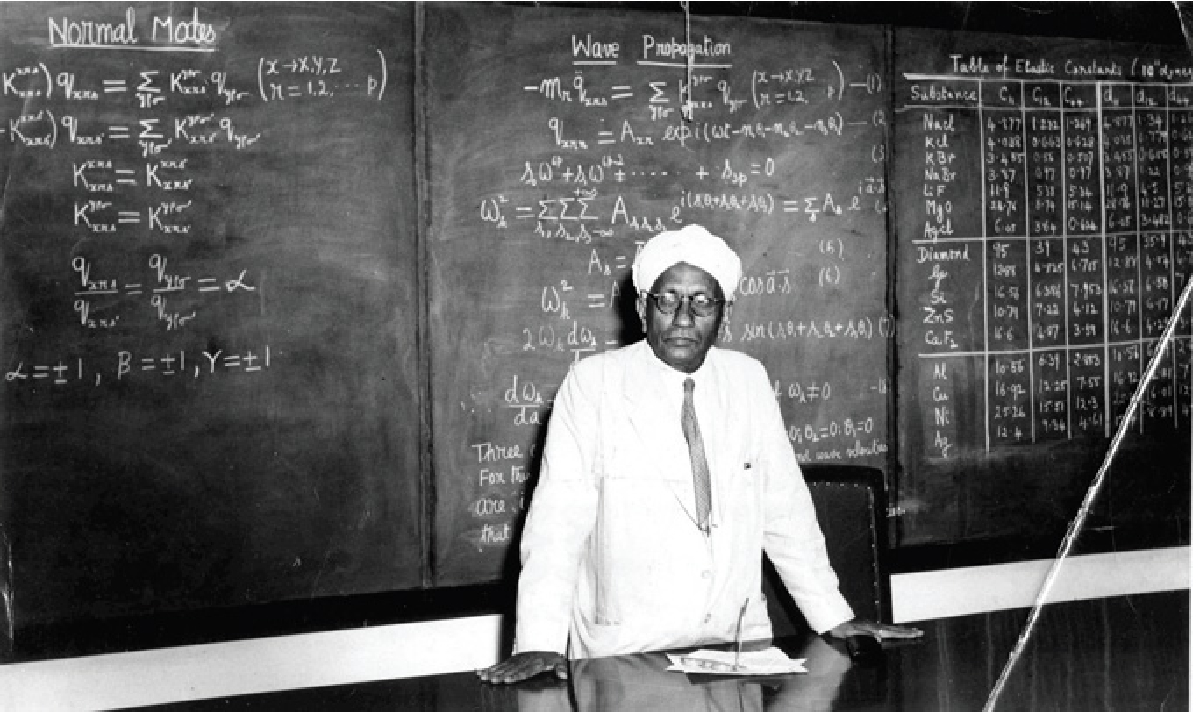
\includegraphics[scale=0.24]{"images/14.jpg"}
\caption{ಉಪನ್ಯಾಸಕರಾಗಿ ರಾಮನ್. ಫೋಟೋ ಕೃಪೆ: ರಾಮನ್‌ ರಿಸರ್ಚ್ ಇನ್ಸ್ಟಿಟ್ಯೂಟ್}\label{chap4-fig01}
\end{figure}

ಹೀಗೆ ರಾಮನ್‍ರವರು ಬೋಧನೆಯನ್ನು ಮನಸಾರೆ ಸ್ವೀಕರಿಸಿದ್ದರು. ಅವರು ವಿದ್ಯಾರ್ಥಿಗಳಲ್ಲಿ ಸ್ಫೂರ್ತಿ ತುಂಬುತ್ತಿದ್ದರು. \enginline{1917}ರಲ್ಲಿ ರಾಮನ್‍ರವರ ಸಹೋದ್ಯೋಗಿಗಳಾಗಿ ಮುಂದೆ \enginline{Ionisation Equation} ಗೆ ಪ್ರಸಿದ್ಧರಾದ ಎಂ. ಎಸ್. ಸಾಹಾ ಮತ್ತು ಎಸ್. ಎನ್. ಬೋಸ್ ರವರು ಇದ್ದರು.


\heading{ರಾಮನ್‍ರವರ ಉಪನ್ಯಾಸಗಳು}

ಸಾರ್ವಜನಿಕ ಉಪನ್ಯಾಸಗಳಲ್ಲಿ ರಾಮನ್‍ರವರದ್ದು ಅದ್ಭುತ ಹಿಡಿತ. ಅವರು ಯಾವುದೇ ವಿಷಯದ ಬಗ್ಗೆಯೂ ಅಂದರೆ, ಉದಾಹರಣೆಗೆ, ‘ಈಜಿಪ್ಟಿನ ಚರಿತ್ರೆ’ ಯ ಬಗ್ಗೆಯೂ ತಟ್ಟನೆ ಉಪನ್ಯಾಸ ನೀಡಬಲ್ಲವರಾಗಿದ್ದರು. ಅವರ ವೈಜ್ಞಾನಿಕ ಉಪನ್ಯಾಸಗಳು ಹಬ್ಬದಂತಿರುತ್ತಿದ್ದವು. ಅವರು ಅದ್ಭುತ ಮನರಂಜನೆ ನೀಡುವ ಕುಶಲಿಯಾಗಿದ್ದರು. ಇಡೀ ಸಭೆಗೆ ಕೇಳಿಸುವಂತೆ ಎತ್ತರದ ಧ್ವನಿಯಲ್ಲಿ ಮಾತನಾಡುತ್ತಿದ್ದರು. ಅವರಿಗೆ ಮೈಕ್ ಬೇಕಾಗಿಯೇ ಇರಲಿಲ್ಲ. ಮೂರ್ತ ಉದಾಹರಣೆಗಳೂ ಅದ್ಭುತ ವಾಗ್ಮಿತೆ, ಹಾಸ್ಯ ಚಟಾಕಿಗಳು ತುಂಬಿರುತ್ತಿದ್ದ ಅವರ ಉಪನ್ಯಾಸಗಳು ಜನಪ್ರಿಯ ಶೈಲಿಯಲ್ಲಿ ಇರುತ್ತಿದ್ದವು. ತುಂಬಿದ ಸಭಿಕರೆಲ್ಲರಿಗೂ ಅವರು ಹೇಳುತ್ತಿದ್ದ ವಿಜ್ಞಾನ ವಿಷಯಗಳು ಅರ್ಥವಾಗಿ\break ಬಿಟ್ಟಿದೆಯೇನೋ ಎನ್ನಿಸುವಂತೆ ಇರುತ್ತಿತ್ತು. ಒಮ್ಮೆ ಅವರು ನನಗೆ ಹೀಗೆಂದರು “ಒಂದು ಒಳ್ಳೆಯ ಸಾರ್ವಜನಿಕ ಭಾಷಣವೆಂದರೆ, ಕೇಳುಗರಿಗೆ ಭಾಷಣಕಾರನು ಹೇಳುವುದೆಲ್ಲ ಅರ್ಥವಾಗಿಬಿಟ್ಟಿದೆ ಎಂಬ ಭ್ರಮೆಹುಟ್ಟಿಸಬೇಕು.” ಅವರು ಮಾಡುತ್ತಿದ್ದದ್ದೂ ಇದೇನೇ. ಸಾವಿರಾರು ಸಭಿಕರಿಗೆ ಇದೇ ಭ್ರಮೆ ಹುಟ್ಟಿಸುವಂತೆ ಅವರ ಭಾಷಣಗಳಿರುತ್ತಿದ್ದವು.

\vskip 2pt

\textbf{ಕಶ್ಯಪ್‍ರವರು, ರಾಮನ್‍ರವರ ಭಾಷಣ ಶೈಲಿಯನ್ನು ಹೀಗೆ ವಿವರಿಸುತ್ತಾರೆ\general{\enginline{-}}}

\vskip 2pt

“ಪೇಟ ಧರಿಸಿದ ಎತ್ತರದ ವ್ಯಕ್ತಿ, ನೇರ, ನೆಟ್ಟನೆ ನಡೆಯಲ್ಲಿ ಸಭೆಯ ವೇದಿಕೆಯತ್ತ ಗಂಭೀರವಾಗಿ ಬಂದರು. ಅವರ ಅಕ್ಕಪಕ್ಕದಲ್ಲಿದ್ದ ಸಂಘಟಕರೊಡನೆ ಬಾಗಿದ ಶರೀರದ ಒಂದೋ, ಎರಡೋ ಮಾತು. ವೇದಿಕೆಯಲ್ಲಿ ಕೂತಕ್ಷಣದಿಂದ ಭಾಷಣ ಮಾಡುವ ತರಾತುರಿ, ವಿಶ್ವಾಸ ತುಂಬಿದ ಮೂರ್ತಿಯಂತಿದ್ದ ವ್ಯಕ್ತಿತ್ವ, ಅವರು ಭಾಷಣ ಶುರು ಮಾಡುವ ಮುನ್ನವೇ ಇವರೊಬ್ಬ ನುರಿತ ಭಾಷಣಕಾರರೆಂದು ಸಭಿಕರಿಗೆ ಮನವರಿಕೆಯಾಗುತ್ತಿತ್ತು.”

ವೇದಿಕೆಯಲ್ಲಿ ಉಪಸ್ಥಿತರಾದೊಡನೆಯೇ ಸಾಂಪ್ರದಾಯಿಕವಾಗಿ ನಡೆಯುವ ಸ್ವಾಗತ,\break ಪರಿಚಯಗಳಿಗೆ ಕಡಿತ. ಇವು ಉದ್ದವಾದಾಗ ಒಂದು ತೀಕ್ಷ್ಣ ನೋಟವು ಸಾಕಾಗಿತ್ತು. ಹೀಗೆ ಸುಂದರ ವಾಗ್ಮಿತೆಯನ್ನು ಹಾಳುಗೈಯುವ ಪರಿಗೆ ಕಡಿವಾಣ ಬೀಳುತ್ತಿತ್ತು. ಭಾಷಣದ ಮೊದಲೆರಡು ವಾಕ್ಯಗಳೇ ವಿದ್ಯುತ್ ಸಂಚಾರವುಂಟು ಮಾಡಿ ಮುಂದಿನ ನುಡಿಗಳಿಗೆ ಆಧಾರವಾಗುತ್ತಿದ್ದವು.

ಅವರು ಅಂದು ಸೋಪಿನ ನೊರೆಗುಳ್ಳೆಗಳ ಬಗ್ಗೆ ಮಾತನಾಡಿದ್ದು ಒಂದು ಕ್ಷಣದಲ್ಲಿ ಒಡೆದು ಹಾಳಾಗುವ ಈ ನೊರೆಗುಳ್ಳೆಯು ಅಂದು ಅರ್ಧ ಗಂಟೆಯ ಕಾಲ ಸಭಿಕರ ಮನಗೆದ್ದಿತು.

ರಾಮನ್ ಕೇಳಿದರು \enginline{—} “ನೀವು ಈ ನೊರೆಗುಳ್ಳೆಯನ್ನು ಬಹಳಕಾಲ ಇರುವಂತೆ ಯೋಚಿಸಿದ್ದೀರಾ” ಈ ಪ್ರಶ್ನೆಯು ಸಭಿಕರಿಗೆ ಹೊಸದು ಅವರು ಬೆರಗಾಗಿ ಕೇಳುತ್ತಿದ್ದರು. ಇದರಲ್ಲಿ ಸಮಸ್ಯೆಯೆಂದರೆ ನೊರೆಗುಳ್ಳೆಯ ಮೇಲಿನ ನೀರಹನಿ ಕೆಳಗೆ ಜಾರಿ ತಳ ಸೇರಬಾರದು” \enginline{-}ರಾಮನ್ ವಿವರಿಸಿದರು. ಬಳಿಕ ತಾವೂ ಮತ್ತು ಫ್ರಾನ್ಸ್ ನ ಕೆಲ ವಿಜ್ಞಾನಿಗಳು ಇಂತಹ ಕ್ಷಣಿಕ ನೊರೆಗುಳ್ಳೆಯನ್ನು ಹಲವಾರು ದಿನಗಳ ಕಾಲ ಕಾಯ್ದಿಟ್ಟುದಾಗಿ ಹೇಳಿದರು. ಈ ನೊರೆಗುಳ್ಳೆಗೆ ಅಭಿಮುಖ ಬಲ ಪ್ರಯೋಗ ಮಾಡಿ ಈ ಸಿದ್ಧಿ ಪಡೆದೆವೆಂದರು.

ಒಂದು ಕ್ಷಣವೂ ಬೇಸರವಾಗಲಿಲ್ಲ. ಭಾಷಣ ಮುಗಿದದ್ದೇ ತಿಳಿಯಲಿಲ್ಲ. ರಾಮನ್‍ರವರ ಭಾಷಣ ಕೇಳುವುದೆಂದರೆ ಭೌತಶಾಸ್ತ್ರಕ್ಕಿಂತ ಮಿಗಿಲಾದದ್ದನ್ನು ಕಲಿತಂತೆ. ಅವರಿಗೆ ಅತ್ಯಂತ ಉತ್ಕೃಷ್ಟ ಪದಪುಂಜಗಳನ್ನು ಬಳಸುವ ತಂತ್ರ ಲಭಿಸಿತ್ತು. ಇದಾವ ಪಠ್ಯ ಪುಸ್ತಕಗಳಲ್ಲೂ ಇರುವುದಿಲ್ಲ. ತಮ್ಮ ಕೋಟನ್ನೂ ಆಗಾಗ ಸರಿಪಡಿಸಿಕೊಳ್ಳುವುದು ಅಭ್ಯಾಸವಾಗಿ ಬಿಟ್ಟಿತ್ತು. ಪ್ರಶ್ನೆಗಳನ್ನು ಆಹ್ವಾನಿಸಿ ಅವಕ್ಕೆ ಅತಿ ಸ್ಪಷ್ಟವಾದ ಉತ್ತರ ನೀಡುತ್ತಿದ್ದರು.”

ಅವರು ಕಟುವಾಗಿ ವಿಮರ್ಶೆ ಮಾಡುತ್ತಿದ್ದರು. \enginline{1958}ರಲ್ಲಿ ಬರೋಡಾದಲ್ಲಿ ನಡೆದ ಇಂಡಿಯನ್ ಅಕಾಡೆಮಿ ಆಫ್ ಸೈನ್ಸಸ್‍ನ ವಾರ್ಷಿಕ ಸಮ್ಮೇಳನದಲ್ಲಿ ಉಚ್ಚಶಕ್ತಿ ಭೌತಶಾಸ್ತ್ರಜ್ಞನೊಬ್ಬನು ಬೋರ್ಡಿನ ತುಂಬ ಗಣಿತ ಸಮೀಕರಣಗಳನ್ನು ತುಂಬಿಸಿದ್ದ. ಇವರು ಎದ್ದು ನಿಂತು “ಅಯ್ಯಾ ನೀನು ಹೇಳಬೇಕೆಂದಿರುವುದನ್ನು ಕೆಲವೇ ವಾಕ್ಯಗಳಲ್ಲಿ ಹೇಳಿ ಮುಗಿಸು. ಹಾಗಾಗದಿದ್ದರೆ ಈ ಉಪನ್ಯಾಸ ಕೇಳಿ ಪ್ರಯೋಜನವಿಲ್ಲ” ಎಂದು ಬಿಟ್ಟರು.

\newpage

ಅರವತ್ತರ ದಶಕದಲ್ಲಿ ಉಸ್ಮಾನೀಯ ವಿಶ್ವವಿದ್ಯಾನಿಲಯ ಹೈದರಾಬಾದಿನಲ್ಲಿ ಅಕಾಡೆಮಿಯ ವಾರ್ಷಿಕ ಸಭೆಯಿತ್ತು. ಅಲ್ಲಿನ ರಾಜ್ಯದ ಗವರ್ನರ್, ವಿಶ್ವವಿದ್ಯಾನಿಲಯದ ಉಪಕುಲಪತಿ ಆಗಿದ್ದರು. ಅವರು ಸ್ವಾಗತ ಭಾಷಣವನ್ನು ಬಹಳ ಉದ್ದ ಮಾಡಿದರು. ಅಲ್ಲದೆ ಅವರ ಭಾಷಣದಲ್ಲಿ ವಿಜ್ಞಾನಿಗಳು ತಮ್ಮ ದಂತಗೋಪುರದಿಂದ ಕೆಳಗೆ ಇಳಿಯಬೇಕೆಂದೂ, ದೇಶದ ಆಮಧು ಪದಾರ್ಥಗಳಿಗೆ ಪರ್ಯಾಯ ಯೋಚಿಸಬೇಕೆಂದೂ, ರಫ್ತು ಮಾಡುವ ವಸ್ತುಗಳಿಗೆ ಉತ್ತೇಜನ ನೀಡುವ ಕೆಲಸ ಮಾಡಬೇಕೆಂದೂ, ರಕ್ಷಣಾ ಸಂಬಂಧಿ ಸಂಶೋಧನೆಗಳನ್ನು ಕೈಗೊಳ್ಳಬೇಕೆಂದೂ ಸಲಹೆ ಮಾಡಿದರು. ಹೀಗೆ ಪುಂಖಾನು ಪುಂಖವಾಗಿ ಸಲಹೆಗಳ ಮಹಾಪೂರವನ್ನೇ ಹರಿಯಿಬಿಟ್ಟರು. ಕೊನೆಯಲ್ಲಿ “ಈಗ ರಾಮನ್‍ರವರು ಭಾಷಣ ಮಾಡುತ್ತಾರೆ. ಅವರ ವಿಷಯ \textit{\general{\enginline{Physiology of Vision}}} ನಿಮಗೆ ಮತ್ತು ನನಗೆ ಅವರು ಹೇಳುವುದು ಅರ್ಥವಾಗದಿರಬಹುದು. ಆದರೆ ಅವರಿಗೆ ನೊಬೆಲ್ ಬಹುಮಾನ ಬಂದಿದೆ. ಅವರೊಬ್ಬ ಹಿರಿಯ ವಿಜ್ಞಾನಿ” ಎಂದರು.

ಈ ಬಗೆಯ ‘ಸ್ವಾಗತ’ವು ರಾಮನ್‍ರವರ ಮನ ಕೆಡಿಸಿತು. ರಾಮನ್‍ರವರ ಭಾಷಣಗಳೆಂದಿಗೂ ಅತಿ ಸರಳ ಭಾಷೆಯಲ್ಲಿ ಎಲ್ಲರಿಗೂ ಅರಿವಾಗುವಂತೆ ಇರುತ್ತಿತ್ತು. ಅವರು ಯಾವುದೇ ಭಾವನೆ ವ್ಯಕ್ತಪಡಿಸದೆ ತಮ್ಮ ವಿಷಯ ಮಂಡನೆಯನ್ನು ಸುಲಲಿತ ಭಾಷೆಯಲ್ಲಿ ಮಾಡಿದರು. ಭಾಷಣದ ಕೊನೆಯಲ್ಲಿ ಗವರ್ನರ್ ಕಡೆ ತಿರುಗಿ ಹೀಗೆಂದರು. “ಮಾನ್ಯ ಗವರ್ನರ್ ಸಾಹೇಬರೇ ನನಗೆ ನೊಬೆಲ್ ಬಹುಮಾನ ಬಂದಾಗ ನನ್ನ ಅಶಿಕ್ಷಿತ ಚಿಕ್ಕಮ್ಮ, ಈ ಬಹುಮಾನ ಬರಲು ನೀನೇನು ಕೆಲಸ ಮಾಡಿದಿ ಎಂದು ಕೇಳಿದರು. ನಾನು ರಾಮನ್ ಎಫೆಕ್ಟ್ ನ ಬಗ್ಗೆ ಅವರಿಗೆ ತಿಳಿಸಿ ಹೇಳಿದೆ. ಅವರು, ಇಂತಹ ಸರಳ ವಿಷಯವನ್ನು ಕಂಡು ಹಿಡಿದಿದ್ದಕ್ಕಾಗಿ ಇಷ್ಟು ದೊಡ್ಡ ಬಹುಮಾನ ಕೊಟ್ಟರೇ ಎಂದು ಆಶ್ಚರ್ಯ ವ್ಯಕ್ತಪಡಿಸಿದರು. ಗವರ್ನರ್ ಸಾಹೇಬರೇ ನಿಮಗೆ ನಾನು ಇಂದು ಮಾಡಿದ ಭಾಷಣ ಅರ್ಥವಾಗಿದೆಯೆಂದು ಊಹಿಸುತ್ತೇನೆ.” ಸಭೆಯು ಕಿವಿಗಡಚಿಕ್ಕುವಂತೆ ಚಪ್ಪಾಳೆ ತಟ್ಟಿತು.

ಅನೇಕ ವರ್ಣರಂಜಿತ ಸ್ಲೈಡುಗಳು, ಚಿತ್ರಗಳೂ ಒಳಗೊಂಡಂತೆ ರಾಮನ್‍ರವರ ಉಪನ್ಯಾಸಗಳ ತಯಾರಿಯು ಅತಿ ಶ್ರಮದಾಯಕವಾಗಿರುತ್ತಿತ್ತು. ಅವರಿಗೆ ಬೇಕಾದ ವರ್ಣ ಚಿತ್ರಗಳನ್ನು ನಾನೇ ತಯಾರಿಸಿ ಕೊಡುತ್ತಿದ್ದೆ. ನಾನೊಮ್ಮೆ ರತ್ನಗಳು ಸೂಸುವ ವರ್ಣಗಳನ್ನು ಫೋಟೋ ತೆಗೆದಿದ್ದೆ. ರಾಮನ್‍ರವರು ಅದನ್ನು ಸ್ಲೈಡು ಮಾಡಲು ಬಾಂಬೆಗೆ ತೆಗೆದೊಯ್ದರು. ಸ್ಲೈಡುಗಳು ಬಹಳ ಚೆನ್ನಾಗಿ ಮೂಡಿ ಬಂದವು. ರಾಮನ್‍ರವರಿಗೆ ಭಾರಿ ಖುಷಿಯಾಯಿತು. ಅವರು ತಕ್ಷಣವೇ ಬೆಂಗಳೂರಿಗೆ ಎಕ್ಸ್ ಪ್ರೆಸ್ ಟೆಲಿಗ್ರಾಂ ಕಳುಹಿಸಿ ತಮ್ಮ ಸಂತೋಷ ವ್ಯಕ್ತಪಡಿಸಿದರು. ಅವರ ಮೆಚ್ಚುಗೆಗಳಲ್ಲಿ ಕಪಟವಿರುತ್ತಿರಲಿಲ್ಲ. ಒಳ್ಳೆಯ ಕೆಲಸಕ್ಕೆ ತಕ್ಷಣ ಮೆಚ್ಚುಗೆ ಸಿಗುತ್ತಿತ್ತು. ಅಲ್ಲದೆ ಸಾರ್ವಜನಿಕವಾಗಿ ಇಂತಹವರು ಒಳ್ಳೆಯ ಕೆಲಸಮಾಡಿದ್ದಾರೆ, ಅವರು ಅದ್ಭುತ ಆವಿಷ್ಕಾರ ಮಾಡಿದ್ದಾರೆ ಎಂದು ಮುಕ್ತವಾಗಿ ಹೊಗಳುತ್ತಿದ್ದರು.

ರಾಮನ್ ಸಂಸ್ಥೆಯಲ್ಲಿ ಉಪನ್ಯಾಸ ಕೊಠಡಿ ಬಹಳ ಚೆನ್ನಾಗಿತ್ತು. ಒಳ್ಳೆಯ ಗಾಳಿ ಬೆಳಕು ಇರುತ್ತಿತ್ತು. ಕೊಠಡಿಯ ಒಂದು ಬದಿಯಲ್ಲಿ ಗಾಜಿನ ಬೋರ್ಡ್ ಒಂದು ಕೊನೆಯಿಂದ ಇನ್ನೊಂದು ಕೊನೆಯವರೆಗೆ ಹರಡಿತ್ತು. ತೇಗದ ಮರದ ಉದ್ದನೆಯ ಮೇಜು ಭಾಷಣಕಾರರ ಮುಂದೆ ಇರುತ್ತಿತ್ತು. ಸ್ಯಾಟಿನ್ ಬಟ್ಟೆ ಹಾಕಿದ ಒಂದು ನೂರು ತೇಗದ ಕುರ್ಚಿಗಳು ಮೆಟ್ಟಿಲು ಮೆಟ್ಟಿಲುಗಳಾಗಿ ಮೇಲೇರುವ ಸಭಾಮಂದಿರದಲ್ಲಿ ಜೋಡಿಸಿದ್ದವು. ಈ ಕುರ್ಚಿಗಳಲ್ಲಿ ಅಗಲವಾಗಿ ಎರಡೂ ಕೈಗಳನ್ನು ಇಟ್ಟುಕೊಳ್ಳುವಂತೆ ಕೈಒತ್ತುಗಳಿದ್ದವು. ಇವೆಲ್ಲ ರಾಮನ್‍ರವರ ಇಷ್ಟದಂತೆ ಸಭಿಕರ ಅನುಕೂಲಕ್ಕಾಗಿ ಮಾಡಿದವು. ಇಲ್ಲೇ ರಾಮನ್‍ರವರು ತಮ್ಮ ಸಾಮಾನ್ಯ ಉಪನ್ಯಾಸಗಳನ್ನೂ ಮತ್ತು ವಿಶೇಷ ಉಪನ್ಯಾಸಗಳನ್ನೂ ನೀಡುತ್ತಿದ್ದರು.

ಪ್ರತಿವರ್ಷ ಅಕ್ಟೋಬರ್ ತಿಂಗಳಿನಲ್ಲಿ ಗಾಂಧಿ ಸ್ಮಾರಕ ಉಪನ್ಯಾಸವನ್ನು ನೀಡುತ್ತಿದ್ದರು. ಗಾಂಧಿ ಪೀಸ್ ಫೌಂಡೇಶನ್ ರವರು ಇದಕ್ಕಾಗಿ ದತ್ತಿಯನ್ನು ಇಟ್ಟಿದ್ದರು. ಈ ಉಪನ್ಯಾಸಗಳಿಗೆ ಸಭೆಯ ತುಂಬ ಜನರು ಇರುತ್ತಿದ್ದರು. ಇದೊಂದೇ ಸಂದರ್ಭದಲ್ಲಿ ಸಾರ್ವಜನಿಕರು ರಾಮನ್‍ರವರ ಭಾಷಣ ಕೇಳಬಹುದಾಗಿತ್ತು. ಈ ಉಪನ್ಯಾಸಗಳಿಗೆ ಮುಕ್ತ ಸ್ವಾಗತವಿತ್ತು. ಆದರೆ ಮೊದಲು ಬಂದವರಿಗೆ ಮೊದಲ ಆದ್ಯತೆಯ ಪ್ರಕಾರ ಟಿಕೆಟ್ ವ್ಯವಸ್ಥೆಯಿತ್ತು. ರಾಮನ್‍ರವರ ಕಾರ್ಯಕ್ಷೇತ್ರದ ವಿಷಯವೋ ಅಥವಾ ಇನ್ನಾವುದೇ ರೋಚಕ ವಿಷಯವನ್ನೋ ಅವರು ಉಪನ್ಯಾಸಕ್ಕಾಗಿ ಆಯುತ್ತಿದ್ದರು. ಈ ವಿಷಯವನ್ನೇ ಅದ್ಭುತವಾಗಿ ಮಂಡಿಸುತ್ತಿದ್ದರು. ಒಮ್ಮೆ \textit{\general{\enginline{Physiology of Vision}}} ಬಗ್ಗೆಯೂ, ಭೂಕಂಪಗಳು, ವಾತಾವರಣ, ಧ್ವನಿ, ಮಾತು ಮತ್ತು ಭಾಷೆಗಳ ಬಗ್ಗೆಯೂ ವಿಷಯಗಳ ಆಯ್ಕೆ ಇರುತ್ತಿತ್ತು. ಅವರ ಕೊನೆಯ ಗಾಂಧಿ ಉಪನ್ಯಾಸವು ಅಕ್ಟೋಬರ್ \enginline{2, 1970}ರಲ್ಲಿ ಇತ್ತು.


\heading{ರಾಮನ್‍ರವರ ವ್ಯಕ್ತಿತ್ವದ ಕುರಿತು ಕೆಲವು ಅನಿಸಿಕೆಗಳು}

\vskip 2pt

ರಾಮನ್‍ರವರನ್ನು ಹತ್ತಿರದಿಂದ ಬಲ್ಲವರಿಗೂ, ದೂರದಿಂದ ಕಂಡವರಿಗೂ, ಅವರ ಕೆಲವು ವಿಶೇಷ ಗುಣಗಳು ಎದ್ದು ಕಾಣುವಂತಿದ್ದವು. ಅವರಿಗೆ ಮಗುವಿನಂತಹ ಕುತೂಹಲವಿತ್ತು. ಪ್ರಕೃತಿಯನ್ನು ಅರ್ಥಮಾಡಿಕೊಳ್ಳಲೂ, ನಿಗೂಢ ವಿಷಯಗಳಲ್ಲೂ ಅವರಿಗೆ ಜೀವನದುದ್ದಕ್ಕೂ ತೀವ್ರ ಆಸಕ್ತಿಯಿದ್ದಿತು. ಈ ಬಗೆಯ ಪ್ರೇರಣೆಯಿರುವವರಿಗೆ ಪ್ರಕೃತಿಯೇ ರೋಚಕವಾಗಿ ಕಾಣುತ್ತದೆ. ಖನಿಜಗಳಲ್ಲಿ ವರ್ಣಗಳು ಉಂಟಾಗುವುದು ಹೇಗೆ, ಹಕ್ಕಿಗಳಲ್ಲೂ, ಚಿಟ್ಟೆಗಳಲ್ಲೂ ಬಣ್ಣಗಳಿರುವುದು ಹೇಗೆ, ಸಾಗರದ ನೀಲಿ ಬಂದದ್ದು ಹೇಗೆ\enginline{-} ಈ ಬಗೆಯ ಮೂಲ ಪ್ರಶ್ನೆಗಳೇ ರಾಮನ್‍ರವರ ಮುಖ್ಯ ಸಂಶೋಧನಾ ವಿಷಯಗಳು ಅವರಿಗೆ ಪ್ರಕೃತಿಯ ಈ ಭೌತಿಕ ಸಂಪತ್ತನ್ನು ವ್ಯೊಮ ವಿಜ್ಞಾನಕ್ಕೆ ವ್ಯಯಿಸುವುದು ಸ್ವಲ್ಪವೂ ಇಷ್ಟವಿರಲಿಲ್ಲ. ಪ್ರಕೃತಿಯ ವಿಶ್ಲೇಷಣೆ ಇಲ್ಲಿನ ಜೀವಿಗಳಿಗೆ ಒಳ್ಳೆಯದುಂಟು ಮಾಡುತ್ತದೆ. ಇದನ್ನು ಬಿಟ್ಟವು ಜೀವಸಂಕುಲಕ್ಕೆ ಹಿತವಲ್ಲ ಎಂಬ ಭಾವನೆ ಅವರಿಗಿತ್ತು.

ಅವರಿಗಿದ್ದ ವಿಶೇಷ ಗುಣಗಳಾದ ನವಿರಾದ ಹಾಸ್ಯ ಪ್ರಜ್ಞೆ, ತೀಕ್ಷ್ಣ ವ್ಯಂಗ್ಯ, ಪ್ರಕೃತಿ ಪ್ರೇಮಗಳು, ಯಾವುದೇ ವಿಷಯದ ಬಗ್ಗೆ ಮಾತನಾಡತೊಡಗಿದಾಗ ಹಾಸುಹೊಕ್ಕಾಗಿರುತ್ತಿದ್ದವು. ಒಮ್ಮೆ ಅವರು ಗ್ರಾಮ ಪ್ರದೇಶಗಳು ಮತ್ತು ವಾತಾವರಣದ ಬಗ್ಗೆ ಮಾತನಾಡಬೇಕಾದಾಗ ಹೀಗೆಂದರು\enginline{-}

“ನಗರಗಳಲ್ಲಿ ವಾಸಿಸುವವರಿಗೆ ಹವಾಮಾನವು ಒಂದು ಅನಾನುಕೂಲವಷ್ಟೆ. ಇದಕ್ಕಾಗಿ ಸ್ವಲ್ಪ ಯೋಚಿಸಿ ಊರುಗೋಲಿನ ಬದಲು ಕೊಡೆಯೊಂದನ್ನು ಮನೆಯಿಂದ ಹೊರಗೆ ತೆಗೆದುಕೊಂಡು ಹೋದರಾಯಿತು. ಇದನ್ನು ಬಿಟ್ಟು ಹವಾಮಾನದ ಬಗ್ಗೆ ನಗರ ವಾಸಿಗೆ ಇದರ ಅರಿವೇ ಬರುವುದಿಲ್ಲ. ಆಕಾಶದಲ್ಲಿನ ವಿವಿಧ ವಿನ್ಯಾಸಗಳು ಅತಿ ಸುಂದರ. ಸೂರ್ಯೋದಯ, ಸೂರ್ಯಾಸ್ತಗಳು ನಗರ ವಾಸಿಗಳಿಗೆ ಒಂದಾದ ಮೇಲೊಂದು ಘಟನೆಗಳು ಮಾತ್ರ. ಆಕಾಶವಾದರೋ ಅಲ್ಲಲ್ಲಿ ಟೆಲಿಫೋನ್, ವಿದ್ಯುತ್ ತಂತಿಗಳ ನಡುವೆ ಕಾಣುವುದಷ್ಟೆ. ಅವನಿಗೆ ಕಾಣುವ ತಾರೆಗಳು, ಬೆಳ್ಳಿ ತೆರೆಯ ಮೇಲೆ ಮಾತ್ರ. ಸೂರ್ಯ, ಚಂದ್ರರು ಇದ್ದಾರೆಂದು ಗೊತ್ತಿದ್ದರೂ ಅವು ಯಾವಾಗ ಎಲ್ಲಿರುತ್ತವೆಂದು ತಿಳಿಯುವ ಗೋಜಿಗೆ ಹೋಗುವುದಿಲ್ಲ.”

ವಿಜ್ಞಾನದ ಬೆಳವಣಿಗೆ ಮತ್ತು ಅದರ ಮೂಲಭೂತ ಪ್ರಶ್ನೆಗಳಿಗೆ ರಾಮನ್‍ರವರ ಅನಿಸಿಕೆಗಳು ಅವರ ಸಾರ್ವಜನಿಕ ಭಾಷಣಗಳಲ್ಲೂ ಮತ್ತು ಖಾಸಗಿ ಮಾತುಕತೆಗಳಲ್ಲೂ ವ್ಯಕ್ತವಾಗುತ್ತಿದ್ದವು. ವಿಜ್ಞಾನದ ಆವಿಷ್ಕಾರಗಳ ಬಗ್ಗೆ ರಾಮನ್‍ರವರ ಹೇಳಿಕೆ ಈ ರೀತಿ ಇತ್ತು.

“\enginline{-}ಹೊರಗಡೆಯ ಜಗತ್ತು ವಿಜ್ಞಾನಿಯ ಅತಿ ಪ್ರಮುಖ ಆವಿಷ್ಕಾರಗಳಿಗೆ ನೀಡುವ ಸ್ವಾಗತವು ಹಲವಾರು ಬಾರಿ ಗೌರವಪೂರ್ಣ ಶ್ಲಾಘನೆಯಂತಿರುವುದಿಲ್ಲ. ಆಲೋಚನಾ ಶೂನ್ಯರೂ, ಅಸೂಯೆ ಪಡುವವರೂ ಮಾಡುವ ಕೆಲಸವೆಂದರೆ, ಆವಿಷ್ಕಾರವನ್ನು ಅದೊಂದು ಆಕಸ್ಮಿಕವೆಂದು ಬಿಂಬಿಸುವುದು ಅಥವಾ ಅದೃಷ್ಟದ ಕ್ಷಣವೆಂದೂ (ಲಾಟರಿ ಹೊಡೆದ ಹಾಗೆ) ಎಂದೆನ್ನುವುದು. ಇಂತಹ ಹೇಳಿಕೆಗಳು ಅರ್ಥವಿಲ್ಲದ್ದು ಅಥವಾ ಖಂಡಿಸ ಬೇಕಾದಂತಹವು. ಒಂದು ವೈಜ್ಞಾನಿಕ ಆವಿಷ್ಕಾರವು, ಆಕಸ್ಮಿಕವಾಗಿ ಘಟಿಸುವಂತಹದು ಎಂಬ ಆಲೋಚನೆಯೇ ತಪ್ಪು. ಏಕೆಂದರೆ ಈ ‘ಆಕಸ್ಮಿಕವು’ ಅದರ ಹಿಂದೆ ಶ್ರಮಗೈದ ವಿಜ್ಞಾನಿಗೇ ಏಕೆ ಉಂಟಾಗುತ್ತದೆ, ಎಂಬುದಕ್ಕೆ ಉತ್ತರವಿಲ್ಲ. ವಿಜ್ಞಾನ ಸಂಶೋಧಕನಿಗೆ ಜ್ಞಾನದ ಮತ್ತು ಸತ್ಯದ ಅನ್ವೇಷಣೆಯೇ ಗುರಿ. ಅವನು ಆಯ್ದುಕೊಂಡ ಕ್ಷೇತ್ರದಲ್ಲಿ ಅವನ ಶ್ರಮ ವ್ಯಯಿಸಿ ಸ್ವಲ್ಪವಾದರೂ ಹೊಸತನ್ನು ಸಾಧಿಸಬೇಕೆಂಬ ಹಂಬಲ ಅವನದು. ಆವಿಷ್ಕಾರಗಳನ್ನು ಆಕಸ್ಮಿಕಗಳೆಂದು ವಿಮರ್ಶಿಸುವವರು, ನೈಜ ಸತ್ಯ ಶೋಧನೆಯನ್ನು ಗಮನದಲ್ಲಿ ನಿರಂತರವಾಗಿ ಹಿಡಿದಿಡುವುದೇ ವೈಜ್ಞಾನಿಕ ಸಂಶೋಧನೆಯಾಗುತ್ತದೆಂಬುದನ್ನು ಮರೆಮಾಚುತ್ತಾರೆ. ಈ ಬಗೆಯ ನಿರಂತರ ಗಮನ ಸಾಧ್ಯಕ್ಕೆ, ಸಾಧಕನೊಬ್ಬನಿಗೆ ವಿಷಯದ ವಿಸ್ತೃತ ಜ್ಞಾನವೂ ಇರಬೇಕಾಗುತ್ತದೆ. ಬಹಳ ಎಚ್ಚರಿಕೆಯಿಂದ ಕಾರ್ಯವಿಧಾನ ಹಾಕಿಕೊಂಡ ಹೊರತು ವೈಜ್ಞಾನಿಕ ಆವಿಷ್ಕಾರಗಳು ಕೈಗೆಟುಕುವುದು ಕಷ್ಟ. ಅನೇಕ ತಿಂಗಳುಗಳ ಅಥವಾ ವರ್ಷಗಳ ನಿಯಮಿತ ಅಧ್ಯಯನ ಮತ್ತು ಆ ವಿಶೇಷ ವಿಷಯದಲ್ಲಿ ಸಂಶೋಧನೆಗಳ ಫಲವಾಗಿಯೇ ಇವು ಕೈಗೆಟುಕಲು ಸಾಧ್ಯ.”

“ವಿಜ್ಞಾನವು ಅತಿ ವಿಶಿಷ್ಠ ಮತ್ತು ಕ್ಲಿಷ್ಟ ಮನೆಯೊಡತಿಯಿದ್ದಂತೆ” ಎಂಬುದು ರಾಮನ್ನರ ಬಹುವಾಚಿಕವಾಗಿತ್ತು. “ಅವಳ ಸಂಪತ್ತಿಗಾಗಿ ಪ್ರೀತಿಸಿದರೆ ಒಲಿಯುವವಳಲ್ಲ. ಅವಳು ಹೇಗಿದ್ದಾಳೋ ಹಾಗೆಯೇ ಪ್ರೀತಿ ತೋರಿದರೆ ಮಾತ್ರ ಒಲಿದಾಳು. ಅಲ್ಲದೆ ಎಂದಿಗೂ ಪೂರ್ಣವಾಗಿ ತನ್ನ ಗುಟ್ಟು ಬಿಟ್ಟುಕೊಡುವವಳಲ್ಲ. ಕೊಂಚ, ಕೊಂಚವಾಗಿ ಮಾತ್ರ ಗುಟ್ಟು ಹೊರಬಿದ್ದೀತು.” ವಿವೇಚನೆಯುಳ್ಳ ಹಲವಾರು ವಿಮರ್ಶಕರು ದಾಖಲಿಸಿರುವಂತೆ ರಾಮನ್‍ರವರ ಬಗ್ಗೆ ಮಾತನಾಡುವಾಗ ಮತ್ತು ಅವರನ್ನು ಮೌಲ್ಯಮಾಪನ ಮಾಡುವಾಗ, ಹೀಗೆ ಹೇಳುವವರಿದ್ದಾರೆ.\enginline{-} “ಜ್ಞಾನ ಶಿಸ್ತಿಗೆ ಹಲವಾರು ಶತಮಾನಗಳ ಬಳಿಕ ನಮ್ಮ ಭಾರತ ದೇಶವು ನೀಡಿದ ಕೊಡುಗೆ ರಾಮನ್‍ರವರು.” ನಾವು ಅವರನ್ನು ಒಬ್ಬ ಅದೃಷ್ಟವಂತ, ಗೆಲುವು ಸಾಧ್ಯಮಾಡಿಕೊಂಡ ವಿಜ್ಞಾನಿಯಂತೆ ನೋಡುವ ತಪ್ಪು ಮಾಡಬಾರದು. ಅನೇಕ ಮಂದಿ ಸಫಲ ವಿಜ್ಞಾನಿಗಳಿದ್ದಾರೆ, ಸಫಲ ವ್ಯಾಪಾರಿಗಳಿದ್ದಾರೆ, ಹಾಗೆಯೇ ಸಫಲ ರಾಜಕಾರಣಿಗಳೂ ಇದ್ದಾರೆ. ಆದರೆ ರಾಮನ್ ಹೀಗಲ್ಲ. ಇಂತಹವರು ಆಗಾಗ ಜನ್ಮ ಪಡೆಯುವುದಿಲ್ಲ. ವೃತ್ತಿ ಸಫಲತೆಯತ್ತ ಗಮನ ಹರಿಸುವ ಜಗತ್ತು ರಾಮನ್‌ನಂತಹ ದೈತ್ಯ ಪ್ರತಿಭೆಯ ಅಂಕುಡೊಂಕುಗಳನ್ನೂ ತೀಕ್ಷ್ಣ ಪ್ರತಿಭೆಯನ್ನೂ ಗುರುತಿಸಲಾಗದಿದ್ದಲ್ಲಿ ಈ ವಿದ್ಯಮಾನವನ್ನು ಹೀಗೆ ಉದಾಹರಿಸಬಹುದೇನೋ.

“ಗೌರಿಶಂಕರ ಶಿಖರದ ಮೇಲೆ ನೀವು ಗೋಲ್ಫ್ ಆಡಲಾಗದಿದ್ದರೆ ಅದು ಗಿರಿಶಿಖರದ ತಪ್ಪಲ್ಲ.”

ರಾಮನ್‍ರವರು ತೀವ್ರ ಆಶಾಭಂಗಗಳ ನಡುವೆ, ಹತಾಶೆಗಳ ನಡುವೆ, ಅನೇಕ ಸಂಕಷ್ಟಗಳನ್ನು ದಾಟಿ, ವೃತ್ತಿ ಜೀವನದಲ್ಲಿ ಉತ್ತುಂಗಕ್ಕೆ ಏರಿದವರೆಂಬುದನ್ನು ಅನೇಕರು ಅರಿಯರು. ಒಮ್ಮೊಮ್ಮೆ ಅವರು ತಮ್ಮ ಹಿಂದಿನ ಜೀವನವನ್ನು ಮೆಲಕು ಹಾಕುತ್ತಿದ್ದರು. ಹಿಂತಿರುಗಿ ನೋಡಿದಾಗಲೆಲ್ಲಾ, ತಾವು ಅನುಭವಿಸಿದ ನಿರಾಶೆ, ಆಶಾಭಂಗಗಳು, ಹೋರಾಟ ಮತ್ತು ಪರಿಹರಿಸಿಕೊಂಡ ಸಂಕಷ್ಟಗಳೇ ನೆನಪಿಗೆ ಬರುತ್ತವೆಂದು ಅವರು ಹೇಳುತ್ತಿದ್ದರು. ನಂಬಲಾಗದಿದ್ದರೂ ನಿಜಾಂಶವೊಂದಿದೆ. ಎಲ್ಲೋ ಸ್ವಲ್ಪ ಆತ್ಮವಿಶ್ವಾಸ ಮತ್ತು ಸಫಲತೆಗಳು ಹಿನ್ನೆಲೆಗಿದ್ದರೂ ಅವರು ಹೀಗೆನ್ನುತ್ತಿದ್ದರು\enginline{-} “ಖಂಡಿತವಾಗಿಯೂ ಗೆಲುವಿನ ಕ್ಷಣಗಳಿವೆ. ನನ್ನ ದಾರಿದ್ರ್ಯ ಮತ್ತು ಬಡ ಪ್ರಯೋಗಾಲಯಗಳೆ ನಾನು ಏನಾದರೂ ಸಾಧಿಸಬೇಕೆಂಬ ಛಲ ಕೊಟ್ಟಿತು.” ಅವರ ಜೀವನ ಚರಿತ್ರೆಯ ಟಿಪ್ಪಣಿಯನ್ನು ಅವರ ಸಹೋದ್ಯೋಗಿ\-ಗಳು ತಯಾರಿಸಿದ್ದರು. ಅದನ್ನೋದಿದ ಅವರು “ಈ ಟಿಪ್ಪಣಿಯಲ್ಲಿ ನಾನು ಒಂದು ಗೆಲುವಿನಿಂದ ಮತ್ತೊಂದು ಗೆಲುವಿಗೆ ಚಿನ್ನದ ಕುರ್ಚಿಯಲ್ಲಿ ಕುಳಿತು ಎಲ್ಲೂ ಕಣ್ಣೀರಿನ ಕುರುಹೇ ಇಲ್ಲದೆ, ಸಾಗುತ್ತಿದ್ದೆ\-ನೆಂದು ಚಿತ್ರಿತವಾಗಿದೆ. ಜೀವನ ಹೀಗಿದ್ದಿದ್ದರೆ ಎಷ್ಟು ಚೆನ್ನಾಗಿರುತ್ತಿತ್ತು! ಆದರೆ ನನ್ನ ಜೀವನ ಹೀಗಿರಲಿಲ್ಲವೆಂದು ನನಗೆ ಗೊತ್ತು.”

ವಿಜ್ಞಾನಿಗಳ ಜೀವತಾವಧಿಯಲ್ಲಿ, ವೈಜ್ಞಾನಿಕ ರಂಗದ ಗೆಲುವುಗಳೂ ಸಂಕಷ್ಟಗಳ ಜೊತೆಯಲ್ಲಿ ಸೇರಿಕೊಂಡೇ ಬರುತ್ತವೆ. ರಾಮನ್‍ರವರ ಜೀವನವು ಇದಕ್ಕೆ ಹೊರತೇನಲ್ಲ. ಅವರು ಟಾಟಾ ವಿಜ್ಞಾನ ಸಂಸ್ಥೆಯಲ್ಲೂ, ಕಲ್ಕತ್ತದಲ್ಲೂ ಕೆಟ್ಟ ದಿನಗಳನ್ನು ಎದುರಿಸ ಬೇಕಾಯಿತು. ಇದರಿಂದ ಅವರಿಗೆ ಭಾವನಾತ್ಮಕ ಆಘಾತವುಂಟಾಯಿತು. ಇವು ವಿಜ್ಞಾನ ರಂಗದಿಂದ ಬಂದವಲ್ಲ, ಆಗಿನ ಕಾಲದ ವಿಜ್ಞಾನ ರಂಗದ ರಾಜಕೀಯದಿಂದ ಉಂಟಾದವು.

\enginline{1928}ರಲ್ಲಿ ರಾಮನ್ ಪರಿಣಾಮವು ಆವಿಷ್ಕಾರಗೊಂಡು ನೊಬೆಲ್ ಬಹುಮಾನ ಬಂದನಂತರ, ರಾಮನ್‍ರವರ ಕೀರ್ತಿ ಉತ್ತುಂಗಕ್ಕೆ ಏರಿತು. ದೇಶ ವಿದೇಶಗಳಲ್ಲಿ ಅವರು ಪ್ರಸಿದ್ಧರಾದರು. ರಾಮನ್‍ರವರು ಏರಿದ ಎತ್ತರ ಮತ್ತು ಅವರಿಗೆ ಸಿಕ್ಕ ಮಾನ್ಯತೆಯು ಕೆಲವರಿಗೆ ಅಸೂಯೆ ಹುಟ್ಟಿಸಿದ್ದು ಸಹಜ. ಇದರಿಂದ ರಾಮನ್‍ರವರಿಗೆ ತುಂಬಾ ತೊಂದರೆಯ ದಿನಗಳು ಎದುರಾದವು. ಬಂಗಾಳದ ವಿದ್ಯಾರ್ಥಿಗಳಿಗೆ ರಾಮನ್ ಅನ್ಯಾಯ ಮಾಡುತ್ತಿದ್ದಾರೆಂದು ಕೆಲವರು ಭಾವಿಸಿದರು. ಆಯ್ಕೆ ಮಾಡುತ್ತಿದ್ದ ವಿದ್ಯಾರ್ಥಿಗಳ ಬಗ್ಗೆ ಅವರು ಪಕ್ಷಪಾತ ತೋರಿಸುತ್ತಾರೆಂಬ ಆರೋಪವೂ ಇತ್ತು. ರಾಮನ್‍ರವರ ಘನತೆ ಗೌರವಗಳು ಹೆಚ್ಚಾದಂತೆಲ್ಲಾ, ಇಂತಹ ಆರೋಪಗಳೂ ಹೆಚ್ಚಾದವು. ವಿವೇಚನೆ\-ಯುಳ್ಳ ಮಹನೀಯರಾರೂ ಇದರಿಂದ ವಿಚಲಿತರಾಗುವುದಿಲ್ಲ. ಆದರೂ ಒಮ್ಮೊಮ್ಮೆ ಇಂತಹ ಆರೋಪಗಳೇ ಕಹಿ ಸಂದರ್ಭಗಳನ್ನು ಸೃಜಿಸಿದ್ದುಂಟು. ಇಂಡಿಯನ್ ಅಸೋಸಿಯೇಷನ್ ಆಫ್ ಕಲ್ಟಿವೇಶನ್ ಆಫ್ ಸೈನ್ಸ್ ರಾಮನ್‍ರವರ ಅತ್ಯುತ್ತಮ ವೈಜ್ಞಾನಿಕ ಕಾರ್ಯಕ್ಕೆ ತಳಹದಿ ಒದಗಿಸಿತ್ತು. ಈ ಸಂಸ್ಥೆಯಿಂದ ಅವರು ಸದ್ದಿಲ್ಲದೆ ಹೊರಬೀಳಬೇಕಾಯಿತು. ಇದೂ ಅಲ್ಲದೆ ಸಾರ್ವಜನಿಕವಾಗಿ ಕಟು ಮಾತುಗಳಿಗೆ ಉತ್ತರ ನೀಡಬೇಕಾಯಿತು. ಒಂದು ಘಟ್ಟದಲ್ಲಿ ಅವರು “ನಾನು, ಇಡೀ ದೇಶಕ್ಕೆ ಭೌತಶಾಸ್ತ್ರ ಅಧ್ಯಯನ ಪೀಠ ಮಾಡದೆ ಬರೀ ಬಂಗಾಳ ಭೌತಶಾಸ್ತ್ರ ಅಧ್ಯಯನ ಪೀಠ ಮಾಡಬಹುದಾಗಿತ್ತು. ಆಗ ನೊಬೆಲ್ ಬಹುಮಾನವು ಪೂರ್ವದೇಶಕ್ಕೆ ಸೂಯಜ್ ಕಾಲುವೆಯಿಂದ ಈಚೆಗೆ ಖಂಡಿತ ಬರುತ್ತಿರಲಿಲ್ಲವೆಂದು ಖಂಡಿತವಾಗಿ ಹೇಳಬಲ್ಲೆ.”

ಕಲ್ಕತ್ತದ ಪ್ರಸಿದ್ಧ ಪತ್ರಿಕೆಯೊಂದು ತನ್ನ ಸಂಪಾದಕೀಯದಲ್ಲಿ ರಾಮನ್‍ರವರ ಬಗ್ಗೆ ಕಟು ವಿಮರ್ಶೆ ಮಾಡಿತು\enginline{-} “ವಿಜ್ಞಾನಿಯೊಬ್ಬ ಒಳ್ಳೆಯ ಆಡಳಿತಗಾರನಾಗ ಬೇಕಿಲ್ಲ. ವಿಜ್ಞಾನಿಯೊಬ್ಬನ ಸಾಧನೆಗಳು, ಅವನಿಗೆ ದಿನನಿತ್ಯದ ಆಡಳಿತಾತ್ಮಕ ಕುಶಲತೆಗಳನ್ನು ನೀಡುವುದಿಲ್ಲ. ಆದರೆ ಇವು ಖಾಸಗಿ ಜೀವನದಲ್ಲೂ, ಸಾರ್ವಜನಿಕ ಜೀವನದಲ್ಲೂ ಅಗತ್ಯವಾಗಿರುತ್ತವೆ.” ಆದರೂ ಕಲ್ಕತ್ತದಲ್ಲಿ ಅನೇಕ ಪ್ರಸಿದ್ಧರೂ, ವಿಶಾಲ ಹೃದಯಿಗಳೂ ಇದ್ದರು. ಅವರಿಗೆ ಸಾಕಷ್ಟು ವಿಶಾಲದೃಷ್ಠಿಯೂ ಇದ್ದಿತು. ರಾಮನ್‍ರವರು ವಿಶೇಷ ಪ್ರತಿಭಾಶಾಲಿಗಳೆಂದೂ, ಅವರ ಕಾರ್ಯಶೈಲಿಯನ್ನು ಗೌರವದಿಂದ ಕಾಣಬೇಕೆಂದೂ, ಅವರ ರೀತಿ ನೀತಿಗಳು ಇತರೆ ಸಾಮಾನ್ಯ ಜನರಂತೆ ಇರಬೇಕಾದ ಅಗತ್ಯವಿಲ್ಲವೆಂದೂ ಅವರುಗಳು ಅಭಿಪ್ರಾಯ ವ್ಯಕ್ತಪಡಿಸಿದ್ದರು.

\enginline{1933}ರಲ್ಲಿ ಟಾಟಾ ವಿಜ್ಞಾನ ಸಂಸ್ಥೆಯಲ್ಲಿ ನಿರ್ದೇಶಕ ಆಗಿ ನೇಮಕಗೊಂಡಾಗಲೂ ಅವರು ಸಂಕಷ್ಟದ ದಿನಗಳನ್ನು ಎದುರಿಸಬೇಕಾಯಿತು. ಇಲ್ಲಿನ ಸಮಸ್ಯೆಯೆಂದರೆ, ಟಾಟಾ ವಿಜ್ಞಾನ ಸಂಸ್ಥೆಯ ನೀತಿರೂಪಣಾ ಸಮಿತಿಯು ರಾಮನ್‍ರವರ ಕಾರ್ಯಶೈಲಿಯನ್ನು ಮಾನ್ಯಮಾಡಲಿಲ್ಲ. ಅವರು ಮಾಡಿದ್ದೆಲ್ಲವನ್ನೂ ಋಣಾತ್ಮಕವಾಗಿಯೇ ನೋಡಲಾಯಿತು. ಕೊನೆಗೆ ಅವರು ನಿರ್ದೇಶಕರಾಗಿ ರಾಜೀನಾಮೆ ನೀಡಬೇಕಾಯಿತು. ಆಗಿನ ವಾತಾವರಣವು ಅಸಹ್ಯವಾಗಿದ್ದಿತು. ಆದರೂ ಅವರು ಅಲ್ಲಿಯೇ ಪ್ರಾಧ್ಯಾಪಕರಾಗಿ ಮುಂದುವರೆದು ತಮ್ಮ ವಿಜ್ಞಾನ ಸಂಶೋಧನೆಯನ್ನು ಕಾಯ್ದುಕೊಂಡರು. \enginline{1948}ರಲ್ಲಿ ಅವರು ನಿವೃತ್ತರಾದದ್ದು ಟಾಟಾ ಸಂಸ್ಥೆಯಲ್ಲಿಯೇ.

ಈ ಎಲ್ಲ ಘಟನೆಗಳು ಸೂಚಿಸುವುದೆಂದರೆ ರಾಮನ್‍ರವರಿಗೆ ಆಡಳಿತದ ಜವಾಬ್ದಾರಿ ಹೊರಿಸದಿದ್ದರೆ ವಿಜ್ಞಾನ ರಂಗಕ್ಕೆ ಬಹಳವೇ ಲಾಭವಾಗುತ್ತಿತ್ತು ಎಂದು. \enginline{1907}ರಲ್ಲಿ ಇಂಡಿಯನ್ ಅಸೋಸಿಯೇಶನ್ ಫಾರ್ ಕಲ್ಟಿವೇಶನ್ ಆಫ್ ಸೈನ್ಸ್‌ನ ಬಾಗಿಲು ತೆರೆದದ್ದು ರಾಮನ್‍ರವರ ಮಟ್ಟಿಗೆ ಪವಾಡವೇ. ಹಾಗೆಯೇ ದೂರದೃಷ್ಟಿಯವರಾದ ಆಶುತೋಷ್ ಮುಖರ್ಜಿಯವರು \enginline{1917}ರಲ್ಲಿ ಪಾಲಿತ್ ಪ್ರಾಧ್ಯಾಪಕ\break ಹುದ್ದೆಯನ್ನು ಕಲ್ಕತ್ತ ವಿಶ್ವವಿದ್ಯಾನಿಲಯದಲ್ಲಿ ನೀಡಿದ್ದು ಪವಾಡ ಸದೃಶವೇ. ಇವೆರಡೂ ಇಲ್ಲದಿದ್ದಲ್ಲಿ ಸಿ. ರಾಜಗೋಪಾಲರು ಹೇಳಿದಂತೆ, ರಾಮನ್‍ರವರು ಅತಿದಕ್ಷ ಅಕೌಂಟೆಂಟ್ ಜನರಲ್ ಆಗಿ ನಿವೃತ್ತಿ ಹೊಂದುತ್ತಿದ್ದರು.

ಇಂಡಿಯನ್ ಅಸೋಸಿಯೇಷನ್ ಮತ್ತು ರಾಮನ್‍ರವರು ಒಟ್ಟಾದದ್ದು ಭಾರತಕ್ಕೂ, ಭಾರತದಲ್ಲಿನ ವಿಜ್ಞಾನ ಪರಂಪರೆಗೂ ಅದೃಷ್ಟವೆಂದೇ ಭಾವಿಸಬೇಕು. ಜೀವನದಲ್ಲಿನ ಅನೇಕ ಸಂದರ್ಭಗಳು ಆಕಸ್ಮಿಕಗಳಾಗಿರುತ್ತವೆ. ಈ ಆಕಸ್ಮಿಕಗಳು ಘಟಿಸದಿದ್ದರೆ ಏನಾಗುತ್ತಿತ್ತೆಂದು ಯೋಚಿಸುವುದು ಅಸಂಬದ್ದ\-ವೆನಿಸುತ್ತದೆ. ಬ್ರಿಟಿಷರ ಆಡಳಿತದಲ್ಲಿ ವಿಜ್ಞಾನ ಸಂಶೋಧನೆಗೆ ಯಾವ ಪ್ರೊತ್ಸಾಹವೂ ಇರಲಿಲ್ಲ. ಇಂತಹ ಪರಿಸರವಿದ್ದಾಗ ರಾಮನ್‌ನಂತಹವರು ಇದ್ದದ್ದು ಊಹೆಗೂ ನಿಲುಕದ ಸುಸಂದರ್ಭ. ಅವರಿಗೆ ಸಿಕ್ಕ ಅವಕಾಶವನ್ನು ರಾಮನ್ ಕೈಬಿಡದೆ ದೈತ್ಯರಾಗಿ ಬೆಳೆದರು. ಇಂತಹ ಅವಕಾಶವು ಭಾರತದ ಮಟ್ಟಿಗೆ ಅತಿ ವಿರಳ ವಿದ್ಯಮಾನ. ಅಷ್ಟೇ ಏಕೆ ಜಗತ್ತಿನಲ್ಲಿ ಇಂತಹ ಉದಾಹರಣೆ ಇನ್ನೊಂದಿಲ್ಲ.

ತಮ್ಮ ಸ್ವಂತ ಇನ್ಸ್ಟಿಟ್ಯೂಟ್‍ನಲ್ಲಿ ರಾಮನ್‍ರವರಿಗೆ ಯಾವುದೇ ಒತ್ತಡಗಳಿರಲಿಲ್ಲ. ಕಲ್ಕತ್ತದಲ್ಲೂ, ಟಾಟಾ ವಿಜ್ಞಾನ ಸಂಸ್ಥೆಯಲ್ಲೂ ಕಲಿತ ಕಹಿ ಅನುಭವಗಳು ಅವರನ್ನು ಯಾವುದೇ ಟೀಕೆಗೆ ಸೂಕ್ಷ್ಮ ಸಂವೇದಿಯಾಗಿ ಮಾಡಿದವು. ಸರ್ಕಾರಿ ಅಧಿಕಾರಶಾಹಿಯೆಂದರೆ ಅವರಿಗೆ ಭಯವುಂಟಾಗುತ್ತಿತ್ತು. ಈ ಕಾರಣಕ್ಕಾಗಿಯೇ ಅವರು ರಾಮನ್ ಸಂಸ್ಥೆಯನ್ನು ಖಾಸಗಿ ದೇಣಿಗೆಗಳ ಮೂಲಕ ಸ್ಥಾಪಿಸಿದರು. ಭಾರತದ ಕೈಗಾರಿಕೋದ್ಯಮಗಳಿಂದ ದೇಣಿಗೆ ಸಂಗ್ರಹಿಸಲು ಅವರು ಹೊರಟಾಗ, ಯಾರೋ ಒಬ್ಬರು, ಭಾರತದ ಶ್ರೇಷ್ಠ ವಿಜ್ಞಾನಿಯು ಭಿಕ್ಷೆಗೆ ಹೋಗಬಾರದಾಗಿತ್ತು ಎಂದರು. ರಾಮನ್ ಹೇಳಿದರು\enginline{-} “ನಮ್ಮ ದೇಶದ ಅತಿ ಹಿರಿಯ ವ್ಯಕ್ತಿಗಳಾದ ಬುದ್ಧ, ಶಂಕರ ಅಥವಾ ಗಾಂಧಿಯೂ ಸಹ ಬಿಕ್ಷುಕರೇ.”

\vskip 2pt

ರಾಮನ್ ಸಂಸ್ಥೆಯನ್ನು ಭದ್ರ ಬುನಾದಿಯ ಮೇಲೆ ನಿಲ್ಲಿಸಬೇಕೆಂಬುದು ಅವರ ಹಿರಿಯಾಸೆ\-ಯಾಗಿತ್ತು. ಇದು ಯಾವುದೇ ಸರ್ಕಾರಿ ಅಥವಾ ಖಾಸಗಿ ಆಡಳಿತದ ಹಿಡಿತದಿಂದ\break ಮುಕ್ತವಾಗಿರಬೇಕೆಂದು ಬಯಸಿದರು. ಅವರ ಜೀವನದುದ್ದಕ್ಕೂ ಇದಕ್ಕಾಗಿ ಶ್ರಮಿಸಿದರು.

\vskip 2pt

ವಿಜಯನಗರದ ಕೋಟೆಗಳ ಸರಹದ್ದಿನಲ್ಲಿ ಚಿನ್ನದ ಸಂಪತ್ತನ್ನು ಅಡಗಿಸಿಡಲಾಗಿದೆ ಎಂದು ಬಲ್ಲ ಮೂಲಗಳಿಂದ ತಿಳಿದರು. ತಮ್ಮ ಸಂಸ್ಥೆಗೆ ಇದರಿಂದ ಲಾಭ ಪಡೆಯಬಹುದೆಂದು ಲೆಕ್ಕ ಹಾಕಿದರು. ನೆಲದಲ್ಲಿ ಹುದುಗಿದ ಸಂಪತ್ತನ್ನು ಹೊರಗತೆಗೆಯುವ ಬಗ್ಗೆ ವಿಷಯ ಸಂಗ್ರಹಿಸಲು ನನಗೊಮ್ಮೆ ಹೇಳಿ ಚರ್ಚಿಸಿದರು. ಇದಕ್ಕಾಗಿ ಎಲೆಕ್ಟ್ರಾನಿಕ್ ಉಪಕರಣವೊಂದನ್ನು ಸಿದ್ಧ ಪಡಿಸಬೇಕೆಂದರು. ನಾನು ಕೆಲವು ಪುಸ್ತಕಗಳನ್ನೋದಿ ಉಪಕರಣದ ರೂಪರೇಷಗಳನ್ನು ಹೊಂದಿಸಿದೆ. ಇದೊಂದು ಎಲೆಕ್ಟ್ರಾನಿಕ್ ಆಸಿಲೇಟರ್ ಆಗಿದ್ದು ಲೋಹದ ಹತ್ತಿರ ಆನ್ವೇಷಕ ದಂಡವನ್ನು ತಂದರೆ, ಅದರ ವಿದ್ಯುತ್ ಕಾಂತೀಯ ಕ್ಷೇತ್ರದಲ್ಲಿ ಪ್ರೇರಕಶಕ್ತಿಯುಂಟಾಗಿ, ಆಸಿಲೇಟರ್ ಸೂಚಿಸುವ ತರಂಗಗಳ ಆವೃತ್ತಿಯಲ್ಲಿ ವಿಪರೀತ ಬದಲಾವಣೆ ಕಾಣುತ್ತದೆ. ಈ ಆಸಿಲೇಟರನ್ನು ವಾಹನದಲ್ಲಿ ಹೊತ್ತುಕೊಂಡು ಹೋಗಿ, ಆಂಧ್ರ ಪ್ರದೇಶದ ಆಯ್ದ ಪ್ರದೇಶಗಳಲ್ಲಿ ಮುಚ್ಚಿಟ್ಟ ಧನ ಸಂಗ್ರಹವನ್ನು ಹುಡುಕಬೇಕಾಗಿತ್ತು. ಅದೇನೋ ಕಾರಣಗಳಿಂದಾಗಿ ಈ ವಿಷಯ ಮುಂದುವರಿಯಲಿಲ್ಲ. ಬಹುಶಃ ಈ ಪ್ರಯೋಗವೇ ಅಸಂಬದ್ಧವೆಂದು ರಾಮನ್‍ರವರಿಗೆ ಅನ್ನಿಸಿರಬೇಕು.

\vskip 2pt

ನೆಹರೂರವರು ರಾಮನ್ ಸಂಸ್ಥೆಗೆ ಬೇಟಿಯಿತ್ತ ಬಳಿಕ ಅವರಿಗೆ ಸಂಸ್ಥೆ ನಡೆಸಲು ಸರ್ಕಾರವನ್ನು ಬೇಡುವುದು ಅಸಾಧ್ಯವೆಂದು ಅನ್ನಿಸಿರಬೇಕು. ಹಾಗಾಗಿ ಅವರು ಅಮೆರಿಕದ ಫೊರ್ಡ್ ಫೌಂಡೇಶನ್‌ಗೆ\break ಹಣಕ್ಕಾಗಿ ಮೊರೆಹೋಗಲು ತಯಾರಿ ನಡೆಸಿದರು. ತಮ್ಮ ಸಂಸ್ಥೆಯ ಆಸ್ತಿಪಾಸ್ತಿಗಳನ್ನು ಪಟ್ಟಿ ಮಾಡಿಸಿದರು. ಹಾಗೆಯೇ ನಡೆಯುತ್ತಿರುವ ಕಾರ್ಯಕ್ರಮಗಳು ಮತ್ತು ಭವಿಷ್ಯದ ಯೋಜನೆಗಳನ್ನೂ ಚಿತ್ರಗಳ ಸಮೇತ ದಾಖಲೆ ಮಾಡಿಸಿದರು. ಅವರು ನನಗೆ ಸಂಸ್ಥೆಯ ಅನೇಕ ಫೋಟೋಗಳನ್ನು ತೆಗೆಯಲು ಹೇಳಿದರು. ಹಾಗೆಯೇ ಕೆಂಗೇರಿಯಲ್ಲಿನ ಅವರ ಎಸ್ಟೇಟ್‍ನ ಚಿತ್ರಗಳನ್ನು ಸಹ ತೆಗೆಯಲು ಹೇಳಿದರು. ಈ ಎಸ್ಟೇಟನ್ನು ಅವರು ಸಂಸ್ಥೆಗೆ ದಾನ ಮಾಡಬೇಕೆಂದಿದ್ದರು. ಈ ಹಳ್ಳಿಯಲ್ಲಿದ್ದ ಜಮೀನು ಮತ್ತು ಮನೆಯನ್ನು ಖಗೋಳಶಾಸ್ತ್ರ ಮತ್ತು ಖಭೌತ ಶಾಸ್ತ್ರಗಳ ಸಂಶೋಧನಾ ಕೇಂದ್ರವಾಗಿ ಮಾಡಲು ಉದ್ದೇಶಿಸಿದ್ದರು. ಫೋರ್ಡ್ ಫೌಂಡೇಶನ್‍ಗೆ ನೀಡಲು ಒಳ್ಳೆಯ ದಸ್ತಾವೇಜನ್ನು ಸಿದ್ಧಪಡಿಸಿದರು. ರಾಮನ್‍ರವರು ಹಣಕ್ಕಾಗಿ ಬಹಳ ಚೆನ್ನಾಗಿ ತರ್ಕಮಾಡಿ ಬೇಡಿಕೆಗಳನ್ನು ಮಂಡಿಸಿದ್ದರು. ಆದರೆ ಫೋರ್ಡ್ ಫೌಂಡೇಶನ್ ರವರು ಇವರ ಬೇಡಿಕೆಯನ್ನು ಮಾನ್ಯ ಮಾಡಲಿಲ್ಲ. ರಾಮನ್‍ರವರಿಗೆ ತೀವ್ರ ಬೇಸರವಾಯಿತು.

\vskip 2pt

ಫೋರ್ಡ್ ಫೌಂಡೇಶನ್ ರವರು ಭಾರತದಲ್ಲಿ ಅನೇಕ ಪ್ರಾಜಿಕ್ಟುಗಳಿಗೆ ಹಣ ನೀಡಿದ್ದರು. ಅವು ಬಹುತೇಕ ಕೃಷಿಗೆ ಸಂಬಂಧಿಸಿದ್ದವು. ಕೆಲವು ಸಾಮಾಜಿಕ ಅಧ್ಯಯನಗಳೂ ಇದ್ದವು. ಇವೆಲ್ಲ ದೇಶದ ಅಭಿವೃದ್ಧಿ ಯೋಜನೆಗಳ ಅಡಿಯಲ್ಲಿ ಬರುತ್ತಿದ್ದವು. ಬಹಳ ಕಡಿಮೆ ಸಂಖ್ಯೆಯ ಖಾಸಗಿ ಸಂಸ್ಥೆಗಳಿಗೆ ಹಣ ನೀಡುತ್ತಿದ್ದರು. ಅಮೆರಿಕದ ಸಂಸ್ಥೆಯಾಗಿದ್ದರಿಂದಲೂ, ಫೋರ್ಡ್ ರವರ ಹೆಸರು ಇದ್ದುದರಿಂದಲೂ ರಾಮನ್‍ರವರಿಗೆ ತಮ್ಮ ಯೋಜನೆಗೆ ಹಣ ಸಿಗಬಹುದೆಂಬ ಭರವಸೆಯಿತ್ತು.

ರಾಮನ್‍ರವರ ಖಾಸಗಿ ಆಸ್ತಿ ಬಹುವೇಗವಾಗಿ ಅಭಿವೃದ್ಧಿಗೊಂಡಿತು. ಅವರು ಬಹುತೇಕ ಜಮೀನಿನ ಮೇಲೆ ಹಣಹೂಡಿದ್ದರು. ಇದರಲ್ಲಿ ಅವರ ಹೂಡಿಕೆಯ ಹಣ ಹಲವು ದಶಲಕ್ಷ ರೂ ಗಳಷ್ಟಿತ್ತು. ಎರಡು ರಾಸಾಯನಿಕ ಕಂಪನಿಗಳಲ್ಲಿಯೂ ಅವರ ಹೂಡಿಕೆಯಿತ್ತು. ಇವೆಲ್ಲವನ್ನೂ ಅವರು ತಮ್ಮ ಸಂಸ್ಥೆಗೆ ದಾನಮಾಡಿದರು.

ಬೆಂಗಳೂರು ಕೆಮಿಕಲ್ಸ್ ಎಂಬ ಕಂಪನಿಯಲ್ಲಿ ರಾಮನ್ ತಮ್ಮ ಹಣ ಹೂಡಿದ್ದರು. ಇದು ಪೆಟ್ರೋಮಾಕ್ಸ್ ದೀಪಗಳಿಗೆ ಬತ್ತಿಗಳನ್ನು ತಯಾರಿಸುತ್ತಿತ್ತು. ಅವರ ಶಿಷ್ಯರಾದ ಡಾ।। ಡಿ. ಕೃಷ್ಣಮೂರ್ತಿ\break ಯರಿಗೆ ಉತ್ತೇಜನ ನೀಡಿ, ತಮ್ಮದೇ ಬಂಡವಾಳವನ್ನೂ ಕೊಟ್ಟು ಕಂಪನಿ ಶುರು ಮಾಡಿದ್ದರು. ಕೃಷ್ಣಮೂರ್ತಿ\-ಯವರು ರಸಾಯನಶಾಸ್ತ್ರ ತಜ್ಞರು. ಕಂಪನಿಯ ಉತ್ಪನ್ನಗಳಿಗೆ ಅವರೇ ಜವಾಬ್ದಾರರು. ಬಹುಶಃ \enginline{4} ರಿಂದ \enginline{5} ಲಕ್ಷದವರೆಗೆ ಈ ಕಂಪನಿಗೆ ಹೂಡಿಕೆಯಿತ್ತು. ರಾಮನ್‍ರವರ ಪಾಲು ಇದರ ಕಾಲು ಭಾಗದಷ್ಟಿದ್ದಿರಬಹುದು. ಪೆಟ್ರೊಮಾಕ್ಸ್ ಬತ್ತಿಗಳ ಗುಣಮಟ್ಟ ಚೆನ್ನಾಗಿತ್ತು. ಹಾಗೆಯೇ ಅದರ ಮಾರಾಟವೂ ಉತ್ತಮವಾಗಿತ್ತು. ಒಂದು ದಶಕದವರೆಗೆ ರಾಮನ್‍ರವರಿಗೆ ವಾರ್ಷಿಕವಾಗಿ \enginline{1,50,000/-} ರೂ ಆದಾಯ ಬರುತ್ತಿತ್ತು. ಇವೆಲ್ಲವನ್ನೂ ಸಂಸ್ಥೆ ನಡೆಸಲು ರಾಮನ್ ನೀಡುತ್ತಿದ್ದರು. ಶೇರುಗಳು ಮಾತ್ರ ಅವರಲ್ಲಿಯೇ ಇದ್ದವು. ಸಂಸ್ಥೆಗೆ ಮುಖ್ಯ ಆದಾಯವೆಂದರೆ ಇದೆ. ಇದೇ ಹಣದಿಂದ ಅವರು ಹಲವಾರು ಕಟ್ಟಡಗಳನ್ನೂ ಕಟ್ಟಿದರು.

ರಾಮನ್‍ರವರು ಹೆಚ್ಚಿನ ಹಣವನ್ನು ಟ್ರಾವಂಕೂರು ಕೆಮಿಕಲ್ಸ್ ಕಂಪನಿಯಲ್ಲೂ ಹೂಡಿದ್ದರು. ಇಲ್ಲೂ ಸಹ ತಂತ್ರಜ್ಞಾನದ ಉಸ್ತುವಾರಿ ಕೃಷ್ಣಮೂರ್ತಿಯವರದ್ದೇ. ಈ ಕಂಪನಿಯು ರಾಸಾಯನಿಕ ಗೊಬ್ಬರಗಳನ್ನೂ, ಕೀಟನಾಶಕಗಳನ್ನೂ ಮತ್ತು ಇತರೆ ರಾಸಾಯನಿಕ ವಸ್ತುಗಳನ್ನು ತಯಾರಿಸುತ್ತಿತ್ತು. ರಾಮನ್‍ರವರು ಈ ಕಂಪನಿಯಲ್ಲಿ ತೀವ್ರ ಆಸಕ್ತಿ ವಹಿಸುತ್ತಿದ್ದರು. ಮತ್ತು ಇದರ ಬೋರ್ಡ್ ಮೀಟಿಂಗುಗಳು ರಾಮನ್ ಸಂಸ್ಥೆಯಲ್ಲೇ ನಡೆಯುತ್ತಿದ್ದವು.


\heading{ವೈಯುಕ್ತಿಕ ಚರ್ಯೆ ಮತ್ತು ಭಾವನೆಗಳು}

ಹಲವಾರು ಬಾರಿ ರಾಮನ್‍ರವರ ಧಾರ್ಮಿಕ ನಂಬಿಕೆಗಳ ಬಗ್ಗೆ ಪ್ರಶ್ನೆಗಳು ಎದ್ದಿವೆ. ನಾನು ಅವರೊಡನೆ ಕಳೆದ ಹನ್ನೊಂದು ವರ್ಷಗಳಲ್ಲಿ ಅವರು ನನಗೆ ಧಾರ್ಮಿಕ ಭಾವನೆಗಳುಳ್ಳ ವ್ಯಕ್ತಿಯೆಂದು ಕಾಣಲಿಲ್ಲ. ಆದರೆ ಅವರೆಂದೂ ತಾವು ನಾಸ್ತಿಕರೆಂದು ಹೇಳಿಕೊಳ್ಳಲಿಲ್ಲ. ಎರಡು ಬಾರಿ ಮಾತ್ರ ನಾನು ಅವರು ಪೂಜೆ ಮಾಡಿದ್ದನ್ನು ನೋಡಿದೆ. ಇಂಡಿಯನ್ ಅಕಾಡೆಮಿ ಆಫ್ ಸೈನ್ಸಸ್‍ನ ವಾರ್ಷಿಕ ಸಭೆಗಳು ತಿರುಪತಿ (\enginline{1952}) ಮತ್ತು ಚಿದಂಬರಮ್ (\enginline{1959}) ನಲ್ಲಿ ನಡೆದಾಗ ರಾಮನ್‍ರವರು ಪಂಚೆಯುಟ್ಟು, ಶರಟು ಹಾಕದೆ ಶಲ್ಯಹೊದ್ದು, ಎರಡೂ ದೇವಾಲಯಗಳಲ್ಲಿ ಪೂಜೆ ಸಲ್ಲಿಸಿದರು. ಆಗ ಅಕಾಡೆಮಿಯ ಇತರೆ ಸದಸ್ಯರೂ ಇದ್ದರು. ಜೊತೆಗೆ ಭಗವಂತಂರವರೂ ಇದ್ದರು.

ರಾಮನ್‍ರವರು ಸ್ವಯಂ ಕೃಷಿಯಿಂದ ತಮ್ಮನ್ನು ರೂಪಿಸಿಕೊಂಡವರು. ಅವರಿಗೆ ದಣಿವರಿಯದ ಆತ್ಮವಿಶ್ವಾಸವೂ, ವಿಜ್ಞಾನದಲ್ಲಿ ಅದಮ್ಯ ಆಸಕ್ತಿಗಳೂ ಇದ್ದವು. ವಿಜ್ಞಾನಕ್ಕೆ ಅವರ ಸಮರ್ಪಣಾಭಾವವನ್ನು, ಹಿಂದಿನ ಕಾಲದ ಋಷಿ, ಮುನಿಗಳಿಗೆ ಮಾತ್ರ ಹೋಲಿಸಬಹುದಿತ್ತು. ಪ್ರಕೃತಿಯೇ ಅವರು ಪೂಜಿಸುತ್ತಿದ್ದ ದೇವರು. ವಿಶ್ವದ ನಿಗೂಢಗಳನ್ನು ಅರಿಯುವುದೇ ಅವರ ಧ್ಯಾನದ ಗುರಿ. ದೇವರು ದಿಂಡಿರುಗಳ ಬಗ್ಗೆ ಇದಕ್ಕಿಂತ ಹೆಚ್ಚಿಗೆ ಅವರಿಗೆಂದೂ ಅನ್ನಿಸಿರಲಿಲ್ಲ. ಮನುಷ್ಯನನ್ನು ಆವರಿಸಿದ ಈ ಸುಂದರ ಜಗತ್ತಿಗಿಂತಲೂ ಬೇರೆಯದು ಇದೆಯೆಂದು ಅವರಿಗೆಂದೂ ಅನ್ನಿಸಿರಲಿಲ್ಲ. ದೇವರಿದ್ದಾನೆಯೇ ಎಂದು ಯಾರಾದರೂ ಕೇಳಿದರೆ ಅವರು ಪ್ರಶ್ನೆಯನ್ನೆ ತಳ್ಳಿಹಾಕುತ್ತಿದ್ದರು. ಸುತ್ತಲಿನ ಜಗತ್ತೆ ಮಾನವನಿಗೆ ಬೆಟ್ಟದಷ್ಟು ಕಲಿಯಲು ಇರುವಾಗ ಇದರ ಗೊಡವೆಯೇಕೆ? ಎನ್ನುತ್ತಿದ್ದರು. ಅವರು ಸಾರ್ವಜನಿಕವಾಗಿ ಧಾರ್ಮಿಕ ಭಾವನೆಗಳನ್ನು ಹೇಳಿದವರಲ್ಲ. ಒಮ್ಮೆ ಮಾತ್ರ ಇಂತಹ ಸಂದರ್ಭವೊದಗಿ ಬಂದಿತು. ಗೌತಮ ಬುದ್ಧ ಮತ್ತು ರಾಮಕೃಷ್ಣ ಪರಮಹಂಸರ ಬಗ್ಗೆ ತೀವ್ರ ಟೀಕೆಗಳು ಬಂದವು. ಅವರ ಮರಣದ ನಂತರ ಪ್ರಕಟವಾದ, ಅವರ ಕೈ ಬರಹದ ಪತ್ರವೊಂದರಲ್ಲಿ, ಅವರು ದೇವರ ಬಗ್ಗೆ ಬರೆದಿದ್ದಾರೆ. ಅದರಲ್ಲಿ ಅವರು ಹೀಗೆ ಬರೆದಿದ್ದಾರೆ\enginline{-} “ನನಗೊಂದು ತೀವ್ರ ಆಸೆಯಿದೆ. ನಮ್ಮ ದೇಶದ ಆರ್ಷೇಯ ಸಂಸ್ಕೃತಿಗೆ ಅನುಗುಣವಾಗಿ ವೈಜ್ಞಾನಿಕ ಸಂಶೋಧನಾ ಕೇಂದ್ರವೊಂದನ್ನು ದೇಶದಲ್ಲಿ ಸ್ಥಾಪಿಸಬೇಕು. ಅಲ್ಲಿ ನಮ್ಮ ದೇಶದ ಹರಿತಬುದ್ಧಿಯ ಹುಡುಗ/ಹುಡುಗಿಯರು ವಿಶ್ವದ ನಿಗೂಢಗಳನ್ನು ಅರಿಯಲು ತೊಡಗಿಸಿಕೊಳ್ಳಬೇಕು. ಹೀಗೆ ಮಾಡುತ್ತಾ ಅವರನ್ನು ಮುನ್ನಡೆಸುವ ಅತಿಮಾನುಷ ಶಕ್ತಿಯ ಬಗ್ಗೆ ನಮಗೆ ತಿಳುವಳಿಕೆ ನೀಡಬೇಕು. ಈ ನನ್ನ ಆಸೆಯು ನೆರವೇರಬೇಕಾದರೆ, ಆ ಭಗವಂತನ ದಯೆಯಿಂದ ದೇಶಪ್ರೇಮವಿರುವ ಎಲ್ಲರೂ ಒಟ್ಟಾಗಿ ಈ ಕಾರ್ಯದಲ್ಲಿ ತೊಡಗಬೇಕು.”

ರಾಮನ್‍ರವರ ಪೇಟದ ಕೆಳಗೆ ಸಣ್ಣದೊಂದು ಜುಟ್ಟು ಇದ್ದಿತು. ಅವರು ಜನಿವಾರವನ್ನೂ ಧರಿಸಿಕೊಂಡಿರುತ್ತಿದ್ದರು. ಆದರೆ ಹಿಂದೂಗಳು ಬಳಸುವ ಇವೆರಡೂ ಚಿಹ್ನೆಗಳು ಅವರ ಮಟ್ಟಿಗೆ ಯಾವ ಅರ್ಥವನ್ನೂ ನೀಡಿರಲಿಲ್ಲ. ಆದರೆ ಇವರೆಡನ್ನೂ ಅವರು ಎಂದೂ ತ್ಯಜಿಸಲಿಲ್ಲವೆಂಬುದೂ ಅಷ್ಟೇ ನಿಜ. ಅವರು ಮಡಿವಂತ ಬ್ರಾಹ್ಮಣರಾಗಿ ಎಂದೂ ಇರಲಿಲ್ಲ. ಆದರೆ ಕೆಲವು ಸಾಂಪ್ರದಾಯಿಕ ಭಾವನೆಗಳು ಅವರಿಗಿದ್ದವು. ಖುದ್ದಾಗಿ ನನ್ನ ಗಮನಕ್ಕೆ ಬಂದ ಒಂದೆರಡು ನೆನಪುಗಳನ್ನು ದಾಖಲಿಸುತ್ತೇನೆ. ಅವರಿಗೆ ತಿಳಿದಿದ್ದ ಒಬ್ಬ ಯುವ ಭಾರತೀಯ ವಿಜ್ಞಾನಿಯೊಬ್ಬ ವಿದೇಶಿ ಮಹಿಳೆಯನ್ನು ಮದುವೆಯಾಗುವನೆಂಬ ಸುದ್ದಿ ಅವರ ಕಿವಿಗೆ ಬಿತ್ತು. ಇದರಿಂದ ಅವರು ಬಹಳ ಚಡಪಡಿಸಿದರು. ಅವರು ನನ್ನನ್ನು ಕೆರದು ಅವನಿಗೆ ಈ ಮದುವೆ ವಿಚಾರ ಕೈಬಿಡಲು ಹೇಳಲೇ ಎಂದರು. ನಾನು ಇದನ್ನು ಹೇಳಲು ಬಹಳ ಸಮಯವಾಯಿತು ಅವರು ತಮ್ಮ ನಿರ್ಧಾರ ಬದಲಿಸುವುದಿಲ್ಲ ಎಂದೆ. ಅವರು ಸ್ವಲ್ಪ ಹೊತ್ತು ಮೌನವಾಗಿ ಕೂತರು. ಬಳಿಕ “ಇದು ಅವನ ಇಚ್ಛೆ, ನಾನೇಕೆ ಇದನ್ನು ತಲೆಗೆ ಹಾಕಿಕೊಳ್ಳಬೇಕು” ಎಂದರು.

ರಾಮನ್‍ರವರು ಕಟ್ಟಾ ಸಸ್ಯಾಹಾರಿ. ಎಂದೂ ಮದಿರಾ ಸೇವನೆ ಮಾಡಿದವರಲ್ಲ. ಅವರಿಗೆ ಬಾಳೆಹಣ್ಣು, ಬ್ರೆಡ್, ಹಾಲು, ಮೊಸರು, ಅನ್ನಗಳಿದ್ದರೆ ಅಷ್ಟೇ ಸಾಕು. ಮೊಸರನ್ನದ ರುಚಿಯ ಬಗ್ಗೆ ಅವರು ಹೀಗೆಂದಿದ್ದರು\enginline{-} “ದಕ್ಷಿಣ ಭಾರತೀಯನಿಗೆ ಇದಕ್ಕಿಂತ ಆಪ್ಯಾಯ ಮಾನವಾದ ಆಹಾರ ಇನ್ನೊಂದಿಲ್ಲ” ಇನ್ನೊಂದು ಬಾರಿ ತಿಳಿಸಾರಿನ ಬಗ್ಗೆ ದಕ್ಷಿಣಾತ್ಯರಿಗಿರುವ ಅಭಿಮಾನವನ್ನು ಹೇಳಿದರು. ವೆಂಕಟೇಶ್ವರ ವಿಶ್ವವಿದ್ಯಾನಿಲಯ ತಿರುಪತಿಯಲ್ಲಿ ನಡೆದ ಅಕಾಡೆಮಿಯ ವಾರ್ಷಿಕೋತ್ಸವದಲ್ಲಿ ಡಾ।। ಪದ್ಮನಾಭನ್ ರವರು “ಭಾರತದಲ್ಲಿ ಭತ್ತಕ್ಕೆ ಅಂಟುವ ರೋಗಗಳು ಮತ್ತು ಅದರ ನಿರೋಧ” \textit{\general{\enginline{(The present status of rice diseases and their control in India)}}} ಎಂಬುದರ ಬಗ್ಗೆ ಅದ್ಭುತವಾಗಿ ಉಪನ್ಯಾಸ ನೀಡಿದರು. ಇದನ್ನು ಕೇಳಿದ ಮೇಲೆ, ದಾಕ್ಷಿಣಾತ್ಯ ಭೋಜನವನ್ನೂ ಮುಗಿಸಿದ ರಾಮನ್‍ರವರು, ಪದ್ಮನಾಭನ್ ರವರನ್ನು ಹೊಗಳ ತೊಡಗಿದರು. “ಇದಕ್ಕೆ ಕಾರಣ ರಸಂ ಕಣಯ್ಯಾ, ರಸಂ” ಎಂದು ಅರಚಿದರು. ರಸಂ ತಿನ್ನುವುದರಿಂದ ಒಳ್ಳೆಯ ಆಲೋಚನೆಗಳು ಬರುತ್ತವೆಂದು ಅವರ ಅಭಿಪ್ರಾಯವಾಗಿತ್ತು.

ಒಮ್ಮೆ ಉಪನ್ಯಾಸದ ನಂತರ, ಜರ್ಮನ್ ಪ್ರಾಧ್ಯಾಪಕರೊಬ್ಬರು ರಾಮನ್‍ರವರನ್ನು ಕೇಳಿದರು. “ರಾಮನ್‍ರವರೇ ಇಂತಹ ಅದ್ಭುತ ಆಲೋಚನೆಗಳು ನಿಮಗೆ ಎಲ್ಲಿಂದ ಬರುತ್ತವೆ.” ಈ ಪ್ರಾಧ್ಯಾಪಕ ಟಾಟಾ ವಿಜ್ಞಾನ ಸಂಸ್ಥೆಯಲ್ಲಿ ಏರೋನಾಟಿಕಲ್ ಇಂಜಿನಿಯರಿಂಗ್ ವಿಭಾಗದಲ್ಲಿದ್ದರು. ರಾಮನ್ ಹೇಳಿದರು\enginline{-} “ಮೈ ಡಿಯರ್ ಸರ್ ಇದು ನನ್ನ ಸೀಕ್ರೆಟ್. ಆದರೂ ನಾನು ನಿಮಗೆ ಹೇಳುತ್ತೇನೆ. ನಾನು ಮುಂಜಾನೆ ಎದ್ದ ತಕ್ಷಣ ನನ್ನ ಪತ್ನಿ ಮಾಡಿಕೊಡುವ ಬ್ರಾಹ್ಮಣ ಕಾಫಿಯನ್ನು ಕುಡಿಯುತ್ತೇನೆ.” 

ಇನ್ನೊಂದು ಸಂದರ್ಭದಲ್ಲಿ, ಅವರಿಗೆ ಬಹಳ ಕೆಮ್ಮು ಇತ್ತು. ನಾನು ವಾಟರ್ ಬರಿಕಾಂಪೌಂಡ್ ಕುಡಿಯಬಾರದೇಕೆ ಎಂದು ಸಲಹೆ ಇತ್ತೆ. “ಸರಿ ತೊಗೊಳ್ಳೋಣ ನಡಿ” ಎಂದು ಔಷದ ಅಂಗಡಿಗೆ ಹೋಗಿ ತಂದೆವು. ಕಾರಿನಲ್ಲಿ ಕುಳಿತ ಅವರು ಬಾಟಲಿನ ಲೇಬಲ್ ನೋಡಿದರು. ಅದರಲ್ಲಿ ಶೇ \enginline{15} ರಷ್ಟು ಆಲ್ಕೋಹಾಲ್ ಇರುವುದಾಗಿ ಓದಿದ ತಕ್ಷಣ ಕಾರು ನಿಲ್ಲಿಸಲು ಹೇಳಿದರು. “ಏನಯ್ಯಾ ಇದರಲ್ಲಿ ಆಲ್ಕೋಹಾಲ್ ಇದೆ. ನಾನು ಇದನ್ನು ತೆಗೆದುಕೊಳ್ಳುವುದಿಲ್ಲ. ನಿನಗೆ ಕೆಮ್ಮು ಬಂದಾಗ ಇದನ್ನು ಉಪಯೋಗಿಸಿಕೊ” ಎಂದು ಬಿಟ್ಟರು. ನಾನು ಇದು ಔಷದವಲ್ಲವೇ ಯಾವುದಿದ್ದರೆ ಏನು ರೋಗವಾಸಿಯಾಗಬೇಕಷ್ಟೆ ಎಂದರೂ ಅವರು ಒಪ್ಪದೆ, ವಾಟರ್ ಬರಿ ಬಾಟಲನ್ನು ನನ್ನ ಕೈಗಿತ್ತರು.

\enginline{1948}ರಲ್ಲಿ ಬೋರ್ಡೋ ನಗರ ಭೋಜನಕೂಟವೊಂದರಲ್ಲಿ ನಡೆದ ಘಟನೆ ಹೇಳಬೇಕು. ರಾಮನ್‍ರವರೇ ಅಲ್ಲಿನ ಮುಖ್ಯ ಅತಿಥಿ. ಪ್ರಾಧ್ಯಾಪಕ ಕನ್ನಾಬಿನ್ ರವರು ರಾಮನ್‍ರವರಿಗಾಗಿ ಟೋಸ್ಟ್ ಹೇಳಿದರು. ಎಲ್ಲರ ಕೈಯಲ್ಲೂ ವೈನ್ ಗ್ಲಾಸ್ ಇದ್ದಿತು. ರಾಮನ್‍ರವರು ನೀರು ತುಂಬಿದ ಗ್ಲಾಸ್ ಎತ್ತಿದಾಗ ಎಲ್ಲರೂ ನಕ್ಕರು. ಅದಕ್ಕೆ ರಾಮನ್ \enginline{-}“ಸರ್ ನಿಮಗೆ ರಾಮನ್ ಪರಿಣಾಮವು ಆಲ್ಕೋಹಾಲ್ ನ ಮೇಲೆ ಏನೆಂದು ಗೊತ್ತಿದೆ. ಆದರೆ ಆಲ್ಕೋಹಾಲಿನ ಪರಿಣಾಮ ರಾಮನ್ ಮೇಲೆ ಆಗಲು ನಾನು ಯತ್ನಿಸಲಾರೆ.” ಹೀಗೆ ಹೇಳಿ ನೀರನ್ನು ಕುಡಿದು ಟೋಸ್ಟ್ ಹೇಳಿದರು. ಈ ಘಟನೆಯನ್ನು ಕುರಿತು ತಮ್ಮ ಸಂಬಂಧಿ ಡಾ।। ಬಾಲಕೃಷ್ಣನ್ ರವರಿಗೆ ಹೀಗೆ ಹೇಳಿದರಂತೆ\enginline{-} “ಆ ಕೂಟದಲ್ಲಿ ವೈನ್ ಕುಡಿದು ತೂರಾಡದ ಒಬ್ಬನೇ ಇದ್ದ\enginline{-} ನಾನೇ ಆ ದಕ್ಷಿಣಾತ್ಯ ಬ್ರಾಹ್ಮಣ.”

ಸಿಗರೇಟು ಸೇದುವುದೆಂದರೆ ರಾಮನ್‍ರವರಿಗೆ ಆಗದ ವಿಷಯ. ಯಾರಾದರೂ ವಿದ್ಯಾರ್ಥಿಗಳು ಸೇದುವುದು ಅವರ ಕಣ್ಣಿಗೆ ಬಿದ್ದರೆ, ಅವನಿಗೆ ಗ್ರಹಚಾರ ಬಿಡಿಸಿ ಬಿಡುತ್ತಿದ್ದರು. ಡಾ।। ನೀಲಕಂಠನ್ ರಾಮನ್‍ರವರಿಗೆ ಪ್ರಿಯ ಶಿಷ್ಯ. ಈ ಕಥೆಯನ್ನು ನನಗೆ ಹೇಳಿದರು. ರಾಮನ್‍ರವರ ಕೈಗೆಳಗೆ ಕೆಲಸಮಾಡುತ್ತಿದ್ದ ಪ್ರಸಿದ್ಧ ಭೂವಿಜ್ಞಾನ ಶಾಸ್ತ್ರಜ್ಞರಾದ ಪ್ರೊ. ಮಹಾದೇವನ್ ರವರ ಸಿಗರೇಟ್ ಸೇವನೆಯ ಬಗ್ಗೆ. ಡಿಸೆಂಬರ್ \enginline{1944}ರಲ್ಲಿ ಪುಣೆಯಲ್ಲಿ ನಡೆದ ಅಕಾಡೆಮಿಯ ವಾರ್ಷಿಕ ಸಮ್ಮೇಳನದಲ್ಲಿ ಡಾಲಖನ್ ಪಾಲ್ ಹೀಗೆ ನೆನಪಿಸಿ ಕೊಳ್ಳುತ್ತಾರೆ\enginline{-} “ಒಂದು ತೆರೆದ ಕಾರಿನಲ್ಲಿ ಅನೇಕ ಡೆಲಿಗೇಟ್ ಗಳು ಉಪನ್ಯಾಸ ಕೇಳಲು ಹಾಲ್ ಒಂದಕ್ಕೆ ಸಾಗುತ್ತಿದ್ದರು. ಒಂದು ಕಾರು ಹಿಂದಿನಿಂದ ಬಂದು ನಮ್ಮ ಕಾರನ್ನು ಹಿಂದಕ್ಕೆ ಹಾಕಿ ಓಡಿತು. ಅದರಲ್ಲಿ ರಾಮನ್‍ರವರಿದ್ದರು. ಪ್ರಾಧ್ಯಾಪಕ ಮಹಾದೇವನ್ ನಮ್ಮ ಜೊತೆ ಕುಳಿತು ಆರಾಮಾಗಿ ಸಿಗರೇಟ್ ಸೇದುತ್ತಿದ್ದವರು, ತಕ್ಷಣವೇ ತಮ್ಮ ತಲೆಯನ್ನು ಕೆಳಗೆ ಹಾಕಿ ಮುಖ ಮುಚ್ಚಿಕೊಂಡರು. ತಪ್ಪು ಮಾಡಿದ ಮಗುವಿನ ತರಹ, ರಾಮನ್ ಎಲ್ಲಿ ನೋಡಿಬಿಡುವರೋ ಎಂದು.”

\enginline{1952}ರಲ್ಲಿ ಇಂಡಿಯನ್ ಸೈನ್ಸ್ ಕಾಂಗ್ರೆಸ್ ಬೆಂಗಳೂರಿನಲ್ಲಿ ನಡೆಯಿತು. ಹಲವಾರು ಮಂದಿ ವಿದೇಶಿ ವಿಜ್ಞಾನಿಗಳು ಬಂದಿದ್ದರು. ಅವರಲ್ಲಿ ಪ್ರಾಧ್ಯಾಪಕ ಜಿ. ವೆಂಟ್ ಸೆಲ್, ಚಿಕಾಗೋ ವಿಶ್ವವಿದ್ಯಾನಿಲಯದವರೂ ಒಬ್ಬರು. ಅವರು ಸಿಗಾರ್ ಸೇದುತ್ತಿದ್ದರು. ಈ ಸಿಗಾರ್‍ನ ವಾಸನೆ ಅತಿ ಕಟು. ರಾಮನ್ ಸಂಸ್ಥೆಯನ್ನು ನೋಡಲು ಬಂದಾಗ, ರಾಮನ್‍ರವರೇ ಅವರನ್ನು ಸಂಸ್ಥೆಯ ದರ್ಶನ ಮಾಡಿಸಲು ಕರೆದೊಯ್ದರು. ವೆಂಟ್ ಸೆಲ್ ಸಿಗಾರ್ ಹಚ್ಚಿದರು. ರಾಮನ್‍ರವರಿಗೆ ತಡೆಯಲು ಆಗಲಿಲ್ಲ. ಆದರೆ ಏನನ್ನೂ ಹೇಳಲಿಲ್ಲ. ವೆಂಟ್ ಸೆಲ್ ಹೊರಗೆ ಹೊರಟಾದ ಮೇಲೆ ನಾವು “\enginline{No Smoking}” ಬೋರ್ಡ್ ಹಾಕಬೇಕೆಂದೂ, ಸಂಗ್ರಹಾಲಯಕೆ ತಂಬಾಕು ಸೇದುವವರನ್ನು ಬಿಡಲೇ ಬಾರದೆಂದೂ ಹೇಳಿಬಿಟ್ಟರು.

\vskip 2pt

ರಾಮನ್‍ರವರ ನೇರ ನುಡಿಗಳು ಅನೇಕರಿಗೆ ನೋವು ತರುತ್ತಿತ್ತು. ವಿಜ್ಞಾನ ವಿಷಯಗಳಲ್ಲಿ ನಡೆದ ಭಿನ್ನಾಭಿಪ್ರಾಯಗಳೂ ಅದರಲ್ಲೂ ಲ್ಯಾಟಿಸ್ ಡೈನಮಿಕ್ಸ್ ಬಗೆಗಿನ ವ್ಯಾಜ್ಯವೂ, ಅವರಿಗೆ ಬಹಳಷ್ಟು ಕೆಟ್ಟ ಹೆಸರುಂಟು ಮಾಡಿತು. ಈ ವಿಷಯ ಎತ್ತಿದಾಗಲೆಲ್ಲಾ ತಾವೇ ಸರಿಯೆಂದು, ಇಡೀ ಜಗತ್ತೆ ತಪ್ಪೆಂದೂ ವಾದಿಸುತ್ತಿದ್ದರು. ಈ ಸೂಕ್ಷ್ಮ ಸಂಗತಿಗಳನ್ನು ಬದಿಗಿಟ್ಟರೆ, ಅವರು ಅತ್ಯಾಕರ್ಷಕ ವ್ಯಕ್ತಿ. ಅವರಿಗಿದ್ದ ಅಭಿಜಾತ ಪ್ರತಿಭೆಯೆಂದರೆ, ಪ್ರಕೃತಿಯಡೆಗೆ ತಮ್ಮ ಗಮನ ಹರಿಸಿ ಅದರಲ್ಲಿ ಸಂತಸ ಪಡುವುದು.

\vskip 2pt

ಪ್ರಕೃತಿಯ ಬಗ್ಗೆ ಅವರಿಗಿದ್ದ ಗಾಢ ಪ್ರೀತಿ, ಶಿಕ್ಷಣದ ಬಗ್ಗೆ ಅವರ ಅಭಿಪ್ರಾಯಗಳು, ವಿಜ್ಞಾನ ನೀತಿ, ತಾಂತ್ರಿಕ ಮುನ್ನಡೆ ಮತ್ತು ಸ್ವದೇಶಿಯ ಅವಶ್ಯಕತೆಗಳು ಇತ್ಯಾದಿ ಆಲೋಚನೆಗಳು ಐಐಟಿ ಮದರಾಸಿನ ಘಟಿಕೋತ್ಸವ ಭಾಷಣದಲ್ಲಿ ಪೂರ್ಣವಾಗಿ ದಾಖಲಾಗಿವೆ, ಇದನ್ನು ಅವರು \enginline{30} ಜುಲೈ \enginline{1966}ರಲ್ಲಿ ನೀಡಿದರು. ಈ ಭಾಷಣದಲ್ಲಿ ರಾಮನ್‍ರವರ ಛಾಪು ಅಡಗಿದೆ. ಅವರ ಭಾವ ತೀವ್ರತೆ, ನಿರ್ಭಯತೆ, ಸ್ಪಷ್ಟತೆ ಮತ್ತು ಸತ್ಯನಿಷ್ಠೆಗಳು ಪ್ರತಿಯೊಬ್ಬ ಚಿಂತಕನೂ ರೂಢಿಸಿಕೊಳ್ಳಬೇಕಾದ ಗುಣಗಳು. ನಾನಿಲ್ಲಿ ಇಡೀ ಭಾಷಣವನ್ನೂ, ಐಐಟಿ ಯ ನಿರ್ದೇಶಕರವರ ಅನುಮತಿಯೊಂದಿಗೆ ನೀಡುತ್ತಿದ್ದೇನೆ.


\heading{ಐಐಟಿ ಘಟಿಕೋತ್ಸವ ಭಾಷಣ}

ನಾನು ನನ್ನ ಧೀರ್ಘ ಜೀವನದಲ್ಲಿ ಅನೇಕ ಸ್ನಾತಕ ಘಟಿಕೋತ್ಸವ ಸಮಾರಂಭಗಳಿಗೆ ಹೋಗಿದ್ದೇನೆ, ಕೆಲವು ಸಂರ್ಭಗಳಲ್ಲಿ ನನಗೂ ಸ್ನಾತಕ ಗೌರವ ಪದವಿಗಳು ದೊರೆತಿವೆ. ಆದರೂ ಅಷ್ಟೊಂದು ಭವ್ಯ ಸಮಾರಂಭದ ಅನುಭವವಾಗುತ್ತಿರುವುದು ಇದೇ ಮೊದಲು. ನನಗಿದು ಒದಗಿದ ಸುಸಂದರ್ಭವೆಂದೇ ಬಗೆಯುತ್ತೇನೆ.

ನಾನು ಈ ಸಮಾರಂಭಕ್ಕೆ ಕಾಲಿಡುವ ಮುನ್ನ ನಿಮ್ಮ ನಿರ್ದೇಶಕರು ನಿಮ್ಮ ಕ್ಯಾಂಪಸ್‍ನ ಯಾತ್ರೆ ಮಾಡಿಸಿದರು. ನಾನಿದನ್ನು ಆನಂದದ ಯಾತ್ರೆಯೆಂದೇ ಕರೆಯಬೇಕು. ಪುರಾತನ ಆಲದ ಮರಗಳು, ಅಲ್ಲಲ್ಲಿ ಮುಳ್ಳುಗಂಟಿಗಳು, ಸೊಗಸಾದ ಹುಲ್ಲು, ಅಲ್ಲೊಂದು ಇಲ್ಲೊಂದು ಕಟ್ಟಡಗಳು,\enginline{-} ಇವು ಹೀಗೆಯೇ ಇರಬೇಕು. ಏಕೆಂದರೆ ಅಧ್ಯಯನಗಳು ಪರೀಕ್ಷೆಗಳು, ಗ್ರಂಥಗಳು, ಉಪನ್ಯಾಸಗಳು, ಮಾನವನ ಅಥವಾ ಮಹಿಳೆಯ, ನಾನಿಲ್ಲಿ ಮಹಿಳೆಯರನ್ನು ಕುರಿತು ಹೇಳಲೇಬೇಕು, ಶಿಕ್ಷಣದಲ್ಲಿ ಅಲ್ಪ ಪಾತ್ರ ವಹಿಸುತ್ತದೆಂದು ತಿಳಿದವನು ನಾನು.

\newpage

ನಾನು ನನಗೂ ಇತರರಿಗೂ ನೆನಪಿಸುವುದೆಂದರೆ, ಜಗತ್ತಿನ ಪ್ರಮುಖ ಲಕ್ಷಣವು, ಪ್ರಕೃತಿ ಮಾತ್ರವೇ. ಪ್ರಕೃತಿಯೆ ಅದ್ಭುತ ಕಲೆಗಾರಳು. ವರ್ಣರಂಜಿತವಾಗಿ ಯಾರೂ ಸರಿಗಟ್ಟದ ಹಾಗೆ, ಆಪ್ಯಾಯಮಾನವಾಗಿ, ಸೌಂದರ್ಯದ ಪ್ರತಿಮೆಗಳನ್ನು ಸೃಜಿಸುವಳು. ಇದು ಆದಿಕಾಲದಿಂದಲೂ ನಡೆದುಬಂದ ವಿದ್ಯಮಾನ. ಕಲಾವಿದರಿಗೆ, ಶಿಲ್ಪಿಗಳಿಗೆ, ಚಿತ್ರಕಾರರಿಗೆ, ಇಂಜಿನಿಯರುಗಳಿಗೆ ಹಾಗೂ ವಿಜ್ಞಾನಿಗಳಿಗೆ ಮೂಲ ಸ್ರೋತವೆಂದರೆ “ಪ್ರಕೃತಿ.” ನಾನು ಹೇಳುವಾಗ ನೆನಪಿಗೆ ಬರುತ್ತದೆ. ಈಜಿಫ್ಟಿನ ಲಕ್ಸಾರ್ ದೇವಾಲಯದ ಕಂಬಗಳ ಬಳಿ ನಾನು ನಿಂತಿದ್ದೆ. ತಲೆಯೆತ್ತಿ ನೋಡಿದಾಗ ಕಂಡಿದ್ದೇನು? ಪಾಪೈರಸ್ ಕಮಲಗಳು. ಸೌಂದರ್ಯ ಪ್ರತೀಕಗಳು ಮಾನವರಿಗೆ ಎಂದಿಗೂ ಉತ್ಸಾಹ ತುಂಬುವಂತವು. ಇವು ನಿಮ್ಮಂತಹ ಪದವೀಧರರಿಗೆ ಉತ್ಸಾಹ ತರಿಸುತ್ತದೆಂದೂ ಹೇಳಬಲ್ಲೆ.

\begin{figure}[!tb]
\centering
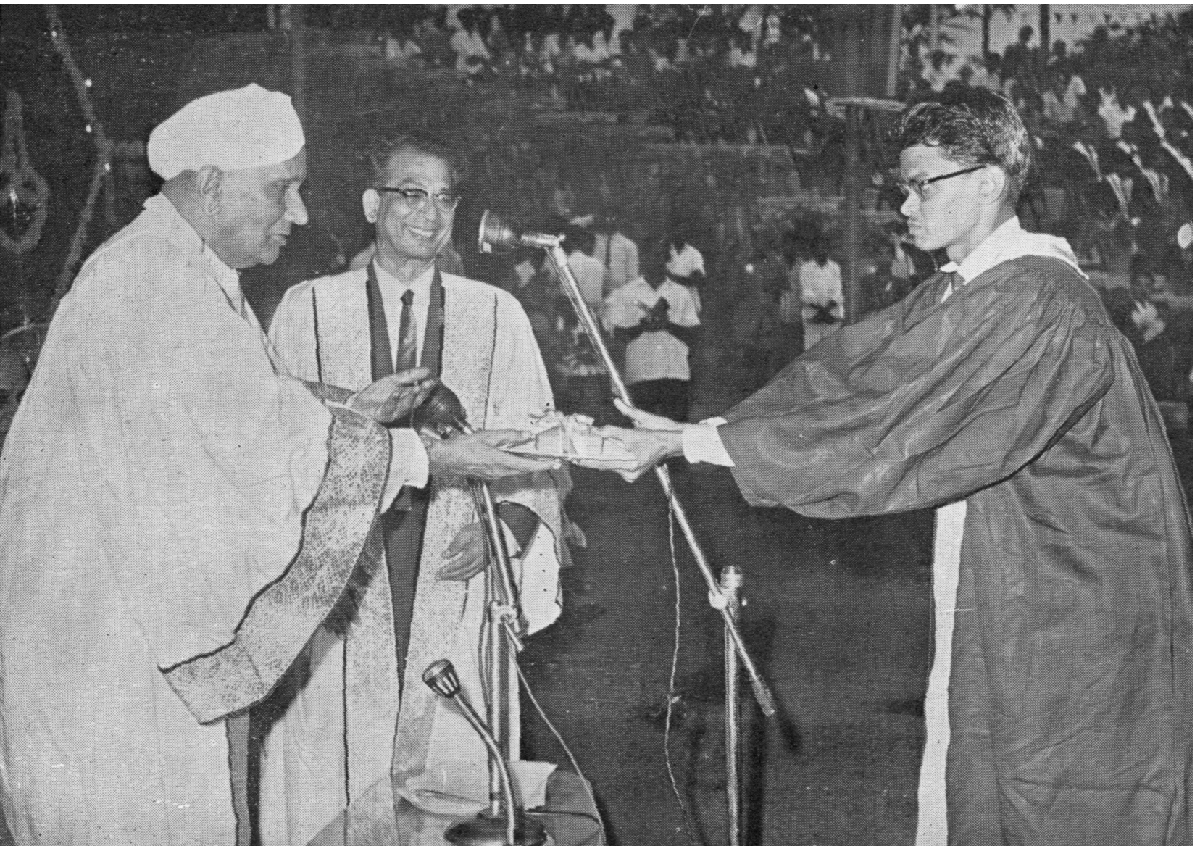
\includegraphics[scale=0.2]{"images/15.jpg"}
\caption{ರಾಮನ್‍ರವರು ಐಐಟಿ ಘಟಿಕೋತ್ಸವದಲ್ಲಿ ಡಿಪ್ಲೋಮಾ ಪತ್ರ ನೀಡುತ್ತಿರುವುದು}\label{chap4-fig02}
\end{figure}

ಸಾಮಾನ್ಯವಾಗಿ ತಂತ್ರಜ್ಞಾನ ಮತ್ತು ಉದ್ಯಮಗಳ ಜೊತೆಗೆ ಧೂಮ, ದೂಳು, ಕುರೂಪ, ಕಸ ಮತ್ತು ಇನ್ನೆಲ್ಲಾ ಕೆಟ್ಟ ಅಂಶಗಳೂ ಬೆಸೆದಿರುತ್ತವೆ. ಇವು ಹೀಗಿರಬೇಕಾಗಿಲ್ಲ. ನನ್ನ ಯುವ ಸ್ನೇಹಿತರೇ ಜೀವನವು ಆಹಾರ, ಬಟ್ಟೆ ಮತ್ತು ವಸತಿ ಪಡೆಯುವುದಕ್ಕಷ್ಟೇ ಸೀಮಿತವಾದರೆ, ನಿಮ್ಮ ಶಿಕ್ಷಣ ಅಪೂರ್ಣವೆನಿಸುತ್ತದೆ. ಮಾನವನು ಆಹಾರವೊಂದರಲ್ಲೇ ಜೀವನ ಸಾಗಿಸಲಾಗುವುದಿಲ್ಲ. ಇದು ಅನಾದಿಕಾಲದಿಂದಲೂ ತಿಳಿದದ್ದೇ. ಬದಲಿಗೆ ಸಂಗೀತ, ಹೂಗಳು, ಸೌಂದರ್ಯಪ್ರಜ್ಞೆ ಮತ್ತು ಇವುಗಳಿಂದ ಹೊಮ್ಮುವ ಆತ್ಮ ತೃಪ್ತಿಗಳು ಜೀವನಾವಶ್ಯಗಳು. ಇವೆಲ್ಲ ಜೀವನದ ಭವ್ಯ ಅಂಶಗಳು. ಮದರಾಸಿನ ಮಟ್ಟಿಗೆ ನಾವು ಸಂಗೀತಕ್ಕೆ ಪರದಾಡಬೇಕಾಗಿಲ್ಲ. ನೀವೆಲ್ಲಾ ಸಂಗೀತಾಸಕ್ತರೇ, ಹೀಗೆ ಇಲ್ಲದಿದ್ದರೆ ನಿಮ್ಮ ಬಗ್ಗೆ ಅನುಕಂಪ ಮೂಡುತ್ತದೆ. ಇಂತಹ ಸೂಕ್ಷ್ಮ ಅಂಶಗಳು ಜೀವನವನ್ನು ಸೊಗಸು ಮಾಡುತ್ತವೆ. ಜೀವನವನ್ನು ಸಾಗಿಸಲು ಮೌಲ್ಯ ನೀಡುತ್ತವೆ.

ಕೇಂದ್ರ ಸರ್ಕಾರ ಮತ್ತು ರಾಜ್ಯ ಸರ್ಕಾರಗಳ ಕೃಪೆಯಿಂದ ನೀವು ಈ ಸುಂದರ ವಾತಾವರಣದಲ್ಲಿ, ಭರ್ಜರಿ ವಿದ್ಯಾರ್ಥಿನಿಲಯಗಳಲ್ಲಿ, ಉತ್ತಮ ಪ್ರಯೋಗಾಲಯಗಳಲ್ಲಿ ಎಲ್ಲಕ್ಕಿಂತಲೂ ಮಿಗಿಲಾಗಿ ಗಿಡಗಳು ತುಂಬಿದ ಪರಿಸರದಲ್ಲಿ ಶುದ್ಧಗಾಳಿಯಲ್ಲಿ ಜೀವಿಸುತ್ತಿದ್ದೀರಿ. ಇದು ಜರ್ಮನ್ ದೇಶವಂತೂ ಅಲ್ಲ. (ಸೂಚನೆ: ರಾಮನ್ ಹೀಗೆ ಹೇಳಿದ್ದು ಏಕೆಂದರೆ\enginline{-} ಮದರಾಸಿಗೆ ಐಐಟಿ ಜರ್ಮನಿಯ ಸಹಾಯ ಒದಗಿತ್ತು. ಅಂದು ಜರ್ಮನಿಯಿಂದ ಅಧ್ಯಾಪಕರು ಬರುತ್ತಿದ್ದರು.) ಇಂತಹ ವಾತಾವರಣದಲ್ಲಿ ನಿಮಗೆ ಕ್ಷಯರೋಗವಂತೂ ಬರಲು ಸಾಧ್ಯವಿಲ್ಲ. ಇಲ್ಲಿ ನನಗೆ ಹಸ್ತಲಾಘವ ನೀಡಿದ ಮಹನೀಯ\-ರಿದ್ದಾರೆ. ಇವರಿಗೆ ನಾನು ಹಸ್ತಲಾಘವ ನೀಡಿದ್ದು ನನ್ನ ಸುಯೋಗವೆಂದೇ ತಿಳಿದ್ದಿದ್ದೇನೆ. ನಾನು ಎಲ್ಲಾ ಪದವೀಧರರಿಗೂ ಹಸ್ತ ಚಾಚಿದ್ದಾದರೆ ನನ್ನ ಕೈಗಳು ಸೋತುಹೊಗುತ್ತವೆ. ಸದೃಢ ಯುವಕರ ಹಸ್ತಗಳು ಬಲು ಗಟ್ಟಿ. ಇದು ಹೀಗೆಯೇ ಇರಬೇಕು. ಒಂದು ಭಾರವಾದ ಸುತ್ತಿಗೆಯನ್ನು ಎತ್ತಲಾರರಿಯೆಂದರೆ ಇಂಜೀನಿಯರಾಗಿ ಪ್ರಯೋಜನವೇನು? ದೇಹ ದಾರ್ಡ್ಯತೆ ಇಂಜೀನಿಯರಿಂಗ್‍ನ ಮೊದಲ ಆವಶ್ಯಕತೆ. ಹಾಗಾಗಿ ನಿಮ್ಮನ್ನು ನೋಡಿದಾಗ ನಿಮ್ಮ ದೇಹವನ್ನು ಚೆನ್ನಾಗಿ ನೋಡಿಕೊಂಡಿದ್ದೀರಿ ಎಂದು ಅನ್ನಿಸುತ್ತದೆ.


\heading{ಜರ್ಮನರ ಕೊಡುಗೆ}

ನಾನಿಲ್ಲಿ ಜರ್ಮನ್ ದೇಶದ ಬಗ್ಗೆ ಕೊಂಚ ಹೇಳುವುದು ಒಳಿತು. ನಿಮ್ಮ ಸಂಸ್ಥೆಯು ಒಳ್ಳೆಯ ಶಿಕ್ಷಣ ನೀಡುವಂತಾಗಲು ಈ ದೇಶವು ಬಹಳಷ್ಟು ಸಹಾಯ ಮಾಡಿದೆ. ಜರ್ಮನಿ ಎಂದರೆ ನನಗೆ ಭೂಪಟದ ನೆನಪು ಬರುವುದಿಲ್ಲ. ಜರ್ಮನಿ ಎಂದರೆ ಆ ದೇಶವನ್ನು ಕಟ್ಟಿದ ಧೀಮಂತರ ನೆನಪು ಬರುತ್ತದೆ. ನಾನು ಅನೇಕ ಹೆಸರುಗಳನ್ನು ಹೇಳಬಲ್ಲೆ. ಆದರೆ ನಾನು ಇಬ್ಬರನ್ನು ನೆನಸುತ್ತೇನೆ. ಇವರು ಜಗತ್ತು ಕಂಡ ಅತೀ ಶ್ರೇಷ್ಠ ತತ್ತ್ವಜ್ಞರು ಮತ್ತು ವಿಜ್ಞಾನಿಗಳು. \enginline{19} ನೇ ಶತಮಾನದ ಹರ್ಮನ್ ವಾನ್ ಹೆಲ್ಮ್ ‍ಹೋಲ್ಟ್ಸ್ ಮತ್ತು ಈಗಿನ ಆಲ್ಬರ್ಟ್ ಐನ್ಸ್ಟೈನ್. ಇವರಲ್ಲದೆ ಅನೇಕರೂ ಇದ್ದಾರೆ. ತಮ್ಮ ತಮ್ಮ ಹೆಸರನ್ನು ದಾಖಲಿಸಿದ್ದಾರೆ. ಜರ್ಮನಿ ಎಂದರೆ ಆ ದೇಶಕ್ಕೆ ಏನಾಗಿದೆ ಎಂಬುದಲ್ಲ ಜರ್ಮನಿ ಎಂದರೆ ಈ ಧೀಮಂತರೇ ನನ್ನ ಮನಸ್ಸಿಗೆ ಬರುತ್ತಾರೆ. ದೇಶವು ಚಿಕ್ಕದೆನಿಸಿದರೂ ಕೀರ್ತಿಯಲ್ಲಿ ಹಿರಿದಾದ ಜರ್ಮನಿಯ ಪ್ರಸಿದ್ಧ ಸ್ಥಳಗಳಿಗೆ ಭೇಟಿಕೊಡಬೇಕೆಂದು ನನ್ನ ಅಭೀಪ್ಸೆ. ಹೈಡೆಲ್ ಬರ್ಗ್, ಗಾಟಿಂಜನ್, ಮರ್ ಬರ್ಗ್, ಮುಂತಾದ ಊರುಗಳಿಗೆ. ನನಗೆ ಈ ಅದೃಷ್ಟ ದೊರಕುವುದು ಈಗ ದುಸ್ತರವೆ.

ಆದರೆ ದಶಕದ ಹಿಂದೆ ನನಗೆ ಲಾಂಡೋ ಪಟ್ಟಣಕ್ಕೆ ಆಹ್ವಾನ ಬಂದಿತ್ತು. ನಾನು ಇದು ನನಗೊದಗಿದ ಸುವರ್ಣಾವಕಾಶವೆಂದೇ ತಿಳಿದೆ. ನಾನಲ್ಲಿಗೆ ಹೋದೆ. ಲಾಂಡೋ ಬಹಳ ವಿಚಿತ್ರ ಸ್ಥಳವೆನಿಸಿತು. ಅದೆಷ್ಟು ವಿಚಿತ್ರವೆನಿಸಿತೆಂದು ನಾನಿಲ್ಲಿ ಹೇಳುವುದಿಲ್ಲ. ಈ ಪಟ್ಟಣವು ಕ್ಯಾನ್ಸ್ಟನ್ಸ್ ಎಂದು ಕರೆಯುವ ನದಿಯ ದಡದಲ್ಲಿದೆ. ಜರ್ಮನ್ನರು ಇದಕ್ಕೆ ಬೊಡೆನ್ಸೀ ಎಂದೂ ಕರೆಯುತ್ತಾರೆ. ಇದು ಸರಿಯಾದ ಉಚ್ಚಾರಣೆಯೇ ಎಂಬುದು ತಿಳಿದಿಲ್ಲ. ಅದು ಜರ್ಮನ್ ಸಾಮ್ರಾಜ್ಯದ ಸುಂದರ ಊರು. ಅದಕ್ಕೊದಗಿದ ವಿಶೇಷ ಸ್ವಾತಂತ್ರ್ಯವೆಂದರೆ ಅಲ್ಲಿನ ಕ್ಯಾಸಿನೋ\enginline{-}ಎಂದರೆ ಜೂಜಾಡುವ ಸ್ಥಳ. ಇದು ವಿಶೇಷ ಸ್ವಾತಂತ್ರ್ಯವೆನಿಸದಿದ್ದರೂ ಜನರು ಅಲ್ಲಿ ಜೂಜಾಡಿ ಹಣ ಸಂಪಾದಿಸುತ್ತಿದ್ದರು. ಈಗಲೂ ಅಲ್ಲಿ ಜೂಜಿದೆ. ಜನ ಹಣ ಮಾಡುತ್ತಿದ್ದಾರೆ. ಜೂಜಿನ ಕಟ್ಟೆಗೆ ಹೋಗುವವರೆಲ್ಲಾ ಹಣ ಮಾಡುತ್ತಾರೆಂದು ಜನ ತಿಳಿಯುತ್ತಾರೆ. ಹಾಗೇನೂ ಇಲ್ಲ. ಜೂಜಿನ ಕಟ್ಟೆ ನಡೆಸುವವನು ಮಾತ್ರ ಹಣ ಮಾಡುತ್ತಾನೆ ಅಷ್ಟೇ. ಹೀಗೆ ಲಾಂಡೋ ಪಟ್ಟಣವು ಸಾಕಷ್ಟು ಹಣ ಮಾಡಿತು. ಅಲ್ಲಿನ ಪುರಪಿತೃಗಳಿಗೆ ಈ ಹಣದಿಂದ ಏನೋ ಮುಜುಗರ. ಅದಕ್ಕೆ ಅವರು ತಮ್ಮ ಸಾಕ್ಷಿ ಪ್ರಜ್ಞೆಗೆ ಒಡಂಬಡಿಕೆ ಮಾಡಿಕೊಂಡರು. ಅವರು ಪ್ರತಿವರ್ಷ ಒಂದು ಸಮಾರಂಭ ಏರ್ಪಡಿಸುತ್ತಾರೆ ಅದಕ್ಕೆ ನೊಬೆಲ್ ಪುರಸ್ಕೃತರನ್ನೇ ಆಹ್ವಾನಿಸುತ್ತಾರೆ. ನೊಬೆಲ್ ಬಹಮಾನವೇ ಈ ಸಮಾರಂಭಕ್ಕೆ ಕನಿಷ್ಠ ಅರ್ಹತೆ. ಪ್ರತೀ ವರ್ಷವೂ ಇದು ಜರುಗುತ್ತದೆ. ಹೀಗೆ ದಶಕದ ಹಿಂದೆ ನನಗೆ ಆಹ್ವಾನ ಬಂದಿತ್ತು. ನಾನು ಹೋದೆ. ಅದು ಸುಂದರವಾದ ಊರು. ನಾನು ಹೋಗಲು ಮುಜುಗರವೆನಿಸಲಿಲ್ಲ. ಅಲ್ಲಿನ ಸರೋವರದ ನಡುವೆ ಒಂದು ದ್ವೀಪವಿದೆ. ಇದಕ್ಕೆ ಮೈನಾ ದ್ವೀಪವೆಂದು ಹೆಸರು. ಇದಕ್ಕೆ ವಾರಸುದಾರರು ಕೌಂಟ್ ಬರ್ನಾಡೊಟ್ಟೆ ಎಂಬುವವರು. ಅವರು ಸ್ವೀಡನ್‍ನ ರಾಜ ಕುಟುಂಬದಿಂದ ಬಂದವರು. ಅವರು ಈ ಸಮಾರಂಭ ಆತಿಥೇಯರಾಗಿದ್ದರು.

\vskip 2pt

ಇದಾದ ಮೇಲೆ ನಾನು ಅಲ್ಲಿ ಪುರಾತನ ವಿಶ್ವವಿದ್ಯಾಲಯವಾದ ಬ್ರೈಸ್ಗೋದಲ್ಲಿರುವ ಫೈಬರ್ಗ್‌ಗೆ ಹೋದೆ. ಅದು ನನಗೆ ಗೌರವ ಡಾಕ್ಟೊರೇಟ್ ನೀಡಿದ ಮೊದಲ ಯೂನಿವರ್ಸಿಟಿ. ಅಲ್ಲಿ ಒಂದು ವಾರವಿದ್ದು ಬಾನ್ ನಗರಕ್ಕೆ ತೆರಳಿದೆ. ಬಾನ್‍ನಿಂದ ಮ್ಯೂನಿಕ್‍ಗೆ ಬಂದು ಜರ್ಮನಿಯಿಂದ ಹೊರಬಿದ್ದೆ. ನಾನು ಬಾನ್ ನಲ್ಲಿದ್ದಿದ್ದು ಒಂದು ವಾರ ಮಾತ್ರ. ಆಗಿನ್ನೂ ಜರ್ಮನಿ ಇಸವಿ \enginline{1956}ರಲ್ಲಿಯೂ ಯುದ್ಧದ ಧ್ವಂಸದ ವಾತಾವರಣದಿಂದ ಹೊರಬಂದಿರಲಿಲ್ಲ. ಎಲ್ಲೆಡೆ ಮರು ನಿರ್ಮಾಣ ಕಾರ್ಯ ನಡೆಯುತ್ತಿತ್ತು. ಅಲ್ಲಿನ ಮ್ಯೂಸಿಯಂ ಆಫ್ ಮಿನಿರಾಲಜಿಯನ್ನು ನೋಡಿ ನಾನು ಬಹಳ ಪ್ರಭಾವಿತನಾದೆ. ಇದು ಬಾನ್ ನಗರದಲ್ಲಿದೆ. ಯುದ್ಧ ಸಂತ್ರಸ್ತ ದೇಶದಲ್ಲಿ ಅಂತಹ ಒಳ್ಳೆಯ ಮಾದರಿಗಳನ್ನು ಜೋಡಿಸಿಟ್ಟಿರುವುದು ನಂಬಲಿಕ್ಕೇ ಆಗಲಿಲ್ಲ. ಇದೊಂದು ನೆನಪಿಡಬೇಕಾದ ಸುಂದರ ವಿಷಯವಾಗಿತ್ತು. ಮಿಕ್ಕ ಅನುಭವಗಳನ್ನು ನಾನಿಲ್ಲಿ ಹೇಳುವುದಿಲ್ಲ.

\vskip 2pt

ಅಂದಿನ ಸಂದರ್ಭದಲ್ಲಿ ಹೀಗಾಯಿತು. ಇದುವರೆವಿಗೂ ಹೇಳಿದ್ದು ಪೀಠಿಕೆಯಾಗಿ. ನಮ್ಮ ದೇಶದ ಪ್ರಧಾನಿ ಜವಾಹರ ಲಾಲ್ ನೆಹರೂರವರು ಅಲ್ಲಿದ್ದರು. ನಾನಲ್ಲಿ ಇದ್ದದ್ದಕ್ಕಾಗಿ ಅವರಿದ್ದರೆಂದಲ್ಲ. ಇದೊಂದು ಆಕಸ್ಮಿಕ ಅಷ್ಟೆ. ಈ ಬಗೆಯ ಕಾಕತಾಳೀಯಗಳು ಆಗಾಗ್ಗೆ ಸಂಭವಿಸುತ್ತವೆ. ಅಲ್ಲಿನ ಭಾರತೀಯ ರಾಯಭಾರಿಯು ಜರ್ಮನಿ ದೇಶದ ಅಧ್ಯಕ್ಷರು ಕರೆದಿದ್ದ ಭೋಜನ ಕೂಟಕ್ಕೆ ನನ್ನನ್ನೂ ಆಹ್ವಾನಿಸಿದ್ದರು. ಟೇಬಲ್‍ನ ಸುತ್ತ ಅಧ್ಯಕ್ಷರು, ಜವಾಹರ ಲಾಲ್ ನೆಹರೂರವರು, ರಾಯಭಾರಿಗಳು, ನಾನು, ಮತ್ತಿತರರು ಕುಳಿತೆವು. ಆ ಸಂದರ್ಭದಲ್ಲಿ ಅಲ್ಲಿನ ಅಧ್ಯಕ್ಷರು ಜರ್ಮನ್ ಭಾಷೆಯಲ್ಲಿ \enginline{10} ನಿಮಿಷ ಮಾತನಾಡಿದರು. ಒಡನೆಯೇ ದುಭಾಷಿಗಳು ಅಷ್ಟೇ ಅವಧಿಯಲ್ಲಿ ಇಂಗ್ಲೀಷ್ ಗೆ ತರ್ಜುಮೆ ಮಾಡಿ ಹೇಳಿದರು. ಅನಂತರ ನೆಹರೂರವರು \enginline{10} ನಿಮಿಷ ಉತ್ತರಿಸಿದರು. ಇದನ್ನು ಜರ್ಮನ್ ಭಾಷೆಗೆ ಭಾಷಾಂತರಿಸಿ ಹೇಳಲಾಯ್ತು. ಅವರುಗಳ ಭಾಷಣ ನನಗಿಲ್ಲಿ ನೆನಪಿಲ್ಲವೆಂದು ಹೇಳಲೇಬೇಕು. ಆದರೂ ಇಂತಹ ಸಂದರ್ಭಗಳ ಔಪಚಾರಿಕ ಭಾಷಣಗಳ ಹಾಗೇ ಇವೂ ಇದ್ದಿರಬೇಕು. ನಾನು ಇದನ್ನು ಏಕೆ ಹೇಳುತ್ತಿದ್ದೇನೆಂದರೆ ಅಂದಿನ ಔತಣ ಕೂಟದಲ್ಲಿಯೇ ನಿಮ್ಮ ಐಐಟಿ ಸಂಸ್ಥೆಗೆ ಜರ್ಮನಿಯ ನೆರವು ಕೋರಿಕೆಯ ಮಾತುಕತೆಯಾಗಿದ್ದು, ಈ ಹತ್ತು ವರ್ಷಗಳು ಹಿಂದಕ್ಕೆ ಸರಿದಿವೆ. ಇಲ್ಲಿನ ಕಾಡು ಪ್ರದೇಶದಲ್ಲಿ ಹಾವು, ಚೇಳುಗಳು ಹರಿದಾಡಿದ ಪ್ರದೇಶದಲ್ಲಿ ನಿಮ್ಮ ಐಐಟಿ ಸಂಸ್ಥೆಯು ಸುಂದರವಾಗಿ ಎದ್ದು ನಿಂತಿದೆ. ಎಷ್ಟೊಂದು ಪರಿಕರಗಳೂ, ಕಟ್ಟಡಗಳೂ ಸೇರಿ, ಇಡೀ ದೇಶದ ಜನ ಇಲ್ಲಿ ಕಲಿಯುವಂತಾಗಿದೆ. ನನ್ನ ಭಾಷಣಕ್ಕೆ ಎಷ್ಟೊಂದು ವರ್ಣರಂಜಿತ ಜನಸ್ತೋಮ ಬಂದಿದೆ. ನನಗಿದು ಸಂತೋಷದ ವಿಷಯ. ಏಕೆಂದರೆ ನಾನು ಬಣ್ಣಗಳನ್ನು ಇಷ್ಟಪಡುತ್ತೇನೆ. ಗಂಡಸರು ಗಾಢ ಬಣ್ಣಗಳನ್ನು ತೊಡಬಾರದೆಂಬ ಅಲಿಖಿತ ನಿಯಮವಿದೆ. ಹೆಂಗಸರು ಇದನ್ನು ತೊಡಬಹುದು, ಅವರು ತೊಡುತ್ತಾರೆ ಕೂಡಾ. ಇದಕ್ಕೆ ಒಂದು ಅಪವಾದವಿದೆ. ಘಟಿಕೋತ್ಸವ ಇಂತಹ ಒಂದು ಅಪವಾದ. ಇಲ್ಲಿ ಗಂಡಸರೂ ಕೂಡಾ ರೋಹಿತದ ಎಲ್ಲಾ ವರ್ಣಗಳಲ್ಲೂ ಕಾಣಿಸಿಕೊಳ್ಳಬಹುದು. ರೋಹಿತದಲ್ಲಿ ಕಾಣದ ಬಣ್ಣಗಳಲ್ಲಿ ಅವರು ಹೆಂಗಸರಿಗೆ ಆಕರ್ಷಿತವಾಗಲು ದುಸ್ತು ಬಳಸಬಹುದೆನ್ನಿ.


\heading{ಯುವಜನತೆ ಮತ್ತು ಹೊಸ ದೃಷ್ಟಿ}

ಇದೊಂದು ಆನಂದಮಯ ಸುಸಂದರ್ಭ. ಈ ಹಿರಿಯ ಸಮಾರಂಭದಲ್ಲಿ ನನ್ನ ಯುವ ಸ್ನೇಹಿತರೆಲ್ಲಾ ಸಂತೋಷ ಭರಿತರಾಗಿದ್ದಾರೆಂದೇ ಭಾವಿಸುತ್ತೇನೆ. ಅವರ ಜೀವನದಲ್ಲಿ ಇದು ವಿಶೇಷ ಸಂದರ್ಭವೆಂದು ಅವರಿಗೆ ಬಹುಕಾಲ ನೆನಪಿರುತ್ತದೆ. ನನ್ನ ಮನಸ್ಸು \enginline{60} ವರ್ಷಗಳ ಹಿಂದೆ ಓಡುತ್ತದೆ. \enginline{60} ವರ್ಷಗಳ ಹಿಂದೆ ಇದೇ ಪಟ್ಟಣದಲ್ಲಿ ನಾನು ಹೀಗೆಯೇ ಪದವೀಧರನಾಗಿ ನನ್ನ ಜೇಬಿನಲ್ಲಿ ಇನ್ನೂ ಕೆಲವನ್ನು ಇಟ್ಟುಕೊಂಡು (ಅದೇನೆಂದು ಹೇಳಲಾರೆ) ಹೊರ ಬಂದೆ. ಆ ಘಟನೆಯು ನನಗೆ ಪ್ರಮುಖವಾಗಿ ಕಾಣುತ್ತಿದೆ. ನಾನದನ್ನು ಹೇಳಬೇಕು. ನಾನು ಹಿಂತಿರುಗಿ ನೋಡಿದಾಗ ನನಗೆ ಆಶ್ಚರ್ಯವಾಗುತ್ತಿದೆ. ನಾನು ಆ ನಾಲ್ಕು ವರ್ಷಗಳಲ್ಲಿ ಪಡೆದುಕೊಂಡ ಅನುಭವಗಳು, ನನ್ನ \enginline{60} ವರ್ಷಗಳಲ್ಲಿ ಏನೆಲ್ಲಾ ಸಾಧಿಸಿದ್ದೇನೋ ಅವುಗಳಿಂದ ಮಾಸಿಹೋಗಿಲ್ಲ. ಇದಕ್ಕಿಂತಲೂ ಆಶ್ಚರ್ಯಕರ ಸಂಗತಿಯೆಂದರೆ ಆ ನಾಲ್ಕು ವರ್ಷಗಳು, ನಾನು ಈ \enginline{60} ವರ್ಷಗಳಲ್ಲಿ ಮಾಡಿದ ಕಾರ್ಯವನ್ನು ಗಣಿತ ಸಮೀಕರಣದ ರೀತಿಯಲ್ಲಿ ನಿರ್ಧರಿಸಿದೆ. ನನಗೆ ಈ ನಾಲ್ಕು ವರ್ಷಗಳ ಅವಧಿಯಲ್ಲಿ ಸಿಕ್ಕ ಅವಕಾಶಗಳು ನನ್ನ ಮನಸ್ಸನ್ನು ಕೆಲವು ವಿಷಯಗಳಿಗೆ ಕೇಂದ್ರಿಕೃತಗೊಳಿಸಿಕೊಳ್ಳಲು ನೆರವಾದವು. ನಾನು ಈ ವಿಷಯಗಳಿಂದ ಇಂದೂ ವಿಮುಖನಾಗಲಾರೆ. ಏಕೆಂದರೆ ಅಂದಿನ ಯುವ ಉತ್ಸಾಹದ ಶಕ್ತಿ ಅಂತಹದು. ಪ್ರೆಸಿಡೆನ್ಸಿ ಕಾಲೇಜಿನೊಳಗೆ ಬಂದಾಗ ನನಗೆ \enginline{14} ವರ್ಷ. ಅಲ್ಲಿಂದ ಮಾಸ್ಟರ್ ಡಿಗ್ರಿ ಪಡೆದು ಹೊರಬಿದ್ದಾಗ \enginline{18} ವರ್ಷ. ಪದವಿ ಪಡೆದು ಹೊರಬಂದಾಗ ಹಣಕಾಸು ವಿಭಾಗದಲ್ಲಿ ಕೆಲಸ ಸಿಕ್ಕಿತ್ತು. ನನ್ನದೊಂದು ಸಂಶೋಧನಾ ಲೇಖನ ಪ್ರಕಟವಾಗಿ, ನನ್ನಲ್ಲಿನ ವಿಜ್ಞಾನಿಯ ಉದಯವಾಗಿತ್ತು. ಇವೆಲ್ಲವೂ ಆ ಹದಿನೆಂಟರ ಹರೆಯದಲ್ಲಿ. ಆ ಯುವ ವಯಸ್ಸಿನಲ್ಲಿ ಮನಸ್ಸಿಗೆ ವಿಷಯಗಳು ಚೆನ್ನಾಗಿ ನಾಟುತ್ತವೆ.

ನಾನಿದನ್ನು ನಿಮಗೆ ಒತ್ತಿ ಹೇಳಬೇಕಾಗಿದೆ. ಏಕೆಂದರೆ ಈ ನಾಲ್ಕು ಅಥವಾ ಐದು ವರ್ಷಗಳಲ್ಲಿ ನಿಮಗೆ ನುರಿತ ಅಧ್ಯಾಪಕರ ಸಂಪರ್ಕವಿರುತ್ತದೆ, ಹಾಗಯೇ ಹಳೆಯ ಆಲದ ಮರದ ಸಂಪರ್ಕವೂ ಇರುತ್ತದೆ. ಇದು ನಗಣ್ಯವೇನಲ್ಲ.

ಇವುಗಳ ಪ್ರಭಾವಗಳೆ ನಿಮ್ಮ ಭವಿಷ್ಯದ ವೃತ್ತಿಯನ್ನು ನಿರ್ಧರಿಸುತ್ತವೆ. ಅಷ್ಟೇ ಅಲ್ಲ ನೀವು ಏನಾಗಲಿದ್ದೀರಿ ಎಂಬುದು ನೀವು ಮುಂದಿನ ಕೆಲವು ವರ್ಷಗಳಲ್ಲಿ ಏನು ಮಾಡುತ್ತೀರಿ ಎಂಬುದರ ಮೇಲೆ ಅವಲಂಬಿತವಾಗಿದೆ. ನೋವಿನ ವಿಚಾರವೆಂದರೆ ಡಿಗ್ರಿಗಳನ್ನು ಸಂಪಾದಿಸಿದ ಮೇಲೆ, ಕೆಲಸಕ್ಕೆ ಸೇರಿ ಬಹುಶಃ ಮದುವೆಯಾಗಿ ಕಾಲೇಜಿನಲ್ಲಿ ಕಲಿತಿದ್ದೆಲ್ಲವನ್ನೂ ಮರೆತು ಬಿಡುತ್ತಾರೆ. ಹೀಗೆ ಮಾಡಬಾರದು. ನೀವು ಒಂದಿಷ್ಟು ಮೌಲ್ಯಯುತ ಜೀವನ ಸಾಗಿಸಬೇಕಾದರೆ, ಈ ನಾಲ್ಕೈದು ವರ್ಷಗಳಲ್ಲಿನ ನಿಮ್ಮ ಅನುಭವವೇ ತಳಹದಿಯಾಗಬೇಕಾಗುತ್ತದೆ. ಈ ತಳಹದಿಯ ಮೇಲೆಯೇ ನೀವು ಭವಿಷ್ಯ ನಿರ್ಮಿಸಿಕೊಳ್ಳಬೇಕಾಗಿದೆ.

ನಾನು ನಿಮಗೆ ನೆನಪಿಸಬೇಕಾದ್ದೆಂದರೆ, ನೀವು ಕೆಲವು ಸಂಗತಿಗಳನ್ನು ಮರೆಯಬಾರದು. ನಿಮ್ಮಲ್ಲಿರುವ ಅತ್ಯಮುಲ್ಯ ವಸ್ತುವೆಂದರೆ ಅದು ನಿಮ್ಮ ದೇಹ. ಇದು ಎಲ್ಲರಿಗೂ ಇದೆ. ಇದನ್ನು ನಮ್ಮ ಮಾತಾಪಿತೃಗಳು ನಮಗೆ ನೀಡಿದ್ದಾರೆ. ನಾನು ಇತ್ತೀಚಿನ ಅಧ್ಯಯನಗಳಲ್ಲಿ ಭೌತಶಾಸ್ತ್ರ, ರಸಾಯನಶಾಸ್ತ್ರ, ಖನಿಜಶಾಸ್ತ್ರ ಮತ್ತು ಗಣಿತಶಾಸ್ತ್ರಗಳನ್ನು ಕೈಬಿಟ್ಟು ಮಾನವನಿಗಿರುವ ಲಕ್ಷಣಗಳ ಬಗ್ಗೆ ನನ್ನ ಗಮನವನ್ನು ತಿರುಗಿಸಿದ್ದೇನೆ. ಇವುಗಳಲ್ಲಿ ಕೆಲವು ನಮ್ಮ ಗೋಚರಕ್ಕೆ ಬರುವುದಿಲ್ಲ. ನಾವದರ ಇರುವಿಕೆಯನ್ನು ಯೋಚಿಸದೆಯೇ ಒಪ್ಪಿ ಬಿಡುತ್ತೇವೆ, ಈ ಬಗೆಯ ಶರೀರ ಅಧ್ಯಯನವನ್ನು ಕೈಗೆತ್ತಿಕೊಂಡಾಗಿನಿಂದ ನಮ್ಮಲ್ಲಿ ಎಂತಹ ಶ್ರೇಷ್ಠ ದಾಸ್ತಾನು ಇದೆ ಎಂದು ಚಕಿತಗೊಂಡಿದ್ದೇನೆ.

ಇನ್ನೊಂದು ಸಣ್ಣ ವಿಷಯವನ್ನು ನಾವೆಲ್ಲರೂ ಮರೆತು ಬಿಡುತ್ತೇವೆ. ಈ ಸಣ್ಣದನ್ನು ‘ಹೃದಯ’ ಎನ್ನುತ್ತಾರೆ. ನೀವು ಹುಟ್ಟಿದ ತಕ್ಷಣ ಇದು ಕೆಲಸಮಾಡಲು ಶುರು ಮಾಡುತ್ತದೆ. ಅಥವಾ ಹುಟ್ಟುವ ಮೊದಲೇ ತನ್ನ ಕೆಲಸ ಆರಂಭಿಸಿರುತ್ತದೆ. ಟಿಕಿ, ಟಿಕಿ ಶಬ್ದದೊಡನೆ ನೀವು ಯುವಕರಾದಾಗಲೂ ಇರುತ್ತದೆ. ನಿಮಗೆ ವಯಸ್ಸಾಗತೊಡಗಿದಂತೆ ಒಂದೇ ಸಮನೆ ಟಿಕಿ ಟಿಕಿ ಸದ್ದಿನೊಡನೆ ಸಾಯುವವರೆಗೂ ನಿಮ್ಮೊಡನೆ ಇರುತ್ತದೆ. ಟಿಕಿ ಟಿಕಿ ಶಬ್ದವಿಲ್ಲದಾಗ ನೀವು ಸತ್ತಂತೆಯೇ. ಈ ಯಂತ್ರವನ್ನು ನನ್ನ ಯುವ ಸ್ನೇಹಿತರೇ \enginline{-} ‘ನೀವು ಕಾಪಾಡಿಕೊಳ್ಳಬೇಕು. ಬಹಳ ಹಿರಿಯ ವ್ಯಕ್ತಿಗಳು ಅಚಾನಕ್ಕಾಗಿ ಕುಸಿದು ಬೀಳುವುದನ್ನು ನೀವು ನೋಡಿರುತ್ತೀರಿ. ಅವರ ಡಾಕ್ಟರರು ಇದಕ್ಕೆ ಹೃದಯ ಸ್ಥಂಬನವೆನ್ನುತ್ತಾರೆ. ಹೃದಯ ನಿಂತು ಜನ ಸಾಯುತ್ತಾರೆ. ಇದು ಏಕೆ ಹೀಗಾಗುತ್ತದೆ? ಏಕೆಂದರೆ ಅವರು ಈ ಸಣ್ಣಯಂತ್ರವನ್ನು ವಿಪರೀತ ದುಡಿಸಿರುತ್ತಾರೆ. ಅವರ ದೇಹವನ್ನೂ ಅಪವ್ಯಯ ಗೊಳಿಸಿಕೊಂಡಿರುತ್ತಾರೆ. ನಾನು ಯುವಕನಾಗಿದ್ದೇನೆ, ನಾನು ಏನು ಬೇಕಾದರೂ ಮಾಡಬಲ್ಲೆ ಎಂದುಕೊಳ್ಳುತ್ತಾರೆ.\break ಮೆಣಸಿನಕಾಯಿ ತಿಂದು, ರಾತ್ರಿಯಿಡೀ ಥಿಯೇಟರಿನಲ್ಲಿ ಕುಳಿತು, ಸ್ನೇಹಿತರೊಡನೆ ಪಾರ್ಟಿಗಳನ್ನು ಮಾಡುವುದೇ ಖುಷಿ ಎಂದು ಕೊಳ್ಳುತ್ತಾರೆ. ಆ ವಯಸ್ಸಿನಲ್ಲಿ ದೇಹವು ತಡೆದುಕೊಳ್ಳಬಲ್ಲದು. ಇದರ ಬಳಿಕ ಏನಾಗುತ್ತದೆ? ನಿಮಗೆ ಬಲು ಬೇಗನೆ ವೃದ್ಧಾಪ್ಯ ಅಂಟುತ್ತದೆ. ಹೃದಯ ಬೇನೆ ಆವರಿಸುತ್ತದೆ. ನಿಮ್ಮನ್ನು ಕೊಂಡೊಯ್ಯುತ್ತದೆ. ನೀವು ಯುವಕರಾಗಿದ್ದಾಗಲೇ ಇದನ್ನು ತಿಳಿದುಕೊಳ್ಳಿ ಎಂದು ಆಶಿಸುತ್ತೇನೆ. ನಾನು ಅನುಷ್ಠಾನಗೊಳಿಸಲಾಗದ್ದನ್ನು ನಿಮಗೆ ಉಪದೇಶ ಮಾಡುತ್ತಿದ್ದೇನೆ ಎಂದು ಕೊಳ್ಳಬೇಡಿ. ನಾನು ಇದನ್ನೆಲ್ಲಾ ಅನುಸರಿಸಿದ್ದೇನೆ, ನಾನು ಉಪದೇಶದಲ್ಲಲ್ಲ \enginline{-} ಆಚರಣೆಯಲ್ಲಿ ನಂಬಿಕೆ ಇರಿಸಿದ್ದೇನೆ. ಒಬ್ಬ ಉತ್ತಮ ಶಿಕ್ಷಕನು ತನ್ನ ಉದಾಹರಣೆಯಿಂದ ಮಾತ್ರವೇ ಶಿಕ್ಷಣ ನೀಡಬಲ್ಲ. ಉಪದೇಶದಿಂದಲ್ಲ. ಈಗ ನಿಮ್ಮಲ್ಲಿ ಬಿಸಿ ರಕ್ತ ಹರಿಯುತ್ತಿದೆ. ನೀವು ಯುವ ಉತ್ಸಾಹದಿಂದ ಇದ್ದೀರಿ. ನೀವು ಇಲ್ಲಿ ಕಲಿತಿದ್ದದ್ದರಲ್ಲಿ ಹೆಚ್ಚಿನ ಸಾಧನೆ ಮಾಡಬೇಕಾಗಿದೆ.

ಭಾರತ ದೇಶದಲ್ಲಿ ಜನಸಂಖ್ಯೆ ಅತಿಹೆಚ್ಚು. ನಾವೆಲ್ಲ ನಮ್ಮ ದೇಶವನ್ನು ಭವ್ಯವಾಗಿಸಲು ಹೊರಟಿದ್ದೇವೆ. ಆದರೆ ಇದಕ್ಕೆ ದುಡಿಯುವವರಾರು? ದೇಶದ ಬುದ್ಧಿವಂತ ಯುವ ಜನತೆ ಮಾತ್ರ. ಅವರ ದುಡಿಯುವ ಕೈಗಳನ್ನೇ ಅಲ್ಲದೆ ಅವರ ಮೆದುಳನ್ನೂ ಉಪಯೋಗಿಸಲು ಕಲಿಯ ಬೇಕಿದೆ. ಜೀವನದ ಎಲ್ಲ ಸಮಸ್ಯೆಗಳಿಗೆ ಸ್ವತಂತ್ರ ಆಲೋಚನೆ ಮಾಡಬೇಕಾಗಿದೆ. ನಿಮಗೆ ಜೀವನದಲ್ಲಿ ತೀವ್ರತೆ ಇರಬೇಕು. ನೀವು ಸಣ್ಣಪುಟ್ಟ ಖುಷಿ ಕೊಡುವ ವಿಚಾರಗಳೂ, ಆತುರದ ಆನಂದಗಳೂ ನಿಮಗೆ ಸಹಾಯ ಮಾಡುತ್ತವೆಂದು ತಿಳಿದು ಕುಳಿತುಕೊಳ್ಳಬಾರದು. ವಿಜ್ಞಾನ ಚಟುವಟಿಕೆಗಳಲ್ಲಿ ನಿರತವಾಗಿ ನಾನು ಕಳೆದ \enginline{60} ವರ್ಷಗಳಲ್ಲಿ ಕಲಿತಿದ್ದು ಇದೇ. ಸಾಧನೆಯೇ ಮನುಷ್ಯನಿಗೆ ನಿಜವಾದ ಆನಂದ ತರುವ ವಿಷಯ. ಏನಾದರೂ ಮೌಲ್ಯಯುತ ಸಾಧನೆಗೈದರೆ ಮಾತ್ರ ಜಗತ್ತು ಗುರುತಿಸುತ್ತದೆ. ರಿಸರ್ವ್ ಬ್ಯಾಂಕ್ ನಲ್ಲಿ ನೀವು ನೋಡುವ ಹಣದ ಚೀಲಗಳು ನಿಮ್ಮ ಸಾಧನೆಯ ಮುಂದೆ ಗೌಣವಾಗುತ್ತವೆ. ಸಾಧನೆಯ ಆನಂದವೇ ಹಿರಿದಾದುದು. ವಿಶ್ವವಿದ್ಯಾನಿಲಯಗಳಿಂದ ಹೊರ ಬರುವ ಯುವಕರು ಅವರಿಗೆ ಯಾವುದು ಸಂತೋಷವುಂಟು ಮಾಡುತ್ತದೆ ಎಂದೂ, ಮತ್ತು ಅವರು ಭೌತಿಕ ಸಂಪತ್ತನ್ನು ಗಳಿಸುವ ಬಗೆ ಯಾವುದು ಎಂದೂ ಮತ್ತು ದೇಶಕ್ಕೆ ಖ್ಯಾತಿ ತರುವುದು ಹೇಗೆ ಎಂಬ ವಿಚಾರಗಳ ಬಗ್ಗೆಯೂ ಯೋಚಿಸುತ್ತಾರೆಂದು ತಿಳಿದಿದ್ದೇನೆ. ಯುವಕರಾಗಿದ್ದಾಗ ಈ ಆಲೋಚನೆಗಳು ಬಂದರೆ ಮಾತ್ರ ಅವರು ಇವನ್ನು ಸಾಧಿಸಬಲ್ಲರು.

ನಾನು ಯೌವನ ಮತ್ತು ವೃದ್ಧಾಪ್ಯಗಳ ಬಗ್ಗೆ ಒಂದು ಸಂಶೋಧನೆಯನ್ನೇ ಮಾಡಬಲ್ಲೆ. “ವಯಸ್ಸು ಮತ್ತು ಯೌವನ” ಎಂಬ ವಿಷಯದ ಬಗ್ಗೆ ಅರ್ಧಗಂಟೆ ಮಾತನಾಡಬಲ್ಲೆ. ಮುಗಿದ ವಯಸ್ಸನ್ನು ಬುದ್ಧಿವಂತಿಕೆಯೊಡನೆ ಜೋಡಿಸುತ್ತಾರೆಂಬುದು ನಿಮಗೆ ಗೊತ್ತಿದೆ. ಆದರೆ ಹಿರಿಯರು ಏನಾದರೂ ತಿಳಿದುಕೊಳ್ಳಲಿ ನಾನು ಇದನ್ನು ಪ್ರಶ್ನಿಸುತ್ತೇನೆ. ಯೌವನವು ಅದರ ಜೊತೆಗೆ ಏನನ್ನು ಹೊತ್ತು ತರುತ್ತದೆಂದು ನಾನು ಹೇಳುತ್ತೇನೆ. ನೀವು ಯೌವನದಲ್ಲಿ ನಿಮ್ಮನ್ನು ನೀವು ಸರಿಯಾಗಿ ನೋಡಿಕೊಳ್ಳದಿದ್ದರೆ, ನಿಮ್ಮ ಹಲ್ಲು ಉದುರುತ್ತದೆ, ಮೂಳೆ ಸವೆಯುತ್ತದೆ, ಕಣ್ಣು ಮಂಜಾಗುತ್ತದೆ, ಕಿವಿ ಮಂದವಾಗುತ್ತದೆ ಇದಕ್ಕಿಂತಲೂ ದುರಂತವೆಂದರೆ ನೀವು ಇತರರನ್ನು ಅಸಡ್ಡೆಯಿಂದ ಕಾಣುವಿರಿ, ನೀವು ಸಿನಿಕರಾಗುವಿರಿ. ನೀವು ಯಾವ ಮಟ್ಟಕ್ಕೆ ಕುಸಿಯುತ್ತೀರೆಂದರೆ, ಬದುಕಲೇ ಬೇಕೆಂಬ ತೆವಲು ಇಲ್ಲದೇ ಹೋದರೆ, ಮಾರ್ಫಿನ್ ನುಂಗಿ ಜೀವ ಕಳೆದು ಕೊಳ್ಳಲು ಸಿದ್ಧರಾಗುವಿರಿ. ಹೆಚ್ಚಿನಂಶ ಇದನ್ನು ಯಾರೂ ಮಾಡಲು ಹೋಗುವುದಿಲ್ಲ. ಏಕೆಂದರೆ ದೇವರು ಯಾವುದೇ ಕಷ್ಟ ಬಂದರೂ ಎಲ್ಲರಿಗೂ ಬದುಕಿ ಮುನ್ನಡೆಯುದ ಛಲ ನೀಡಿದ್ದಾನೆ. ನಾನಿದನ್ನು ನಿಮಗೇಕೆ ಹೇಳುತ್ತಿದ್ದೇನೆಂದರೆ, ವೃದ್ಧಾಪ್ಯದಲ್ಲಿ ಉತ್ಸಾಹ, ಆಸೆಗಳು, ಸಾಧನೆ ಗೈಯಲು ಉದ್ದೇಶ, ಕೆಲಸ ಮಾಡಲು ಶಕ್ತಿ ಮುಂತಾದುವನ್ನು ಕ್ರೋಡಿಕರಿಸಿಕೊಳ್ಳುವುದೇ ದುಸ್ತರವಾಗುತ್ತದೆ. ಯೌವನವೇ ಜೀವನದ ಅತಿ ಭವ್ಯ ಕಾಲಾವಧಿ. ವಿಜ್ಞಾನದ ಅತ್ಯದ್ಭುತ ಆವಿಷ್ಕಾರಗಳನ್ನು ಯುವಕರೇ ಮಾಡಿದ್ದಾರೆ. ಆವಿಷ್ಕಾರಗಳು ಹೊರಬರಲು ಯುವ ಉತ್ಸಾಹವೂ, ಏನಾದರೂ ಸಾಧನೆ ಮಾಡಲೆಂಬ ಹಠವೂ, ಹೊಸದೃಷ್ಟಿಕೋನವೂ\break ಬೇಕಾಗುತ್ತದೆಯೇ ಹೊರತು, ವೃದ್ಧಾಪ್ಯದಿಂದ ಬರುವ ಜಾಣತನದಿಂದಲ್ಲ. ಇವೇ ಜೀವನವನ್ನು ಮೌಲ್ಯಯುತವಾಗಿಸುವುದು. ನೀವಿದನ್ನು ತಿಳಿಯಬೇಕು. ನಾನು ಇನ್ನೂ ಯುವಕನಾಗಿದ್ದೇನೆ. ನನ್ನಲ್ಲಿ ಯೌವನೋತ್ಸಾಹವಿದೆ. ನನ್ನ ಕೈಯಲ್ಲಿ ಏನು ಸಾಧ್ಯವೋ ನೋಡೋಣ ಎಂದುಕೊಂಡಾಗ ಮಾತ್ರವೇ ಆವಿಷ್ಕಾರಗಳು ಸಾಧ್ಯವಾಗುತ್ತವೆ.


\heading{ಸ್ವತಂತ್ರ ಆಲೋಚನೆ ಮತ್ತು ನಿರ್ಭಯತೆ}

ಇದೆಲ್ಲಕ್ಕಿಂತ ಮಿಗಿಲಾಗಿ, ನನ್ನ ಸ್ವಂತ ಅನುಭವವೆಂದರೆ ಶತಮಾನಗಳಿಂದ ನಮ್ಮನ್ನು ಹೊರಗಿನಿಂದ ಬಂದ ಆಕ್ರಮಣಕಾರರು ತುಳಿದಿಟ್ಟಿದ್ದಾರೆ. ನಾನು ಇವರ ಪಟ್ಟಿಯನ್ನು ಹೇಳಲು ಇಚ್ಛಿಸುವುದಿಲ್ಲ. ಈ ಪರಿಣಾಮದಿಂದ, ನಮ್ಮ ತಲೆಗೆ ತುಂಬಿರುವ ವಿಚಾರವೆಂದರೆ “ಕೀಳರಿಮೆ.” ನಾವು ಹೊರಗಿನಿಂದ ಬಂದವರನ್ನು ಅಥವಾ ಬಂದದ್ದನ್ನು ಪ್ರಶ್ನಿಸುವುದಿಲ್ಲ. ನಮಗೆ ಪಠ್ಯಪುಸ್ತಕವಾಗಿ ಬಂದಿದ್ದೆಲ್ಲಾ ನಿಜವೇ ಎನ್ನಿಸುತ್ತದೆ. ಯಾರೋ ಒಬ್ಬ ದೊಡ್ಡ ಮನುಷ್ಯ ಹೇಳಿದ್ದಾನೆಂದರೆ ಆಯಿತು, ಅವನಿಗೆ ಶಿರಸಾವಹಿಸಿ ಅವನ ಮುಂದೆ ನಡುಗುತ್ತ ನಿಲ್ಲುತ್ತೇವೆ. ಇದು ನಮ್ಮ ಮನಸ್ಸಿಗೆ ತಡೆಗೋಡೆಯಂತಾಗುತ್ತದೆ. ಅಂದರೆ ನೀವೆಲ್ಲ ನಮ್ಮ ಹಿರಿಯರನ್ನು ಅಗೌರವಿಸಿ, ಗರ್ವಿಷ್ಠರಾಗಿ ಎಂದು ಹೇಳುತ್ತಿಲ್ಲ. ನಾನು ನಿಮ್ಮ ಗಮನ ಸೆಳೆಯುತ್ತಿರುವುದು, ಯಾರೂ ಸಹ ಋಷಿಗಳಲ್ಲ. ಅಜೇಯರಲ್ಲ, ಹರ್ಮನ್ ವಾನ್ ಹೆಲ್ಮ್ ‍ಹೋಲ್ಟ್ಸ್ ಕೂಡ. ಐನ್‍ಸ್ಟೈನ್ ಸಹ ಯಾರೂ ಅಜೇಯರಲ್ಲ. ಹೊಸ ಜ್ಞಾನವು ಈವರೆಗೆ ಅರಿತಿದ್ದುದನ್ನೆಲ್ಲಾ ಹೊರಗೆಸೆಯಬಹುದು.

ಹಾಗಾಗಿ ನನ್ನ ಆಲೋಚನೆಯೆಂದರೆ, ನಾವು ಭಾರತೀಯರು ನಿರ್ಭಯರಾಗಿ ಯೋಚಿಸುವುದನ್ನು ಕಲಿಯಬೇಕು. ಈ ಲಕ್ಷಣ ನಮಗೆ ಅತ್ಯಂತ ಅವಶ್ಯ. ಇದಿಲ್ಲದಿದ್ದರೆ ನಾವು ಮುನ್ನಡೆಯುವುದು ಕಷ್ಟಸಾಧ್ಯ. ನಾವಿಂದು ಏನು ಮಾಡಬೇಕಾದರೂ ಹೊರಗಿನಿಂದ ಹಣವನ್ನು ಸಾಲ ತರುತ್ತೇವೆ. ನಾವು ನೂರು ಶತಕೋಟಿಗೂ ಹೆಚ್ಚು ಸಾಲ ಮಾಡಿದ್ದೇವೆ.

ನಮಗೆ ಈಗ ಬಂದಿರುವ ಸ್ವಾತಂತ್ರ್ಯ ಎಂತಹದು? ನಾನು ರಾಜಕೀಯ ವಿಷಯಕ್ಕೆ ಹೊರಳದೆ ಹೇಳುವುದಾದರೆ ಈಗ ನಮ್ಮನ್ನು ಸಾಲನೀಡಿದ ಹೊರರಾಷ್ಟ್ರಗಳ ಕೂಟವು ನಮ್ಮನ್ನು ಆಳುವಂತಾಗಿದೆ. ನಮ್ಮನ್ನು ನಾವು ಆಳಿಕೊಳ್ಳುತ್ತಿಲ್ಲ. ಇದನ್ನು ಪಕ್ಕಕ್ಕೆ ಇರಿಸಿದರೆ, ಹಣವನ್ನು ಸಾಲ ಪಡೆಯುವುದೇ ಸರಿಯಿಲ್ಲವೆನ್ನಿಸಬಹುದು. ಹೊರಗಿನಿಂದ ಜ್ಞಾನವನ್ನು ಆಮದು ಮಾಡಿಕೊಂಡರೆ, ನಮ್ಮಲ್ಲಿನ ಜ್ಞಾನದ ಕಥೆ ಏನು? ನಮ್ಮನ್ನು ನಾವು ಮರೆತರೆ? ಈ ಬಗೆಯ ಅಸಹಾಯಕತೆಯನ್ನು ಹೊರಗೆಸೆಯಬೇಕು. ಕರುಣೆಯಿಲ್ಲದಂತೆ ತೊಳೆದು ಹಾಕಬೇಕು. ನಮ್ಮ ಕಾಲ ಮೇಲೆ ನಾವು ನಿಲ್ಲಬೇಕೆಂಬುದು ನಮಗೆ ಅರಿವಾಗಬೇಕು. ನಮ್ಮಲ್ಲಿರುವ ಹಳೆಯ ಉಪಕರಣಗಳನ್ನು ಇಟ್ಟುಕೊಂಡೇ ಕೆಲಸಮಾಡುವುದು ಒಳಿತು. ಹೊರಗಿನಿಂದ ತರಿಸಿದ ಕೋಳಿ ಪುಕ್ಕವನ್ನು ಜುಟ್ಟಿಗೆ ಸಿಕ್ಕಿಸಿಕೊಳ್ಳುವ ಬದಲು, ನಮ್ಮಲ್ಲಿನ ಕನಿಷ್ಠ ಸವಲತ್ತುಗಳಲ್ಲೇ ಕೆಲಸಮಾಡಲು ತೊಡಗುವುದು ಒಳಿತು. ನಾವಿದನ್ನು ಮನವರಿಕೆ ಮಾಡಿಕೊಳ್ಳಬೇಕು. ಇದನ್ನು ಅರಿಯದಿದ್ದರೆ ಮುನ್ನಡೆ ಅಸಾಧ್ಯ. ನನ್ನ ಉದ್ಯಮಿ ಸ್ನೇಹಿತರು ಹೆಚ್ಚು ದುಡ್ಡುತೆತ್ತು ಹೊರಗಿನಿಂದ ತಂತ್ರಜ್ಞಾನವನ್ನು ದೇಶದ ಒಳಗೆ ತರಬೇಕೆಂದಿದ್ದಾರೆ. ಅವರು ಇದರಲ್ಲಿ ಉದ್ಧಾರವಾಗುವುದಿಲ್ಲವೆಂದು ಭರವಸೆ ನೀಡಬಲ್ಲೆ. ಅವರು ಮುಂದುವರಿಯು\-ವುದು ಸಾಧ್ಯವಿಲ್ಲ. ಇದರ ಲಕ್ಷಣಗಳು ಈಗಾಗಲೇ ಗೋಚರಿಸುತ್ತಿವೆ. ರೂಪಾಯಿಯ ಬೆಲೆ ಕುಸಿದಿದೆ. ಮಿನೂ ಮಸಾನಿಯವರು ಹೇಳುವಂತೆ (ಸೂಚನೆ: ಸ್ವತಂತ್ರ ಪಕ್ಷದ ನೇತಾರರು) ಈಗಿನ ವಿನಿಮಯ ಬೆಲೆ ಐದು ಸೆಂಟ್ ಗಳಿಗೆ ಇಳಿಯಲೂ ಬಹುದು. ಇದು ಹೀಗಾಗಬೇಕೆಂದು ನಾನು ಬಯಸುವುದಿಲ್ಲ.


\vskip 2pt

\heading{ವಿಜ್ಞಾನ ಮತ್ತು ತಂತ್ರಜ್ಞಾನಗಳ ಮುನ್ನಡೆ}

\vskip 2pt

ನೀವೆಲ್ಲ ಇಂಜಿನಿಯರುಗಳು. ಆದರೂ ನಾನಿಲ್ಲಿ ಇದನ್ನು ಹೇಳಬೇಕು. ನೈಜ ಜ್ಞಾನದ ತಳಹದಿಯಿಲ್ಲದಿದ್ದರೆ ಯಾವುದೇ ದೇಶವೂ ಔದ್ಯಮಿಕ ರಂಗದಲ್ಲಿ ಸಾಧನೆ ಮಾಡಲಾರದು. ವಿಜ್ಞಾನ ನಮಗೆ ಕಲಿಸಿದ ಪಾಠವಿದು. ವಿಜ್ಞಾನವು ಪದೇ ಪದೇ ಸಾಬೀತುಮಾಡಿರುವ ಅಂಶವೆಂದರೆ, ವಿಜ್ಞಾನ ಮೊದಲು ಹೆಜ್ಜೆಯಿಟ್ಟರೆ ಅದರ ಹಿಂದೆ ತಂತ್ರಜ್ಞಾನ ಅಡಿಯಿಡುತ್ತದೆ. ವಿಜ್ಞಾನವಿಲ್ಲದಿದ್ದರೆ ತಂತ್ರಜ್ಞಾನವಿಲ್ಲ. ಜರ್ಮನಿ ಏಕೆ ಅಷ್ಟೊಂದು ದೊಡ್ಡ ಸಾಧಕ ದೇಶವಾಗಿದೆ? ಏಕೆಂದರೆ \enginline{19}ನೇ ಶತಮಾನದಲ್ಲಿ ಜರ್ಮನಿಯಲ್ಲಿ ವಿಜ್ಞಾನದ ಪ್ರತಿಯೊಂದು ಶಾಖೆಯಲ್ಲಿಯೂ ಪ್ರಸಿದ್ಧ ವಿಜ್ಞಾನಿಗಳು ಹಿಂಡು ಹಿಂಡಾಗಿ ಬಂದು ಹೋದರು. ಅವರು ತಂತ್ರಜ್ಞರಲ್ಲ. ವಿಶ್ವವಿದ್ಯಾನಿಲಯಗಳಲ್ಲಿ ಸಾಮಾನ್ಯ ಶಿಕ್ಷಕರಷ್ಟೇ. ಆದರೆ ಅವರು ಜ್ಞಾನ ಪಿಪಾಸುಗಳು. ಅವರು ತಮ್ಮ ಶಿಷ್ಯರನ್ನು ಜ್ಞಾನದ ಅನ್ವೇಷಣೆಗೆ ಹಚ್ಚಿದರು. ಅವರು ವಿಜ್ಞಾನದ ಚಿಲುಮೆಯಂತಿದ್ದರು. ಈ ಚಿಲುಮೆಯೇ ನದಿಯಾಗಿ ಪ್ರವಹಿಸಿ ಜರ್ಮನಿಯ ಔದ್ಯಮಿಕ ಕ್ರಾಂತಿಗೆ ಕಾರಣವಾಯಿತು.

\vskip 2pt

ಜಗತ್ತಿನ ಎಲ್ಲಾ ದೇಶಗಳಲ್ಲೂ ವಿಜ್ಞಾನವೇ ಮೊದಲು ಮತ್ತು ತಂತ್ರಜ್ಞಾನ ಅನಂತರವೆಂದು ಗುರುತಿಸುತ್ತಾರೆ. ನೀವು ಔದ್ಯಮಿಕ ದೇಶವನ್ನು ಕಟ್ಟಬೇಕಾದರೆ ಬೆಟ್ಟದಷ್ಟು ಹಣ ಸಂಪಾದಿಸಬೇಕು, ದೇಶದ ಸಾಲವನ್ನು ತೀರಿಸಬೇಕಂದಿದ್ದರೆ, ತಂತ್ರಜ್ಞಾನವೊಂದನ್ನೇ ಆಶ್ರಯಿಸಿದರೆ, ಸೋಲು ಕಟ್ಟಿಟ್ಟ ಬುತ್ತಿ. ಈ ವಿಷಯವನ್ನು ಯಾವುದೇ ಮುಲಾಜಿಲ್ಲದೆ ಹೇಳಬಯಸುತ್ತೇನೆ, ನಾವು ನಮ್ಮ ಮನೆಯನ್ನು ಸುಸ್ಥಿತಿಯಲ್ಲಿಡಬೇಕು. ವಿದ್ಯುಚ್ಛಕ್ತಿ, ಲೋಹಶಾಸ್ತ್ರ, ರಸಾಯನಶಾಸ್ತ್ರ, ಮುಂತಾದವುಗಳಲ್ಲಿ ಸಶಕ್ತ ಆಲೋಚನಾ ಪಂಥಗಳನ್ನು ಹುಟ್ಟುಹಾಕಿದರೆ ಆಗ ಅವರು ತಂತ್ರಜ್ಞಾನಿಗಳಿಗೆ ಏನುಮಾಡಬೇಕೆಂದು ಮಾರ್ಗದರ್ಶನ ಮಾಡಿಯಾರು. ನಾನು ನಿಜ ಹೇಳುತ್ತಿದ್ದೇನೆ. ಅತ್ಯಾಧುನಿಕ ಉಪಕರಣಗಳಾವುವೂ ತಾಂತ್ರಿಕ ಪ್ರಯೋಗಾಲಯಗಳಲ್ಲಿ ದೊರೆಯುವುದಿಲ್ಲ. ಅವು ಸಂಶೋಧಕ ಲ್ಯಾಬ್‍ಗಳಲ್ಲಿ ದೊರೆಯು\-ತ್ತವೆ. ಇಲ್ಲೇ ಆವಿಷ್ಕಾರಗಳು ಉಂಟಾಗುವುದು. ಅರಿವಾಗದ ಜಗತ್ತನ್ನು ಅರಿತುಕೊಳ್ಳಲು ಪ್ರಯತ್ನಪಡುವುದು ಇಲ್ಲೇ. ಇಲ್ಲಿ ಇನ್ನೊಂದು ವಿಷಯವನ್ನು ಹೇಳಿದರೆ ಒಳಿತು. ಎಷ್ಟೋ ವೇಳೆ ವಿಜ್ಞಾನದ ಮುಂದಿನ ಸವಾಲುಗಳಿಗೆ ತಂತ್ರಜ್ಞಾನಿಗಳು ಪರಿಹಾರ ಹುಡುಕಿದ್ದಾರೆ.

\vskip 2pt

\enginline{19}ನೇ ಶತಮಾನದಲ್ಲಿನ ಖಗೋಳ ಶಾಸ್ತ್ರದ ಚರಿತ್ರೆಯನ್ನು ಜ್ಞಾಪಿಸಿಕೊಳ್ಳಿ. ಖಗೋಳ ಶಾಸ್ತ್ರವನ್ನು ಅಪ್ರಯೋಜಕವೆಂದು ಬಗೆಯುವವರಿದ್ದಾರೆ. ನಮ್ಮ ಪೂರ್ವಜರಿಗೆ ಖಗೋಳವು ಬಹಳ ಆಸಕ್ತಿದಾಯಕ ವಿಷಯವಾಗಿತ್ತು. ಏಕೆಂದರೆ ಸೂರ್ಯ, ಚಂದ್ರ, ನಕ್ಷತ್ರಗಳು ಮಾನವರ ಮೇಲೆ ಪ್ರಭಾವ ಬೀರುವವರೆಂದು ತಿಳಿದಿದ್ದರು. ಅವರ ನಂಬಿಕೆಗಳು ಏನೇ ಇರಲಿ, ಖಗೋಳ ವಿಜ್ಞಾನವು ನಮಗೆ ಬಹುಮುಖ್ಯ. ಮಾನವರ ಜೀವನಕ್ಕೆ ಈ ವಿಜ್ಞಾನವು ಬಲುದೂರವೆಂದು ಅನ್ನಿಸಬಹುದು. ನೀವು ನಕ್ಷತ್ರ ಭವಿಷ್ಯವನ್ನು ನಂಬದಿದ್ದರೂ, ನಕ್ಷತ್ರಗಳ ಬಗ್ಗೆ, ಸೂರ್ಯನ ಬಗ್ಗೆ ಅಥವಾ ಇಡೀ ವಿಶ್ವದ ಬಗ್ಗೆ, ಕೊನೆಗೆ ನಮ್ಮ ಭೂಮಿಯ ಬಗ್ಗೆ ಅತಿ ಹೆಚ್ಚು ವೈಜ್ಞಾನಿಕ ಮಾಹಿತಿ ದೊರಕಿರುವುದು ಖಗೋಳ ಶಾಸ್ತ್ರದ ಅಧ್ಯಯನದಿಂದ ಎಂಬುದನ್ನು ಅರಿಯಬೇಕು. ಖಗೋಳಜ್ಞರು ತಮ್ಮ ವಿಜ್ಞಾನ ಕಾರ್ಯಕ್ಕೆ ಅತಿ ಸೂಕ್ಷ್ಮ ಉಪಕರಣಗಳನ್ನು ಬಳಸಿಕೊಂಡರು. ನಕ್ಷತ್ರಗಳ ದೂರವನ್ನು ಅಳೆಯಲು, ಗ್ರಹಗಳ ಚಲನೆಯನ್ನು ಗಮನಿಸಲು, ನಿಖರವಾದ ಸಮಯವನ್ನು ಅಳೆಯಲು, ಮುಂತಾಗಿ ಅತಿಶ್ರೇಷ್ಠ ದರ್ಜೆಯ ಉಪಕರಣಗಳು ಬೇಕಾದುವು. ಈ ಕೆಲಸಕ್ಕಾಗಿಯೇ ಜರ್ಮನಿಯ ಬೆಸ್ಸೆಲ್ ಕಂಪನಿಯು ಹುಟ್ಟಿಕೊಂಡಿತು. ಇದೇ ಕಾರಣದಿಂದಾಗಿ ತೀವ್ರ ಸೂಕ್ಷ್ಮತೆಯ ಯಂತ್ರಶಾಸ್ತ್ರವು ಬೆಳೆಯಿತು. ನಿಮಗೆ ತೀವ್ರ ಸೂಕ್ಷ್ಮತೆಯ ಉಪಕರಣಗಳೆಂದರೆ ಅರ್ಥವಾಗಬೇಕು. ಮೌಂಟ್ ಪಾಲೋಮಾರ್ ನಲ್ಲಿ \enginline{200} ಇಂಚು ವ್ಯಾಸದ ಪ್ರತಿಫಲನ ದರ್ಪಣವಿರುವ ಬೃಹತ್ ಗಾತ್ರದ ಟೆಲಿಸ್ಕೋಪ್ ಇದೆ. ಇದು ಹಲವು ನೂರು ಟನ್ ತೂಗುತ್ತದೆ. ಈ ಟೆಲಿಸ್ಕೋಪ್ ಅನ್ನು ಚಲಿಸಲು ಸ್ವಿಸ್ ಗಡಿಯಾರದಷ್ಟು ನಿಖರತೆ ಬೇಕು. ಈ ನಿಖರತೆಗಿಂತ ಕಡಿಮೆ ಕ್ಷಮತೆಯಲ್ಲಿ ಖಗೋಳಜ್ಞರು ಕೆಲಸಮಾಡಲಾಗುವುದಿಲ್ಲ. ಸ್ವಿಸ್ ಗಡಿಯಾರದ ಸೂಕ್ಷ್ಮತೆ, ನಿಖರತೆಗಳು ನಮಗೆ ಗೊತ್ತಿದೆ. ನನ್ನ ಕೈಯಲ್ಲಿ ಕಟ್ಟಿದ ಗಡಿಯಾರದವೊಂದಿದೆ. ಇದನ್ನು ಇಂತಹ ವಿಶೇಷ ಸಂದರ್ಭಗಳಲ್ಲಿ ಮಾತ್ರ ಬಳಸುತ್ತೇನೆ. ನಾನಿದಕ್ಕೆ ವರ್ಷಕ್ಕೆ ಒಂದು ಬಾರಿ ಮಾತ್ರ ಕೀ ಕೊಡುತ್ತೇನೆ ಅಷ್ಟೆ. ಆದರೂ ಇಡೀ ವರ್ಷ ನಿಖರವಾದ ಸಮಯ ತೋರಿಸುತ್ತದೆ. ಖಗೋಳ ವಿಜ್ಞಾನವು ಇಂತಹ ಶ್ರೇಷ್ಠಮಟ್ಟದ ನಿಖರತೆಯನ್ನು ಬಯಸುತ್ತದೆ. ಖಗೋಳಶಾಸ್ತ್ರದ ಈ ಬೇಡಿಕೆಯೇ ಸೂಕ್ಷ್ಮಯಂತ್ರಶಾಸ್ತ್ರದ ಬೆಳವಣಿಗೆಗೆ ಕಾರಣವಾಯಿತು.

ಈ ಬಗೆಯ ಉದಾಹರಣೆಗಳನ್ನು ಪುಂಖಾನುಪುಂಖವಾಗಿ ಕೊಡಬಹುದು. ಸಸ್ಯಶಾಸ್ತ್ರಜ್ಞರು, ಜೀವಶಾಸ್ತ್ರಜ್ಞರು ಸೂಕ್ಷ್ಮಾತಿಸೂಕ್ಷ್ಮ ಜೀವ ವಿನ್ಯಾಸಗಳನ್ನು ನೋಡಬೇಕಾದ ಅವಶ್ಯಕತೆಗಾಗಿಯೇ ಕಾರ್ಲ್ ಸೈಸ್ ಕಂಪನಿ ಹುಟ್ಟಿತು. ಇದರ ಅಧ್ವರ್ಯು ಅರ್ನೆಸ್ಟ್ ಅಬ್ಬೆ ಈ ವೈಜ್ಞಾನಿಕ ಸಮಸ್ಯೆಗೆ ಪರಿಹಾರ ಹುಡುಕಲು ಹೊರಟಾಗ ಈ ಕಂಪನಿಯನ್ನು ಸ್ಥಾಪಿಸಿದ. ಹೀಗೆ ವಿಜ್ಞಾನಕ್ಕೆ ಬೇಕಾದ ಉಪಕರಣಗಳ ಬೇಡಿಕೆಯನ್ನು ತೀರಿಸಲು ಹೊರಟ ತಂತ್ರಜ್ಞಾನವು ಈಗ ಎಲ್ಲರಿಗೂ ದಕ್ಕುವಂತಾಗಿದೆ. ಒಳ್ಳೆಯದು ಮಾಡಿದೆ. ಕಳೆದ \enginline{60} ವರ್ಷಗಳಲ್ಲಿ ಈ ಬಗೆಯ ವಿಜ್ಞಾನ ಸಂಶೋಧನೆಗೆ ಬೇಕಾದ ಅವಶ್ಯಕತೆಗಳು ಅನೇಕ ಸುಂದರ ಸೂಕ್ಷ್ಮ ಉಪಕರಣಗಳ ಸೃಷ್ಟಿಗೆ ಕಾರಣವಾಗಿವೆ. ಇವು ವಿಜ್ಞಾನಿಗಳ ಮಸ್ತಿಷ್ಕದಲ್ಲಿ ಹುಟ್ಟಿ, ತಂತ್ರಜ್ಞಾನದಲ್ಲಿ ಮಾರ್ಪಾಡುಗೊಂಡು ಇಡೀ ಸಮಾಜಕ್ಕೆ ಉಪಯೋಗವಾಗಿದೆ. ಪ್ರತಿಯೊಂದು ಜ್ಞಾನ ಶಿಸ್ತಿಗೂ ಬಳಕೆಯಾಗುತ್ತಿದೆ. ಈಗ ಪ್ರತಿಯೊಬ್ಬ ಲೋಹ ತಜ್ಞನು, ಸೂಕ್ಷ್ಮ ದರ್ಶಕವನ್ನೂ ಬಳಸುತ್ತಾನೆ. ಇದನ್ನು ಈ ಹಿಂದೆ ಯಾರಾದರೂ ಊಹಿಸಿದ್ದರೇ? ಒಬ್ಬ ವಿಜ್ಞಾನಿಯು ತನ್ನ ಅವಶ್ಯಕತೆಗೆ, ಸಂಶೋಧನೆಗೆ ಏನು ಬೇಕೆಂದು ಮಾತ್ರ ಯೋಚಿಸುತ್ತಾನೆ. ಇತರರು ಇದನ್ನು ಹೇಗೆ ಬಳಸುವವರೆಂದು ಯೋಚಿಸುವುದಿಲ್ಲ.

ನಾನು ಬಹಳ ಮಾತನಾಡಿದ್ದೇನೆ. ನಿಲ್ಲಿಸಲು ಯೋಚಿಸುತ್ತಿದ್ದೇನೆ. ನೀವು ಬಹಳ ಆಸಕ್ತಿ ಮತ್ತು ಕುತೂಹಲದಿಂದ ನನ್ನ ಮಾತುಗಳನ್ನು ಆಲಿಸುತ್ತಿದ್ದೀರಿ. ನಿಮಗೆ ನಾನು ಹಿಂಸೆ ನೀಡಬಾರದು. ನಾನು ಬೇಗನೆ ಮುಗಿಸಲಿದ್ದೇನೆ. ನಾನಿದನ್ನು ಹೇಳಲೇಬೇಕು. ಕಳೆದ \enginline{60} ವರ್ಷಗಳಲ್ಲಿ ಉಂಟಾದ, ಜ್ಞಾನ ಮತ್ತು ವಿಜ್ಞಾನ ರಂಗಗಳಲ್ಲಿನ ಮುನ್ನಡೆಯನ್ನು ನಾನು ಒಳಗಿನವನಾಗಿ ನೋಡಿದ್ದೇನೆ. ನಾನು ಪ್ರತಿಯೊಂದು ಘಟನೆಗೂ ಸಾಕ್ಷಿಯೆಂದು ಹೇಳುತ್ತಿಲ್ಲ. ಬಹುಮಟ್ಟಿಗೆ ಈ ಅಭಿವೃದ್ಧಿಯನ್ನು ಒಳಗಿದ್ದು ಕಂಡಿದ್ದೇನೆ. ನನಗೆ ಈ ಅನುಭವವು ಅಧಿಕವಾದ ತೃಪ್ತಿ ನೀಡಿದೆ.


\heading{ವೈಜ್ಞಾನಿಕ ಮುನ್ನಡೆಗಳ ಸ್ವಭಾವ}

ಕಳೆದ \enginline{60} ವರ್ಷಗಳಲ್ಲಿ ವಿಜ್ಞಾನವು ಇಂತಹ ಸ್ಪೋಟಕ ಬೆಳವಣಿಗೆಯನ್ನು ಕಂಡಿದ್ದು ಏಕೆ? ಮುಖ್ಯವಾಗಿ ಮೂರು ಕಾರಣಗಳು ಇದಕ್ಕಿವೆ. ನಾವು ಇವನ್ನು ವಿಶ್ಲೇಷಿಸಿ, ಬೇರೆ ಬೇರೆಯಾಗಿ ನೋಡಬಹುದು. ಮೊದಲ ಕಾರಣವೆಂದರೆ \enginline{19}ನೇ ಶತಮಾನದ ಕೊನೆ ಭಾಗದಲ್ಲಿ ಅಥವಾ \enginline{20}ನೇ ಶತಮಾನದ ಮೊದಲ ಭಾಗದಲ್ಲಿ ಯುಗ ಪಲ್ಲಟಗೊಳಿಸುವಂತಹ ಆವಿಷ್ಕಾರಗಳುಂಟಾದವು. ಇವು ನಮ್ಮ ಮೂಲಭೂತ ಜ್ಞಾನ ಶಿಸ್ತಿನಲ್ಲಿ ಬದಲಾವಣೆ ತಂದವು. ಪ್ಲಾಂಕ್ ರವರ ಕ್ವಾಂಟಂನ ಆವಿಷ್ಕಾರ, ಐನ್‍ಸ್ಟೈನ್ ರವರ ಬೆಳಕಿನ ಕಣಸಿದ್ಧಾಂತ, ಇವೆರಡನ್ನು ಬಳಸಿಕೊಂಡು ಪರಮಾಣುಗಳ ರಚನೆಯ ಬಗ್ಗೆ ನೀಲ್ಸ್ ಬೋರ್ ರವರ ಸಿದ್ಧಾಂತ, ಹೀಗೆಯೇ ಮುಂದುವರಿದು ರಾಸಾಯನಿಕ ಅಣುಗಳ ಬಗೆಗಿನ ಅಧ್ಯಯನಗಳು, ಮುಖ್ಯವಾದವು. ವಸ್ತುಗಳ ಸಂರಚನೆಯ ಬಗ್ಗೆ, ಈ ಆವಿಷ್ಕಾರಗಳು ಅತ್ಯುತ್ತಮ ಜ್ಞಾನಶಿಸ್ತಿಗೆ ಕಾರಣವಾದವು. ವಸ್ತುಗಳ ರಚನೆಯ ಬಗ್ಗೆ ಇಂದಿಗೂ ಈ ಆಸ್ಫೋಟಕ ನಡೆ ನಿಂತಿಲ್ಲ.

ಇನ್ನೊಂದು ಬಗೆಯ ವೈಜ್ಞಾನಿಕ ಜ್ಞಾನ ಶಿಸ್ತು ಇದೇ ಬಗೆಯಲ್ಲಿ ಹೊರಹೊಮ್ಮಿದೆ. ಅದೆಂದರೆ ನಮಗೆ ಗೊತ್ತಿರುವ ವಿಜ್ಞಾನವು ಮಾನವನ ಒಳಿತಿಗೆ ಉಪಯೋಗವಾಗುತ್ತಿದೆ. ಇದು ಕೃಷಿ ರಂಗದಲ್ಲಿಯೂ ಅನುವಂಶಿಕ ವಿಜ್ಞಾನದಲ್ಲಿಯೂ ಮೆಂಡಲ್‍ನ ನಿಯಮಗಳಲ್ಲಿಯೂ ಎದ್ದು ಕಾಣುತ್ತದೆ. ಇವು ಕೃಷಿ ರಂಗಕ್ಕೆ ಅತಿ ಹಿರಿದಾದ ದೇಣಿಗೆ ನೀಡಿವೆ. ನಿಮ್ಮ ಮೇಲೆ ಅತಿ ದೊಡ್ಡ ಪ್ರಭಾವ ಬೀರಿರುವ ಆವಿಷ್ಕಾರವೆಂದರೆ ಪ್ಲಾಸ್ಟಿಕ್. ಇಡೀ ಮೈಕ್ರೋ\enginline{-}ಎಲೆಕ್ಟ್ರೋಕೆಮಿಸ್ಟ್ರಿ ಯಂತಹ ವಿಜ್ಞಾನ ಶಾಖೆಯು ಬೆಳವಣಿಗೆಯಾಗಲು, ದೊಡ್ಡ ಗಾತ್ರದ ಅಣುಗಳ ಅಧ್ಯಯನ ಮಾಡುತ್ತಿದ್ದ ಸ್ಟಾಡಿಂಗರ್ ಎಂಬ ವಿಜ್ಞಾನಿ ಕಾರಣ.

ಇದರಿಂದ ಜ್ಞಾನಶಿಸ್ತು ಆಸ್ಫೋಟಕ ರೀತಿಯಲ್ಲಿ ಬೆಳೆದಿದೆ. ನಾವಿಂದು ಪ್ಲಾಸ್ಟಿಕ್ ಇಲ್ಲದೆ ಬದುಕಲಾರೆವು. ನಾವು ಕಾಫಿ ಕುಡಿಯುವುದು ಪ್ಲಾಸ್ಟಿಕ್ ಕಪ್ ಗಳಲ್ಲಿಯೇ. ನಾವು ನೈಲಾನ್ ಮತ್ತು ಪ್ಲಾಸ್ಟಿಕ್‍ಗಳ ಕೃತಕ ರೇಷ್ಮೆ ಬಳಸುತ್ತಿದ್ದೇವೆ. ವಿಜ್ಞಾನದ ಒಂದು ಆವಿಷ್ಕಾರವು ಇಡೀ ಉದ್ಯಮವೊಂದನ್ನು ಬೆಳೆಸಿ ನಮ್ಮ ಜೀವನವನ್ನು ಎಷ್ಟೋಂದು ಪ್ರಭಾವಿಸಿದೆಯೆಂಬುದಕ್ಕೆ ಇದೊಂದು ಉದಾಹರಣೆ. ಇದಲ್ಲದೇ ವೈದ್ಯಕೀಯ ರಂಗದಲ್ಲಿ ಸಾಕಷ್ಟು ಉದಾಹರಣೆಗಳಿವೆ. ಬಹು ಹಿಂದಿನಿಂದಲೂ ಮಾನವನ ಶರೀರಗಳು ಅನೇಕ ರೋಗಗಳಿಗೆ ತುತ್ತಾಗುತ್ತಿವೆ. ಹಿಂದಿನಿಂದಲೂ ಈ ಔಷಧಿ ನೀಡುವ ಮಂದಿ ಬಹಳಷ್ಟು ಹಣ ಸಂಪಾದಿಸುತ್ತಿದ್ದಾರೆ. ಆಧುನಿಕರು ಇವರನ್ನು ಆಧುನಿಕ ಮಾಂತ್ರಿಕರು ಎನ್ನುತ್ತಾರೆ. ಇಂತಹ ಮಾಂತ್ರಿಕ ವೈದ್ಯರ ಔಷಧಿಗಳ ಆವಿಷ್ಕಾರಗಳು ನಾಗಾಲೋಟ ಕಂಡಿವೆ.

ಕಳೆದ \enginline{60} ವರ್ಷದಲ್ಲಿ ವಿಜ್ಞಾನವು ಮೂರನೇ ರಂಗದಲ್ಲಿ ಭಯಂಕರವಾಗಿ ಬೆಳೆದಿದೆ. ಅದು ಯುದ್ಧಕ್ಕಾಗಿ. ಅದು ಆಕ್ರಮಣಾತ್ಮಕ ಯುದ್ಧವಾಗಲೀ ಅಥವಾ ರಕ್ಷಣಾತ್ಮಕ ಯುದ್ಧವಾಗಲೀ ಔಷಧ ವಿಜ್ಞಾನದ ಅರ್ಧಭಾಗದಷ್ಟು ಜ್ಞಾನವು ಯುದ್ಧದಲ್ಲಿ ಮಡಿದವರ ಅಥವಾ ಅರ್ಧಸತ್ತವರ ಮಾಹಿತಿಗಳಿಂದ ಬಂದಿದೆ. ಇಂತಹ ಹೆಣಗಳನ್ನು ವೈಜ್ಞಾನಿಕವಾಗಿ ವಿಶ್ಲೇಷಿಸಿದ್ದರಿಂದ ನಮಗೆ ಭರಿಸಲಾರದಷ್ಟು ಅನುಕೂಲವಾಗಿದೆ. ಯುದ್ಧವು ಈ ಬಗೆಯಲ್ಲಿ ವಿಜ್ಞಾನಕ್ಕೆ ಉಪಯೋಗವಾಗಿದೆ. ನಮ್ಮ ಆಧುನಿಕ ವಿಜ್ಞಾನದ ಬಹುಭಾಗವು ನಮಗೆ ಯುದ್ಧರಂಗದ ಆಸುಪಾಸಿನಲ್ಲೇ ಲಭ್ಯವಾಗಿದೆ. ಮೊದಲ ಮಹಾಯುದ್ಧದಲ್ಲಿ ಸರ್ ರದರ್ ಫೋರ್ಡ್, ಸರ್ ವಿಲಿಯಂ ಬ್ರಾಗ್ ಮುಂತಾದ ಬ್ರಿಟಿಷ್ ವಿಜ್ಞಾನಿಗಳು ಜಲಾಂತರ್ಗಾಮಿ ನೌಕೆಗಳನ್ನು ಧ್ವನಿ ತರಂಗಗಳಿಂದ ಪತ್ತೆ ಹಚ್ಚುವುದು ಹೇಗೆಂಬುದರ ಬಗ್ಗೆಯೇ ಸಂಶೋಧನೆಯಲ್ಲಿ ತೊಡಗಿ, ಅದಕ್ಕಾಗಿ ಉಪಕರಣಗಳನ್ನು ತಯಾರಿಸಿದರು. ಇಂದು ಈ ಉಪಕರಣಗಳು ಎಲ್ಲಾ ರಂಗಗಳಲ್ಲೂ ಬಳಕೆಯಲ್ಲಿದೆ. ಮೊದಲ ಮಹಾಯುದ್ಧದಲ್ಲೇ ವೈಮಾನಿಕ ತಂತ್ರಜ್ಞಾನ ಬೆಳೆದಿತ್ತು. ಎರಡನೇ ಮಹಾಯುದ್ಧದಲ್ಲಿ ಇದು ದೊಡ್ಡರೀತಿಯಲ್ಲಿ ಆವರಿಸಿಕೊಂಡಿತು.

ಇದೇ ಅಲ್ಲದೆ, ನಿಮಗೆ ತಿಳಿದಿರುವಂತೆ ಎರಡನೇ ಮಹಾಯುದ್ಧವು ಪರಮಾಣು ಬಾಂಬನ್ನು ಅಸ್ತಿತ್ತ್ವಕ್ಕೆ ತಂದಿತು. ಪರಮಾಣು ಬಾಂಬ್ ನೇರವಾಗಿ ಜ್ಯೂಲಿಯಟ್ ಕ್ಯೂರಿಯವರ ಲ್ಯಾಬೋರೇಟರಿ\-ಯಿಂದಲೇ ಬಂದಿದೆ. ಇವರು ಪರಮಾಣುಗಳ ವಿಭಜನೆಯನ್ನು ಕಂಡುಹಿಡಿದರು. ನಾನು\break ಪ್ಯಾರೀಸ್‍ಗೆ ಹೋದಾಗ ಅವರು ಅದನ್ನು ನನಗೆ ತೋರಿಸಿದರು. ಇದು ತತ್ ಕ್ಷಣವೇ ಜನರನ್ನು ಆಲೋಚನೆಗೆ ತೊಡಗಿಸಿತು. ಇಂತಹ ಭಯಂಕರ ಪರಮಾಣುಶಕ್ತಿಯನ್ನು ಮನುಕುಲದ ನಾಶಕ್ಕೆ ಬಳಸಬಹುದು. ಪರಮಾಣು ಬಾಂಬನ್ನು ಬಳಸುಬಿಟ್ಟಾರು ಎಂಬ ಭಯವೇ ಜಗತ್ತಿನ ಅನೇಕ ರಾಷ್ಟ್ರಗಳಲ್ಲಿ ಪರಮಾಣು ಬಾಂಬ್ ಅಭಿವೃದ್ಧಿಗೆ ಕಾರಣವಾಯ್ತು. ಇದರ ಬಳಿಕ ಹೈಡ್ರೋಜನ್ ಬಾಂಬ್ ಬಂದಿತು. ಇದಾದ ದಿನಗಳಿಂದ ಎಲ್ಲೆಲ್ಲೂ ಭಯವೇ ತಾಂಡವವಾಡುತ್ತಿದೆ. ಎಲ್ಲೆಲ್ಲೂ ಭಯದ ವಾತಾವರಣವಿದೆ. ಇದನ್ನು ನೋಡುವುದೇ ಭಯಂಕರವೆನಿಸುತ್ತದೆ. ಹಣ ಸಾಲ ಮಾಡಿ ತೀರಿಸಲಾಗದೆ, ಬಡ್ಡಿ ಏರುತ್ತಾ ಹೋದಂತೆ, ಮಾನವನ ಭಯವು ಹೆಚ್ಚಾದಂತೆ, ನೀವು ತೆಗೆದುಕೊಂಡ ಸಾಲಕ್ಕೂ, ಏರಿರುವ ಹಣದ ಮೊತ್ತಕ್ಕೂ ಸಂಬಂಧವೇ ಇರುವುದಿಲ್ಲ. ಇಂತಹ ಆಸ್ಫೋಟಕ ಭಯವೇ ಮಾನವನ ಮನಸ್ಸಿನಲ್ಲಿ ಮನೋರೋಗಗಳಿಗೂ ದೈಹಿಕ ಜಡ್ಡುಗಳಿಗೂ ಕಾರಣವಾಗಿ ಅಲ್ಲಿ ಕೆಟ್ಟ ಅಂಶಗಳೆಲ್ಲ ಮನೆಮಾಡಿಬಿಟ್ಟಿವೆ. ಇಂದು ಅನೇಕ ದೇಶಗಳಲ್ಲಿ ಯುದ್ಧಕ್ಕಾಗಿ ವಿಜ್ಞಾನ ಎಂಬಂತೆ, ಅದ್ಭುತ ಸಾಧನೆಗಳಾಗಿವೆ. ಒಂದು ರಾಕೆಟ್ ಅಂತರಿಕ್ಷಕ್ಕೆ ಹೋಗಿ ಅದರೊಳಗಿದ್ದ ದಾರ ಕಟ್ಟಿಕೊಂಡ ಇಬ್ಬರು ಅಂತರಿಕ್ಷಯಾನಿಗಳು ರಾಕೆಟ್‍ನಿಂದ ಹೊರಗೆ ಬಂದು ತೇಲಿದ್ದಾರೆ. ಎಲ್ಲರೂ “ಓಹೋ ಎಂತಹ ಸಾಧನೆ” ಎಂದು ಉದ್ಗರಿಸುತ್ತಾರೆ. ನಾನು ನಿಮಗೆ ಹೇಳ ಬಯಸುವುದೆಂದರೆ, ಇದಕ್ಕೆ ನನ್ನ ಪ್ರತಿಕ್ರಿಯೆ ದುರಂತದ ಛಾಯೆಯ ಮುಗುಳ್ನಗೆ ಮಾತ್ರ. ಈ ದುರಂತದ ಮನಸ್ಥಿತಿಯಲ್ಲೇ ಮನುಕುಲದ ಈ ಹುಚ್ಚಾಟವನ್ನು ನೋಡುವಂತಾಗಿದೆ. ಇದು ಮನೋರೋಗಕ್ಕಿಂತ ಕಡಿಮೆಯೇನಲ್ಲ. ಕೋಟ್ಯಾಂತರ ಡಾಲರುಗಳನ್ನು ಇದಕ್ಕೆ ಸುರಿಯುತ್ತಾರೆ. ಅಂತರಿಕ್ಷದಲ್ಲಿ ನಡೆದಾಡಲು ಮಾನವರ ಬದಲು, ಎರಡು ಮಂಗಗಳನ್ನೂ ಕಳುಹಿಸಿದ್ದರೂ ಸಾಕಾಗಿತ್ತು. ಇದೊಂದು ಸಬೂಬು ಅಷ್ಟೇ. ಚಂದ್ರನಲ್ಲಿ ಏನಿದೆ ಎಂದು ಹುಡುಕಲು ಹೊರಡುವುದು ವಿಜ್ಞಾನ ಕಾರ್ಯವಲ್ಲ. ನಾನಿದನ್ನು ಸಂಪೂರ್ಣ ಜವಾಬ್ದಾರಿಯಿಂದ ಹೇಳುತ್ತಿದ್ದೇನೆ. ಇದಕ್ಕೆ ವೈಜ್ಞಾನಿಕ ಮೌಲ್ಯವಿದೆಯೆಂಬುದನ್ನು ನಾನು ಅಲ್ಲಗಳೆಯುತ್ತೇನೆ. ಇದು ಪರದೆಯ ಹಿಂದಿನ ಮಿಲಿಟರಿ ತಂತ್ರ. ಇದು ವ್ಯಸನವುಂಟು ಮಾಡುತ್ತದೆ. ನಮ್ಮ ವಿಜ್ಞಾನ ಈ ಹಾದಿ ಹಿಡಿದಿದೆ. ವಿಜ್ಞಾನದ ದುರ್ಬಳಕೆ ನಡೆಯುತ್ತಿದೆ. ನೀವು ನಿಮ್ಮ ಜ್ಞಾನವನ್ನು ದುರ್ಬಳಕೆ ಮಾಡುವುದಿಲ್ಲವೆಂದು ಪ್ರತಿಜ್ಞೆ ಮಾಡಿದ್ದನ್ನು ನಾನು ಕೇಳಿಸಿಕೊಂಡಿದ್ದೇನೆ. ನೀವು ನಾನು ಹೇಳಿದ ದೇಶಗಳಲ್ಲಿದ್ದರೆ ನಿಮ್ಮ ಜ್ಞಾನವು ಹೀಗೆ ದುರ್ಬಳಕೆ ಆಗುತ್ತಿತ್ತು. ನಿಮಗೆ ದಿನನಿತ್ಯದ ಊಟಕ್ಕೆ ಸಂಚಕಾರ ತರುವ ಪ್ರತಿಜ್ಞೆ ತೆಗೆದುಕೊಂಡು ಪ್ರಯೋಜನವೇನು? ಈಗಾಗುತ್ತಿರುವುದು ಇದೇ. ಆ ದೇಶಗಳಲ್ಲಿ ಇಂತಹ ವಿದ್ಯಮಾನಗಳಿಗೆ ಸಿಡಿದೇಳುವ ಸಾಕ್ಷಿ ಪ್ರಜ್ಞೆಯುಳ್ಳ ಜನರು ಇದ್ದಾರೆ. ಆದರೆ ಅಡೆತಡೆಯಿಲ್ಲದೆ ವಿಜ್ಞಾನದ ವ್ಯಭಿಚಾರ ನಡೆಯುತ್ತಿದೆ. ಇದು ಹೇಗೆ ಕೊನೆಗೊಳ್ಳುವೆಂಬುದನ್ನು ನಾನು ಕಾಣೆ.

ನಾನು ಹೇಳುವುದಿಷ್ಟೆ. ನಾವು ಭಾರತ ದೇಶದಲ್ಲಿ ಸ್ವಲ್ಪ ಮಟ್ಟಿಗೆ ಗುಲಾಮರಿದ್ದಂತೆ. ನಾವು ನಮ್ಮ ಸ್ನೇಹಿತರೆಂದು ಹೇಳಿಕೊಳ್ಳುವವರ ಚಟುವಟಿಕೆಗಳಿಗೆ ಒಡ್ಡಿಕೊಂಡಿದ್ದೇವೆ. ನಮಗೆ ಇದು ಅನಿವಾರ್ಯ. ಅಮೆರಿಕದಲ್ಲಿ ನಮ್ಮ ಸ್ನೇಹಿತರು, ತಮ್ಮ ಎಲ್ಲ ಶಸ್ತ್ರಾಸ್ತ್ರಗಳನ್ನು ಪಾಕಿಸ್ತಾನಕ್ಕೆ ಕೊಡುತ್ತಾರೆ. ಇದನ್ನು ನಮ್ಮ ವಿರುದ್ಧವಾಗಿ ಬಳಸಲು ಪ್ರೇರೇಪಿಸುತ್ತಾರೆ. ಅವರು ನಮ್ಮ ವಿರುದ್ಧವಾಗಿ ಯುದ್ಧ ಮಾಡಿದಾಗ ನಾವೂ ಉತ್ತರಿಸ ಬೇಕಾಗುತ್ತದೆ. ರಷ್ಯನ್ನರು ಒಂದು ಕಾಲದಲ್ಲಿ ಚೀನಿಯರ ಸ್ನೇಹಿತರೆಂದು ತಿಳಿದಿದ್ದರು. ಅವರು ಚೀನಿಯರಿಗೆ ಯುದ್ಧಕಲೆ ಕಲಿಸಿದರು. ಈ ಚೈನಾ ಮಾಡುತ್ತಿರುವುದು ರಷ್ಯಾ ಹೇಳಿ ಕೊಟ್ಟಿದ್ದನ್ನೆ. ಇದು ಭಯಂಕರ ಸಂದರ್ಭ. ನಾನು ಏನು ಮಾಡಬೇಕೆಂದು ಅರ್ಥವಾಗುವುದಿಲ್ಲ. ಒಬ್ಬ ವಿಜ್ಞಾನಿಯಾಗಿ ಈ ಬಗೆಯ ವಿಜ್ಞಾನದ ವ್ಯಭಿಚಾರವನ್ನು ನನ್ನ ಹೃದಯ ಒಪ್ಪದು. ನಾವು ಏನು ಮಾಡಲೂ ಅಸಮರ್ಥರು. ನಾವು ಪರಿಸ್ಥಿತಿಯನ್ನು ಇದ್ದ ಹಾಗೆ ಒಪ್ಪಿಕೊಂಡು, ಏನು ಮಾಡಬೇಕೆಂದು ಯೋಚಿಸಬೇಕಿದೆ. ನಾನು ಈ ವ್ಯಸನದಿಂದ ಮತ್ತು ದುರಾದೃಷ್ಟದಿಂದ ಈ ವಿಷಯಗಳನ್ನು ಹೇಳಿ ಮಾತು ಮುಗಿಸಬೇಕಾಗಿದೆ. ಆದರೇನು ಮಾಡುವುದು, ಇದೇ ವಾಸ್ತವ.

\newpage

\heading{ಈ ಕಾಲಘಟ್ಟದ ಅವಶ್ಯಕತೆ ಸ್ವಾವಲಂಬನೆ}

ನಾನು ನನ್ನ ಮಾತನ್ನು ಕೊನೆಗೊಳಿಸುವ ಮುನ್ನ ಹೇಳಬೇಕಾದ್ದಿದೆ. ಮೊದಲನೆಯದಾಗಿ, ಎರಡನೆಯದಾಗಿ ಕೊನೆಯದಾಗಿ, ನಮ್ಮ ದೇಶಕ್ಕೆ ಭವಿಷ್ಯವಿರಬೇಕೆಂದಾದರೆ ನಾವು ನಮ್ಮ ಕಾಲಿನ ಮೇಲೆ ನಿಲ್ಲಬೇಕು. ನಮಗೆ ಬೇಕಾದ್ದನ್ನು ನಾವೇ ತಯಾರಿಸಿಕೊಳ್ಳಬೇಕು. ನಾವು ಮತ್ತೆ ಗಾಂಧಿ ಯುಗಕ್ಕೆ, ಎತ್ತಿನ ಬಂಡಿ ಓಡಿಸುವ ಕಾಲಕ್ಕೆ ಹೋಗಬೇಕು. ನಾವಿದನ್ನು ದುರದೃಷ್ಟವಶಾತ್ ಮಾಡಲಾಗುವುದಿಲ್ಲ. ನಾವು ಯೂರೋಪಿಯನ್ನರ ಬಾಲಕ್ಕೆ ಅಂಟಿಕೊಂಡಿದ್ದೇವೆ. ಇದರಲ್ಲಿ ನನ್ನನ್ನೂ ಸೇರಿಸಿ ಹೇಳುತ್ತಿದ್ದೇನೆ. ನಾನು ನಮ್ಮ ನಾಗರೀಕತೆ ಎಂದರೇನು? ಎಂದು ಪ್ರಶ್ನೆ ಮಾಡಿಕೊಳ್ಳತ್ತೇನೆ. ಹಾಗೆಯೇ ಯೂರೋಪಿಯನ್ ಎಂದರೇನು? ಎಂದೂ ಕೇಳಿಕೊಳ್ಳುತ್ತೇನೆ. ಇದಕ್ಕೆ ಅಮೆರಿಕನ್ ಕೂಡ ಸೇರಿಸಿ. ನಿಮಗೆ ಅಮೆರಿಕನ್ ನಾಗರಿಕತೆ ಹೇಗೆಂದು ಗೊತ್ತು. ನಾವು ಇವರ ಬಾಲ ಹಿಡಿದಿದ್ದೇವಲ್ಲ. ರೇಡಿಯೋ ಪಕ್ಕದ ರೂಂ ನಲ್ಲಿ ಬೇಕಾದಷ್ಟು ವಟಗುಟ್ಟುತ್ತಿದ್ದರೆ ಮಾತ್ರ ನಾವು ಆನಂದವಾಗಿರಲು ಸಾಧ್ಯವೆಂದು ಕೊಳ್ಳುತ್ತೇನೆ. ನಾನು ರೇಡಿಯೋ ಕೇಳುವುದೇ ಇಲ್ಲ. ನನಗೆ ಇದನ್ನು ಕಂಡರಾಗುವುದಿಲ್ಲ. ನಮಗೆ ಚಿಕ್ಕಂದಿನಿಂದ ಹೇಳಿಕೊಟ್ಟಿರುವುದೆಂದರೆ ಸ್ಕ್ರೀನ್ ಮೇಲಿನ ಕುಣಿದಾಟ ನೋಡಿ ಸಂತೋಷ ಪಡುವುದು. ಅಂದರೆ ಸಿನೆಮಾ ನೋಡಿ ಖುಷಿ ಪಡುವುದು. ನಾನು ಎಂದೆಂದಿಗೂ ಸಿನೆಮಾ ನೋಡುವುದಿಲ್ಲ ಕಳೆದ \enginline{20} ವರ್ಷಗಳಲ್ಲಿ ಒಮ್ಮೆಯೂ ಸಿನೆಮಾ ಹಾಲ್ ನಲ್ಲಿ ಕಾಲಿಟ್ಟಿಲ್ಲ. ನಾನು ನನ್ನ ಯುವ ಮಿತ್ರರಿಗೆ ಇದನ್ನು ಹೇಳಲಾಗುವುದಿಲ್ಲ. ಹೇಳಿದರೂ ಅವರು ಕೇಳುವುದಿಲ್ಲ. ಸಮಸ್ಯೆಯೆಂದರೆ, ದೂರದರ್ಶನದಲ್ಲಿ ಹುಡುಗಿಯೊಬ್ಬಳು ಕುಣಿಯುವುದನ್ನು ನೋಡದಿದ್ದರೆ ಸಂತೋಷವಾಗುವುದಿಲ್ಲವೆಂದೇ ನಮಗೆ ಹೇಳಿಕೊಟ್ಟಿದ್ದಾರೆ.

ನೋಡಿ, ನಮ್ಮ ಅಭಿರುಚಿಗಳು ಬೆರಕೆಗೊಂಡಿವೆ. ನಾವು ಆಲದಮರಗಳನ್ನು ನೋಡಲು ಬಯಸುವುದಿಲ್ಲ. ನಾನು ಈಗ ನನ್ನೆಲ್ಲ ಶಕ್ತಿ ಉಪಯೋಗಿಸಿ ಹೇಳುವುದೆಂದರೆ ನಾವು ಈ ಅಮೆರಿಕ, ಯೂರೋಪಿಗಳಿಂದ ಕಲಿತ ಅನಿಷ್ಠಗಳನ್ನು ಕೈಬಿಡಬೇಕು. ಹಾಗೆಂದು ಅವರ ವಿಜ್ಞಾನವನ್ನೂ ನಿಂದಿಸಲು ಹೋಗಬೇಡಿ. ನಾನು ಹೇಳುವುದೆಂದರೆ ನಾವು ಪಶ್ಚಿಮದ ಆಲೋಚನೆಗಳು ಮತ್ತು ಆದರ್ಶಗಳನ್ನು ತಲೆಯ ಮೇಲಿಟ್ಟುಕೊಂಡು ಮೆರೆಯಬಾರದು. ಇವರೆಲ್ಲ ನಮ್ಮ ರೂಪಾಯಿ ಕಿತ್ತುಕೊಂಡು, ನಮ್ಮ ಹಣದ ಬೆಲೆಯನ್ನು, ಮಸಾನಿ ಹೇಳುವಂತೆ ರೂಪಾಯಿಗೆ, ಐದು ಸೆಂಟ್‍ಗೆ ಇಳಿಸುವಂತಹವು.

ನಾವು ಕೆಲವು ಕಾರ್ಯಗಳನ್ನು ನಾವೇ ಮಾಡಲಾಗದಿದ್ದರೆ, ಅಂತಹವನ್ನು ಕೈಬಿಡಿ. ಕಾಲ್ನಡಿಗೆ ಮಾಡೋಣ. ಎತ್ತಿನಗಾಡಿಯಲ್ಲಿ ಹೋಗೋಣ. ನಾವು ಮೋಟಾರ್ ಕಾರ್ ತಯಾರಿಸಲಾಗದಿದ್ದರೆ, ಹೊರಗಡೆಯಿಂದ ಏಕೆ ಕೊಳ್ಳಬೇಕು? ನಾವು ಅದರ ಒಳಭಾಗಗಳನ್ನೂ ಏಕೆ ಆಮದು ಮಾಡಿಕೊಳ್ಳ\-ಬೇಕು? “ಓಹ್, ಶೇಕಡ \enginline{85} ಭಾಗ ಸ್ಥಳೀಯವಾದ್ದು ಮಿಕ್ಕ ಶೇ \enginline{15} ಭಾಗ ಆಮದು ಮಾಡಿಕೊಂಡದ್ದು” ಎಂದು ಹೇಳಿದಾಗ ತಮಾಷೆಯೆನ್ನಿಸುತ್ತದೆ. ಅವರು ಎಲೆಕ್ಟ್ರಾನಿಕ್ಸ್ ಬಗ್ಗೆ ಹೀಗೆ ಮಾತನಾಡುತ್ತಾರೆ. ನಾನು ಇಡೀ ದೇಶದಲ್ಲೆಲ್ಲಾದರೂ, ಎಲೆಕ್ಟ್ರಾನಿಕ್ ವಾಲ್ಟ್‌ನ ಮುಖ್ಯ ಭಾಗಗಳನ್ನು ತಯಾರಿಸುವವ\-ರಿದ್ದಾರೆಯೇ ಎಂದು ಹುಡುಕಿದೆ. ಇದರ ಮುಖ್ಯ ಭಾಗವೆಂದರೆ ಹರಿಯುವ ವಿದ್ಯುತ್ ತಡೆದುಕೊಳ್ಳುವ ಫಿಲಮೆಂಟ್ ತಯಾರಿಸುವುದು. ಇದನ್ನು ದೇಶದಲ್ಲಿ ತಯಾರಿಸಿದ್ದಾದರೆ ನನಗೆ ಮಾಹಿತಿ ಕೊಡಿ. ನಾನು ಇದನ್ನು ಕೇಳಿಯೇ ಇಲ್ಲ. ಎಲೆಕ್ಟ್ರಾನಿಕ್ ಉದ್ಯಮಕ್ಕೆ ತಳಹದಿಯೇ ಇದು. ನಾವಿದನ್ನು ಮಾಡುತ್ತಿದ್ದೇವೆಯೇ? ಹೊರಗಿನಿಂದ ಒಂದು ಎಲೆಕ್ಟ್ರಾನಿಕ್ ವಾಲ್ವ್ ಕೊಳ್ಳುವ ಮುನ್ನ, ನಾವಿದನ್ನು ಮಾಡಲು ಕಲಿಯೋಣ. ಅದುವರೆವಿಗೂ ಕಾಯೋಣ. ಹೀಗೆ ಕಲಿತರೆ ಮಾತ್ರ ಸ್ವಾವಲಂಬನೆ\-ಯಾಗುತ್ತದೆ. ಹೀಗೆ ಕಲಿತರೆ ಮಾತ್ರ ನಮಗೆ ಭವಿಷ್ಯವಿದೆ.”

ಈ ಘಟಿಕೋತ್ಸವ ಭಾಷಣವು ವ್ಯಾಪಕ ವಿಷಯಗಳ ಬಗ್ಗೆ, ರಾಮನ್‍ರವರ ದೃಷ್ಟಿಕೋನವನ್ನು ತಿಳಿಸುತ್ತದೆ. ರಾಮನ್‍ರವರಷ್ಟು ನಿರ್ಭಯರಾಗಿ, ದೇಶದಲ್ಲಿ ಯಾರೂ ಈ ಬಗೆಯಲ್ಲಿ ಮಾತನಾಡಿದ್ದಿಲ್ಲ.

ಅವರು ಅತಿ ತೀವ್ರ ರಾಷ್ಟ್ರವಾದಿಗಳು. ಅವರಿಗೆ ದೇಶದ ಯುವ ಜನತೆಯ ಮೇಲೆ ಅತಿ ವಿಶ್ವಾಸ. ಹಾಗಾಗಿ ‘ಬೌದ್ಧಿಕ ಪಲಾಯನ’ ವಾದವನ್ನು ಅವರು ಇತರರಂತೆ ನಂಬುತ್ತಿರಲಿಲ್ಲ. ಯಾವುದೇ ಪ್ರಯೋಗಾಲಯಕ್ಕಿಂತಲೂ, ನಿಜವಾದ ವಿಜ್ಞಾನ ಸಂಶೋಧನೆ ಮತ್ತು ವೈಜ್ಞಾನಿಕ ಮನೋಧರ್ಮಗಳು ಅವರಿಗೆ ಮುಖ್ಯವಾಗಿದ್ದವು. ಅವರೊಮ್ಮೆ ಹೀಗೆಂದರು\enginline{-} “ವಿಜ್ಞಾನದ ಮೂಲ ಸೂತ್ರವೆಂದರೆ ಸ್ವತಂತ್ರ ಆಲೋಚನೆ, ಕಷ್ಟದ ದುಡಿಮೆ, ಉಪಕರಣಗಳಲ್ಲ. ನನಗೆ ನೊಬೆಲ್ ಬಹುಮಾನ ಬಂದಾಗ ನಾನು \enginline{200} ರೂ ಸಹ ಉಪಕರಣಗಳಿಗೆ ಖರ್ಚುಮಾಡಿರಲಿಲ್ಲ.” ನನ್ನ ವೀಕ್ಷಣೆಯ ಶರೀರ ವಿಜ್ಞಾನದ “ಸಂಶೋಧನೆಗಳನ್ನು ನೋಡಿ. ನಾನೇ ರೂಪಿಸಿದ ಉಪಕರಣಗಳು ನನ್ನ ಡ್ರಾಯರ್ ನಲ್ಲಿವೆ. ಇವನ್ನು ಬಳಸಿಯೇ ಈ ಸಂಶೋಧನೆ ಮಾಡಿದೆ.” ಒಂದು ಪ್ರಯೋಗಾಲಯವನ್ನು ಉದ್ಘಾಟಿಸಬೇಕಾದಾಗ ಅವರು ಖಾರವಾಗಿ ಹೀಗೆಂದರು \enginline{-} “ಈ ಭವ್ಯ ಕಟ್ಟಡದೊಳಗೆ ತುಂಬಲು, ಮೆದಳುಗಳು ಎಲ್ಲಿವೆ? ನೆನಪಿಸಿಕೊಳ್ಳಿ, ರೇಡಿಯಂ ಅನ್ನು ಕಂಡುಹಿಡಿದದ್ದು ಒಂದು ಟಿನ್ ಶೆಡ್‍ನಲ್ಲಿ.”


\heading{ಭಾರತದಲ್ಲಿ ವಿಜ್ಞಾನಕ್ಕೆ ರಾಮನ್‍ರವರ ಕೊಡುಗೆ}

ರಾಮನ್‍ರವರು ಸಂಸ್ಥೆಗಳನ್ನು ಕಟ್ಟಿದ ರೂವಾರಿ. ಹಾಗೆಯೇ ಹಲವೆಡೆ ಸಂಶೋಧನಾ ಕೇಂದ್ರಗಳನ್ನೂ ತೆರೆದರು. ಇಂಡಿಯನ್ ಅಸೋಸಿಯೇಷನ್ ಆಫ್ ಕಲ್ಟಿವೇಶನ್ ಆಫ್ ಸೈನ್ಸ್ ಸಂಸ್ಥೆಗೆ ಮರುಜೀವ ನೀಡಿ, ಚೇತನ ಭರಿತವಾಗಿ ಮಾಡಿದರು. ಕಲ್ಕತ್ತದ ಯೂನಿವರ್ಸಿಟಿ ಕಾಲೇಜ್ ಆಫ್ ಸೈನ್ಸ್ ನಲ್ಲಿ ಭೌತಶಾಸ್ತ್ರ ವಿಭಾಗವನ್ನು ತೆರೆದರು. ಹೀಗೆಯೇ ಭಾರತೀಯ ವಿಜ್ಞಾನ ಸಂಸ್ಥೆಯಲ್ಲಿಯೂ ಮಾಡಿದರು. ಇವೆರಡನ್ನೂ ಸಂಶೋಧನಾ ಕೇಂದ್ರಗಳಾಗಿ ಬೆಳೆಸಿ ಜಗತ್ತಿಗೆ ಪರಿಚಯ ಮಾಡಿಸಿದರು. ಹೀಗೆ ರಾಮನ್ ಸಂಶೋಧನಾ ಸಂಸ್ಥೆಯನ್ನೂ ಬೆಂಗಳೂರಿನಲ್ಲಿ ಸ್ಥಾಪಿಸಿ ವಿಶ್ವಖ್ಯಾತಿ ತಂದರು. ವಿಜ್ಞಾನದ ಜರ್ನಲ್‍ಗಳನ್ನು ಪ್ರಕಟಗೊಳಿಸುವ ಅಗತ್ಯವನ್ನು ಬಲು ಹಿಂದೆಯೇ ಮನಗಂಡು ಕಲ್ಕತ್ತದ ಇಂಡಿಯನ್ ಅಸೋಸಿಯೇಷನ್ ಫಾರ್ ಕಲ್ಟಿವೇಶನ್ ಆಫ್ ಸೈನ್ಸ್ ‍ನಲ್ಲಿ ಜರ್ನಲ್ ಒಂದನ್ನು ಹುಟ್ಟು ಹಾಕಿದರು. ಇದೇ ಮುಂದೆ ಇಂಡಿಯನ್ ಜರ್ನಲ್ ಆಫ್ ಫಿಸಿಕ್ಸ್ ಎಂಬ ಹೆಸರಿನಲ್ಲಿ ಮುಂದುವರಿಯಿತು. ಬೆಂಗಳೂರಿಗೆ ಬಂದಾಗ \textit{\general{\enginline{Proceedings of Indian Academy of Sciences}}} ಎಂಬ ಜರ್ನಲ್ ಹೊರಡಿಸಿದರು. \enginline{1932}ರಲ್ಲಿ \textit{\general{\enginline{Current Science}}} ಜರ್ನಲ್ ಪ್ರಕಾಶನವನ್ನು ಪ್ರಾರಂಬಿಸಿದರು. ಇದನ್ನು \textit{\general{\enginline{Nature}}} ಮಾದರಿಯಲ್ಲೇ ಹೊರತರಲಾಗುತ್ತಿತ್ತು. ಭಾರತದಲ್ಲಿ ಮಾಡಿದ ಆವಿಷ್ಕಾರಗಳನ್ನು ಭಾರತದಲ್ಲಿ ಹೊರಡುವ ಜರ್ನಲ್‍ಗಳಲ್ಲೇ ಪ್ರಕಟಿಸ ಬೇಕೆಂಬುದಾಗಿ ಅವರು ಬಲವಾಗಿ ನಂಬಿದ್ದರು. ಅವರ ಸಂಶೋಧನೆಗಳೆಲ್ಲವನ್ನೂ ಭಾರತೀಯ ಜರ್ನಲ್ಲುಗಳಲ್ಲೇ ಪ್ರಕಟಿಸಿ ಮಿಕ್ಕವರಿಗೆ ದಾರಿದೀಪವಾದರು. ರಾಮನ್ ಮತ್ತು ಅವರ ಶಿಷ್ಯರು \textit{\general{\enginline{Proceedings of Indian Academy of Sciences}}} ನ ಪುಟಗಳನ್ನೂ ತುಂಬಿಸುತ್ತಿದ್ದರು.

ಸಾರ್ವಜನಿಕರಿಗೂ ಸರ್ಕಾರಕ್ಕೂ ವಿಜ್ಞಾನದ ವಿಷಯಗಳ ಮನವರಿಕೆ ಮಾಡಲು ಸಂಸ್ಥೆಯೊಂದರ ಅವಶ್ಯಕತೆಯನ್ನು ಕಂಡು ಇಂಡಿಯನ್ ಅಕಾಡೆಮಿ ಆಫ್ ಸೈನ್ಸಸ್ ಅನ್ನು \enginline{1934}ರಲ್ಲಿ ಸ್ಥಾಪಿಸಿದರು. ಭಾರತದ ಎಲ್ಲ ಮುಖ್ಯ ವಿಜ್ಞಾನಿಗಳನ್ನು ಫೆಲೋ ಆಗಿ ನೇಮಿಸಿದರು. ರಾಮನ್‍ರವರು ಇದರ ಸ್ಥಾಪಕ ಅಧ್ಯಕ್ಷರಾಗಿ, \enginline{1970} ರವರೆಗೂ ಮುಂದುವರಿದರು. ಅವರು ಸಂಸ್ಥೆಯ ಜರ್ನಲ್ ಆದ \enginline{Proceedings} ನಲ್ಲಿ ಉನ್ನತ ಗುಣಮಟ್ಟ ಕಾಯ್ದರು. ಈ \enginline{Proceedings} ಪ್ರತಿ ತಿಂಗಳೂ ಎರಡು ಭಾಗಗಳಲ್ಲಿ ಪ್ರಕಟಣೆಗೊಳ್ಳುತ್ತಿತ್ತು. ‘\enginline{A}’ ಭಾಗವು ಭೌತವಿಜ್ಞಾನಕ್ಕೂ ‘\enginline{B}’ ವಿಭಾಗವು ಜೀವ ವಿಜ್ಞಾನಕ್ಕೂ ಮೀಸಲಾಗಿದ್ದವು. ಇದನ್ನು ಪ್ರತಿ ತಿಂಗಳೂ ದೇಶ ವಿದೇಶಗಳಿಗೆ ಸಮಯಕ್ಕೆ ಸರಿಯಾಗಿ ಕಳುಹಿಸಲಾಗುತ್ತಿತ್ತು.

ಇಂಡಿಯನ್ ಅಕಾಡೆಮಿ ಆಫ್ ಸೈನ್ಸಸ್ ನನ್ನು ಪ್ರಾರಂಭ ಮಾಡಿದಾಗ, ಇದ್ದ ಆದರ್ಶಗಳು ಮತ್ತು ರಾಷ್ಟ್ರ ಸೇವೆಯ ಉದ್ದೇಶವನ್ನು ಅಕಾಡೆಮಿಯ ಮೊದಲ ಸಭೆಯಲ್ಲಿ ರಾಮನ್‍ರವರೇ ಹೀಗೆ ವಿವರಿಸಿದ್ದಾರೆ.

“ಅಕಾಡೆಮಿಯು, ಭಾರತ ದೇಶದ ವಿಜ್ಞಾನ ರಂಗಕ್ಕೆ ಎಂತಹ ಸೇವೆ ಮಾಡಬಹುದು ಎಂಬುದನ್ನು ವಿವರಿಸಲು ಇದು ಸರಿಯಾದ ಕಾಲವೆಂದು ಕೊಳ್ಳುತ್ತೇನೆ. ನಾವು ವಿಜ್ಞಾನದ ಮುನ್ನಡೆಯ ಯುಗದಲ್ಲಿದ್ದೇವೆ. ಇದರ ಹಾದಿಯಲ್ಲಿ ಭಾರತವೂ ಸಹ ತನ್ನ ಛಾಪನ್ನು ಒತ್ತಲು ಮುಂದಾಗಿರುವುದು ಸಂತೋಷದ ಸಂಗತಿ. ಆಧುನಿಕ ವಿಜ್ಞಾನವು ಎರಡು ವಿಭಿನ್ನ ಮಾರ್ಗಗಳಲ್ಲಿ ಮುಂದುವರಿಯುತ್ತಿದೆ. ಒಂದು ಕಡೆ ಬೆಟ್ಟದಷ್ಟು ವೈಜ್ಞಾನಿಕ ಸಾಮಗ್ರಿ ಕೂಡಿ ಬೀಳುತ್ತಿದೆ. ಇದನ್ನು ವಿಶ್ಲೇಷಿಸ ಬೇಕಾದರೆ ಆಯಾ ಕ್ಷೇತ್ರಗಳ ತಜ್ಞರೇ ಬೇಕು. ಇನ್ನೊಂದೆಡೆ ವಿಜ್ಞಾನ ಶಾಖೆಗಳ ಸಂಶ್ಲೇಷಣೆ (\enginline{Synthesis}) ನಡೆಯುತ್ತಿದೆ. ಇದು ವಿಜ್ಞಾನದ ಪ್ರೌಢ ಪರಿಕಲ್ಪನೆಗಳನ್ನು ಸರಳೀಕರಣಗೊಳಿಸಿ ವಿಜ್ಞಾನದ ಮೂಲ ತತ್ತ್ವಗಳನ್ನು ಮೇಳೈಸಿ ಅರ್ಥಮಾಡಿಕೊಳ್ಳುವಂತೆ ಮಾಡುತ್ತಿದೆ. ವಿಜ್ಞಾನವು ತನ್ನ ಹರವಿನಲ್ಲಿ ಮೂಲತಃ ಒಂದೇ ಜ್ಞಾನ ಶಿಸ್ತು ಮತ್ತು ಅದರಲ್ಲಿನ ವಿಭಾಗಗಳು ಕೃತಕವೆಂದು ನಮಗೆ ಮನದಟ್ಟಾಗಿರಬೇಕು. ವಿಜ್ಞಾನ ಚರಿತ್ರೆಯಲ್ಲಿ ಪುನಃ ಪುನಃ ಸ್ಥಾಪಿತವಾಗಿರುವ ಸತ್ಯವೆಂದರೆ, ಈ ಕೃತಕ ಗೋಡೆಗಳನ್ನು ತಳ್ಳಿಹಾಕಿದಾಗಲೇ ನೈಜ ವಿಜ್ಞಾನ ಹೊರಹೊಮ್ಮಿದೆ. ಈ ಬಗೆಯ ವಿಜ್ಞಾನ ಲಕ್ಷಣವೇ ಅಕಾಡೆಮಿಯ ಚಟುವಟಿಕೆಗಳಿಗೆ ಪ್ರಾಮುಖ್ಯವನ್ನು ನೀಡುತ್ತದೆ. ನಮ್ಮ ಅಕಾಡೆಮಿಯಲ್ಲಿ ವಿಜ್ಞಾನದ ಭಿನ್ನಶಾಖೆಗಳಲ್ಲಿ ಕೆಲಸಮಾಡುವವರು ಒಟ್ಟಿಗೆ ಕಲೆತು ಏಕಮನಸ್ಕರಾಗಿ, ತಮ್ಮ ಶಾಖೆಗಳ ಜ್ಞಾನವನ್ನು ಹಂಚಿಕೊಳ್ಳುವಂತಾ\-ಗುತ್ತದೆ.” ವಿಶೇಷ ಅಧ್ಯಯನವು ಅತ್ಯಗತ್ಯವೆನ್ನಿಸಿದರೂ, ಅತಿ ಸಂಕುಚಿತ ಮನೋಭಾವವು, ವಿಜ್ಞಾನದ ಮೂಲ ಆಶಯಕ್ಕೆ ಧಕ್ಕೆಯುಂಟು ಮಾಡುತ್ತದೆ. ವಿಜ್ಞಾನದ ಆಶಯವೆಂದರೆ ಪಕೃತಿಯನ್ನು ಕೂಲಂಕುಷವಾಗಿ ಅರಿಯುವುದು. ಆದ್ದರಿಂದ ಅಕಾಡೆಮಿಯ ಪ್ರಮುಖ ಉದ್ದೇಶವೆಂದರೆ ವಿಭಿನ್ನ ವಿಜ್ಞಾನ ಶಾಖೆಗಳಲ್ಲಿ ಕೆಲಸಮಾಡುತ್ತಿರುವವರೊಡನೆ ಪರಸ್ಪರ ಸಂಪರ್ಕವುಂಟು ಮಾಡುವುದು. ಇದನ್ನು ಬೇರೆ ಬೇರೆ ವಿಧಾನಗಳಲ್ಲಿ ಮಾಡಬಹುದು. ನಮ್ಮ ಜರ್ನಲ್ ಆದ \textit{\general{\enginline{Proceedings of Indian Academy}}} ಯಲ್ಲಿ ನಮ್ಮೊಂದಿಗಿರುವ ವಿಜ್ಞಾನಿಗಳಿಗೆ ನಮ್ಮ ದೇಶದ ಇತರರು ಯಾವ ಸಂಶೋಧನಾ ಕಾರ್ಯದಲ್ಲಿ ತೊಡಗಿದ್ದಾರೆಂದು ತಿಳಿಯುತ್ತದೆ. ನಾವು ಏರ್ಪಡಿಸುವ ಸಿಂಪೋಸಿಯಂ (ಚರ್ಚಾಕೂಟ\enginline{-}ಉಪನ್ಯಾಸ) ಗಳಲ್ಲಿ ಅವರು ಇತರೆ ವಿಜ್ಞಾನಿಗಳೊಡನೆ ಚರ್ಚಿಸಬಹುದಾದ ಅವಕಾಶವಿರುತ್ತದೆ. ಅವರವರ ವೈಜ್ಞಾನಿಕ ಸಮಸ್ಯೆಗಳಿಗೆ ಇತರರ ದೃಷ್ಟಿಕೋನಗಳ ಲಾಭವುಂಟಾಗುತ್ತದೆ.

ದೇಶವನ್ನು ಗಮನದಲ್ಲಿಟ್ಟುಕೊಂಡು ಅಕಾಡೆಮಿ ಬಗ್ಗೆ ನಾನೊಂದು ಮಾತು ಹೇಳಬೇಕು. ನಮ್ಮೊಡನೆ ಅತಿಹೆಚ್ಚು ಕಾರ್ಯನಿರತ ವಿಜ್ಞಾನಿಗಳೇ ಇದ್ದಾರೆ. ಹಾಗಾಗಿ ಅಕಾಡೆಮಿಯ ಗೌರವ ಹೆಚ್ಚುತ್ತಿದೆ. ಇದೇ ಮುಂದುವರಿದರೆ ಇಡೀ ದೇಶದ ವಿಜ್ಞಾನ ಕ್ಷೇತ್ರದ ಮುಖವಾಣಿಯಾಗಿ ಅಕಾಡೆಮಿ ಬೆಳೆಯುತ್ತದೆ. ಇಂತಹ ಸಂದರ್ಭದಲ್ಲಿ ಅಕಾಡೆಮಿಗೆ ರಾಷ್ಟ್ರಕಾರ್ಯದಲ್ಲಿ ತೊಡಗಿಸಿಕೊಳ್ಳ ಬಹುದಾದ ಅವಕಾಶಗಳು ಬಹಳಷ್ಟಿರುತ್ತವೆ. ಹಾಗೆಯೇ ದೇಶದ ವಿಜ್ಞಾನದ ಮುನ್ನಡೆಗೆ ಅಕಾಡೆಮಿ ಏನನ್ನು ಮಾಡಲು ಸಾಧ್ಯವೆನ್ನುವುದು ಭಾರತ ಸರ್ಕಾರದ ಪ್ರೋತ್ಸಾಹ ಮತ್ತು ಸಾರ್ವಜನಿಕರ ಸಹಾಯಗಳ ಮೇಲೆ ನಿರ್ಧಾರಿತವಾಗಿರುತ್ತದೆ. ಯಾರೇ ಆಗಲಿ ನಮ್ಮ ಸೇವೆಯನ್ನು ಬಯಸಿದರೆ ನಾವು ಇಲ್ಲವೆನ್ನುವುದಿಲ್ಲ.

ರಾಮನ್‍ರವರು ಗತಿಸಿದ ಮೇಲೆ, ಅಕಾಡೆಮಿ ಮತ್ತು ಅದರ ಜರ್ನಲ್ \enginline{Proceedings} ಗಳು ಎರಡು ಪರಂಪರೆಗಳಾಗಿ ಇದರ ಹೊಣೆಹೊತ್ತ ವಿಜ್ಞಾನಿಗಳ ಹೆಗಲೇರಿವೆ.

ರಾಮನ್‍ರವರು ಅಕಾಡೆಮಿಯ ಎಲ್ಲ ವ್ಯವಹಾರಗಳಲ್ಲೂ ತೀವ್ರ ಆಸಕ್ತಿ ತೋರುತ್ತಿದ್ದರು. ಪ್ರಕಟಣೆಗಳು, ಸಭೆಗಳ ಚುನಾವಣೆ ಮತ್ತು ದಿನಂಪ್ರತಿ ಕಛೇರಿ ನಡೆಸುವುದು ಇತ್ಯಾದಿ. ಇದಕ್ಕೆ ಹೆಗಲು ಕೊಡಲು ಅವರಿಗೆ ಅತಿ ನಂಬಿಕಸ್ತರಾದ ಬಿ. ಎಸ್. ವೆಂಕಟಾಚಾರ್ ರವರಿದ್ದರು. ಅಕಾಡೆಮಿಯ ಕಛೇರಿಯು ರಾಮನ್ ಸಂಸ್ಥೆಯ ಕ್ಯಾಂಪಸ್ ನಲ್ಲೇ ಇದ್ದು, ಪ್ರತಿನಿತ್ಯ ವೆಂಕಟಾಚಾರ್ ರವರೊಡನೆ ಸಮಾಲೋಚಿಸಲು, ರಾಮನ್ ಅಲ್ಲಿಗೆ ನಡೆದೇ ಹೋಗುತ್ತಿದ್ದರು. ಅಕಾಡೆಮಿಯ ಮುಖ್ಯ ಕಾರ್ಯವೆಂದರೆ ಅದರ ಜರ್ನಲ್ \enginline{Proceedings} ಅನ್ನು ಸಕಾಲಕ್ಕೆ ಹೊರತರುವುದು. ಅದರಲ್ಲಿ ಪ್ರಕಟವಾಗಬೇಕಾದ ಬಹುಮಟ್ಟಿನ ಸಂಶೋಧನಾ ಲೇಖನಗಳನ್ನು ರಾಮನ್‍ರವರೆ, ಅವುಗಳ ವೈಜ್ಞಾನಿಕ ಋಜುವಾತಿಗೆ ಪ್ರಾಮುಖ್ಯತೆಗೆ ಮತ್ತು ಬರಹದ ಶೈಲಿಗಳಿಗಾಗಿ ಪರೀಕ್ಷೆಗೆ ಒಳಪಡಿಸುತ್ತಿದ್ದರು. ಜರ್ನಲ್ ಅನ್ನು ಪ್ರತಿ ತಿಂಗಳೂ ಹೊರತರಲೇ ಬೇಕೆಂದೂ, ಅದು ಪ್ರತಿ ತಿಂಗಳ ಮೊದಲನೆಯ ತಾರೀಖು ಟಪಾಲಿನಲ್ಲಿ ಹೊರಡಬೇಕೆಂದೂ ಅವರು ತಾಕೀತು ಮಾಡುತ್ತಿದ್ದರು.

ಅಕಾಡೆಮಿಯ ಫೆಲೋಗಳಾಗಿ ಚುನಾಯಿತರಾಗುವವರ ಬಗ್ಗೆ ರಾಮನ್ ವಿಶೇಷ ಆಸಕ್ತಿ\break ತಳೆಯುತ್ತಿದ್ದರು. ಪ್ರತಿವರ್ಷ ಸುಮಾರು ಅರ್ಧ ಡಜನ್ ಫೆಲೋಗಳು ಆಯ್ಕೆಯಾಗುತ್ತಿದ್ದರು. ಫೆಲೋಗಳ ನೇಮಕಾತಿಗಳನ್ನೂ, ಅವರ ಯೋಗ್ಯತೆಯನ್ನೂ ಅಕಾಡೆಮಿಯ ಕೌನ್ಸಿಲ್‍ಗೆ ಶಿಫಾರಸ್ ಮಾಡುತ್ತಿದ್ದರು. ಉತ್ತಮ ಭವಿಷ್ಯವಿರುವ ಸಂಶೋಧಕರೆಂದು ಕಂಡು ಬಂದವರ ಬಗ್ಗೆ ರಾಮನ್‍ರವರೇ ಪ್ರಸ್ತಾವನೆಯನ್ನು ಮಂಡಿಸುತ್ತಿದ್ದರು.

\enginline{1954}ರ ಒಂದು ದಿನ ಮುಂಜಾನೆಯಲ್ಲಿ ರಾಮನ್ ನನ್ನ ಬಳಿಗೆ ಬಂದು \enginline{-} “ನಾನು ನಿನ್ನನ್ನು ಇಂಡಿಯನ್ ಅಕಾಡೆಮಿಗೆ ಫೆಲೋ ಆಗಿ ಚುನಾಯಿಸಲು ಪ್ರಸ್ತಾವನೆ ಸಲ್ಲಿಸುತ್ತಿದ್ದೇನೆ” ಎಂದರು. ನಾನು ಹಿಂದೇಟು ಹಾಕಿದೆ. ನಾನು “ಸರ್, ನಾನು ಈ ಸಂದರ್ಭದಲ್ಲಿ ಈ ಗೌರವಕ್ಕೆ ಅರ್ಹನೇ” ಎಂದೆ. ಅವರ ಉತ್ತರ ಹೀಗಿತ್ತು. \enginline{-} “ನನಗೆ ಮನುಷ್ಯರನ್ನು ಬೆಲೆ ಕಟ್ಟಲುಗೊತ್ತಿದೆ, ಅವರಿಗೆ ಯಾವಾಗ ಉತ್ತೇಜನ ನೀಡಬೇಕು, ಗೌರವ ನೀಡಬೇಕು ಎಂಬುದೂ ತಿಳಿದಿದೆ. ಯೋಗ್ಯತೆಯಿಲ್ಲದೆ ಯಾರಿಗೂ ನಾನು ಶಿಫಾರಸ್ ಮಾಡುವುದಿಲ್ಲ.” ಆ ವರ್ಷದ ಡಿಸೆಂಬರ್ ನಲ್ಲಿ ನಾನು ಅಕಾಡೆಮಿಗೆ ಫೆಲೋ ಆದೆ.

\enginline{1956}ರಲ್ಲಿ ಅಕಾಡೆಮಿಯ ಖಜಾಂಚಿ ಸ್ಥಾನವು ತೆರವುಗೊಂಡಿತು. ರಾಮನ್‍ರವರ ಸಲಹೆಯ ಮೇರೆಗೆ ನನ್ನನ್ನು ಖಜಾಂಚಿಯಾಗಿ ಮಾಡಲಾಯಿತು. ನಾನು ಬೆಂಗಳೂರು ಬಿಡುವವರೆಗೂ ನಾನು ಈ ಹೊಣೆ ಹೊತ್ತಿದ್ದೆ. ನಾನು ಈ ಹುದ್ದೆಯಲ್ಲಿದ್ದರಿಂದ, ಅಕಾಡೆಮಿಯ ಕೌನ್ಸಿಲ್ ಸದಸ್ಯನಾದೆ. ಇದು ಅಕಾಡೆಮಿಯ ನೀತಿ, ನಡವಳಿಕೆಗಳನ್ನು ನಿರ್ಧರಿಸುತ್ತಿತ್ತು. ಇವೆಲ್ಲಕ್ಕೂ ನಾಯಕರೆಂದರೆ ಸಿ.ವಿ.ರಾಮನ್‍ರವರೆ. ಈ ಅವಧಿಯಲ್ಲಿ ನನಗೆ ಭಾರತದ ವಿಜ್ಞಾನ ಶ್ರೇಷ್ಠರ ಜೊತೆ ಕುಳಿತುಕೊಳ್ಳುವ ಸುಯೋಗ ಒದಗಿತ್ತು. ಇದರಲ್ಲಿ ಟಾಟಾ ವಿಜ್ಞಾನ ಸಂಸ್ಥೆಯ ಡೈರೆಕ್ಟರಾಗಿದ್ದ ಎಸ್. ಭಗವಂತಂ ಇದ್ದರು. ಹಾಗೆಯೇ ಎಂ.ವಿ.ಗೋವಿಂದಸ್ವಾಮಿ, ಬೆಂಗಳೂರಿನ ನಿಹ್ಹಾನ್ಸ್ ಡೈರೆಕ್ಟರರು, ಇದ್ದರು. ಇವರು ಒಬ್ಬ ಶ್ರೇಷ್ಠ ಮಾನಸಿಕ ತಜ್ಞರೂ ಆಗಿದ್ದರು. ಇವರಲ್ಲದೆ ಸೆಂಟ್ರಲ್ ಕಾಲೇಜಿನ ಪ್ರಿನ್ಸಿಪಾಲರೂ, ಗಣಿತದ ಪ್ರೊಫೆಸರರೂ ಆಗಿದ್ದ ಬಿ.ಎಸ್.ಮಾಧವರಾವ್, ಪ್ರಸಿದ್ಧ ನೇತ್ರ ತಜ್ಞರಾಗಿದ್ದ ಬಿ.ಕೆ.ನಾರಾಯಣರಾವ್, ಮೈಸೂರು ಜಿಯಾಲಾಜಿಕಲ್ ಸರ್ವೆಯ ಪಿ.ಎಸ್.ಪಿಚ್ಚಮುತ್ತು ಪಳೆಯಳಿಕೆಗಳ ತಜ್ಞರಾದ ಎಲ್.ರಾಮರಾವ್ ಇವರು ಸೆಂಟ್ರಲ್ ಕಾಲೇಜಿನಲ್ಲಿದ್ದು ರಿಟೈರ್ ಆಗಿದ್ದರು\enginline{-} ಇಂತಹ ಮಹನೀಯರ ಜೊತೆಗಿರುವ ಅವಕಾಶ ನನಗೆ ಸಿಕ್ಕಿತ್ತು.

\vskip 2pt

ಕೌನ್ಸಿಲ್ನ ಸಭೆಗಳನ್ನು ನಡೆಸಲು ರಾಮನ್ ಅಧ್ಯಕ್ಷರಾಗಿರುತ್ತಿದ್ದರು. ಈ ಸಭೆಗಳಲ್ಲಿ ರಾಮನ್‍ರವರ ಅನುಭವವನ್ನು ಕೇಳುವುದೇ ಒಂದು ಸೊಗಸು. ಅರ್ಧ ಡಜನ್ ಕೌನ್ಸಿಲ್ ಸದಸ್ಯರಿದ್ದ ಸಭೆಯನ್ನು ರಾಮನ್‍ರವರೇ ಆವರಿಸುತ್ತಿದ್ದರು. ಒಳ್ಳೆಯ ಉಪಹಾರ ಮತ್ತು ಕಾಫಿಯ ಸಮಾರಾಧನೆಗಳು ಇರುತ್ತಿದ್ದವು. ರಾಮನ್ ತಮಗೆ ಏನು ಬೇಕೋ ಅದನ್ನು ಕೌನ್ಸಿಲ್ ನಿಂದ ಸಮ್ಮತಿ ಪಡೆಯುತ್ತಿದ್ದರು. ಸಭೆಗಳು ಎಂದಿಗೂ ಸಮಾಧಾನದಲ್ಲೇ ಕೊನೆಗೊಳ್ಳುತ್ತಿದ್ದವು. ಇಂತಹದೊಂದು ಸಭೆಯಲ್ಲಿ,\break ನಾರಾಯಣರಾಯರು ಕೌನ್ಸಿಲ್‍ಗೆ ಯುವಕರನ್ನು ಕರೆತರ ಬೇಕೆಂದು ಹೇಳಿದರು. ರಾಮನ್‍ರವರ ಉತ್ತರ ಹೀಗಿತ್ತು\enginline{-} “ಹಳೇ ಶೂ ಗಳಿಗಿಂತ ಚೆನ್ನಾಗಿರುವುದು ಇನ್ನೊಂದಿಲ್ಲ ನಾರಾಯಣರಾವ್, ಅವು ಯಾವ ತೊಂದರೆಯನ್ನೂ ಕೊಡುವುದಿಲ್ಲ. ನನಗೆ ಹಳೆಯ, ಬಿಳಿಕೂದಲಿನ ತಲೆಗಳ ಮೇಲೆ ರುಮಾಲುಗಳಿದ್ದರೆ ಇಷ್ಟ.” ನಾರಾಯಣರಾವ್ ಮತ್ತು ರಾಮನ್ ಇಬ್ಬರೂ ರುಮಾಲು ಧರಿಸುತ್ತಿದ್ದರು. ಎಲ್ಲರಿಗೂ ನಗು ಬಂದಿತ್ತು.

ಅಕಾಡೆಮಿಯ ವಾರ್ಷಿಕ ಸಭೆಗಳನ್ನು ರಾಮನ್‍ರವರು ಬಹಳ ಮುತುವರ್ಜಿ ವಹಿಸಿ\break ಆಯೋಜಿಸುತ್ತಿದ್ದರು. ವೈಜ್ಞಾನಿಕ ಕಾರ್ಯಕ್ರಮಗಳೂ, ಸಾರ್ವಜನಿಕ ಉಪನ್ಯಾಸಗಳೂ ಇರುತ್ತಿದ್ದವು. ಸಾರ್ವಜನಿಕ ಉಪನ್ಯಾಸಗಳೇ ಈ ಸಭೆಗಳ ಉತ್ತಮ ಕ್ಷಣಗಳು. ಅಕಾಡೆಮಿಯ ಫೆಲೋಗಳು ಅತ್ಯುಚ್ಛ ಮಟ್ಟದ ಪ್ರಬಂಧಗಳನ್ನು ಮಂಡಿಸುವಂತೆ ಮಾಡುತ್ತಿದ್ದರು. ಸಾಮಾನ್ಯವಾಗಿ ಯೂನಿವರ್ಸಿಟಿಗಳು ಅಕಾಡೆಮಿಯ ವಾರ್ಷಿಕ ಸಭೆಗಳನ್ನು ಆಯೋಜಿಸುತ್ತಿದ್ದವು. ಅಲ್ಲಿನ ವಿದ್ಯಾರ್ಥಿಗಳಿಗೂ,\break ಅಧ್ಯಾಪಕರಿಗೂ ಅಕಾಡೆಮಿಯ ವೈಜ್ಞಾನಿಕ ವಾತಾವರಣದ ಪರಿಚಯ ಮಾಡಿಸಲು ಮತ್ತು ಭವಿಷ್ಯದಲ್ಲಿ ಯುವಕರನ್ನು ವಿಜ್ಞಾನ ರಂಗಕ್ಕೆ ಆಕರ್ಷಿಸಲು ಇವು ಸಹಾಯ ಮಾಡುತ್ತಿದ್ದವು.

ನಾನು ಇಂತಹ ಹತ್ತು ವಾರ್ಷಿಕ ಸಭೆಗಳಲ್ಲಿ ಹಾಜರಾಗಿದ್ದೇನೆ. ರಾಮನ್‍ರವರು ಈ ಸಭೆಗಳಲ್ಲಿ ಪೂರ್ತಿ ಸಮಯ ಕಳೆಯುತ್ತಿದ್ದರು. ಅವರ ಇರುವಿಕೆಯು ಕಲೆಯನ್ನೂ, ಒಂದಿಷ್ಟು ಹಾಸ್ಯವನ್ನೂ ಬೆರೆಸುತ್ತಿತ್ತು. ಅವರು ತುಂಬಾ ತೀಕ್ಷ್ಣವಾಗಿ ಪ್ರಶ್ನಿಸುತ್ತಿದ್ದರು. ಹಾಗೆಯೇ ಗಂಭೀರವಾದ ವ್ಯಾಖ್ಯಾನ ಮಾಡುತ್ತಿದ್ದರು. ಅವರು ಮುಂದೆ ಕುಳಿತಿರುವಾಗ, ಉಪನ್ಯಾಸ ನೀಡುವವರಿಗೆ ತಮ್ಮ ವಿಷಯಗಳ ಬಗ್ಗೆ ಅಸಲು ತಿಳುವಳಿಕೆ ಇಲ್ಲದೆ ಹೋದರೆ ಅವಮಾನ ಕಟ್ಟಿಟ್ಟ ಬುತ್ತಿ. ಏಕೆಂದರೆ ರಾಮನ್‍ರವರ ಕಟುವಿಮರ್ಶೆ ತಡೆಯಲಾಗುತ್ತಿರಲಿಲ್ಲ. ಈ ವಾರ್ಷಿಕ ಸಮ್ಮೇಳನಗಳನ್ನು ಇತರರು ತಮಾಷೆಗಾಗಿ ರಾಮನ್ ಸರ್ಕಸ್ ಎಂದು ಕರೆಯುತ್ತಿದ್ದರು. ತಮ್ಮ ಜೀವನದ ಕೊನೆಯ ವರ್ಷಗಳನ್ನು ಬಿಟ್ಟರೆ ರಾಮನ್ ಎಂದೂ ಈ ವಾರ್ಷಿಕ ಸಮ್ಮೇಳನಗಳನ್ನು ತಪ್ಪಿಸಿಕೊಳ್ಳಲಿಲ್ಲ. ರಾಮನ್ ಗತಿಸಿದ ನಂತರದ ದಿನಗಳಲ್ಲಿ ಅಕಾಡೆಮಿಯ ಕಾರ್ಯಬಾಹುಳ್ಯ ದ್ವಿಗುಣಗೊಂಡಿದೆ ಮತ್ತು ಅದರ ಪ್ರಕಟಣಾ ಸಾಮರ್ಥ್ಯ ಅನೇಕ ಪಟ್ಟು ಹೆಚ್ಚಾಗಿದೆ.

\enginline{1938}ರಲ್ಲಿ ರಾಮನ್‍ರವರಿಗೆ \enginline{50} ವರ್ಷ ತುಂಬಿದ ಸಂದರ್ಭದಲ್ಲಿ ಸುವರ್ಣ ಸಂಚಿಕೆಯನ್ನು ಹೊರತಂದರು. ಅದರಲ್ಲಿರುವ ಒಂದು ಪ್ರಬಂಧವನ್ನು ಇಲ್ಲಿ ಉದ್ದರಿಸಿದರೆ ಅದು ಮಾರ್ಗಸೂಚಿ\-ಯಾಗಬಹುದು. ಆಗಿನ ಅವಧಿಯಲ್ಲಿ ರಾಮನ್‍ರವರು ತಮ್ಮ ವಿಜ್ಞಾನ ವೃತ್ತಿಯಲ್ಲಿ ಉತ್ತುಂಗದಲ್ಲಿದ್ದರು. ಅವರು ಭಾರತದಲ್ಲಿ ಅತಿಶಕ್ತ ವೈಜ್ಞಾನಿಕ ಪರಂಪರೆಯನ್ನು ಹುಟ್ಟುಹಾಕಲು ಸಫಲರಾಗಿದ್ದರು.

\enginline{-}“ಕಳೆದ ಕಾಲು ಶತಮಾನದಲ್ಲಿ ಭಾರತದಲ್ಲುಂಟಾದ ವಿಜ್ಞಾನದ ಪುನರುಜ್ಜೀವನದ ಅಧ್ವರ್ಯು ಇವರು. ನಿಜ ಹೇಳ ಬೇಕೆಂದರೆ ಈ ಪುನರುಜ್ಜೀವನದ ಜನಕರೂ, ಮುತ್ಸದ್ಧಿಗಳೂ ಇವರೇ ಆಗಿದ್ದಾರೆ. ವಿಜ್ಞಾನದ ಎಲ್ಲ ಕ್ಷೇತ್ರಗಳಲ್ಲಿ ಸಂಶೋಧನಾಸಕ್ತಿ ಇಂದು ದೇಶದಲ್ಲಿದ್ದರೆ, ಅದು ರಾಮನ್‍ರವರ ಉತ್ತೇಜನ ಮತ್ತು ಕಾರ್ಯದಕ್ಷತೆಯಿಂದ ಉಂಟಾಗಿದೆ.”

“ರಾಮನ್‍ರವರು ತಮ್ಮದೇ ಸಾಧನೆಗಳಿಂದ, ತಮ್ಮ ಮೂಲಭೂತ ಸಂಶೋಧನೆಗಳಿಂದ\break ಅಂತಾರಾಷ್ಟ್ರೀಯ ಗಮನವನ್ನು ಭಾರತದತ್ತ ಸೆಳೆಯುವಲ್ಲಿ ಸಫಲರಾಗಿದ್ದಾರೆ. ಅವರ ಸಂಶೋಧನೆಗಳು ಅಂತಾರಾಷ್ಟ್ರೀಯ ಮಟ್ಟದ್ದಾಗಿವೆ. ಅವರು ಉತ್ತಮ ಶಿಕ್ಷಕರಾಗಿ ಅನೇಕ ವಿದ್ಯಾರ್ಥಿಗಳಿಗೆ ತರಬೇತಿ ನೀಡಿ, ಈ ವಿದ್ಯಾರ್ಥಿಗಳು ತಮ್ಮ ಕ್ಷೇತ್ರಗಳಲ್ಲಿ ಸಂಶೋಧನಾ ಪೀಠಗಳನ್ನು ಸ್ಥಾಪಿಸಿದ್ದಾರೆ. ರಾಮನ್\-‍ರವರಿಗೆ ಸಂವಹನೆಯ ಶ್ರೇಷ್ಠ ಕುಶಲತೆಯಿದೆ. ಅವರು ವಿಜ್ಞಾನಕ್ಷೇತ್ರ ಆಡಳಿತಗಾರರಾಗಿಯೂ ಮೇರು ಕಾರ್ಯವೆಸಗಿದ್ದಾರೆ. ಅನೇಕ ಕಡೆ ಒಳ್ಳೆಯ ಉಪಕರಣಗಳನ್ನು ಸಜ್ಜುಗೊಳಿಸಿದ ಸಂಶೋಧನಾ ಕೇಂದ್ರಗಳಿಗೆ ಕಾರಣರಾಗಿದ್ದಾರೆ. ಇದರಿಂದ ದೇಶದ ಜನತೆಯು ವಿಜ್ಞಾನದಲ್ಲಿ ಆಸಕ್ತರಾಗುವಂತಿದೆ. ಅಲ್ಲದೆ ಅನೇಕ ವೈಜ್ಞಾನಿಕ ಜರ್ನಲ್ ಗಳನ್ನು ಸ್ಥಾಪಿಸಿ ಮುನ್ನಡೆಸಿದ್ದಾರೆ. ಇವು ದೇಶದಲ್ಲಿನ ವಿಜ್ಞಾನವನ್ನು ಮುನ್ನಡೆಸಲು ಸಹಾಯಮಾಡಿದೆ.”

\enginline{1938}ರಲ್ಲಿ ಪ್ರಕಟವಾದ ಈ ವಿವರಣೆಯು, ಅನಂತರದ ವರ್ಷಗಳಲ್ಲಿ ರಾಮನ್ ಮಾಡಿದ ಕಾರ್ಯಗಳಿಗೂ ಅನ್ವಯವಾಗುತ್ತದೆ.

ತಮ್ಮ ಕೊನೆಗಾಲದಲ್ಲಿ ದೇಶದಲ್ಲಿನ ವಿಜ್ಞಾನದ ಮುನ್ನಡೆ ಮತ್ತು ವೈಜ್ಞಾನಿಕ ರಂಗದಲ್ಲಿನ ರಾಜಕೀಯದಿಂದ ಬೇಸತ್ತು, ಸಿನಿಕರಾದರು. ಅವರು ದೇಶದ ಹಾಲಿ ವಿಜ್ಞಾನಿಗಳೊಂದಿಗಿನ ಎಲ್ಲ ಸಂಪರ್ಕವನ್ನು ಕಡಿದುಕೊಂಡರು. ಅವರು ಬೃಹತ್ ವೈಜ್ಞಾನಿಕ ಸಂಸ್ಥೆಗಳಲ್ಲಿ ನಂಬಿಕೆಯಿರಿಸಲಿಲ್ಲ. ಹಾಗೆಯೇ ಅವುಗಳ ಆಡಳಿತಗಾರರ ಬಗ್ಗೆ ಸಂಶಯ ತಾಳಿದರು. ಅವರು ಹೀಗೆನ್ನುತ್ತಿದ್ದರು. \enginline{-}“ಇಂತಹವರಿಗೆ ವಿಜ್ಞಾನದ ಆಡಳಿತವೇ ಮುಖ್ಯವಾಗಿ, ಅಸಲಿ ವಿಜ್ಞಾನವು ಹಿಂದೆ ಸರಿಯುತ್ತದೆ” ಆದರೂ ಕಡೆಗಾಲದವರೆಗೂ ಅವರ ಸ್ವಂತ ಸಂಶೋಧನೆಗಳಿಂದಲೂ, ವಿಜ್ಞಾನ ಸಂಬಂಧಿ ಚಟುವಟಿಕೆಗಳಿಂದಲೂ, ತಮ್ಮ ಸಂಸ್ಥೆಯ ಕಾರ್ಯಗಳಿಂದಲೂ ಹಿಂಜರಿಯಲಿಲ್ಲ.

ನ್ಯಾಷನಲ್ ಏರೋನಾಟಿಕ್ಸ್ ಲ್ಯಾಬೊರೇಟರಿ, ಬೆಂಗಳೂರಿನ ಡೈರೆಕ್ಟರಾದ, ರಾಮಶೇಷನ್, ರಾಮನ್‍ರವರ ದೂರದ ಬಂಧುಗಳು, ಇವರು ಕಡೆಗಾಲದಲ್ಲಿ ರಾಮನ್‍ರವರಿಗೆ ಹತ್ತಿರವಾದರು. ತಮ್ಮ ಅನಂತರ ತಾವು ಕಟ್ಟಿದ ಸಂಸ್ಥೆಯ ಬಗ್ಗೆ ರಾಮಶೇಷನ್ ರವರ ಬಳಿ, ರಾಮನ್ ಚರ್ಚಿಸುತ್ತಿದ್ದರು. ತಮ್ಮ ನಿಧನ ನಂತರ ರಾಮನ್ ಸಂಸ್ಥೆಯ ನಿರ್ದೇಶಕ ಹುದ್ದೆಯನ್ನು, ತಮ್ಮ ಮಗ ರಾಧಾಕೃಷ್ಣನ್ ವಹಿಸಿ ಕೊಳ್ಳಬೇಕೆಂದು ಅವರ ಬಯಕೆಯಾಗಿತ್ತು. ರಾಧಾ ಕೃಷ್ಣನ್ ಪ್ರಸಿದ್ಧ ರೇಡಿಯೋ ಖಗೋಳ ವಿಜ್ಞಾನಿಯಾಗಿದ್ದರು. ರಾಮಶೇಷನ್, ರಾಮನ್‍ರವರ ಇಚ್ಚೆಯನ್ನು ಪರಿಪಾಲಿಸಿದರು.

\vskip 2pt

ರಾಮನ್ ಒಬ್ಬ ರಾಷ್ಟ್ರೀಯವಾದಿಯಾಗಿದ್ದರು. ತಮ್ಮ ದೇಶದ ಪರಂಪರೆಯ ಬಗ್ಗೆ ಅದರ ಸಾಧನೆಗಳ ಬಗ್ಗೆ ಗರ್ವಿಷ್ಟರೂ ಆಗಿದ್ದರು. ನೆಹರೂ ಮತ್ತು ಮಹಾತ್ಮಾ ಗಾಂಧಿಯವರ ಅಭಿಮಾನಿ\-ಗಳಾಗಿದ್ದರೂ, ಅವರ ಎಲ್ಲ ನೀತಿಗಳನ್ನೂ ಒಪ್ಪುತ್ತಿರಲಿಲ್ಲ. ವಿಜ್ಞಾನ ರಂಗದ ಮಟ್ಟಿಗೆ, ಭಾರತೀಯರು ಪಶ್ಚಿಮದ ಬಾಲಂಗೋಚಿಗಳಾಗಬಾರದೆಂದು ಅವರು ತಾಕೀತು ಮಾಡುತ್ತಿದ್ದರು. ದೇಶದ ವಿಜ್ಞಾನಿಗಳು ಸ್ಥಳೀಯರ ಅನುಕೂಲಕ್ಕಾಗಿ ಸಂಶೋಧನೆಗೆ ತೊಡಗಬೇಕೆಂದೂ, ಅವರು ಸ್ವೋಪಜ್ಞತೆ ಮೆರೆಯ\-ಬೇಕೆಂದೂ ಒತ್ತಿ ಹೇಳುತ್ತಿದ್ದರು. ಭಾರತೀಯ ವಿಜ್ಞಾನಿಗಳು ವಿದೇಶಕ್ಕೆ ತರಬೇತಿಗೆಂದು ಹೋಗುವುದನ್ನು ವಿರೋಧಿಸುತ್ತಿದ್ದರು ಮತ್ತು ಇದರಿಂದ ಅವರ ಸ್ವೋಪಜ್ಞತೆಗೆ ದಕ್ಕೆಯುಂಟಾಗುತ್ತದೆಂದು ಹೇಳುತ್ತಿದ್ದರು. ಅವರ ಈ ಅಭಿಪ್ರಾಯವು ಸರಿಯೋ ತಪ್ಪೋ ಹೇಳುವುದು ಕಷ್ಟ. ಆದರೆ ರಾಮನ್‍ರವರ ಮಟ್ಟಕ್ಕೇರುವ ವಿಜ್ಞಾನಿಯನ್ನು ಸ್ವತಂತ್ರ ಭಾರತವು ಇದುವರೆಗೂ ಸೃಷ್ಠಿಸಲಾಗಲಿಲ್ಲ ಎನ್ನುವುದೂ ಅಷ್ಟೇ ನಿಜ. ರಾಮನ್‍ರವರ ಕಾಲಕ್ಕೆ ಹೋಲಿಸಿದರೆ, ವಿಜ್ಞಾನಕ್ಕಾಗಿ ಬೆಟ್ಟದಷ್ಟು ಹಣ ಇಂದು ದೇಶದಲ್ಲಿ ವೆಚ್ಚವಾಗುತ್ತಿದೆ.

\vskip 2pt

ರಾಮನ್ ಅತಿಯಾದ ಭಾವನಾತ್ಮಕ ವ್ಯಕ್ತಿ. ಅವರಿಗೆ ಶೀಘ್ರ ಕೋಪವಿತ್ತು. ಆದರೂ ಅವರಿಗೆ ಚುರುಕಾದ ಹಾಸ್ಯ ಪ್ರವೃತ್ತಿಯೂ ಇದ್ದಿತು. ಅತಿ ಸಾಮಾನ್ಯವೆನ್ನಿಸುವ ಪ್ರಸಂಗವನ್ನು ತಿರುಚಿ, ಇಡೀ ಸಭೆಯನ್ನು ನಗೆಗಡಲಿನಲ್ಲಿ ತೇಲಿಸುತ್ತಿದ್ದರು. ಎಲ್ಲಕ್ಕೂ ಮಿಗಿಲಾಗಿ ಅವರು ಬಹಳ ಸರಳ ವ್ಯಕ್ತಿ, ಮಗುವಿನ ಸ್ವಭಾವದವರು. ಕೆಲವೊಮ್ಮೆ ಮಕ್ಕಳಂತೆ ತುಂಟರಾಗುತ್ತಿದ್ದರು. ಐನ್‍ಸ್ಟೀನ್ ಸತ್ತಾಗ, ಬೆಂಗಳೂರಿನಲ್ಲಿ ಸಂತಾಪ ಸೂಚಕ ಸಭೆಯಿತ್ತು. ಅಲ್ಲಿ ಭಾಷಣ ಮಾಡಲು ಎದ್ದು ರಾಮನ್ ಮಗುವಿ\-ನಂತೆ ಅತ್ತಿದ್ದರು.

\vskip 2pt

ಅವರನ್ನು ಭೇಟಿಯಾದವರಿಗೆ, ಅವರ ಜೀವನೋತ್ಸಾಹವು ಎದ್ದು ಕಾಣುತ್ತಿತ್ತು. ಅವರ ತುಂಬಿ ತುಳುಕುವ ಉತ್ಸಾಹವು ಸಾಂಕ್ರಾಮಿಕವಾಗಿತ್ತು. ಅವರೊಡನೆ ಮಾತನಾಡುವುದು ಒಂದು ಟಾನಿಕ್ ಕುಡಿದಂತೆ ಅನ್ನಿಸುತ್ತಿತ್ತು. ಅವರ ಅಂತಃ ಪಿಪಾಸೆಯನ್ನು ಪೂರ್ಣಗೊಳಿಸುವುದೇ ಅವರ ವೈಜ್ಞಾನಿಕ ಚಟುವಟಿಕೆಯ ಉದ್ದೇಶವಾಗಿತ್ತು. ಅವರು ವಿಜ್ಞಾನವನ್ನು ತೊಡಗಿಸಿಕೊಳ್ಳುತ್ತಿದ್ದ ರೀತಿ ಬಹಳ ಉದ್ರೇಕದಿಂದ ಕೂಡಿರುತ್ತಿತ್ತು. ಆನಂದದ ಕಾರ್ಯ, ಸೌಂದರ್ಯದ ಅನ್ವೇಷಣೆ ಮತ್ತು ಅತ್ಯಂತ ಖಾಸಗಿ ಕಾರ್ಯವೆ ವಿಜ್ಞಾನ ಕಾರ್ಯ.

\vskip 2pt

ವಿಜ್ಞಾನ ರಂಗದಲ್ಲಿ ದೇಶಕ್ಕೆ ರಾಮನ್ ನೀಡಿದಷ್ಟು ಕೊಡುಗೆಯನ್ನು ಯಾರೂ ನೀಡಿಲ್ಲ. ಅತ್ಯುನ್ನತ ಮಟ್ಟದ ಸಮರ್ಪಣಾ ಭಾವದಿಂದ, ತಮ್ಮ ಅಧ್ಯಾಪನ ಮತ್ತು ನಾಯಕತ್ವ ಗುಣಗಳಿಂದ, ಅನೇಕ ಪೀಳಿಗೆಗಳ ವಿಜ್ಞಾನಿಗಳನ್ನು ಅವರು ತಯಾರು ಮಾಡಿದರು. ಇವರ ವಿದ್ಯಾರ್ಥಿಗಳು ದೇಶವಿಡೀ ಅನೇಕ ಸಂಶೋಧನಾ ಪೀಠಗಳನ್ನು ಸ್ಥಾಪಿಸಿದರು. ಇವರ ಶಿಷ್ಯರಿಂದ ಅನೇಕ ವೈಜ್ಞಾನಿಕ ಸಂಸ್ಥೆಗಳೂ. ವೈಜ್ಞಾನಿಕ ಜರ್ನಲ್‍ಗಳೂ, ವೈಜ್ಞಾನಿಕ ಸಂವಹನಾ ಸಾಧನೆಗಳೂ ಸಾಧ್ಯವಾದವು. ಇದರಿಂದಾಗಿ ಇಡೀ ದೇಶದಲ್ಲಿ ವ್ಯಾಪಕವಾಗಿ ವಿಜ್ಞಾನಾಸಕ್ತಿ ಬೆಳೆಯಿತು. ದೇಶದ ವಿಜ್ಞಾನರಂಗದ ಮುನ್ನಡೆಗೆ ರಾಮನ್‍ರವರ ಏಕವ್ಯಕ್ತಿ ಸಾಧನೆ ಅಪೂರ್ವವಾದುದು.

\vskip 2pt

ರಾಮನ್‌ರಂತಹ ವ್ಯಕ್ತಿಗಳು ಈಗ ವಿರಳ. ಅವರು ಭೌತಶಾಸ್ತ್ರ, ಜೀವಶಾಸ್ತ್ರ, ರಸಾಯನಶಾಸ್ತ್ರಗಳಲ್ಲಿ ಮುಕ್ತವಾಗಿ ವಿಹರಿಸಿದರು. ಜಗತ್ತಿಗೆ ನಮ್ಮ ದೇಶವು ನೀಡಿದ ಕೊಡುಗೆಯಾಗಿ ರಾಮನ್‍ರವರರೊಬ್ಬರೇ ನಿಲ್ಲುತ್ತಾರೆ. ರಾಮ, ರಾವಣರ ಯುದ್ಧವನ್ನು ಹೋಲಿಸಲಾಗದ ಕವಿ ವಾಲ್ಮೀಕಿ, ಅವರಿಗೆ ಅವರೇ ಸಾಟಿ ಎನ್ನುತ್ತಾರೆ. “ಆಕಾಶಕ್ಕೆ, ಉಪಮೆಯಾಗಿ ಅದನ್ನೇ ಹೇಳಬೇಕು, ಸಾಗರಕ್ಕೆ ಉಪಮೆ ಎಂದರೆ ಸಾಗರವೇ. ಹೀಗೆ ರಾಮ, ರಾವಣರ ಯುದ್ಧಕ್ಕೆ ಅದೇ ಉಪಮೆಯಾಗಿ ನಿಲ್ಲುತ್ತದೆ.” ಎಂದರು ವಾಲ್ಮೀಕಿ. ಆಧುನಿಕ ಭಾರತದಲ್ಲಿ ರಾಮನ್‍ರವರಿಗೆ ಸಾಟಿಯಾಗಿ ರಾಮನ್‍ರವರು ಮಾತ್ರ.

